\chapter{机器学习概论}
%\section{统计学习}

\section{统计学习三要素}
\begin{enumerate}[(1)]
	\item 模型:统计学习首先要考虑的问题是学习什么样的模型
	\item 策略:有了模型的假设空间,统计学习接着需要考虑的是按照什么样的准则学习或选择最优的模型
	\item 算法 :算法是指学习模型的具体计算方法
\end{enumerate}
%\section{模型评估与模型选择}
统计学习的目的是使学到的模型不仅对已知数据而且对未知数据都能有很好的预测能力。不同的学习方法会给出不同的模型。当损失函数给定时,基于损失函数的模型的训练误差(training error)和模型的测试误差(test error)就自然成为学习方法评估的标准。
测试误差反映了学习方法对未知的测试数据集的预测能力——泛化能力。
%\section{正则化与交叉验证}
模型选择的典型方法是正则化(regularization)。正则化是结构风险最小化策略的实现,是在经验风险上加一个正则化项(regularizer)和罚项(penalty term)
\begin{equation}
	\mathop{min}\limits_{f\in F}\quad \frac{1}{2}\sum_{i=1}^NL(y_i, f(x_i)) + \lambda J(f)
\end{equation}
另一种常用的模型选择方法是交叉验证(cross validation)
训练集用来训练模型
验证集用来选择模型 
测试集用来对模型进行评估
\begin{enumerate}
	\item 简单交叉验证
	\item S折交叉验证
	\item 留一交叉验证
\end{enumerate}

\section{生成模型与判别模型}
监督学习方法又可以分为生成方法(generative approach)和判别方法(discriminative approach)。所学到的模型分别称为生成模型和判别模型。

\textbf{生成方法}由数据学习联合分布$P(X,Y)$,然后求出条件概率分布$P(Y|X)$作为预测的模型,即生成模型:
\begin{equation}
	P(Y|X) = \frac{P(X,Y)}{P(X)}
\end{equation}
这样的方法之所以称为生成方法,是因为模型表示了给定输入X产生输出Y的生成关系。

\textbf{判别方法}由数据直接学习决策函数$f(X)$或者条件概率分布$P(Y|X)$作为预测的模型,即判模型。判别方法关心的是对给定的输入X,应该预测什么样的输出Y。

生成方法的特点:生成方法可以还原出联合概率分布P(X|Y),而判别方法则不能;生成方法的学习收敛速度更快,即当样本容量增加的时候,学到的模型可以更快地收敛于真实模型;当存在隐变量时,仍可以用生成方法学习,此时判别方法就不能用。

判别方法的特点:判别方法直接学习的是条件概率P(Y|X)或决策函数$f(X)$,直接面对预测,往往学习的准确率更高;由于直接学习P(Y|X)或$f(X)$,可以对数据进行各种程度上的抽象、定义特征并使用特征,因此可以简化学习问题。

\section{频率学派和贝叶斯学派的参数估计}
\subsection*{频率学派与贝叶斯学派的区别}
简单地说,频率学派与贝叶斯学派探讨\textbf{不确定性}这件事的出发点与立足点同。频率学派从"自然"角度出发,试图直接为"事件"本身建模,即事件A在独立重复试验中发生的频率趋于极限p,那么这个极限就是该事件发生的概率。贝叶斯学派并不从试图刻画"事件"本身,而从"观察者"角度出发。贝叶斯学派并不试图说"事件本身是随机的",或者"世界的本体带有某种随机性",而只是从"观察者知识不完备"这一出发点开始,构造一套在贝叶斯概率论的框架下可以对不确定知识做出推断的方法。体现在参数估计中,频率学派认为参数是客观存在,不会改变,虽然未知,但却是固定值;贝叶斯学派则认为参数是随机值,因此参数也可以有分布。
\subsection*{频率学派的参数估计}
极大似然估计(Maximum Likelihood Estimate,MLE),也叫最大似然估计。若总体$X$属离散型(连续型与此类似),其分布律$P\{X=x\}=p(x;\theta),\theta\in \Theta$的形式为已知,$\theta$为待估参数,$\Theta$是$\theta$的取值范围,设$X_1,X_2,\dots,X_n$是来自$X$的样本,则$X_1,X_2,\dots,X_n$的联合概率分布为
\begin{equation}
	\prod_{i=1}^{n}p(x;\theta)
\end{equation}
设$x_1,x_2,\dots,x_n$是相应的样本值,则
\begin{equation}
	L(\theta)=L(x_1,x_2,\dots,x_n;\hat{\theta})=\mathop{argmax}\limits_{\theta\in\Theta}\prod_{i=1}^{n}p(x;\theta)
\end{equation}
\subsection*{贝叶斯学派的参数估计}
最大后验估计(Maximum a Posteriori estimation,MAP),它与极大似然估计最大的区别就是,它考虑了参数本身的分布,也就是先验分布。最大后验估计是根据经验数据获得对难以观察的量的点估计。可以看作规则化的最大似然估计。假设$x$为独立同分布的采样,$\theta$为模型参数,$p$为我们所使用的模型。那么最大似然估计可以表示为
\begin{equation}
	\hat{\theta}_{MLE}(x)=\mathop{argmax}\limits_\theta p(x|\theta)
\end{equation}
现在,假设$\theta$的先验分布为$g$。通过贝叶斯理论,对于$\theta$的后验分布如下式所示:
\begin{equation}
	p(\theta|x)=\frac{p(x|\theta)g(\theta)}{\int_{\theta \in \Theta}p(x|\theta^{'})g(\theta^{'})d\theta^{'}}
\end{equation}
分母为$x$的边缘概率与$\theta$无关,因此最大后验等价于使分子最大,故目标函数为
\begin{equation}
	\hat{\theta}_{MAP}(x)=\mathop{argmax}\limits_\theta p(x|\theta)g(\theta)
\end{equation}
\section{多项式曲线拟合}
假设给定一个训练集。这个训练集由$\boldsymbol{x}$的N次观测组成,写作$\boldsymbol{X}\equiv(\boldsymbol{x}_1,\dots,\boldsymbol{x}_N)^T$,伴随这对应的$t$的观测值,记作$\boldsymbol{t}=(t_1,t_2,\dots,t_N)^T$。我们的目标是利用这个训练集预测对于输入变量的新值$\hat{\boldsymbol{x}}$的目标变量的值$\hat{t}$。
\subsection*{非正式的形式}
我们要用一种相当非正式的、相当简单的方式来进行曲线拟合。特别地,我们将使用下面形式的多项式的函数来拟合数据:
\begin{equation}
	y(\boldsymbol{x},\boldsymbol{w})=w_0+w_1\boldsymbol{x}+w_2\boldsymbol{x}^2+\dots+w_M\boldsymbol{x}^M=\sum_{j=0}^{M}w_j\boldsymbol{x}^j
\end{equation}
其中M是多项式的阶数。注意,虽然多项式函数$y(\boldsymbol{x},\boldsymbol{w})$是$\boldsymbol{x}$的一个非线性函数,它是系数$\boldsymbol{w}$的一个线性函数。类似多项式函数的这种关于未知参数满足线性关系的函数有着重要的性质,被叫做线性模型。

系数的值可以通过调整多项式函数拟合训练数据的方式确定。这可以通过最小化误差函数的方法来实现。误差函数衡量了对于任意给定的$\boldsymbol{w}$值,函数$y(\boldsymbol{x},\boldsymbol{w})$与训练集数据的差别。我们最小化
\begin{equation}
	E(\boldsymbol{w})=\frac{1}{2}\sum_{n=1}^{N}\{y(\boldsymbol{x}_n,\boldsymbol{w})-t_n\}^2
\end{equation}
\subsection*{重新考察曲线拟合问题}
我们已经看到,多项式拟合的问题可以通过误差最小化问题来表示。从概率的角度来考察它,并且可以更深刻地认识误差函数和正则化,并且能够让我们完全从贝叶斯角度来看待这个问题。


曲线拟合问题的目标是能够根据N个输入组成的数据集和它们对应的目标值,在给出输入变量$\boldsymbol{x}$的新值的情况下,对目标变量$t$进行预测。我们可以使用概率分布来表达关于目标变量的值的不确定性。为了达到这个目的,我们要假定,给定$\boldsymbol{x}$的值,对应的$t$值服从高斯分布,分布的均值为$y(\boldsymbol{x},\boldsymbol{w})$,我们有
\begin{equation}
\label{160}
	p(t|\boldsymbol{x},\boldsymbol{w},\beta)=\mathcal{N}(t|y(\boldsymbol{x},\boldsymbol{w}),\beta^{-1})
\end{equation}
其中我们定义了精度参数$\beta$,它对应于分布方差的倒数。

我们现在用训练数据$\{\boldsymbol{X},\boldsymbol{t}\}$,通过最大似然方法,来决定未知参数$\boldsymbol{w}$和$\beta$的值。如果数据假定从分布中抽取,那么似然函数为
\begin{equation}
	p(\boldsymbol{t}|\boldsymbol{X},\boldsymbol{w},\beta)=\prod_{n=1}^{N}\mathcal{N}(t_n|y(\boldsymbol{x}_n,\boldsymbol{w}),\beta^{-1})
\end{equation}
最大化似然函数
\begin{equation}
	\ln p(\boldsymbol{t}|\boldsymbol{X},\boldsymbol{w},\beta)=-\frac{\beta}{2}\sum_{n=1}^{N}\{y(\boldsymbol{x}_n,\boldsymbol{w})-t_n\}^2+\frac{N}{2}\ln \beta-\frac{N}{2}\ln(2\pi)
\end{equation}
对于确定$\boldsymbol{w}$的问题来说,最大似然函数等价于最小化平方和误差函数。因此,在高斯噪声的假设下,平方和误差函数是最大化似然函数的一个自然结果。

我们也可以使用最大似然方法来确定高斯条件分布的精度参数$\beta$。
\begin{equation}
	\frac{1}{\beta_{ML}}=\frac{1}{N}\sum_{n=1}^{N}\{y(\boldsymbol{x}_n,\boldsymbol{w})-t_n\}^2
\end{equation}

已经确定了参数$\boldsymbol{w}$和$\beta$,我们现在可以对新的$\boldsymbol{x}$的值进行预测。由于我们现在有一个概率模型,预测可以通过给出的$t$的概率分布来表示。预测分布通过把最大似然参数代入公式
\begin{equation}
	p(t|\boldsymbol{x},\boldsymbol{w}_{ML},\beta_{ML})=\mathcal{N}(t|y(\boldsymbol{x},\boldsymbol{w}_{ML}),\beta^{-1}_{ML})	
\end{equation}
现在我们朝着贝叶斯的方法前进一步,引入在多项式系数$\boldsymbol{w}$上的先验分布。简单起见,我们考虑下面形式的高斯分布
\begin{equation}
	p(\boldsymbol{w}|\alpha)=\mathcal{N}(\boldsymbol{w}|\textbf{O},\alpha^{-1}\boldsymbol{I})=\left(\frac{\alpha}{2\pi}\right)^{\frac{M+1}{2}}\exp\left\{-\frac{\alpha}{2}\boldsymbol{w}^T\boldsymbol{w} \right\}
\end{equation}
其中$\alpha$是分布的精度,是超参数,$M+1$是对于$M$阶多项式的向量$\boldsymbol{w}$的总数。使用贝叶斯定理 
\begin{equation}
\label{166}
	p(\boldsymbol{w}|\boldsymbol{X},\boldsymbol{t},\alpha,\beta)\propto p(\boldsymbol{t}|\boldsymbol{X},\boldsymbol{w},\beta)p(\boldsymbol{w}|\alpha)
\end{equation}
给定数据集,我们现在通过寻找最可能的$\boldsymbol{w}$值来确定$\boldsymbol{w}$。这种技术被称为最大后验(maximum posterior),简称MAP。我们可以看到,最大化后验概率就是最小化下式
\begin{equation}
	\frac{\beta}{2}\sum_{n=1}^{N}\{y(\boldsymbol{x}_n,\boldsymbol{w})-t_n\}^2+\frac{\alpha}{2}\boldsymbol{w}^T\boldsymbol{w}
\end{equation}
因此,我们看到最大化后验概率等价于最小化正则化的平方和误差函数。

\subsection*{贝叶斯曲线拟合}
虽然我们已经谈到了先验分布$p(\boldsymbol{w}|\alpha)$,但是我们目仍然在进行$\boldsymbol{w}$的点估计,这并不是贝叶斯观点。在一个纯粹的贝叶斯方法中,我们应该自始至终地应用概率的加和规则和乘积规则。我们稍后会看到,这需要对所有$\boldsymbol{w}$值进行积分。对于模式识别来说,这种积分是贝叶斯方法的核心。

在曲线拟合问题中,我们知道训练数据$\boldsymbol{X}$和$\boldsymbol{t}$,以及一个新的测试点$\boldsymbol{x}$,我们的目标是预测$t$的值。因此我们想估计预测分布$p(t|\boldsymbol{x},\boldsymbol{X},\boldsymbol{t})$。这里我们要假设参数$\alpha$和$\beta$是固定的,事先知道的(后续章节中我们会讨论这种参数如何通过贝叶斯方法从数据中推断出来)。

简单地说,贝叶斯方法就是自始至终地使用概率的加和规则和乘积规则。因此预测概率可以写成下面的形式
\begin{equation}
	p(t|\boldsymbol{x},\boldsymbol{X},\boldsymbol{t})=\int p(t|\boldsymbol{x},\boldsymbol{w})p(\boldsymbol{w}|\boldsymbol{X},\boldsymbol{t})\mathrm{d}\boldsymbol{w}
\end{equation}
这里,$p(t|\boldsymbol{x},\boldsymbol{w})$由公式$\ref{160}$给出,并且我们省略了对于$\alpha,\beta$的信赖,简化记号。这里$p(\boldsymbol{w}|\boldsymbol{X},\boldsymbol{t})$是参数的后验分布,可以通过对公式$\ref{166}$归一化得到。
\chapter{概率分布}
概率论在解决模式识别问题时起着重要作用。现在探究一下某些特殊的概率分布的例子以及它们的性质。概率分布的一个作用是在给定有限次观测$x_1,\dots,x_N$的前提下,对随机变量$\vec{x}$的概率分布$p(\vec{x})$建模。这个问题被称为密度估计(density estimation)。本章中,我们假设数据点是独立同分布的。

首先,我们考虑离散随机变量的二项分布和多项式分布,以及连续随机变量的高斯分布。这是参数分布(paramertric distribution)的具体例子。之所以被称为参数分布,是因为少量可调节的参数控制了整个概率分布。为了把这种模型应用到密度估计问题中,我们需要一个步骤,能够在给定观察数据集的条件下,确定参数的合适的值。在频率学家的观点中,我们通过最优化某些准则(例如似然函数)来确定参数的具体值。相反,在贝叶斯观点中,给定观察数据,我们引入参数的先验分布,然后使用贝叶斯定理来计算对应后验概率分布。

我们会看到,共轭先验(conjugate prior)有着很重要的作用,它使得后验概率分布的函数形式与先验概率相同,因此使得贝叶斯分析得到了极大的简化。指数族分布有很多重要的性质,将在本章详细讨论。

参数方法的一个限制是它假定分布有一个具体的函数形式,这对于一个具体应用来说是不合适的。另一种替代的方法是非参数(nonparametric)密度估计方法。这种方法中分布的形式通常依赖于数据集的规模。这些模型仍然具有参数,但是这些参数控制的是模型的复杂度而不是分布的形式。本章最后,我们会考虑三种非参数化方法,分布依赖于直方图、最近邻以及核函数。


\section{二元分布}
考虑一个二元随机变量$x\in \{0,1\}$。$x=1$的概率被记作参数$\mu$,因此
\begin{equation}
	p(x=1|\mu)=\mu
\end{equation}
其中$0\leqslant \mu \leqslant 1$。$x$的概率分布因此可以写成
\begin{equation}
	\mathrm{Bern}(x|\mu)=\mu^x(1-\mu)^{1-x}
\end{equation}
这被叫做伯努利分布(Bernoulli distribution)。均值和方差为
\begin{flalign}
	\mathbb{E}[x]&=\mu\\
	var[x]&=\mu (1-\mu)
\end{flalign}
用最大似然估计方法求得
\begin{equation}
	\mu_{ML}=\frac{1}{N}\sum_{n=1}^{N}x_n=\frac{m}{N}
\end{equation}
$m$为数据集里$x=1$(正面朝上)的观测数量。

我们也可以求解给定数据集规模N的条件下,$x=1$的观测出现的数量$m$的概率分布。这被称谓二项分布(binomial distribution)。
\begin{equation}
	\mathrm{Bin}(m|N,\mu)=
	\begin{pmatrix}
		N\\m
	\end{pmatrix}
	\mu^m(1-\mu)^{N-m}
\end{equation}
其中
\begin{equation}
	\begin{pmatrix}
		N\\m
	\end{pmatrix}
	\equiv \frac{N!}{(N-m)!m!}
\end{equation}
均值和方差为
\begin{flalign}
	\mathbb{E}[m]&\equiv \sum_{m=0}^{N}m\mathrm{Bin}(m|N,\mu)=N\mu \\
	\mathrm{var}[m]&\equiv \sum_{m=0}^{N}(m-\mathbb{E}[m])^2\mathrm{Bin}(m|N,\mu)=N\mu(1-\mu)
\end{flalign}
\subsection*{Beta分布}
我们已经看到伯努利分布的参数$\mu$的最大似然解。对于小规模的数据集会给出严重的过拟合结果。为了用贝叶斯的观点看待这个问题,我们需要引入一个关于$\mu$的先验分布$p(\mu)$。

在贝叶斯统计中,如果后验分布与先验分布属于同类,则先验分布与后验分布被称为\textbf{共轭分布},而先验分布被称为似然函数的共轭先验。具体地说,就是给定贝叶斯公式,假定似然函数$p(x|\theta)$是已知的,问题就是选取什么样的先验分布$p(\theta)$会让后验分布与先验分布具有相同的数学形式。共轭先验的好处主要在于代数上的方便性,可以直接给出后验分布的封闭形式,否则的话只能数值计算。共轭先验也有助于获得关于似然函数如何更新先验分布的直观印象。所有指数家族的分布都有共轭先验。 

因此,我们把先验分布选择为Beta分布,定义为
\begin{equation}
	\mathrm{Beta}(\mu|a,b)=\frac{\Gamma (a+b)}{\Gamma(a)+\Gamma(b)}\mu^{a-1}(1-\mu)^{b-1}
\end{equation}
其中,$\Gamma(x)$定义为
\begin{equation}
	\Gamma(x)\equiv \int_{0}^{\infty}u^{x-1}e^{-u}du
\end{equation}
有以下性质 
\begin{flalign}
	\Gamma(x+1)&=x\Gamma(x) \\
	\Gamma(x+1)&=x!
\end{flalign}
Beta分布的均值和方差为
\begin{flalign}
	\mathbb{E}[\mu]&=\frac{a}{a+b}\\
	\mathrm{var}[\mu]&=\frac{ab}{(a+b)^2(a+b+1)}
\end{flalign}
参数a和b被称为超参数(hyperparameter),因为它们控制了参数$\mu$的概率分布。

$\mu$的后验概率分布现在可以这样得到:把Beta先验与二项似然函数相乘,然后归一化。我们看到后验概率分布的形式为
\begin{equation}
	p(\mu|m,l,a,b) =\frac{\Gamma(m+a+l+b)}{\Gamma(m+a)\Gamma(l+b)} \mu^{m+a+1}(1-\mu)^{l+b+1}
\end{equation}
其中$l=N-m$,即对应于硬币“反面朝上”的样本数量。我们看到,如果一个数据集里有$m$次观测为$x=1$,有$l$次观测为$x=0$,那么从先验概率到后验概率,$a$的值变大了$m,b$的值变大了$l$。这让我们可以简单地把先验概率中的超参数$a$和$b$分别看成$x=1$和$x=0$的有效观测数。

另外,如果接下来观测到更多的数据,那么后验概率分布可以扮演先验概率的角色。学习过程中的顺序(sequential)方法可以自然而然地得出。它与先验和似然函数的选择无关,只取决于数据独立同分布的假设。

给定数据集D的情况下,x的预测分布为
\begin{equation}
	p(x=1|D)=\int_{0}^{1}p(x=1|\mu)p(\mu|D)d\mu=\int_{0}^{1}\mu p(\mu|D)d\mu =\mathbb{E}[\mu|D]
\end{equation}
\section{多项式变量}
二元变量可以用来描述只能取两种可能值中的某一种这样的量。然而,经常会遇到可以取K个互斥状态中的某一种的离散变量。一种比较方便的表示方法是“1-of-K”表示法。例如,如果我们有一个能够取K=6种状态的变量,这个变量的某次特定的观测恰好对应于$x_3=1$的状态,那么$x$就可以表示为
\begin{equation}
	\boldsymbol{x}=(0,0,1,0,0,0)^T
\end{equation}
这样的向量满足$\sum_{k=1}^{K}x_k=1$。如果我们用参数$\mu_k$表示$x_k=1$的概率,那么$x$的分布就是
\begin{equation}
	p(\boldsymbol{x}|\boldsymbol{\mu})=p(x_1,x_2,\dots,x_K|\mu_1,\dots,\mu_K)=\prod_{k=1}^{K}\mu_k^{x_k}
\end{equation}
参数$\mu_k$要满足$\mu_k\geqslant 0,\sum_{k}\mu_k=1$。易知
\begin{equation}
	\mathbb{E}[\boldsymbol{x}|\boldsymbol{\mu}]=\sum_{\boldsymbol{x}}p(\boldsymbol{x}|\mu)\boldsymbol{x}=(\mu_1,\mu_2,\dots,\mu_K)^T=\boldsymbol{\mu}
\end{equation}
现在考虑一个有N个独立观测值$x_1,x_2,\dots,x_N$的数据集D。对应的似然函数的形式为
\begin{equation}
	p(D|\mu)=\prod_{n=1}^{N}\prod_{k=1}^{K}\mu_k^{x_{nk}}=\prod_{k=1}^{K}\mu_k^{(\sum_nx_{nk})}=\prod_{k=1}^{K}\mu_k^{m_k}
\end{equation}
其中
\begin{equation}
	m_k=\sum_nx_{nk}
\end{equation}
表示观测到$x_k=1$的次数。这被称为这个分布的充分统计量。
为了找到$\boldsymbol{\mu}$的最大似然解,需要关于$\mu_k$最大化$\ln p(D|\boldsymbol{\mu})$,通过拉格朗日乘数$\lambda$实现。
\begin{equation}
	\mu_k^{ML}=\frac{m_k}{N}
\end{equation}

我们可以考虑$m_1,m_2,\dots,m_K$在参数$\mu$和观测总数$N$条件下的联合分布。这个分布的形式为
\begin{equation}
	Mult(m_1,m_2,\dots,m_k|\boldsymbol{\mu},N)=
	\begin{pmatrix}
		N\\m_1m_2\dots m_K
	\end{pmatrix}
	\prod_{k=1}^{K}\mu_k^{m_k}
\end{equation}
这被称为多项式分布(multinomial distribution)。归一化系数是把$N$个物体分成大小为$m_1,m_2,\dots,m_K$的K组的方案总数,定义为
\begin{equation}
	\begin{pmatrix}
	N\\m1m2\dots m_K
	\end{pmatrix}
	=\frac{N!}{m_1!m_2!\dots m_K!}
\end{equation}
注意,$m_k$满足下面的限制 
\begin{equation}
	\sum_{k=1}^{K}m_k=N
\end{equation}

\subsection*{狄利克雷分布}
现在介绍多项式分布的参数$\{\mu_k\}$的一组先验分布。通过观察多项式分布的形式,我们看到,共轭先验为
\begin{equation}
	p(\boldsymbol{\mu}|\alpha) \propto \prod_{k=1}^{K}\mu_k^{\alpha_k-1}
\end{equation}
其中$0\leqslant \mu_k \leqslant 1$且$\sum_k\mu_k=1$。这里,$\alpha_1,\alpha_2,\dots,\alpha_K$是分布的参数,$\boldsymbol{\alpha}$表示$(\alpha_1,\alpha_2,\dots,\alpha_K)^T$。概率的归一化形式为
\begin{equation}
	Dir(\boldsymbol{\mu}|\boldsymbol{\alpha})=\frac{\Gamma(\alpha_0)}{\Gamma(\alpha_1)\dots\Gamma(\alpha_K)}\prod_{k=1}^{K}\mu_k^{\alpha_k-1}
\end{equation}
这被称为狄利克雷分布(Dirichlet distribution)。
\begin{equation}
	\alpha_0=\sum_{k=1}^{K}\alpha_k
\end{equation}

用似然函数乘以先验,我们得到了参数$\{\mu_k\}$的后验分布,形式为
\begin{equation}
	p(\boldsymbol{\mu}|D,\boldsymbol{\alpha})\propto p(D|\boldsymbol{\mu})p(\boldsymbol{\mu}|\boldsymbol{\alpha}) \propto \prod_{k=1}^{K}\mu_k^{\alpha_k+m_k-1}
\end{equation}
我们看到后验分布的形式又变成了狄利克雷分布。确定归一化系数后变成
\begin{equation}
	p(\boldsymbol{\mu}|D,\boldsymbol{\alpha})=Dir(\boldsymbol{\mu}|\boldsymbol{\alpha}+\boldsymbol{m})
\end{equation}




\section{高斯分布}
高斯分布,也被称为正态分布,广泛应用于连续型随机变量分布的模型中。对于一元变量$x$的情形,
\begin{equation}
	\mathcal{N}(x|\mu,\sigma^2)=\frac{1}{(2\pi \sigma^2)^{\frac{1}{2}}}exp\left\{-\frac{1}{2\sigma^2}(x-\mu)^2 \right\}
\end{equation}
其中$\mu$是均值,$\sigma^2$是方差。
\begin{flalign}
	\mu_{ML}&=\frac{1}{N}\sum_{i=1}^{N}x_i\qquad \text{无偏}\\
	\sigma^2_{ML}&=\frac{1}{N}\sum_{i=1}^{N}(x_i-\mu_{ML})^2\qquad \text{有偏}\\
	\mathbb{E}[\sigma_{ML}^2]&=\frac{N-1}{N}\sigma^2\\
	\hat{\sigma}^2&=\frac{1}{N-1}\sum_{i=1}^{N}(x_i-\mu_{ML})^2\qquad \text{无偏}	
\end{flalign}

对于D维向量$\boldsymbol{x}$,多元高斯分布的形式为
\begin{equation}
	\mathcal{N}(\boldsymbol{x}|\boldsymbol{\mu},\Sigma)=\frac{1}{(2\pi)^{\frac{D}{2}}|\Sigma|^{\frac{1}{2}}}exp\left\{-\frac{1}{2}(\boldsymbol{x}-\boldsymbol{\mu})^T\Sigma^{-1}(\boldsymbol{x}-\boldsymbol{\mu}) \right\}
\end{equation}
其中,$\mu$是一个D维均值向量,$\Sigma$是一个$D\times D$的协方差矩阵,$|\Sigma|$是$\Sigma$的行列式。对$\Sigma$进行正交分解。
\begin{flalign}
	\Sigma&=U\Lambda U^T\\
	UU^T&=U^TU=I\\
	\Lambda&=diag(\lambda_i)\\ U&=(u_1,u_2,\dots,u_p)_{p\times p}
\end{flalign}

考虑高斯分布的几何形式。高斯对于$\boldsymbol{x}$的依赖是通过下面形式的二次型
\begin{equation}
	\triangle^2=(\boldsymbol{x}-\boldsymbol{\mu})^T\Sigma^{-1}(\boldsymbol{x}-\boldsymbol{\mu})
\end{equation}
$\triangle$被叫做$\boldsymbol{\mu}$和$\boldsymbol{x}$之间的马氏距离。协方差矩阵$\Sigma$可以表示成特征向量的展开的形式
\begin{equation}
	\begin{aligned}
	\Sigma&=U\Lambda U^T\\
	&=(u_1\ u_2\ \dots \ u_p)
	\begin{pmatrix}
		\lambda_1& \dots    & 0 \\
		\vdots   & \lambda_i&\vdots\\
		0        & \dots    &\lambda_p
	\end{pmatrix}
	\begin{pmatrix}
		u_1^T\\\vdots\\u_P^T
	\end{pmatrix}\\
	&=(u_1\lambda_1\ \dots \ u_p\lambda_p)
	\begin{pmatrix}
		u_1^T\\\vdots\\u_P^T
	\end{pmatrix}\\
	&=\sum_{i=1}^{P}u_i\lambda_i u_i^T
	\end{aligned}
\end{equation}
于是
\begin{equation}
\begin{aligned}
	\Sigma^{-1}&=(U\Lambda U^T)^{-1}=U\Lambda^{-1}U^T\\
	&=\sum_{i=1}^{P}u_i\frac{1}{\lambda_i}u_i^T
\end{aligned}
\end{equation}
马氏距离就可以表示为
\begin{equation}
	\begin{aligned}
		\triangle^2&=(\boldsymbol{x}-\boldsymbol{\mu})^T\Sigma^{-1}(\boldsymbol{x}-\boldsymbol{\mu})\\
		&=\sum_{i=1}^{P}\underbrace{(\boldsymbol{x}-\boldsymbol{\mu})^Tu_i}_{y_i}\frac{1}{\lambda_i}\underbrace{u_i^T(\boldsymbol{x}-\boldsymbol{\mu})}_{y_i^T}
		&=\sum_{i=1}^{P}\frac{y_i^2}{\lambda_i}
	\end{aligned}
\end{equation}
其中
\begin{equation}
	y_i=(\boldsymbol{x}-\boldsymbol{\mu})^Tu_i
\end{equation}
可以把$\{y_i\}$表示成单位正交向量$u_i$关于原始的$x_i$坐标经过平移和旋转后形成的新的坐标系。
\begin{center}
\begin{tikzpicture}
	\draw[->] (0,0) -- (6,0) node[right]{$x_1$};
	\draw[->] (0,0) -- (0,5) node[left]{$x_2$};
	\draw (0,0) node[below left] {$0$};
	
	\draw[red,rotate around={45:(2,2)}] (2,2) ellipse [x radius=2cm, y radius=1cm];
	
	\draw[->] (0,0) -- (4,4) node[right]{$u_1$};
	\draw[->] (4,0) -- (0,4) node[right]{$u_2$};
\end{tikzpicture}
\end{center}
高斯分布的均值和方差为
\begin{flalign}
	\mathbb{E}[\boldsymbol{x}]&=\boldsymbol{\mu}\\
	var[\boldsymbol{x}]&=\Sigma
\end{flalign}

虽然高斯分布被广泛用作概率密度模型,但是它有着一些巨大的局限性.
\begin{enumerate}
	\item 自由参数的数量。可以进一步地把协方差矩阵限制成正比于单位矩阵,$\Sigma=\sigma^2I$,被称为各向同性isotropic的协方差。尽管这样的方法限制了概率分布的自由度的数量,并且使得求协方差矩阵的逆矩阵可以更快地完成,但是这样做也极大地限制了概率密度的形式,限制了它描述模型中有趣的相关性的能力。
	\item 单峰。因此不能够很好地近似多峰分布。
\end{enumerate}
高斯分布一方面相当灵活,因为它有很多参数。另一方面,它又有很大的局限性,因为它不能够近似很多分布。引入潜在变量(latent variable)也被称为隐藏变量(hidden variable)或者未观察变量(unobserved variable),会让这两个问题都得到解决。
\subsection*{条件高斯分布}
多元高斯分布的一个重要性质是,如果两组变量是联合高斯分布,那么以一组变量为条件,另一组变量同样是高斯分布,类似地,任何一个变量的边缘分布也是高斯分布。

首先考虑条件概率的情形,假设$\boldsymbol{x}$是一个服从高斯分布$\mathcal{N}(\boldsymbol{x}|\boldsymbol{\mu},\Sigma)$的D维向量。我们把$\boldsymbol{x}$划分成两个不相交的子集$x_a,x_b$。不失一般性,我们可令$x_a$为$\boldsymbol{x}$的前$M$个分量,令$x_b$为剩余的$D-M$个分量,因此
\begin{flalign}
	\boldsymbol{x}&=
	\begin{pmatrix}
		x_a\\x_b
	\end{pmatrix}\\
	\boldsymbol{\mu}&=
	\begin{pmatrix}
		\mu_a\\\mu_b
	\end{pmatrix}\\
	\Sigma&=
	\begin{pmatrix}
		\Sigma_{aa}&\Sigma_{ab}\\
		\Sigma_{ba}&\Sigma_{bb}
	\end{pmatrix}\\
\end{flalign}
注意,协方差矩阵的对称性$\Sigma^T=\Sigma$表明$\Sigma_{aa}$和$\Sigma_{bb}$也是对称的,而$\Sigma_{ab}^T=\Sigma_{ba}$。
\begin{theorem}{}{}
	已知$x\sim \mathcal{N}(\boldsymbol{\mu},\Sigma),Y=AX+B$有如下结论:
	\begin{enumerate}
		\item $\mathbb{E}[Y]=A\mu+B$
		\item $var[Y]=A\cdot \Sigma \cdot A^T$
	\end{enumerate}
\end{theorem}
$x_a$可以表示为
\begin{equation}
	x_a=\underbrace{(I_m\ o)}_{A}
	\underbrace{
	\begin{pmatrix}
		x_a\\x_b
	\end{pmatrix}}_{x}
\end{equation}
\begin{flalign}
	\mathbb{E}[x_a]&=(I_m\ o)(\mu_a\ \mu_b)^T=\mu_a\\
	var[x_a]&=(I_m\ o)
	\begin{pmatrix}
		\Sigma_{aa} & \Sigma_{ab}\\
		\Sigma_{ba} & \Sigma_{bb}
	\end{pmatrix}
	\begin{pmatrix}
		I_m\\o
	\end{pmatrix}=\Sigma_{aa}\\
	x_a&\sim \mathcal{N}(\mu_a,\Sigma_{aa})
\end{flalign}
同理
\begin{flalign}
	\mathbb{E}[x_b]&=\mu_b\\
	var[x_b]&=\Sigma_{bb}\\
	x_b&\sim \mathcal{N}(\mu_b,\Sigma_{bb})
\end{flalign}
构造
\begin{flalign}
	x_{b|a}&=x_b-\Sigma_{ba}\Sigma_{aa}^{-1}x_a\\
	\label{ta}
	\mu_{b| a}&=\mu_b-\Sigma_{ba}\Sigma_{aa}^{-1}\mu_a\\
	\label{men}
	\Sigma_{bb| a}&=\Sigma_{bb}-\Sigma_{ba}\Sigma_{aa}^{-1}\Sigma_{ab}
\end{flalign}
\begin{equation}
	x_{b| a}=\underbrace{(-\Sigma_{ba}\Sigma_{aa}^{-1}\ I_n)}_{A}
	\underbrace{
	\begin{pmatrix}
		x_a \\x_b
	\end{pmatrix}}_{x}
\end{equation}
$x_{b| a}$的分布为
\begin{flalign}
	\mathbb{E}[x_{b| a}]&=(-\Sigma_{ba}\Sigma_{aa}^{-1}\ I_n)| 
	\begin{pmatrix}
		\mu_a\\\mu_b
	\end{pmatrix}=\mu_{b| a}\\
	var[x_{b| a}]&=(-\Sigma_{ba}\Sigma_{aa}^{-1}\ I_n)
	\begin{pmatrix}
		\Sigma_{aa} & \Sigma_{ab}\\
		\Sigma_{ba} & \Sigma_{bb}
	\end{pmatrix}
		\begin{pmatrix}
	-\Sigma_{ba}\Sigma_{aa}^{-1}\ I_n\\
	I
	\end{pmatrix}=\Sigma_{bb| a}\\
	p(x_{b| a})&\sim \mathcal{N}(\mu_{b| a},\Sigma_{bb| a})
\end{flalign}
因为
\begin{equation}
	x_b=x_{b| a}+\Sigma_{ba}\Sigma_{aa}^{-1}x_a
\end{equation}
所以
\begin{flalign}
	\mathbb{E}[x_b|x_a]&=\mu_{b| a}+\Sigma_{ba}\Sigma_{aa}^{-1}x_a\\
	var[x_b|x_a]&=var[x_{b| a}]=\Sigma_{bb| a}\\
	p(x_b|x_a)&\sim \mathcal{N}(\mu_{b| a},\Sigma_{bb| a})
\end{flalign}
\subsection*{高斯变量的贝叶斯定理}
令边缘概率分布和条件概率分布的形式如下
\begin{flalign}
	p(\boldsymbol{x})&=\mathcal{N}(\boldsymbol{x}|\mu,\Lambda^{-1})\\
	p(\boldsymbol{y}|\boldsymbol{x})&=\mathcal{N}(\boldsymbol{y}|\boldsymbol{Ax}+b,\boldsymbol{L}^{-1})
\end{flalign}
其中,$\mu,A$和$b$是控制均值的参数,$\Lambda$和$L$是精度矩阵。如果$x$的维度为M,$y$的维度为D,那么矩阵$A$的大小为$D\times M$。
\begin{enumerate}
	\item 求$p(y)$。
	
	\begin{flalign}
		y&=Ax+b+\epsilon,\quad \epsilon\sim \mathcal{N}(0,L^{-1})\\
		\mathbb{E}[y]&=\mathbb{E}(Ax+b)+\mathbb{E}(\epsilon)=A\mu+b\\
		var[y]&=var[Ax+b+\epsilon]=A\Lambda^{-1}A^T+L^{-1}\\
		\label{Ga}
		y&\sim\mathcal{N}(A\mu+b,A\Lambda^{-1}A^T+L^{-1})
	\end{flalign}
	\item 求$p(x|y)$。
	
	定义
	\begin{equation}
		z=\begin{pmatrix}x\\y\end{pmatrix}
	\end{equation}
	\begin{flalign}
		z\sim \mathcal{N}\left(
		\begin{bmatrix}
			\mu\\A\mu+b
		\end{bmatrix},
		\begin{bmatrix}
			\Lambda^{-1}&\triangle\\
			\triangle^T&A\Lambda^{-1}A^T+L^{-1}
		\end{bmatrix}
		\right)
	\end{flalign}
	其中
	\begin{equation}
	\begin{aligned}
		\triangle&=Cov(x,y)\\
		&=E[(x-E(x))\cdot(y-E(y))^T] \\
		&=E[(x-\mu)(y-A\mu-b)^T]\\
		&=E[(x-\mu)(Ax+b+\epsilon-A\mu-b)^T]\\
		&=E[(x-\mu)(Ax-A\mu)^T+(x-\mu)\epsilon^T]\\
		&=E[(x-\mu)(Ax-A\mu)^T]+E[(x-\mu)\epsilon^T]\\
		&=E[(x-\mu)(Ax-A\mu)^T]\\
		&=E[(x-\mu)(x-\mu)^T]\cdot A^T\\
		&=var[x]\cdot A^T\\
		&=\Lambda^{-1}A^T
	\end{aligned}
	\end{equation}
	所以
	\begin{flalign}
		\mathbb{E}[x|y]&=(\Lambda+A^TLA)^{-1}\{A^TL(y-b)+\Lambda\mu \}\\
		cov[x|y]&=(\Lambda+A^TLA)^{-1}
	\end{flalign}
\end{enumerate}

\subsection*{高斯分布的最大似然估计}
给定一个数据集$X=(x_1,x_2,\dots,x_N)^T$,其中观测$\{x_n\}$假定是独立地从多元高斯分布中抽取的。我们可以使用最大似然法估计分布的参数。
\begin{flalign}
	\mu_{ML}&=\frac{1}{N}\sum_{n=1}^{N}x_n\\
	\Sigma_{ML}&=\frac{1}{N}\sum_{n=1}^{N}(x_n-\mu_{ML})(x_n-\mu_{ML})^T\\
	\mathbb{E}[\mu_{ML}]&=\mu\\
	\mathbb{E}[\Sigma_{ML}]&=\frac{N-1}{N}\Sigma
\end{flalign}
\subsection*{顺序估计}
顺序的方法允许每次处理一个数据点,然后丢弃这个点。这对于在线应用很重要。并且当数据集相当大以至于一次处理所有数据点不可行的情况下,顺序方法也很重要。对于高斯分布
\begin{equation}
	\begin{aligned}
		\mu_{ML}^{(N)}&=\frac{1}{N}\sum_{n=1}^{N}x_n\\
		&=\frac{1}{N}x_N+\frac{1}{N}\sum_{n=1}^{N-1}x_n\\
		&=\mu_{ML}^{(N-1)}+\frac{1}{N}(x_N-\mu_{ML}^{(N-1)})
	\end{aligned}
\end{equation}
随着N的增加,后续数据点的贡献也会逐渐变小。我们不能总是能够使用这种方法推导出一个顺序的算法。因此我们要寻找一个更加通用的顺序学习的方法,这就引出了Robbins-Monro算法。考虑一对随机变量$\theta$和$z$,它们由一个联合概率分布$p(z,\theta)$所控制。已知$\theta$的条件下,z的条件期望定义了一个确定的函数$f(\theta)$,形式如下
\begin{equation}
	f(\theta)\equiv \mathbb{E}[z|\theta]=\int zp(z|\theta)dz
\end{equation}
通过这种方式定义的函数被称为回归函数(regression function)。我们的目标是寻找根$\theta^*$使得$f(\theta^*)=0$。如果我们有观测$z$和$\theta$的一个大数据集,那么我们可以直接对回归函数建模,得到根的一个估计。但是假设我们每次观测到一个$z$的值,我们想找到一个对应的顺序估计方法来找到$\theta^*$。下面的解决这种问题的通用步骤由Robbins and Monro给出。我们假设$z$的条件方差是有穷的,因此 
\begin{equation}
	\mathbb{E}[(z-f)^2|\theta]<\infty
\end{equation}
不失一般性,假设当$\theta>\theta^*$时$f(\theta)>0$,当$\theta <\theta^*$时$f(\theta^*)<0$。下式定义了一个根$\theta^*$的顺序估计的序列
\begin{equation}
	\theta^{(N)}=\theta^{(N-1)}-\alpha_{N-1}z(\theta^{(N-1)})
\end{equation}
$z(\theta^{(N)})$是当$\theta$的取值为$\theta^{(N)}$时$z$的观测值。系数$\{\alpha_{N}\}$表示一个满足下列条件的正数序列
\begin{flalign}
	\lim\limits_{N\to \infty}\alpha_{N}&=0\\
	\sum_{N=1}^{\infty}\alpha_{N}&=\infty\\
	\sum_{N=1}^{\infty}\alpha_{N}^2&<\infty
\end{flalign}
可以证明由公式给出的顺序估计确实以概率1收敛于根。第一个条件确保了后续的修正幅度会逐渐变小,从而这个过程可以收敛于一个极限值。第二个条件用来确保算法不会收敛不到根的值。第三个条件保证了累计的噪声具有一个有限的方差,因此不会导致收敛失败。
\subsection*{高斯分布的贝叶斯推断}
现在我们通过引入高斯分布中的参数的先验分布,介绍一种贝叶斯的方法。
\begin{enumerate}
	\item $\sigma^2$已知,估计$\mu$。
	\item $\mu$已知,估计$\sigma^2$。
	\item $\mu$和$\sigma_{2}$都未知。
\end{enumerate}
\subsection*{学生t分布}
\subsection*{周期变量}
\subsection*{混合高斯模型}
虽然高斯分布有一些重要的分析性质,但是当它遇到实际数据集时,也会有巨大的局限性。通过将更基本的概率分布进行线性组合的这样的叠加方法,可以被形式化为概率模型,被称为混合模型(mixture distributions)。通过使用足够多的高斯分布,并且调节它们的均值和方差以及线性组合的系数,几乎所有的连续概率密度都能够以任意的精度近似。考虑K个高斯概率密度的叠加,形式为
\begin{equation}
	p(x)=\sum_{k=1}^{K}\pi_k\mathcal{N}(x|\mu_k,\Sigma_k)
\end{equation}
这被称为混合高斯(mixture of Gaussians)。其中
\begin{equation}
	\sum_{k=1}^{K}\pi_k=1,\ 0\leqslant \pi_k \leqslant 1
\end{equation}
\section{指数族分布}
指数族分布的成员有许多共同的重要性质,并且以某种程度的一般性下讨论这些性质是很有启发性的。参数为$\eta$的变量$x$的指数族分布定义为具有下面形式的概率分布的集合
\begin{equation}
\label{fa}
	p(x|\eta)=h(x)g(\eta)exp\{\eta^Tu(x)\}
\end{equation}
其中$x$可能是标量或者向量,可能是离散的或者是连续的。这里$\eta$被称为概率分布的自然参数(natural parameters),$u(x)$是$x$的某个函数。函数$g(\eta)$可以被看成系数,它确保了概率分布是归一化的,因此满足
\begin{equation}
	\int p(x|\eta)dx =1
\end{equation}
下面看一些例子
\begin{enumerate}
	\item 伯努利分布
	
	\begin{equation}
		\begin{aligned}
			p(x|\mu)&=Bern(x|\mu)=\mu^x(1-\mu)^{1-x}\\
			&=exp\{x\ln \mu +(1-x)\ln (1-\mu) \}\\
			&=(1-\mu)exp\left\{\ln\left(\frac{\mu}{1-\mu} \right)x \right\}
		\end{aligned}
	\end{equation}
	与公式$\ref{fa}$比较,可以看出
	\begin{equation}
		\eta=\ln \left(\frac{\mu}{1-\mu}\right)
	\end{equation}
	从中可以解出$\eta$,得到$\mu=\sigma(\eta)$,其中
	\begin{equation}
		\sigma(\eta)=\frac{1}{1+exp(-\eta)}
	\end{equation}
	被称为logistic sigmoid函数。因此可以使用公式$\ref{fa}$给出的标准形式把伯努利分布写成下面的形式
	\begin{equation}
		p(x|\mu)=\sigma(-\eta)exp(\eta x)
	\end{equation}
	\item 单一观测$x$的多项式分布
	
	\begin{equation}
	\begin{aligned}
		p(x|\mu)&=\prod_{k=1}^{M}\mu_k^{x_k}=exp\left\{\sum_{k=1}^{M}x_k\ln\mu_k \right\}\\
		\mu(x)&=x\\
		h(x)&=1\\
		g(\eta)&=1
	\end{aligned}
	\end{equation}
	注意参数$\eta_k$不是相互独立的,因为参数$\mu_k$要满足下面的限制
	\begin{equation}
		\sum_{k=1}^{M}\mu_k=1
	\end{equation}
	因此给定任意M-1个参数$\mu_k$,剩下的参数就固定了。使用这个限制,这种表达方式下多项式分布变成了
	\begin{equation}
		\begin{aligned}
			exp&\left\{\sum_{k=1}^{M}x_k\ln\mu_k \right\}\\
			&=exp\left\{\sum_{k=1}^{M-1}x_k\ln \mu_k +\left(1-\sum_{k=1}^{M-1}x_k \right)\ln \left(1-\sum_{k=1}^{M-1}\mu_k \right)\right\}\\
			&=exp\left\{\sum_{k=1}^{M-1}x_k\ln \left(\frac{\mu_k}{1-\sum_{j=1}^{M-1}\mu_k} \right)+\ln \left(1-\sum_{k=1}^{M-1}\mu_k \right) \right\}
		\end{aligned}
	\end{equation}
	令
	\begin{equation}
		\ln \left(\frac{\mu_k}{1-\sum_{j}\mu_j}\right)=\eta_k
	\end{equation}
	从中我们可以解出$\mu_k$。首先两侧对k求和,然后整理,回带,可得
	\begin{equation}
		\mu_k=\frac{exp(\eta_k)}{1+\sum_{j}exp(\eta_j)}
	\end{equation}
	这被称为softmax函数,或者归一化指数(normalized exponential)。在这个表达方式的形式下,多项式分布的形式为
	\begin{equation}
		p(x|\eta)=\left(1+\sum_{k=1}^{M-1}exp(\mu_k)\right)^{-1}exp(\mu^Tx)
	\end{equation}
	这是指数族分布的标准形式,其中参数向量$\eta=(\eta_1,\dots,\eta_{M-1},0)^T$。在这个指数族分布中
	\begin{flalign}
		\mu(x)&=x\\
		h(x)&=1\\
		g(\eta)&=\left(1+\sum_{k=1}^{M-1}exp(\eta_k)\right)^{-1}
	\end{flalign}
	\item 高斯分布
	\begin{equation}
		\begin{aligned}
		p(x|\mu,\sigma^2)&=\frac{1}{(2\pi\sigma^2)^{\frac{1}{2}}}exp\left\{-\frac{1}{2\sigma^2}(x-\mu)^2 \right\}\\
		&=\frac{1}{(2\pi\sigma^2)^{\frac{1}{2}}}exp\left\{-\frac{1}{2\sigma^2}x^2+\frac{\mu}{\sigma^2}x-\frac{1}{2\sigma^2}\mu^2 \right\}\\
		\end{aligned}
	\end{equation}
	经过简单的推导后,它可以转化为公式$\ref{fa}$给出的标准指数族分布的形式,其中
	\begin{flalign}
		\eta&=\begin{pmatrix}
		\frac{\mu}{\sigma^2}\\\frac{-1}{2\sigma^2}
		\end{pmatrix}\\
		\mu(x)&=\begin{pmatrix}
		x\\x^2
		\end{pmatrix}\\
		h(x)&=(2\pi)^{\frac{1}{2}}\\
		g(\eta)&=(-2\eta_2)^{\frac{1}{2}}exp\left(\frac{\eta_1^2}{4\eta_2^2}\right)
	\end{flalign}
\end{enumerate}
\section{非参数化方法}
\subsection*{核密度估计}
\subsection*{近邻方法}
\chapter{变分法}
我们可以把函数$y(x)$看成一个运算符。对于任意输入$x$,这个运算符都能返回一个输出$y$。使用同样的方式,我们可以定义泛函(functional)$F[y]$是一个运算符,这个运算符以函数$y(x)$作为输入,返回输出$F$。泛函的一个例子是二维平面中的一条曲线的长度,这条曲线的轨迹要根据函数来定义。在机器学习领域,广泛使用的泛函是连续变量$x$的熵$H[x]$,因为对于任意概率密度函数$p(x)$的选择,它都返回一个标量值表示这个概率密度下$x$的熵。因此,$p(x)$的熵写成$H[p]$也一样没错。

传统的微积分中的一个常见的问题是找到一个$x$值使得$y(x)$取得最大值或者最小值。类似地,变分法中,我们寻找一个函数$y(x)$来最大化或者最小化泛函$F[y]$。即,对于所有可能的函数$y(x)$,我们想找到一个特定的函数,使得$F[y]$达到最大值或者最小值。变分法可以用来说明两点之间的最短路径是一条直线,或者最大熵分布是高斯分布。

按照微积分规则,我们在求传统的导数$\frac{\mathrm{d}y}{\mathrm{d}x}$时,我们可以首先让变量$x$产生一个小的改变$\epsilon$,然后对$\epsilon$进行幂级数展开,即
\begin{equation}
\label{tuiguang}
	y(x+\epsilon)=y(x)+\frac{\mathrm{d}y}{\mathrm{d}x}\epsilon+O(\epsilon^2)
\end{equation}
最后取极限$\epsilon\to 0$。类似地,对于一个多变量函数$y(x_1,\dots,x_D)$,对应的偏导数通过下式定义
\begin{equation}
	y(x_1+\epsilon_1,\dots,x_D+\epsilon_D)=y(x_1,\dots,x_D)+\sum_{i=1}^{D}\frac{\partial y}{\partial x_i}\epsilon_i +O(\epsilon^2)
\end{equation}
类似地,我们可以得到泛函的导数的定义。当我们对函数$y(x)$做一个微小的改变$\epsilon\eta(x)$(其中$\eta(x)$是$x$的一个信息任意的函数)时,我们考虑泛函$F[y]$的变化,如图所示
\begin{center}
	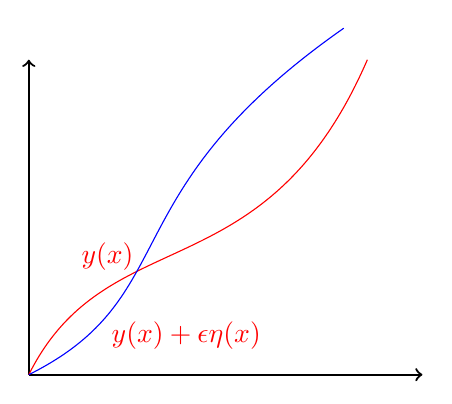
\begin{tikzpicture}
		\draw[->,thick] (0,0) -- (5,0);
		\draw[->,thick] (0,0) -- (0,4);
		
		\draw[red] (0,0) .. controls (1,2) and (3,1)  ..(4.3,4) node at (1,1.5){$y(x)$};
		\draw[blue] (0,0) .. controls (2,1) and (1,2.3).. (4,4.4) node at (2,0.5){$y(x)+\epsilon\eta(x)$};
	\end{tikzpicture}
\end{center}
我们把泛函$F[y]$关于$y(x)$的导数记作$\frac{\delta F}{\delta y(x)}$,通过下面的关系定义
\begin{equation}
\label{zhuanhua}
	F[y(x)+\epsilon\eta(x)]=F[y(x)]+\epsilon\int \frac{\delta F}{\delta y(x)}\eta(x) dx + O(\epsilon^2)
\end{equation}
这可以被看成公式$\ref{tuiguang}$的一个自然推广,其中$F[y]$现在依赖于变量的一个连续集合,即在所有$x$处的$y$值。令泛函的值在函数$y(x)$发生微小改变时几乎不变,可得
\begin{equation}
	\int \frac{\delta F}{\delta y(x)}\eta(x) dx=0
\end{equation}
由于这必须对任意的$\eta(x)$都成立,因此我们必须令泛函的导数等于零。为了证明这一点,让我们假设选择一个扰动$\eta(x)$,这个扰动只在点$\hat{x}$的邻域内等于零,在其他各处均不等于零。这种情况下,泛函的导数必须在$x=\hat{x}$处等于零。但是,由于这个结论必须对于任意的$\hat{x}$f都成立,因此泛函的导数必须对所有的$x$值都等于零。

考虑一个泛函,这个泛函由函数$G(y,y^{'},x)$的积分定义。函数$G(y,y^{'},x)$既依赖于$y(x)$又依赖于它的导数$y^{'}(x)$,还直接依赖于$x$。因此,这个泛函的形式为
\begin{equation}
	F[y]=\int G(y(x),y^{'}(x),x)dx
\end{equation}
其中,我们假设$y(x)$的值在积分边界(可能是无穷)处是定值。如果我们考虑函数$y(x)$的改变,那么我们有
\begin{equation}
	F[y(x)+\epsilon\eta(x)]=F[y(x)]+\epsilon\int \left\{\frac{\partial G}{\partial y}\eta(x)+\frac{\partial G}{\partial y^{'}}\eta^{'}(x) \right\}dx +O(\epsilon^2)
\end{equation}
我们现在必须把它转化为公式$\ref{zhuanhua}$的形式。为了完成这一点,我们将第二项进行分部积分,然后使用$\eta(x)$必须在积分边界处等于零的事实(因为$y(x)$在边界处为定值)。因此
\begin{equation}
		F[y(x)+\epsilon\eta(x)]=F[y(x)]+\epsilon\int \left\{\frac{\partial G}{\partial y}-\frac{d}{dx }\left(\frac{\partial G}{\partial y^{'}} \right) \right\}\eta(x)dx +O(\epsilon^2)
\end{equation}
我们可以直接读出泛函的导数。令泛函的导数等于零,我们有
\begin{equation}
	\frac{\partial G}{\partial y} - \frac{d}{dx}\left(\frac{\partial G}{\partial y^{'}} \right)=0
\end{equation}
这被称为欧拉-拉格朗日方程(Euler-Lagrange equation)。例如,如果
\begin{equation}
	G=y(x)^2+(y^{'}(x))^2
\end{equation}
那么,欧拉-拉格朗日方程的形式为
\begin{equation}
	y(x)-\frac{d^2y}{dx^2}=0
\end{equation}
使用$y(x)$的边界条件,我们可以解出这个关于$y(x)$的二阶微分方程。

通常情况下,我们考虑定义在积分上的泛函时,被积函数的形式为$G(y,x)$,不依赖于$y(x)$的导数。这种情况下,驻点只需要令$\frac{\partial G}{\partial y(x)}=0$对于所有的$x$都成立即可。

如果我们关于概率分布对泛函进行优化,那么我们需要保持概率的归一化限制。使用拉格朗日乘数法来进行优化是最方便的。使用拉格朗日乘数法之后,我们就可以进行无限制条件的最优化。

上述结果在多维变量$\boldsymbol{x}$上的扩展是很直接的。
\chapter{矩阵的性质}
\section{矩阵的基本性质}
矩阵$A$的第$i$行和第$j$列的元素为$A_{ij}$。我们用$I_N$表示$N\times N$的单位矩阵。在没有歧义的情形下,我们简单地记作$I$。转置矩阵$A^T$的元素为$(A^T)_{ij}=A_{ji}$。根据转置的定义,我们有
\begin{equation}
	(AB)^T=B^TA^T
\end{equation}
$A$的逆矩阵,记作$A^{-1}$,满足
\begin{equation}
	AA^{-1}=A^{-1}A=I
\end{equation}
由于$ABB^{-1}A^{-1}=I$,我们有
\begin{equation}
\label{c3}
	(AB)^{-1}=B^{-1}A^{-1}
\end{equation}
我们还有
\begin{equation}
	(A^T)^{-1}=(A^{-1})^T
\end{equation}
关于矩阵的逆矩阵,下面这个恒等式很有用
\begin{equation}
\label{guji}
	(P^{-1}+B^TR^{-1}B)^{-1}B^TR^{-1}=PB^T(BPB^T+R)^{-1}
\end{equation}
两侧同时右乘$(BPB^T+R)$,很容易证明上式的正确性。假设$P$的维度为$N\times N$,而$R$的维度为$M\times M$,从而$B$的维度为$M\times N$。这样,如果$M\ll N$,那么估计公式$\ref{guji}$的右侧所花费的低价就远远小于估计左侧的代价。经常出现的一种情况是
\begin{equation}
	(I+AB)^{-1}A=A(I+BA)^{-1}
\end{equation}
另一个与矩阵的逆矩阵相背的有用的恒等式为
\begin{equation}
	(A+BD^{-1}C)^{-1}=A^{-1}-A^{-1}B(D+CA^{-1}B)^{-1}CA^{-1}
\end{equation}
这被称为Woodbury恒等式。将两侧同时乘以$(A+BD^{-1}C)$即可证明。例如,假设$A$是一个很大的对角矩阵(因此很容易求逆矩阵),$B$的行数很多列数很少($C$恰好相反),此时计算右侧的代价就远远小于计算左侧的代价。

一组向量$\{a_1,\dots,a_N\}$被称为线性相关(linearly independent)如果关系$\sum_n a_n \boldsymbol{a}_n=0$只在所有$a_n=0$时成立。这表明,没有任何一个向量能够表示为其余向量的线性组合。矩阵的秩是线性无关的行的最大数量(或者等价地,线性无关的列的最大数量)。
\section{迹和行列式}
迹和行列式适用于方阵。矩阵$A$的迹$\mathrm{Tr}(A)$被定义为主对角线上元素的和。我们可以看到
\begin{equation}
	\mathrm{Tr}(AB)=\mathrm{Tr}(BA)
\end{equation}
通过多次把这个公式应用到三个矩阵的乘积上,我们看到
\begin{equation}
	\mathrm{Tr}(ABC)=\mathrm{Tr}(CAB)=\mathrm{Tr}(BCA)
\end{equation}
这被称为迹操作符的循环(cyclic)性质。很明显这个性质可以扩展到任意数量矩阵的乘积。一个$N\times N$矩阵的行列式$|A|$定义为
\begin{equation}
	|A|=\sum (\pm 1)A_{1i_1}A_{2i_2}\dots A_{Ni_N}
\end{equation}
这个式子对所有满足下面性质的乘积进行求和:乘积包含每行的恰好一个元素和每列的恰好一个元素。系数$+1$或者$-1$取决于排列$i_1\dots i_N$是大奇排列还是偶排列。注意$|I|=1$,因此对于一个$2\times 2$矩阵,行列式的形式为
\begin{equation}
	|A|=\begin{vmatrix}
		a_{11}&a_{12}\\
		a_{21}&a_{22}
	\end{vmatrix}
	=a_{11}a_{22}-a_{12}a_{21}
\end{equation}
两个矩阵乘积的行列式为
\begin{equation}
\label{c12}
	|AB|=|A||B|
\end{equation}
此外,矩阵的逆矩阵的行列式为
\begin{equation}
	|A^{-1}|=\frac{1}{|A|}
\end{equation}
如果$A$和$B$是$N\times M$的矩阵,那么 
\begin{equation}
	|I_N+AB^T|=|I_M+A^TB|
\end{equation}
一种特殊情况是
\begin{equation}
	|I_N+ab^T|=1+a^Tb
\end{equation}
其中$a$和$b$是N维列向量。
\section{矩阵的导数}
有时,我们需要考虑向量和矩阵关于标量的导数。向量$\boldsymbol{a}$关于标量$x$的导数本身是一个向量,它的分量为
\begin{equation}
	\left(\frac{\partial \boldsymbol{a}}{\partial x} \right)_i=\frac{\partial a_i}{\partial x}
\end{equation}
矩阵的导数的定义与些类似。关于向量和矩阵的导数也可以被定义。例如
\begin{equation}
	\left(\frac{\partial x}{\partial \boldsymbol{a}} \right)_i=\frac{\partial x}{\partial a_i}
\end{equation}
类似地
\begin{equation}
	\left(\frac{\partial a}{\partial b} \right)_{ij}=\frac{\partial a_i}{\partial b_j}
\end{equation}
写出矩阵的各个元素,下面的性质很容易证明
\begin{equation}
	\frac{\partial }{\partial \boldsymbol{x}}(\boldsymbol{x}^T\boldsymbol{a})=\frac{\partial }{\partial \boldsymbol{x}}(\boldsymbol{a}^T\boldsymbol{x})=\boldsymbol{a}
\end{equation}
类似地
\begin{equation}
\label{weifen}
	\frac{\partial }{\partial \boldsymbol{x}}(AB)=\frac{\partial A}{\partial \boldsymbol{x}}B+A\frac{\partial B}{\partial \boldsymbol{x}}
\end{equation}
矩阵的逆矩阵的导数可以表示为
\begin{equation}
	\frac{\partial }{\partial x}(A^{-1})=-A^{-1}\frac{\partial A}{\partial x}A^{-1}
\end{equation}
使用公式$\ref{weifen}$对方程$A^{-1}A=I$求微分,然后右乘$A^{-1}$即可证明。并且 
\begin{equation}
	\frac{\partial }{\partial x}\ln |A|=\mathrm{Tr}\left(A^{-1}\frac{\partial A}{\partial x} \right)
\end{equation}
如果我们把$x$选成$A$中的元素,那么我们有
\begin{equation}
	\frac{\partial }{\partial A_{ij}}\mathrm{Tr}(AB)=B_{ji}
\end{equation}
写出矩阵的下标即可证明这个等式。我们可以把这个结论写成更加简洁的形式
\begin{equation}
	\frac{\partial }{\partial A}\mathrm{Tr}(AB)=B^T
\end{equation}
使用这种记号,我们有下列性质 
\begin{flalign}
	\frac{\partial }{\partial A}\mathrm{Tr}(A^TB)&=B\\
	\frac{\partial }{\partial A}\mathrm{Tr}(A)&=I\\
	\frac{\partial }{\partial A}\mathrm{Tr}(ABA^T)&=A(B+B^T)
\end{flalign}
这些也可以通过写出矩阵下标的方式证明出。我们也有
\begin{equation}
	\frac{\partial }{\partial A}\ln |A|=(A^{-1})^T
\end{equation}

\section{特征向量方程}
对于一个$M\times M$的方阵$A$,特征向量方程的定义为
\begin{equation}
\label{luqu}
	\boldsymbol{A}\boldsymbol{\mu}_i=\lambda_i\boldsymbol{\mu}_i
\end{equation}
其中$i=1,\dots,M$,$\boldsymbol{\mu}_i$被称为特征向量(eigenvector),$\lambda_i$被称为对应的特征值(eigenvalue)。这可以看成M个齐次线性方程组,角存在的条件为
\begin{equation}
	|A-\lambda_i I|=0
\end{equation}
这被称为特征方程(characteristic equation)。由于这是$\lambda_i$的M阶多项式,因此它一定有M个解(虽然这些解未必不同)。$A$的秩等于非零特征值的个数。

我们特别感兴趣的是对称矩阵。协方差矩阵、核矩阵、Hessian矩阵都是对称矩阵。对称矩阵的性质为$A_{ij}=A_{ji}$或者等价地,$A=A^T$。对称矩阵的逆矩阵也是对称的。将$A^TA=I$取转置,然后使用$AA^{-1}=I$以及$I$的对称性即可证明这一点。

通常情况下,矩阵的特征值是复数。但是对于对称矩阵,特征值$\lambda_i$为实数。这点可以用下面的方式证明。首先将公式$\ref{luqu}$左乘$(\boldsymbol{\mu}_i^*)^T$,其中$*$表示复共轭,我们可以得到 
\begin{equation}
	(\boldsymbol{\mu}_i^*)^TA\boldsymbol{\mu}_i=\lambda_i(\boldsymbol{\mu}_i^*)^T\boldsymbol{\mu}_i
\end{equation}
之后,我们对公式$\ref{luqu}$取复共轭,然后左乘$\boldsymbol{\mu}_i^T$,可得
\begin{equation}
	\boldsymbol{\mu}_i^TA\boldsymbol{\mu}_i^*=\lambda_i^*\boldsymbol{\mu}_i^T\boldsymbol{\mu}_i^*
\end{equation}
推导过程中,我们使用了$A^*=A$,因为我们只考虑实对称矩阵$A$。将第二个方程取转置,使用$A^T=A$,我们看到两个方程在左侧相同,从而$\lambda_i^*=\lambda_i$,因此$\lambda_i$一定是实数。

实对称矩阵的特征向量$\boldsymbol{\mu}_i$可以被选成单位正交的(即正交的并且长度为单位长度),使得
\begin{equation}
	\boldsymbol{\mu}_i^T\boldsymbol{\mu}_j=I_{ij}
\end{equation}
其中$I_{ij}$是单位矩阵$I$的元素。为了证明这一点,我们首先将公式$\ref{luqu}$左乘$\boldsymbol{\mu}_j^T$,得到 
\begin{equation}
	\boldsymbol{\mu}_j^T\boldsymbol{A}\boldsymbol{\mu}_i=\lambda_i\boldsymbol{\mu}_j^T\boldsymbol{\mu}_i
\end{equation}
因此,通过交换下标,我们有
\begin{equation}
	\boldsymbol{\mu}_i^T\boldsymbol{A}\boldsymbol{\mu}_j=\lambda_j\boldsymbol{\mu}_i^T\boldsymbol{\mu}_j
\end{equation}
我们现在对第二个方程取转置,使用对称性质$\boldsymbol{A}^T=\boldsymbol{A}$,然后将两个方程相减,可得
\begin{equation}
	(\lambda_i-\lambda_j)\boldsymbol{\mu}_i^T\boldsymbol{\mu}_j=0
\end{equation}
因此,对于$\lambda_i\ne \lambda_j$,我们有$\boldsymbol{\mu}_i^T\boldsymbol{\mu}_j=0$,因此$\boldsymbol{\mu}_i$和$\boldsymbol{\mu}_j$是正交的。如果两个特征值是相等的,那么任意线性组合$\alpha \boldsymbol{\mu}_i+\beta \boldsymbol{\mu}_j$也是一个有着相同特征值的特征向量,因此我们可以任意选择一个线性组合,然后选择第二个特征向量正交于第一个(可以证明这种退化的特征向量永远不会线性相关)。因此特征向量可以选择为正交的,然后归一化为单位长度。由于有M个特征值,对应的M个特征向量组成了一个完备集,因此任意一个M维的向量都可以表示为特征向量的线性组合。

我们可以令特征向量$\boldsymbol{\mu}_i$是$M\times M$的矩阵$\boldsymbol{U}$,根据单位正交性,我们有
\begin{equation}
\label{zhengming}
	\boldsymbol{U}^T\boldsymbol{U}=\boldsymbol{I}
\end{equation}
这样的矩阵被称为正交的(orthogonal)。有趣的是,矩阵的行也是正交的,即$\boldsymbol{U}\boldsymbol{U}^T=\boldsymbol{I}$。为了证明这一点,我们注意到,公式$\ref{zhengming}$表明$\boldsymbol{U}^T\boldsymbol{U}\boldsymbol{U}^{-1}=\boldsymbol{U}^{-1}=\boldsymbol{U}^T$,因此$\boldsymbol{U}\boldsymbol{U}^{-1}=\boldsymbol{U}\boldsymbol{U}^T=\boldsymbol{I}$。使用公式$\ref{c12}$,也可以看出$|U|=1$。

特征向量方程$\ref{luqu}$可以使用$\boldsymbol{U}$表示成下面的形式
\begin{equation}
\label{c38}
	\boldsymbol{AU}=\boldsymbol{U\Lambda}
\end{equation}
其中$\boldsymbol{\Lambda}$是一个$M\times M$的对角矩阵,对角线上的元素为特征值$\lambda_i$。

如果我们考虑一个列向量$\boldsymbol{x}$,它经过正交矩阵$\boldsymbol{U}$进行变换,得到新向量 
\begin{equation}
	\tilde{\boldsymbol{x}}=\boldsymbol{Ux}
\end{equation}
变换前后向量的长度不变,因为 
\begin{equation}
	\tilde{\boldsymbol{x}}^T\tilde{\boldsymbol{x}}=\boldsymbol{x}^T\boldsymbol{U}^T\boldsymbol{U}\boldsymbol{x}=\boldsymbol{x}^T\boldsymbol{x}
\end{equation}
类似地,任意两个向量的角度在变换前后也不变,因为
\begin{equation}
	\tilde{\boldsymbol{x}}^T\tilde{\boldsymbol{y}}=\boldsymbol{x}^T\boldsymbol{U}^T\boldsymbol{U}\boldsymbol{y}=\boldsymbol{x}^T\boldsymbol{y}
\end{equation}
因此,乘以$\boldsymbol{U}$可以表示为坐标第的刚性旋转.

根据公式$\ref{c38}$可得
\begin{equation}
	\boldsymbol{U}^T\boldsymbol{AU}=\boldsymbol{\Lambda}
\end{equation}
因为$\boldsymbol{\Lambda}$是对角矩阵,我们说矩阵$\boldsymbol{A}$被矩阵$\boldsymbol{U}$对角化(diagonalised)。如果我们左乘$\boldsymbol{U}$然后右乘$\boldsymbol{U}^T$,我们有
\begin{equation}
\label{c43}
	\boldsymbol{A}=\boldsymbol{U\Lambda U}^T
\end{equation}
取这个方程的逆,然后使用公式$\ref{c3}$以及$\boldsymbol{U}^{-1}=\boldsymbol{U}^T$,我们有
\begin{equation}
	\boldsymbol{A}^{-1}=\boldsymbol{U}\boldsymbol{\Lambda}^{-1}\boldsymbol{U}^T
\end{equation}
最后两个方程也可以写成 
\begin{flalign}
	\boldsymbol{A}&=\sum_{i=1}^{M}\lambda_i\boldsymbol{\mu}_i\boldsymbol{\mu}_i^T\\
	\boldsymbol{A}^{-1}&=\sum_{i=1}^{M}\frac{1}{\lambda_i}\boldsymbol{\mu}_i\boldsymbol{\mu}_i^T
\end{flalign}
如果我们取公式$\ref{c43}$的行列式,然后使用公式$\ref{c12}$,我们有
\begin{equation}
	|\boldsymbol{A}|=\prod_{i=1}^{M}\lambda_i
\end{equation}
类似地,取公式$\ref{c43}$的迹,使用迹运算的循环性以及$\boldsymbol{U}^T\boldsymbol{U}^T=\boldsymbol{I}$,我们有
\begin{equation}
	\mathrm{Tr}(\boldsymbol{A})=\sum_{i=1}^{M}\lambda_i
\end{equation}

一个矩阵$\boldsymbol{A}$被称为正定的(positive definite),记作$\boldsymbol{A}\succ 0$,如果对于向量$\boldsymbol{w}$的所有非零值都有$\boldsymbol{w}^T\boldsymbol{Aw}>0$。等价地,一个正定矩阵的所有特征值都有$\lambda_i>0$。令$\boldsymbol{w}$为每一个特征向量,然后注意到任意的向量都可以展开为特征向量的组合,我们即可以证明这一点。注意,正定不同于所有元素都为正。例如,矩阵
\begin{equation}
	\begin{pmatrix}
		1&2\\
		3&4
	\end{pmatrix}
\end{equation}
的特征值$\lambda_1 \simeq 5.37$且$\lambda_2\simeq -0.37$。一个矩阵被称为半正定的(positive semidefinite),如果对于$\boldsymbol{w}$的所有值都有$\boldsymbol{w}^T\boldsymbol{Aw}\geqslant 0$,记作$\boldsymbol{A}\succeq 0$。它等价于$\lambda_i \geqslant 0$。
\chapter{信息论}
信息量可以被看成在学习$x$的值的时候的“惊讶程度”。我们对于信息内容的度量将依赖于概率分布$p(x)$,因此我们想要寻找一个函数$h(x)$,它是概率$p(x)$的单调递增函数,表达了信息的内容。$h(\cdot)$的形式可以这样寻找:如果我们有两个不相关的事件$x$和$y$,那么我们观察到两个事件同时发生时获得的信息应该等于观察到事件各自发生时获得的信息之和,即$h(x,y)=h(x)+h(y)$。两个不相关事件是统计独立的,因此$p(x,y)=p(x)p(y)$。根据这两个关系,很容易看出$h(x)$一定与$p(x)$对数有关。因此,我们有
\begin{equation}
\label{192}
	h(x)=-\log_2p(x)
\end{equation}
其中,负号确保了信息一定是正数或者是零。注意,低概率事件$x$对应于高的信息量。对数的底的选择是任意的。

现在假设一个发送者想传输一个随机变量的值给接收者。这个过程中,他们传输的平均信息量可以通过求公式$\ref{192}$关于概率分布$p(x)$的期望得到。这个期望值为
\begin{equation}
	H[x]=-\sum_xp(x)\log_2p(x)
\end{equation}
这个重要的量被叫做随机变量$x$的熵(entropy)。无噪声编码定理(noiseless coding theorem)表明,熵是传输一个随机变量状态值所需的比特位的下界。

我们已经通过具体化随机变量的状态所需的平均信息量介绍了熵的概念。事实上,熵的概念最早起源于物理学,是在热力学平衡的背景中介绍的。后来,熵成为描述统计力学中的无序程度的度量。我们可以这样理解熵的这种含义:考虑一个集合,包含N个完全相同的物体,这些物体要被分到若干个箱子中,使得第$i$个箱子中有$n_i$。考虑把物体分配到箱子中的不同方案的数量。有N种方式选择第一个物体,有$(N-1)$种方式选择第二个物体,以此类推。因此总共有$N!$种方式把N个物体分配到箱子中。然而,我们不想区分每个箱子内部物体的重新排列。有第$i$个箱子中,有$n_i!$种方式对物体重新排序,因此把N个物体分配到箱子中的总方案数量为
\begin{equation}
	W=\frac{N!}{\prod_{i}n_i!}
\end{equation}
这被称为乘数(multiplicity)。熵被定义为通过适当的参数放缩后的对数乘数,即
\begin{equation}
	H=\frac{1}{N}\ln W=\frac{1}{N}\ln N! = \frac{1}{N}\sum_i \ln n_i!
\end{equation}
我们现在考虑极限$N\to \infty$,并且保持比值$\frac{n_i}{N}$固定,使用Stirling的估计
\begin{equation}
	\ln N!\simeq N\ln N - N
\end{equation}
可以得到
\begin{equation}
	H=-\lim_{N\to \infty} \sum_i \left(\frac{n_i}{N}\right)\ln\left(\frac{n_i}{N}\right)=-\sum_ip_i\ln p_i
\end{equation}
推导时我们使用了$\sum_i n_i = N$。使用物理学的术语,箱子中物体的具体分配方案被称为微观状态(microstate),整体的占领数的分布,表示为比值$\frac{n_i}{N}$,被称为宏观状态(macrostate)。乘数W也被称为宏观状态的权重(weight)。

在概率归一化的限制下,使用拉格朗日乘数法可以找到熵的最大值。因此,我们要最大化
\begin{equation}
	\tilde{H}=-\sum_ip(x_i)\ln p(x_i)+\lambda \left(\sum_ip(x_i)-1 \right)
\end{equation}
可以证明,当所有的$p(x_i)$都相等,且值为$p(x_i)=\frac{1}{M}$时,熵取得最大值。其中,$M$是状态$x_i$的总数。此时对应的熵值为$H=\ln M$。这个结果也可以通过Jensen不等式推导出来。

我们可以把熵的定义扩展到连续变量$x$的概率分布$p(x)$。方法如下,首先把$x$切分成宽度为$\triangle$的箱子。然后假设$p(x)$是连续的。
\begin{equation}
	H[x]=\lim_{\triangle\to 0}-\sum_ip(x_i)\ln p(x_i)\left\{ \right\}=-\int p(x)\ln p(x)dx
\end{equation}
其中,右侧的量被称为微分熵(differential entropy)。我们看到,熵的离散形式与连续形式的差是$\ln \triangle$,这在极限$\triangle\to 0$的情形下发散。这反映同一个事实:具体化一个连续变量需要大量的比特位。

在离散分布的情况下,我们看到最大熵对应于变量的所有可能状态的均匀分布。现在让我们考虑连续变量的最大熵。为了让最大值有一个合理一定义,有必要限制$p(x)$的一阶矩和二阶矩,同时要保留归一化的限制。因此
我们要优化下面的关于$p(x)$的函数
\begin{equation}
	\begin{aligned}
		-\int_{-\infty}^{+\infty}p(x)\ln p(x)dx+\lambda_1\left(-\int_{-\infty}^{+\infty}p(x)-1 \right)
		+\lambda_2\left(-\int_{-\infty}^{+\infty}xp(x)dx-\mu \right)\\+\lambda_3\left(-\int_{-\infty}^{+\infty}(x-\mu)^2p(x)dx -\sigma^2\right)
	\end{aligned}
\end{equation}
使用变分法中,令这个函数的导数等于零,我们有
\begin{equation}
	p(x)=\exp\{-1+\lambda_1+\lambda_2x+\lambda_3(x-\mu)^2\}
\end{equation}
将这个结果代入三个限制方程中,即可求出拉格朗日乘数,最终的结果为
\begin{equation}
	p(x)=\frac{1}{(2\pi\sigma^2)^{\frac{1}{2}}}\exp\left\{-\frac{(x-\mu)^2}{2\sigma^2} \right\}
\end{equation}
因此最大化微分熵的分布是高斯分布。求解高斯分布的微分熵
\begin{equation}
	\begin{aligned}
		H[x]&=-\int \frac{1}{(2\pi\sigma^2)^{\frac{1}{2}}}\exp\left\{-\frac{(x-\mu)^2}{2\sigma^2} \right\}\ln \frac{1}{(2\pi\sigma^2)^{\frac{1}{2}}}\exp\left\{-\frac{(x-\mu)^2}{2\sigma^2} \right\}dx\\
		&=-\frac{1}{(2\pi\sigma^2)^{\frac{1}{2}}}\int \exp\left\{-\frac{(x-\mu)^2}{2\sigma^2} \right\}\left(-\ln(\sqrt{2\pi}\sigma)-\frac{(x-\mu)^2}{2\sigma^2} \right)dx\\
		&=\frac{\ln(\sqrt{2\pi\sigma}}{(2\pi\sigma^2)^{\frac{1}{2}}}\int \exp\left\{-\frac{(x-\mu)^2}{2\sigma^2} \right\}dx+\frac{1}{(2\pi\sigma^2)^{\frac{1}{2}}}\int \exp\left\{-\frac{(x-\mu)^2}{2\sigma^2} \right\}\frac{(x-\mu)^2}{2\sigma^2}dx\\
		&=\frac{\ln(\sqrt{2\pi\sigma}}{(2\pi\sigma^2)^{\frac{1}{2}}}\sqrt{2}\sigma\int \exp\left\{-\left(\frac{x-\mu}{\sqrt{2\sigma}}\right)^2 \right\}d\left(\frac{x-\mu}{\sqrt{2\sigma}}\right)\\
		&\ \ + \frac{1}{(2\pi\sigma^2)^{\frac{1}{2}}}\sqrt{2}\sigma\int \exp\left\{-\left(\frac{x-\mu}{\sqrt{2\sigma}}\right)^2 \right\}\frac{(x-\mu)^2}{2\sigma^2}d\left(\frac{x-\mu}{\sqrt{2\sigma}}\right)\\
		&=\frac{\ln (\sqrt{2\pi}\sigma)}{\sqrt{\pi}}\int_{-\infty}^{+\infty}\exp (-y^2)dy+\frac{1}{\sqrt{\pi}}\int_{-\infty}^{+\infty}\exp (-y^2)y^2dy\\
		&=\ln(\sqrt{2\pi}\sigma)+\frac{1}{\sqrt{\pi}}\cdot -\frac{1}{2}\left(0-\int_{-\infty}^{+\infty}\exp(-y^2)dy \right)\\
		&=\ln(\sqrt{2\pi}\sigma)+\frac{1}{2}\\
		&=\frac{1}{2}\left(\ln(2\pi \sigma^2)+1\right)
	\end{aligned}
\end{equation}

假设我们有一个联合概率分布$p(x,y)$。当我们从这个概率分布中抽取了一对$x$和$y$。如果$x$的值已知,那么需要确定对应的$y$值所需的附加的信息就是$-\ln p(y|x)$。因此,用来确定$y$值的平均附加信息可以写成
\begin{equation}
	H[y|x]=-\iint p(y,x)\ln p(y|x)dydx
\end{equation}
这被称为给定$x$的情况下,$y$的条件熵。使用乘积规则,很容易看出,条件熵满足下面的关系 
\begin{equation}
	H[x,y]=H[y|x]+H[x]
\end{equation}
其中,$H[x,y]$是$p(x,y)$的微分熵,$H[x]$是边缘分布$p(x)$的微分熵。因此,描述$x$和$y$所需的信息是描述$x$自己抽需的信息,加上给定$x$的情况下具体化$y$所需的额外信息。

\subsection*{相对熵和互信息}
目前为止,我们已经介绍了信息论的许多概念,包括熵的关键思想。现在开始把这些思想关联到模式识别的问题中。考虑某个未知的分布$p(x)$,假定我们已经使用一个近似的分布$q(x)$对它进行了建模。如果我们使用$q(x)$来建立一个编码体系,用来把$x$的值传给接收者,那么,由于我们使用了$q(x)$而不是真实分布$p(x)$,因此在具体化$x$的值时,我们需要一些附加的信息。我们需要的平均的附加信息量为
\begin{equation}
	\begin{aligned}
		\mathrm{KL}(p\| q)&=-\int p(x)\ln q(x)dx-\left(-\int p(x)\ln p(x)dx\right)\\
		&=-\int p(x)\ln \left\{\frac{q(x)}{p(x)} \right\}dx
	\end{aligned}
\end{equation}
这被称为分布$p(x)$和分布$q(x)$之间的相对熵(relative entropy)或者Kullback-Leibler散度(Kullback-Leibler divergence),或者KL散度。注意这不是一个对称量,即$\mathrm{KL}(p\| q)\neq  \mathrm{KL}(q\| p)$

\begin{equation}
	\mathrm{KL}(p\| q)=-\int p(x)\ln \left\{\frac{q(x)}{p(x)} \right\}dx \geqslant -\ln \int q(x)dx=0
\end{equation}
推导过程中,我们使用了$-\ln x$是凸函数的事实,以及归一化条件$\int q(x)dx=1$和Jensen不等式。

我们看到,在数据压缩和密度估计(即对未知概率分布建模)之间有一种隐含的关系,因为当我们知道真实的概率分布之后,我们可以给出最有效的压缩。如果我们使用了不同于真实分布的概率分布,那么我们一定会损失编码效率,并且在传输时增加的平均额外信息量至少等于两个分布之间的Kullback-Leibler散度。

假设数据通过未知分布$p(x)$生成,我们想要对$p(x)$建模。我们可以试着使用一些参数分布$q(x|\theta)$来近似这个分布。$q(x|\theta)$由可调节的参数$\theta$控制。一种确定$\theta$的方式是最小化$p(x)$和$q(x|\theta)$之间关于$\theta$的Kullback-Leibler散度。我们不能直接这么做,因为我们不知道$p(x)$。但是,假设我们已经观察到了服从分布$p(x)$的有限数量的训练点$x_n$,其中$n=1,\dots,N$。那么,关于$p(x)$的期望就可以通过这些点的有限加和,使用公式来近似
\begin{equation}
	\mathrm{KL}(p\| q)\simeq \frac{1}{N}\sum_{n=1}^{N}\{-\ln q(x_n|\theta)+\ln p(x_n) \}
\end{equation}
公式右侧的第二项与$\theta$无关,第一项是使用训练集估计的分布$q(x|\theta)$下的$\theta$的负对数似然函数。因此我们看到,最小化Kullback-Leibler散度等价于最大化似然函数。

现在考虑由$p(x,y)$给出的两个变量$x$和$y$组成的数据集。如果变量的集合是独立的,那么他们的联合分布可以分解为边缘分布的乘积$p(x,y)=p(x)p(y)$。如果变量不是独立的,那么我们可以通过考察联合概率分布与边缘概率分布乘积之间的Kullback-Leibler散度来判断它们是否“接近”于相互独立。此时,Kullback-Leibler散度为
\begin{equation}
	\begin{aligned}
		I[x,y]&\equiv \mathrm{KL}(p(x,)\| p(x)p(y))\\
		&=-\iint p(x,y)\ln \left(\frac{p(x)p(y)}{p(x,y)}\right)dxdy
	\end{aligned}
\end{equation}
这被称为变量$x$和变量$y$之间的互信息(mutual information)。根据Kullback-Leibler散度的性质,我们看到$I[x,y]\geqslant 0$,当且仅当$x$和$y$相互独立时等号成立。互信息和条件熵之间的关系为
\begin{equation}
	I[x,y]=H[x]-H[x|y]=H[y]-H[y|x]
\end{equation}
因此我们可以把互信息看成由于知道$y$值而造成的$x$的不确定性的减小(反这亦然)。从贝叶斯的观点来年,我们可以把$p(x)$看成$x$的先验概率分布,把$p(x|y)$看成我们观察到新数据$y$之后的后验概率分布。因此互信息表示一个新的观测$y$造成的$x$的不确定性的减小。
\chapter{回归的线性模型}
目前为止,关注点是无监督学习,包括诸如概率密度估计和数据聚类等话题。我们现在开始讨论有监督学习,首先讨论的是回归问题。回归问题的目标是在给定$D$维输入(input)变量$\boldsymbol{x}$的情况下,预测一个或者多个连续目标(target)变量$t$的值。线性回归模型有着可调节的参数,具有线性函数的性质,将会成为本章的关注点。线性回归模型的最简单的形式也是输入变量的线性函数。但是,通过将一组输入变量的非线性函数进行线性组合,我们也可以获得一类更加有用的函数,被称为基函数(basis function)。这样的模型是参数的线性模型,这使得其具有一些简单的分析性质,同时关于输入变量是非线性的。

最简单的方法是,直接建立一个适当的函数$y(\boldsymbol{x})$,对于新的输入$\boldsymbol{x}$,这个函数能够直接给出对应的$t$预测。更一般地,从一个概率的观点来看,我们的目标是对预测分布$p(t|\boldsymbol{x})$建模,因为经表达了对于每个$\boldsymbol{x}$的值,我们对于$t$的值的不确定性。从这个条件概率分布中,对于任意的$\boldsymbol{x}$的新值,我们可以对$t$进行预测,这种方法等同于最小化一个恰当的损失函数的期望值。对于实值变量来说,损失函数的一个通常的选择是平方误差损失,这种情况下最优解由$t$的条件期望给出。
\section{线性基函数模型}
回归问题的最简单模型是输入变量的线性组合
$$
y(\boldsymbol{x,w})=w_0+w_1x_1 + \dots w_Dx_D
$$
其中$x=(x_1,\dots,x_D)^T$。这通常被简单地称为\textbf{线性回归(linear regression)}。这个模型的关键性质是它是参数$w_0,\dots,w_D$的一个线性函数。但是,它也是输入变量$x_i$的一个线性函数,这给模型带来了极大的局限性。因此,我们扩展模型的类别:将输入变量的固定的非线性函数进行线性组合,形式为
$$
y(\boldsymbol{x,w})=w_0+\sum_{y=1}^{M-1}w_j\phi_j(\boldsymbol{x})=\sum_{j=0}^{M-1}w_j\phi_j(\boldsymbol{x})=\boldsymbol{w}^T\phi(\boldsymbol{x})
$$
其中$\phi_j(\boldsymbol{x})$被称为基函数(basis function)。
\begin{enumerate}
	\item 高斯基函数 
	$$
	\phi_j(x)=exp\left\{-\frac{(x-\mu_j)^2}{2s^2}\right\}
	$$
	\item sigmoid基函数 
	$$
	\phi_j(x)=\frac{1}{1+exp\left(\frac{x-\mu_j}{s}\right)}
	$$
	\item 傅里叶基函数
\end{enumerate}
\section{偏置-方差分解}
目前为止,我们对于回归的线性模型的讨论中,我们假定了基函数的形式和数量都是固定的。如果使用有限规模的数据集来训练复杂的模型,那么使用最大似然法,或者等价地使用最小平方法,会导致严重的过拟合问题。正如前面所说,过拟合现象确实是最大似然方法的一个不好的性质。但是当我们在使用贝叶斯方法对参数进行求和或者积分时,过拟合现象不会出现。从贝叶斯观点讨论模型的复杂度之前,从频率学家的观点考虑一下模型的复杂度的问题——偏置-方差折中(bias-variance trade-off)。

最优的预测(变分法可求出)由条件期望(记作$h(x)$)给出,即
\begin{equation}
	h(x)=\mathbb{E}[t|x]=\int tp(t|x)dt
\end{equation}
平方损失函数的期望可以写成
\begin{equation}
\label{llk}
\begin{aligned}
	\mathbb{E}[L]&=\iint \{y(x)-h(x)\}^2p(x,t)dxdt\\
	&=\int \{y(x)-h(x) \}^2p(x)dx + \iint \{h(x)-t\}^2p(x,t)dxdt\\
\end{aligned}
\end{equation}
考虑第一项的被积函数,对于一个特定的数据集$D$,它的形式为
\begin{equation}
	\{y(x;D)-h(x)\}^2
\end{equation}
由于这个量与特定的数据集$D$相关,因此我们对所有的数据集取平均。如果我们在括号内加上然后减去$\mathbb{E}_D[y(x;D)]$,然后展开,我们有
\begin{equation}
	\begin{aligned}
		\{y(x;D)&-\mathbb{E}_D[y(x;D)]+\mathbb{E}_D[y(x;D)] -h(x) \}^2\\
		&=\{y(x;D)-\mathbb{E}_D[y(x;D)]\}^2\\
		&+\{\mathbb{E}_D[y(x;D)]-h(x) \}^2\\
		&+ 2\{y(x;D)-\mathbb{E}_D[y(x;D)]\}\{\mathbb{E}_D[y(x;D)]-h(x) \}
	\end{aligned}
\end{equation}
现在关于$D$求期望,然后注意到\textbf{最后一项等于零},可得
\begin{equation}
\label{kk}
\begin{aligned}
	\mathbb{E}_D&[\{y(x;D)-h(x) \}^2]\\
	&=\underbrace{\mathbb{E}_D[y(x;D)]-h(x)\}^2}_{(\text{偏置})^2}+\underbrace{\mathbb{E}_D[\{y(x;D)-\mathbb{E}_D[y(x;D)] \}^2]}_{\text{方差}}
\end{aligned}
\end{equation}
将式$\ref{kk}$代入式$\ref{llk}$中,就得到了对于期望平方损失的分解
\begin{equation}
	\text{期望损失}=\text{偏置}^2+\text{方差}+\text{噪声}
\end{equation}
其中
\begin{flalign}
	\text{偏置}^2&=\int \{\mathbb{E}_D[y(x;D)]-h(x)\}^2p(x)dx\\
	\text{方差}&=\int \mathbb{E}_D[\{y(x;D)-\mathbb{E}_D[y(x;D)] \}^2]p(x)dx\\
	\text{噪声}&=\iint \{h(x)-t\}^2p(x,t)dxdt
\end{flalign}

我们的目标是最小化期望损失,它可以分解为(平方)偏置、方差和一个常数噪声项的和。对于非常灵活的模型来说,偏置较小,方差较大。对于相对固定的模型来说,偏置较大,方差较小。有着最优预测能力的模型是在偏置和方差之前取得最优的平衡的模型。
\section{贝叶斯线性回归}
使用最大似然方法设置线性回归模型的参数时,由基函数的数量控制的模型的复杂度需要根据数据集的规模进行调整。为对数似然函数增加一个正则化项意味着模型的复杂度可以通过正则化系数的值进行控制,虽然基函数的数量和形式的选择仍然对于确定模型的整体行为十分重要。

这就产生了对于特定的应用确定合适的模型复杂度的问题。这个问题不能简单地通过最大化似然函数来确定,因为这总会产生过于复杂的模型和过拟合现象。独立的额外数据能够用来确定模型的复杂度,但这需要较大的计算量,并且浪费了有价值的数据。因此我们转而考虑线性回归的贝叶斯方法,这会避免最大似然的过拟合问题,也会引出使用训练数据本身确定模型复杂度的自动化方法。
\subsection*{参数分布}
关于线性拟合的贝叶斯方法的讨论,我们首先引入模型参数$w$的先验概率分布。把噪声精度参数$\beta$当做已知常数。对应的共轭先验是高斯分布。
\begin{equation}
	p(w)\equiv \mathcal{N}(w|\boldsymbol{m}_0,\boldsymbol{S}_0)
\end{equation}
均值为$\boldsymbol{m}_0$协方差为$\boldsymbol{S}_0$

后验分布
\begin{equation}
\label{349}
	p(w|\boldsymbol{t})=\mathcal{N}(w|\boldsymbol{m}_N,\boldsymbol{S}_N)
\end{equation}
其中,
\begin{flalign}
	\label{fafa}
	\boldsymbol{m}_N&=\boldsymbol{S}_N(\boldsymbol{S}_0^{-1}+\beta\Phi^T\boldsymbol{t})\\
	\label{354}
	\boldsymbol{S}_N^{-1}&=\boldsymbol{S}_0^{-1}+\beta\Phi^T\Phi
\end{flalign}
为了简化起见,考虑高斯先验的一个特定的形式——零均值各向同性高斯分布。这个分布由一个精度参数$\alpha$控制,即
\begin{equation}
	p(\boldsymbol{w}|\alpha)=\mathcal{N}(\boldsymbol{w}|0,\alpha^{-1}I)
\end{equation}
后验概率分布的对数由对数似然函数与先验的对数求和的方式得到。它是$w$的函数,形式为
\begin{equation}
\label{355}
	\ln p(\boldsymbol{w}|\boldsymbol{t})-\frac{\beta}{2}\sum_{n=1}^{N}\{t_n-\boldsymbol{w}^T\phi(x_n) \}^2-\frac{\alpha}{2}\boldsymbol{w}^T\boldsymbol{w}+\text{常数}
\end{equation}
于是,后验分布关于$\boldsymbol{w}$的最大化等价于对平方和误差函数加上一个二次正则项进行最小化。

\textbf{补充一个直线拟合的例子图示}
\subsection*{预测分布}
在实际应用中,我们通常感兴趣的不是$\boldsymbol{w}$本身的值,而是对于新的$\boldsymbol{x}$值预测出$t$的值。这需要计算出预测分布(predictive distribution),定义为
\begin{equation}
	p(t|\boldsymbol{t},\alpha,\beta)=\int p(t|\boldsymbol{w},\beta)p(\boldsymbol{w}|\boldsymbol{t},\alpha,\beta)d\boldsymbol{w}
\end{equation}
其中$\boldsymbol{t}$是训练数据的目标变量的值组成的向量。并且,为了简化记号,我们在右侧省略了条件概率中出现的输入向量。预测分布的形式为
\begin{equation}
	p(t|\boldsymbol{x},\boldsymbol{t},\alpha,\beta)=\mathcal{N}(t|\boldsymbol{m}^T_N\phi(\boldsymbol{x}),\sigma^2_N(\boldsymbol{x}))
\end{equation}
其中预测分布的方差$\sigma_N^2(\boldsymbol{x})$为
\begin{equation}
\label{aaa}
	\sigma_N^2(\boldsymbol{x})=\frac{1}{\beta}+\phi(\boldsymbol{x})^T\boldsymbol{S}_N\phi(\boldsymbol{x})
\end{equation}
公式$\ref{aaa}$的第一项表示数据中的噪声,而第二项反映了与参数$\boldsymbol{w}$关联的不确定性。由于噪声和$\boldsymbol{w}$的分布是相互独立的高斯分布,因此它们的值是可以相加的。注意,当额外的数据点被观测到的时候,后验概率分布会变窄。从而可以证明出$\sigma^2_{N+1}(\boldsymbol{x})\leqslant \sigma_N^2(\boldsymbol{x})$在极限$N\to \infty$的情况下,公式$\ref{aaa}$的第二项趋于零,从而预测分布的方差只与参数$\beta$控制的具有可加性的噪声有关。

如果我们使用局部的基函数(例如高斯基函数),那么在距离基函数中心比较远的区域,公式$\ref{aaa}$给出的预测方差的第二项的贡献将会趋于零,只剩下噪声的贡献$\beta^{-1}$。因此,当对基函数所在的区域之外的区域进行外插的时候,模型对于它做出的预测会变得相当确定,这通常不是我们想要的结果,通过使用被称为高斯过程的另一种贝叶斯回归方法,这个问题可以被避免。

注意,如果$\boldsymbol{w}$和$\beta$都被当成未知的,我们可以引入一个由高斯-Gamma分布定义的共轭先验分布$p(\boldsymbol{w},\beta)$。在这种情况下,预测分布是一个学生$t$分布。
\subsection*{等价核}
公式$\ref{fafa}$给出的线性基函数模型的后验均值解有一个有趣的解释,这个解释为核方法(包括高斯过程)提供了舞台。如果把公式$\ref{fafa}$代入线性基函数模型中,可以写成下面的形式
\begin{equation}
\begin{aligned}
	y(\boldsymbol{x},\boldsymbol{m}_N)&=\boldsymbol{m}_N^T\phi(\boldsymbol{x})\\
	&=\beta\phi(\boldsymbol{x})^T\boldsymbol{S}_N\Phi^T\boldsymbol{t}\\
	&=\sum_{n=1}^{N}\underline{\beta\phi(\boldsymbol{x})^T\boldsymbol{S}_N\phi(\boldsymbol{x}_n)}t_n\\
	&=\sum_{n=1}^{N}k(\boldsymbol{x},\boldsymbol{x}_n)t_n
\end{aligned}
\end{equation}
可以看成在点$\boldsymbol{x}$处的预测均值由训练集目标变量$t_n$的线性组合给出。函数$k(x,x_n)$被称为平滑矩阵(smoother matrix)或者等价核(equivalent kernel)。像这样的回归函数,通过对训练集里目标值进行线性组合做预测,被称为线性平滑(linear smoother)。核函数$k(x,x^{'})$给出了$x$与$x^{'}$的函数关系。可以看到,$x$处的预测分布的均值$y(x,\boldsymbol{m}_N)$可以通过对目标值加权组合的方式获得。距离$x$较近的数据点可以赋一个较高的权值,而距离$x$较远的数据点可以赋一个较低的权值。这种局部性不仅对于局部的高斯基函数成立,对于非局部的多项式基函数和sigmoid基函数也成立。

考虑$y(\boldsymbol{x})$和$y(\boldsymbol{x^{'}})$的协方差
\begin{equation}
	\begin{aligned}
	\mathrm{cov}[y(\boldsymbol{x}),y(\boldsymbol{x^{'}})]&=cov[\phi(\boldsymbol{x})^T\boldsymbol{w},\boldsymbol{w}^T\phi(\boldsymbol{x^{'}})]\\
	&=\phi(\boldsymbol{x})^T\boldsymbol{S}_N\phi(\boldsymbol{x^{'}})\\
	&=\beta^{-1}k(\boldsymbol{x},\boldsymbol{x^{'}})
	\end{aligned}
\end{equation}
根据等价核的形式,我们可以看到在附近的点处的预测均值相关性较高,而对于距离较远的点处,相关性就较低。

用核函数表示线性回归给出了解决回归问题的另一种方法。我们不引入一组基函数(它隐式地定义了一个等价的核),而是直接定义一个局部的核函数,然后在给定观测数据集的条件下,使用这个核函数对新的输入变量$\boldsymbol{x}$做预测。这就引入了用于回归问题(以及分类问题)的一个很实用的框架,被称为高斯过程(Gaussian process)。

我们已经看到,一个等价核定义了模型的权值。通过这个权值,训练数据集里的目标值被组合,然后对新的$\boldsymbol{x}$值做预测。可以证明这些权值的和等于1,即
\begin{equation}
	\sum_{n=1}^{N}k(\boldsymbol{x},\boldsymbol{x}^{'})=1
\end{equation}
对于所有的$\boldsymbol{x}$值都成立。同时等价核满足一般的核函数共有的一个重要性质,即它可以表示为非线性函数的向量$\psi(\boldsymbol{x})$和内积的形式,即
\begin{equation}
	k(\boldsymbol{x},\boldsymbol{z})=\phi(\boldsymbol{x})^T\psi(\boldsymbol{z})
\end{equation}
\section{贝叶斯模型比较}
前面介绍了使用交叉验证的方法,来设置正则化参数的值,或者从多个模型中选择合适的一个。这里,从贝叶斯的角度考虑模型选择的问题。模型比较的贝叶斯观点仅仅涉及到使用概率来表示模型选择的不确定性,以及恰当地使用概率的加和规则和乘积规则。假设我们想比较L个模型$\{M_i\},i=1,2,\dots,L$。这里,一个模型指的是观测数据D上的概率分布。我们会假设数据是由这些模型中的一个生成的,但是我们不知道究竟是哪一个。我们的不确定性通过先验概率分布$p(M_i)$表示。给定一个数据集D,我们想估计后验分布
\begin{equation}
	p(M_i|D)\propto p(M_i)p(D|M_i)
\end{equation}
先验分布让我们能够表达不同模型之间的优先级。\textbf{我们简单的假设所有的模型都有相同的先验概率}。模型证据(model evidence)$p(D|M_i)$,表达了数据展现出的不同模型的优先级。模型证据有时也被称为边缘似然(marginal likelihood),因为它可以被看做在模型空间中的似然函数,在这个空间中参数已经被求和或者积分。两个模型的模型证据的比值$\frac{p(D|M_i)}{p(D|M_j)}$被称为贝叶斯因子(Bayes factor)。

一旦我们知道了模型上的后验概率分布,那么根据概率的加和规则与乘积规则,预测分布为
\begin{equation}
	p(t|\boldsymbol{x},D)=\sum_{i=1}^{L}p(t|\boldsymbol{x},M_i,D)p(M_i|D)
\end{equation}
这是混合分布(mixture distribution)的一个例子。这个公式中,整体的预测分布由下面的方式获得:对各个模型的预测分布$p(t|\boldsymbol{x},M_i,D)$求加权平均,权值为这些模型的后验概率$p(M_i|D)$。

对模型求平均的一个简单的近似是使用最可能的一个模型做预测。这被称为模型选择(model selection)。

对于一个由参数$\boldsymbol{w}$控制的模型,根据概率的加和规则和乘积规则,模型证据为
\begin{equation}
	p(D|M_i)=\int p(D|\boldsymbol{w},M_i)p(\boldsymbol{w}|M_i)d\boldsymbol{w}
\end{equation}
从取样的角度来看,边缘似然函数可以被看成从一个模型中生成数据集D的概率,这个模型的参数是从先验分布中随机取样的。同时,注意到模型证据恰好就是在估计参数的后验分布时出现在贝叶斯定理的分母中的归一化项,因为 
\begin{equation}
	p(\boldsymbol{w}|D,M_i)=\frac{p(D|\boldsymbol{w},M_i)p(\boldsymbol{w}|M_i)}{p(D|M_i)}
\end{equation}
对参数的积分进行一个简单的近似。假设后验分布在最大似然值$w_{MAP}$附近是一个尖峰,宽度为$\triangle w_{\text{后验}}$,那么可以用被积函数的值乘以尖峰的宽度来近似这个积分。进一步假设先验分布是平的,宽度为$\triangle w_{\text{先验}}$,即$p(w)=\frac{1}{\triangle w_{\text{先验}}}$,那么我们有
\begin{equation}
	p(D)=\int p(D|w)p(w)dw\simeq p(D|w_{MAP})\frac{\triangle w_{\text{后验}}}{\triangle w_{\text{先验}}}
\end{equation}
取对数可得
\begin{equation}
	\ln p(D)\simeq \ln p(D|w_{MAP})+\ln \left(\frac{\triangle w_{\text{后验}}}{\triangle w_{\text{先验}}} \right)
\end{equation}
第一项表示拟合由最可能参数给出的数据。对于平的先验分布来说,这对应于对数似然。第二项用于根据模型的复杂度来惩罚模型。

对于一个有M个参数的模型,我们可以对每个参数进行类似的近似。假设所有的参数的$\frac{\triangle w_{\text{后验}}}{\triangle w_{\text{先验}}}$都相同,我们有
\begin{equation}
\ln p(D)\simeq \ln p(D|w_{MAP})+M\ln \left(\frac{\triangle w_{\text{后验}}}{\triangle w_{\text{先验}}} \right)
\end{equation}
因此,在这种非常简单的近似下,复杂度惩罚项的大小随着模型中可调节参数M的数量线性增加。随着我们增加模型的复杂度,第一项通常会增大,因为一个更加复杂的模型能够更好地拟合数据,而第二项会减小,因为它依赖于M。由最大模型证据确定的最优的模型复杂度需要在这两个相互竞争的项之间进行折中。
\section{证据近似}
在处理线性基函数模型的纯粹的贝叶斯方法中,我们会引入超参数$\alpha$和$\beta$的先验分布,然后通过对超参数以及参数$w$求积分的方式做预测。但是,虽然我们可以解析地求出对$w$的积分或者求出对超参数的积分,但是对所有这些变量完整地求积分是没有解析解的。这里讨论一种近似方法。这种方法中,首先对参数$w$求积分,得到边缘似然函数(marginal likelihood function),然后通过最大化边缘似然函数,确定超参数的值。这个框架在统计学的文献中被称为经验贝叶斯,或者被称为第二类最大似然,或者被称为推广的最大似然。在机器学习的文献中,这种方法也被称为证据近似(evidence approximation)。

如果引入$\alpha$和$\beta$上的超先验分布,那么预测分布可以通过对$w,\alpha,\beta$求积分的方法得到 
\begin{equation}
	p(t|\boldsymbol{t})=\iiint p(t|\boldsymbol{w},\beta)p(\boldsymbol{w}|\boldsymbol{t},\alpha,\beta)p(\alpha,\beta|\boldsymbol{t})d\boldsymbol{w}d\alpha d\beta
\end{equation}
其中$p(t|\boldsymbol{w},\beta)$由公式$\ref{38}$给出,$p(\boldsymbol{w}|\boldsymbol{t},\alpha,\beta)$由公式$\ref{349}$。这里,为了让记号简洁,我们省略了对于输入变量$\boldsymbol{x}$的依赖关系。如果后验分布$p(\alpha,\beta|\boldsymbol{t})$在$\hat{\alpha}$和$\hat{\beta}$附近有尖峰,那么预测分布可以通过对$w$积分的方式简单地得到,其中$\alpha$和$\beta$被固定为$\hat{\alpha}$和$\hat{\beta}$
\begin{equation}
	p(t|\boldsymbol{t})\simeq p(t|\boldsymbol{t},\hat{\alpha},\hat{\beta})=\int p(t|\boldsymbol{w},\hat{\beta})p(\boldsymbol{w}|\boldsymbol{t},\hat{\alpha},\hat{\beta})d\boldsymbol{w}
\end{equation}
根据贝叶斯定理,$\alpha$和$\beta$的后验分布为
\begin{equation}
	p(\alpha,\beta|\boldsymbol{t})\propto {\color{red}{p(\boldsymbol{t}|\alpha,\beta)}}p(\alpha,\beta)
\end{equation}
如果先验分布相对比较平,那么在证据框架中,$\hat{\alpha}$和$\hat{\beta}$可以通过最大化边缘似然函数$p(\boldsymbol{t}|\alpha,\beta)$来获得。我们接下来会计算线性基函数模型的边缘似然函数,然后找到它的最大值。这将使我们能够从训练数据本身确定这些超参数的值,而不需要交叉验证。

我们注意到有两种方法可以用来最大化对数证据。我们可以解析地计算证据函数,然后令它的导数等于零,得到了对于$\alpha$和$\beta$的重新估计方程。另一种方法是,我们使用一种被称为期望最大化(EM)算法的方法。将会在后面章节中讨论,那里我们还会证明这两种方法会收敛到同一个解。

\subsection*{计算证据函数}
边缘似然函数$p(\boldsymbol{t}|\alpha,\beta)$是通过对权值参数$\boldsymbol{w}$进行积分得到的,即
\begin{equation}
	p(\boldsymbol{t}|\alpha,\beta)=\int p(\boldsymbol{t}|\boldsymbol{w},\beta)p(\boldsymbol{w}|\alpha)d\boldsymbol{w}
\end{equation}
一种计算这个积分的方法是使用线性-高斯模型的条件概率分布的结果。这里,我们使用另一种方法计算这个积分,即通过对指数项配平方,然后使用高斯分布的归一化系数的基本形式。

根据公式$\ref{311}$和公式$\ref{355}$,我们可以把证据函数写成下面的形式
\begin{equation}
\label{378}
	p(\boldsymbol{t}|\alpha,\beta)=\left(\frac{\beta}{2\pi} \right)^{\frac{N}{2}}\left(\frac{\alpha}{2\pi} \right)^{\frac{N}{2}}\int \exp\{-E(\boldsymbol{w})\}\mathrm{d}\boldsymbol{w}
\end{equation}
其中M是$\boldsymbol{w}$的维数,并且,我们定义了
\begin{equation}
\label{379}
	\begin{aligned}
		E(\boldsymbol{w})&=\beta E_D(\boldsymbol{w})+\alpha E_W(\boldsymbol{w})\\
		&=\frac{\beta}{2}\lVert \boldsymbol{t}-\Phi\boldsymbol{w}\rVert^2 +\frac{\alpha}{2}\boldsymbol{w}^T\boldsymbol{w}
	\end{aligned}
\end{equation}
我们看到,如果忽略一些比例常数,公式$\ref{379}$等于正则化的平方和误差函数。我们现在对$\boldsymbol{w}$配平方,可得
\begin{equation}
	E(\boldsymbol{w})=E(\boldsymbol{m}_N)+\frac{1}{2}(\boldsymbol{w}-\boldsymbol{m}_N)^T\boldsymbol{A}(\boldsymbol{w}-\boldsymbol{m}_N)
\end{equation}
其中我们令
\begin{equation}
	\boldsymbol{A}=\alpha \boldsymbol{I}+\beta \Phi^T\Phi
\end{equation}
注意$\boldsymbol{A}$对应于误差函数的二阶导数
\begin{equation}
	\boldsymbol{A}=\triangledown\triangledown E(\boldsymbol{w})
\end{equation}
被称为Hessian矩阵。这里我们也定义了$\boldsymbol{m}_N$为
\begin{equation}
\label{384}
	\boldsymbol{m}_N=\beta\boldsymbol{A}^{-1}\Phi^T\boldsymbol{t}
\end{equation}
使用公式$\ref{354}$,我们看到$\boldsymbol{A}=\boldsymbol{S}_N^{-1}$,因此公式$\ref{384}$等价于之前的定义$\ref{fafa}$,从而它表示后验概率分布的均值。

通过比较多元高斯分布的归一化系数,关于$\boldsymbol{w}$的积分现在可以很容易地计算出来了,即
\begin{equation}
	\begin{aligned}
		\int &\exp\{-E(\boldsymbol{w})\}\mathrm{d}\boldsymbol{w}\\
		&=\exp\{-E(\boldsymbol{m}_N)\}\int \exp\left\{-\frac{1}{2}(\boldsymbol{w}-\boldsymbol{m}_N)^T\boldsymbol{A}(\boldsymbol{w}-\boldsymbol{m}_N) \right\}\mathrm{d}\boldsymbol{w}\\
		&=\exp\{-E(\boldsymbol{m}_N)\}(2\pi)^{\frac{M}{2}}|A|^{-\frac{1}{2}}
	\end{aligned}
\end{equation}
使用公式$\ref{378}$,我们可以把边缘似然函数的对数写成下面的形式
\begin{equation}
\label{386}
	\ln p(\boldsymbol{t}|\alpha,\beta)=\frac{M}{2}\ln \alpha +\frac{N}{2}\ln \beta - E(\boldsymbol{m}_N)-\frac{1}{2}\ln |\boldsymbol{A}|-\frac{N}{2}\ln (2\pi)
\end{equation}
这就是证据函数的表达式。
\subsection*{最大化证据函数}
让我们首先考虑$p(\boldsymbol{t}|\alpha,\beta)$关于$\alpha$的最大化。首先定义下面的特征向量方程
\begin{equation}
\label{387}
	(\beta \Phi^T\Phi)\boldsymbol{u}_i=\lambda_i\boldsymbol{u}_i
\end{equation}
可知$\boldsymbol{A}$的特征值为$\alpha + \lambda_i$。现在考虑公式$\ref{386}$中涉及到$\ln|\boldsymbol{A}|$的项关于$\alpha$
的导数
\begin{equation}
	\frac{\mathrm{d}}{\mathrm{d} \alpha}\ln |\boldsymbol{A}|=\frac{\mathrm{d}}{\mathrm{d} \alpha}\ln\prod_{i}(\lambda_i+\alpha)=\frac{\mathrm{d}}{\mathrm{d} \alpha}\sum_i\ln (\lambda_i+\alpha)=\sum_i \frac{1}{\lambda_i+\alpha}
\end{equation}
因此函数$\ref{386}$关于$\alpha$的驻点满足 
\begin{equation}
	0=\frac{M}{2\alpha}-\frac{1}{2}\boldsymbol{m}_N^T\boldsymbol{m}_N-\frac{1}{2}\sum_i\frac{1}{\lambda_i+\alpha}
\end{equation}
两侧乘以$2\alpha$,整理,可得
\begin{equation}
	\alpha \boldsymbol{m}_N^T\boldsymbol{m}_N=M-\alpha \sum_i\frac{1}{\lambda_i+\alpha}=\gamma
\end{equation}
由于$i$的求和式中一共有M项,因此$\gamma$可以写成 
\begin{equation}
	\gamma=\sum_i\frac{\lambda_i}{\lambda_i+\alpha}
\end{equation}
我们看到最大化边缘似然函数的$\alpha$满足
\begin{equation}
\label{392}
	\alpha = \frac{\gamma}{\boldsymbol{m}_N^T\boldsymbol{m}_N}
\end{equation}
注意,这是$\alpha$的一个隐式解,不仅因为$\gamma$与$\alpha$有关,还因为后验概率本身的众数$\boldsymbol{m}_N$也与$\alpha$的选择有关。因此我们使用迭代的方法求解。首先我们选择一个$\alpha$的初始值,使用这个初始值找到$\boldsymbol{m}_N$,计算$\gamma$。之后这些值被公式$\ref{392}$用来重新估计$\alpha$。这个过程不断进行,直到收敛。

我们可以类似地关于$\beta$最大化对数边缘似然函数。我们注意到公式$\ref{387}$定义的特征值$\lambda_i$正比于$\beta$,因此$\frac{\mathrm{d}}{\mathrm{d}\beta}=\frac{\lambda_i}{\beta}$。于是
\begin{equation}
	\frac{\mathrm{d}}{\mathrm{d} \beta}\ln |\boldsymbol{A}|=\frac{\mathrm{d}}{\mathrm{d} \beta}\ln \sum_{i}\ln (\lambda_i+\alpha)=\frac{1}{\beta}\sum_i\frac{\lambda_i}{\lambda_i+\alpha}=\frac{\gamma}{\beta}
\end{equation}
边缘似然函数的驻点因此满足
\begin{equation}
	0=\frac{N}{2\beta}-\frac{1}{2}\sum_{n=1}^{N}\{t_n-\boldsymbol{m}_N^T\phi(\boldsymbol{x}_n) \}^2-\frac{\gamma}{\beta}
\end{equation}
整理,我们可以得到 
\begin{equation}
\label{395}
	\frac{1}{\beta}=\frac{1}{N-\gamma}\sum_{n=1}^{N}\{t_n-\boldsymbol{m}_N^T\phi(\boldsymbol{x}_n) \}^2
\end{equation}
与之前一样,这是$\beta$的一个隐式解,可以通过迭代的方法解出。
\subsection*{参数的有效数量}
公式$\ref{392}$给出的结果有一个十分优雅的意义,它提供给我们关于$\alpha$贝叶斯解的更深刻的认识。考虑似然函数的轮廓线以及先验概率分布,我们隐式地把参数空间的坐标轴进行了旋转变换,使其与公式$\ref{387}$定义的特征向量对齐。这样,似然函数的轮廓线就变成了轴对齐的椭圆。特征值$\lambda_i$度量了似然函数的曲率(较小的曲率对应着似然函数轮廓较大的延伸)。由于$\beta\Phi^T\Phi$是一个正定矩阵,因此它的特征值为正数,从而比值$\frac{\lambda_i}{\alpha +\lambda_i}$位于0和1之间。结果,由公式$\ref{391}$定义的$\gamma$的聚会范围为$0\leqslant \gamma \leqslant M$。对于$\lambda_i \gg \alpha$的方向,对应的参数$w_i$将会与最大似然值接近,且比值$\frac{\lambda_i}{\alpha +\lambda_i}$接近于1.这样的参数被称为良好确定的(well determined),因为它们的值被数据紧紧地限制着。相反,对于$\lambda_i\ll \alpha$的方向,对应的参数$w_i$将会接近0,比值$\frac{\lambda_i}{\alpha +\lambda_i}$也会接近0。这些方向上,似然函数对于参数的值相对不敏感,因此参数被先验概率设置为较小的值。公式$\ref{391}$定义的$\gamma$因此度量了良好确定的参数的有效总数。

我们可以更深刻地研究一下用于重新估计$\beta$的公式$\ref{395}$。让我们把$\beta$和对应的最大似然结果进行比较。这两个公式都把方差表示为目标值和模型预测值的差的平方的平均值。区别在于,最大似然结果的分母是数据点数量N,而贝叶斯结果的分母是$N-\gamma$。我们看到单一变量$x$的高斯分布的方差的最大似然估计为
\begin{equation}
	\sigma_{ML}^2=\frac{1}{N}\sum_{n=1}^{N}(x_n-\mu_{ML})^2
\end{equation}
这个估计是有偏的,因为均值的最大似然解$\mu_{ML}$拟合了数据中的一些噪声。从效果上来看,这占用了模型的一个自由度。对应的无偏估计形式为
\begin{equation}
\sigma_{ML}^2=\frac{1}{N-1}\sum_{n=1}^{N}(x_n-\mu_{ML})^2
\end{equation}
分母中的因子$N-1$反映了模型中的一个自由度被用于拟合均值的事实,它抵消了最大似然解的偏差。现在考虑线性回归模型的对应的结果。目标分布的均值现在由函数$\boldsymbol{w}^T\phi(\boldsymbol{x})$给出,它包含了M个参数。但是,并不是所有的这些参数都按照数据进行了调解。由数据确定的有效参数的数量为$\gamma$,剩余的$M-\gamma$个参数被先验概率分布设置为较小的值。这可以通过方差的贝叶斯结果中的因子$N-\gamma$反映出来,因此修正了最大似然结果的偏差。
\section{固定基函数的局限性}

\chapter{分类的线性模型}
分类的目标是将输入变量$x$分到K个离散的类别$C_k$中的某一类。所谓分类线性模型,是指决策面是输入向量$x$的线性函数,因此被定义为D维输入空间中的$(D-1)$维超平面。
\section{判别函数}
判别函数是一个以向量$x$为输入,把它分配到K个类别中的某一个类别(记作$C_k$)的函数。
\subsection*{二分类}
线性判别函数的最简单的形式是输入向量的线性函数,即
\begin{equation}
	y(\boldsymbol{x})=\boldsymbol{w}^T\boldsymbol{x}+w_0
\end{equation}
其中$\boldsymbol{w}$被称为权向量(weight vector),$w_0$被称为偏置(bias)。对应的决策边界由$y(\boldsymbol{x})=0$确定。对于一个输入向量$\boldsymbol{x}$,如果$y(\boldsymbol{x})\geqslant 0$,那么它被分到$C_1$中,否则被分到$C_2$中。向量$\boldsymbol{w}$与决策面内的任何向量都正交,从而$w$确定了决策面的方向。任意一点$x$到决策面的距离为
\begin{equation}
	r=\frac{y(\boldsymbol{x})}{\Vert \boldsymbol{w} \Vert}
\end{equation}
\subsection*{多分类}
考虑把线性判别函数推广到$K>2$个类别。
\begin{enumerate}
	\item 1对其他。使用K-1个分类器,每个分类器用来解决一个二分类问题,把属于类别$C_k$和不属于那个类别的点分开。
	\item 1对1。引入$\frac{K(K-1)}{2}$个二元判别函数,对一对类别都设置一个判别函数。
\end{enumerate}
上述两种方法都会产生输入空间无法分类的区域。通过引入K类判别函数可以避免这些问题。K类判别函数由K个线性函数组成,形式为
\begin{equation}
	y_k(\boldsymbol{x})=\boldsymbol{w}_k^T\boldsymbol{x}+w_{k0}
\end{equation}
对于点$\boldsymbol{x}$,如果所有的$j\ne k$都有$y_k(\boldsymbol{x})>y_j(\boldsymbol{x})$,那么就把它分到$C_k$。于是类别$C_k$和$C_j$之间的决策面为$y_k(\boldsymbol{x})=y_j(\boldsymbol{x})$,并且对应于一个$(D-1)$维超平面,形式为
\begin{equation}
	(\boldsymbol{w}_k-\boldsymbol{w}_j)^T\boldsymbol{x}+(w_{k0}-w_{j0})=0
\end{equation}
这样的判别函数的决策区域总是单连通的,并且是凸的。现在介绍三种学习线性判别函数的参数的方法,即基于最小平方的方法、Fisher线性判别函数,以及感知器算法。
\subsection*{用于分类的最小平方方法}
最小平方误差函数的最小化产生了参数值的简单的解析解。使用最小平方方法的一个理由是它在给定输入向量的情况下,近似了目标值的条件期望$\mathbb{E}[t|\boldsymbol{x}]$。对于二元表示方法,条件期望由后验类概率向量给出。但不幸的是,这些概率通常很难近似。事实上,近似的过程有可能产生位于区间$(0,1)$之外的值,这是因为线性模型的灵活性很受限。

使用向量记号,我们可以很容易地把这量聚焦在一起表示,即
\begin{equation}
	\boldsymbol{y}(\boldsymbol{x})=\tilde{W}^T\tilde{\boldsymbol{x}}
	=
	\begin{pmatrix}
	w_{1,0}& w_{2,0}& \dots& w_{K,0}\\
	w_{1,1}& w_{2,1}& \dots& w_{K,1}\\
	\vdots& \vdots & \ddots& \vdots\\
	w_{1,D}& w_{2,D}& \dots& w_{K,D}
	\end{pmatrix}^T
	\begin{pmatrix}
	1\\x_1\\\vdots\\x_{D}
	\end{pmatrix}
	=
	\begin{pmatrix}
	y_0\\y_1\\\vdots \\y_{K}
	\end{pmatrix}
\end{equation}
其中$\tilde{W}$是一个矩阵,第$k$列由$D+1$维向量$\tilde{\boldsymbol{w}}_k=(w_{k0},\boldsymbol{w}_k^T)^T$组成,$\tilde{\boldsymbol{x}}$是对应的增广输入向量$(1,\boldsymbol{x}^T)^T$,它带有一个虚输入$x_0=1$。这样,一个新的输入$\boldsymbol{x}$被分配到输出$y_k=\tilde{\boldsymbol{w}}_k^T\tilde{\boldsymbol{x}}$最大的类别中。

通过最小化平方和误差函数来确定参数矩阵$\tilde{W}$,考虑一个训练数据集$\boldsymbol{x}_n,\boldsymbol{t}_n$,其中$n=1,\dots,N$,然后定义一个矩阵$\boldsymbol{T}$,它的第$n$行是向量$\boldsymbol{t}_n^T$。还定义了一个矩阵$\tilde{\boldsymbol{x}}_n^T$。这样,平方和误差函数可以写成
\begin{equation}
	E_D(\tilde{W})=\frac{1}{2}\mathrm{Tr}\{(\tilde{X}\tilde{W}-\boldsymbol{T})^T(\tilde{X}\tilde{W}-\boldsymbol{T}) \}
\end{equation}
令上式关于$\tilde{W}$的导数等于零,整理,可以得到$\tilde{W}$的解,形式为
\begin{equation}
	\tilde{W}=(\tilde{X}^T\tilde{X})^{-1}\tilde{X}^T\boldsymbol{T}=\tilde{X}^{\dag}\boldsymbol{T}
\end{equation}
其中$\tilde{X}^\dagger$是矩阵$\tilde{X}$的伪逆矩阵。这样,我们得到了判别函数,形式为
\begin{equation}
	y(\boldsymbol{x})=\tilde{W}^T\tilde{\boldsymbol{x}}=\boldsymbol{T}^T(\tilde{X}^{\dag})^T\tilde{\boldsymbol{x}}
\end{equation}

最小平方方法对于判别函数的参数给出了精确的解析解。但是,最小平方解对于离群点缺少鲁棒性。最小平方方法对应于高斯条件分布假设下的最大似然法,而二值目标向量的概率分布显然不是高斯分布。通过使用更恰当的概率模型,我们会得到性质比最小平方方法更好的分类方法。但是现在,我们继续研究另外的非概率方法来设置线性分类模型中的参数。
\subsection*{Fisher线性判别函数}
我们可以从维度降低的角度考察线性分类模型。假设我们有一个D维输入向量$\boldsymbol{x}$,然后使用下式投影到一维
\begin{equation}
	y=\boldsymbol{w}^T\boldsymbol{x}
\end{equation}
如果我们在$y$上设置一个阈值,然后把$y\geqslant -w_0$的样本分为$C_1$类,把其余的样本分为$C_2$类,那么我们就得到了之前讨论的标准的线性分类器。通常来说,向一维投影会造成相当多的信息丢失,因此在原始的D维空间能够完美地分离开的样本可能在一维空间中会相互重叠。但是,通过调整权向量$\boldsymbol{w}$,我们可以选择让类别之间分开最大的一个投影。

首先考虑一个二分类问题,这个问题中有$C_1$类的$N_1$个点,以及$C_2$类的$N_2$个点。因此两类的均值向量为
\begin{equation}
\label{kka}
	\boldsymbol{m}_1=\frac{1}{N_1}\sum_{n\in C_1}\boldsymbol{x}_n,\qquad \boldsymbol{m}_2=\frac{1}{N_2}\sum_{n\in C_2}\boldsymbol{x}_n
\end{equation}
如果投影到$\boldsymbol{w}$上,那么最简单的度量类别之间分开程度的方式就是类别均值投影之后的距离。这说明,我们可以选择$\boldsymbol{w}$使得下式取得最大值
\begin{equation}
	m_2-m_1=\boldsymbol{w}^T(\boldsymbol{m}_2-\boldsymbol{m}_1)
\end{equation}
其中
\begin{equation}
\label{kkb}
	m_k=\boldsymbol{w}^T\boldsymbol{m}_k
\end{equation}
是来自类别$C_k$的投影数据的均值。但是,通过增大$\boldsymbol{w}$,这个表达式可以任意大。为了解决这个问题,我们可以将$\boldsymbol{w}$限制为单位长度,即$\sum_iw_i^2=1$。使用拉格朗日乘数法来进行有限制条件的最大化问题的求解,我们可以发现$\boldsymbol{w}\propto (\boldsymbol{m}_2-\boldsymbol{m}_1)$。Fisher提出的思想是最大化一个函数,这个函数能够让类均值的投影分开得较大,同时让每个类别内部的方差较小,从而最小化了类别的重叠。

来自类别$C_k$的数据经过变换后的类内方差为
\begin{equation}
	s_k^2=\sum_{n\in C_k}(\boldsymbol{w}^T\boldsymbol{x}_n-m_k)^2
\end{equation}
可以把整个数据集的总的方差定义为$s_1^2+s_2^2$。Fisher准则根据类间方差和类内方差的比值定义,即
\begin{equation}
	J(\boldsymbol{w})=\frac{(m_2-m_1)^2}{s_1^2+s_2^2}
\end{equation}
利用公式$\ref{kka},\ref{kkb}$
\begin{equation}
	\begin{aligned}
	(m_2-m_1)^2&=\left(\frac{1}{N_2}\sum_{n\in C_2}\boldsymbol{w}^T\boldsymbol{x}_n-\frac{1}{N_1}\sum_{n\in C_1}\boldsymbol{w}^T\boldsymbol{x}_n\right)^2\\
	&=\left(\boldsymbol{w}^T(\bar{x}_{C_1}-\bar{x}_{C_2}) \right)^2\\
	&=\boldsymbol{w}^T(\bar{x}_{C_1}-\bar{x}_{C_2})(\bar{x}_{C_1}-\bar{x}_{C_2})^T\boldsymbol{w} \\
	&=\boldsymbol{w}^TS_B\boldsymbol{w}\\
	s_1^2&=\frac{1}{N}\sum_{n\in C_1}(\boldsymbol{w}^T\boldsymbol{x}_n - \frac{1}{N}\sum_{n\in C_1}\boldsymbol{w}^T\boldsymbol{x}_n)(\boldsymbol{w}^T\boldsymbol{x}_n - \frac{1}{N}\sum_{n\in C_1}\boldsymbol{w}^T\boldsymbol{x}_n)^T\\
	&=\frac{1}{N}\sum_{n\in C_1}\boldsymbol{w}^T(\boldsymbol{x}_n-\bar{x}_{C_1})(\boldsymbol{x}_n-\bar{x}_{C_1})^T\boldsymbol{w}\\
	&=\boldsymbol{w}^TS_1\boldsymbol{w}\\
	s_1^2+s_2^2&=\boldsymbol{w}^T(S_1+S_2)\boldsymbol{w}\\
	&=\boldsymbol{w}^TS_W\boldsymbol{w}
	\end{aligned}
\end{equation}
显式地表达出$J(\boldsymbol{w})$对$\boldsymbol{w}$的依赖
\begin{equation}
	J(\boldsymbol{w})=\frac{\boldsymbol{w}^TS_B\boldsymbol{w}}{\boldsymbol{w}^TS_W\boldsymbol{w}}
\end{equation}
其中$S_B$是类间(between-class)协方差矩阵,$S_W$被称为类内(within-class)协方差矩阵。对该式关于$\boldsymbol{w}$求导,并令其为零,有
\begin{equation}
	\begin{aligned}
	\frac{\partial J(\boldsymbol{w})}{\partial \boldsymbol{w}}&=\frac{\partial [\boldsymbol{w}^TS_B\boldsymbol{w}\cdot (\boldsymbol{w}^TS_W\boldsymbol{w})^{-1}]}{\partial\boldsymbol{w}}\\
		&=2S_B\boldsymbol{w}(\boldsymbol{w}^TS_W\boldsymbol{w})^{-1}-2\boldsymbol{w}^TS_B\boldsymbol{w}\cdot (\boldsymbol{w}^TS_W\boldsymbol{w})^{-2}\cdot S_W\boldsymbol{w}\\
		&=0\\
		&\Rightarrow S_B\boldsymbol{w}\cdot \boldsymbol{w}^TS_W\boldsymbol{w}=\boldsymbol{w}^TS_B\boldsymbol{w}\cdot  S_W\boldsymbol{w}\\
		&\Rightarrow S_W\boldsymbol{w}=\frac{\boldsymbol{w}^TS_W\boldsymbol{w}}{\boldsymbol{w}^TS_B\boldsymbol{w}}\cdot S_B\boldsymbol{w}\\
		&\Rightarrow \boldsymbol{w} \propto S_W^{-1}S_B\boldsymbol{w}=S_W^{-1}(\boldsymbol{m}_2-\boldsymbol{m}_1)(\boldsymbol{m}_2-\boldsymbol{m}_1)^T\boldsymbol{w}
	\end{aligned}
\end{equation}
我们看到$S_B\boldsymbol{w}$总是在$\boldsymbol{m}_2-\boldsymbol{m}_1$的方向上。更重要的是,我们不关心$\boldsymbol{w}$的大小,只关心它的方向,因此
\begin{equation}
\label{fi}
	\boldsymbol{w}\propto S_W^{-1}(\boldsymbol{m}_2-\boldsymbol{m}_1)
\end{equation}
公式$\ref{fi}$的结果被称为Fisher线性判别函数(Fisher linear discriminant)。如果类内协方差是各向同性的,从而$S_W$正比于单位矩阵,那么我们看到$\boldsymbol{w}$正比于类均值的差。

虽然严格来说,它并不是一个判别函数,而是对于数据向一维投影的方向的一个具体选择。然而,投影的数据可以接下来被用于构建判别函数,构建的方法为:选择一个阈值$y_0$,使得当$y(\boldsymbol{x})\geqslant y_0$时,我们把数据点分到$C_1$,否则我们把数据分到$C_2$。
\subsection*{与最小平方的关系}
最小平方方法确定线性判别函数的目标是使模型的预测尽可能地与目标值接近。相反,Fisher判别准则的目标是使输出空间的类别有最大的区分度。对于二分类问题,Fisher准则可以看成最小平方的一个特例。

如果我们使用一种稍微不同的表达方法,那么权值的最小平方解就会变得等价于Fisher解。特别地,我们让属于$C_1$的目标值等于$\frac{N}{N_1}$,其中$N_1$是类别$C_1$的模型的数量,N是总的模式数量。对于类别$C_2$,我们令目标值等于$-\frac{N}{N_2}$。

推导过程省略,我们得到权向量恰好与根据Fisher判别准则得到的结果相同。此外,我们也发现,偏置$w_0$的值为
\begin{equation}
	w_0=-\boldsymbol{w}^T\boldsymbol{m}
\end{equation}
这告诉我们,对于一个新的向量$\boldsymbol{x}$,如果$y(\boldsymbol{x})=\boldsymbol{w}^T(\boldsymbol{x}-\boldsymbol{m})>0$,那么$\boldsymbol{x}$应该被分到$C_1$,否则应该被分到$C_2$。
\subsection*{多分类的Fisher判别函数}
我们现在考虑Fisher判别函数对于$K>2$个类别的推广。我们假设输入空间的维度D大于类另数量K。接下来,我们引入$D^{'}>1$个线性“特征”$y_k=\boldsymbol{w}_k^T\boldsymbol{x}$,其中$k=1,\dots,D^{'}$。为了方便,这些特征值可以聚集起来组成向量$\boldsymbol{y}$。类似地,权向量$\{\boldsymbol{w}_k\}$可以被看成矩阵$\boldsymbol{W}$的列。因此
\begin{equation}
	\boldsymbol{y}=\boldsymbol{W}^T\boldsymbol{x}
\end{equation}
类内协方差矩阵可以推广到K类,有
\begin{equation}
\label{440}
	\boldsymbol{S}_W=\sum_{k=1}^{K}\boldsymbol{S}_k
\end{equation}
其中
\begin{flalign}
	\boldsymbol{S}_k&=\sum_{n\in C_k}(\boldsymbol{x}_n-\boldsymbol{m}_k)(\boldsymbol{x}-\boldsymbol{m}_k)^T\\
	\boldsymbol{m}_k&=\frac{1}{N_k}\sum_{n\in C_k}\boldsymbol{x}_n
\end{flalign}
其中$N_k$是类别$C_k$中模式的数量。为了找到类间协方差矩阵的推广,我们使用Duda and Hart的方法,首先考虑整体的协方差矩阵
\begin{equation}
	\boldsymbol{S}_T=\sum_{n=1}^{N}(\boldsymbol{x}_n-\boldsymbol{m})(\boldsymbol{x}-\boldsymbol{m})^T
\end{equation}
其中$\boldsymbol{m}$是全体数据的均值
\begin{equation}
	\boldsymbol{m}=\frac{1}{N}\sum_{n=1}^{N}\boldsymbol{x}_n=\frac{1}{N}\sum_{k=1}^{K}N_k\boldsymbol{m}_k
\end{equation}
其中$N=\sum_k N_k$是数据点的总数。整体的协方差矩阵可以分解为公式$\ref{440}$给出的类内协方差矩阵,加上另一个矩阵$\boldsymbol{S}_B$,它可以看做类间协方差矩阵。
\begin{equation}
	\boldsymbol{S}_T=\boldsymbol{S}_W+\boldsymbol{S}_B
\end{equation}
其中
\begin{equation}
	\boldsymbol{S}_B=\sum_{k=1}^{K}N_k(\boldsymbol{m}_k-\boldsymbol{m})(\boldsymbol{m}_k-\boldsymbol{m})^T
\end{equation}
协方差矩阵被定义在原始的$\boldsymbol{x}$空间中。我们现在在投影的$D^{'}$维$\boldsymbol{y}$空间中定义类似的矩阵
\begin{equation}
	\boldsymbol{S}_W=\sum_{k=1}^{K}\sum_{n\in C_k}(\boldsymbol{y}_n-\boldsymbol{\mu}_k)(\boldsymbol{y}_n-\boldsymbol{\mu}_k)^T
\end{equation}
以及
\begin{equation}
	\boldsymbol{S}_B=\sum_{k=1}^{K}N_k(\boldsymbol{\mu}_k-\boldsymbol{\mu})(\boldsymbol{\mu}_k-\boldsymbol{\mu})^T
\end{equation}
其中
\begin{equation}
	\boldsymbol{\mu}_k=\frac{1}{N_k}\sum_{n\in C_k}\boldsymbol{y}_n,\quad \boldsymbol{\mu}=\frac{1}{N}\sum_{k=1}^{K}N_k\boldsymbol{\mu}_k
\end{equation}
与之前一样,我们想构造一个标题,当类间协方差较大且类内协方差较小时,这个标量会较大。有许多可能的准则选择方式。其中一种选择是
\begin{equation}
	J(\boldsymbol{W})=\mathrm{Tr}\{\boldsymbol{s}_W^{-1}\boldsymbol{s}_B \}
\end{equation}
这个判别准则可以显式地写成投影矩阵$\boldsymbol{W}$的函数,形式为
\begin{equation}
	J(\boldsymbol{W})=\mathrm{Tr}\{(\boldsymbol{W}^T\boldsymbol{S}_W\boldsymbol{W})^{-1}(\boldsymbol{W}^T\boldsymbol{S}_B\boldsymbol{W}) \}
\end{equation}
最大化这个判别准则是很直接的,虽然有些麻烦。通过这种方法我们不能够找到多于(K-1)个线性“特征”。
\subsection*{感知器算法}
线性判别模型的另一个例子是Rosenblatt提出的感知器算法。它对应于一个二分类的模型,这个模型中,输入向量$\boldsymbol{x}$首先使用一个固定的非线性变换得到一个特征向量$\phi(\boldsymbol{x})$,这个特征向量然后被用于构造一个一般的线性模型,形式为
\begin{equation}
	y(\boldsymbol{x})=f(\boldsymbol{w}^T\phi(\boldsymbol{x}))
\end{equation}
其中非线性激活函数$f(\cdot)$是一个阶梯函数,形式为
\begin{equation}
	f(a)=\begin{cases}
		+1,\quad a\geqslant 0\\
		-1,\quad a<0
	\end{cases}
\end{equation}
向量$\phi(\boldsymbol{x})$通常包含一个偏置分量$\phi_0(\boldsymbol{x})=1$。用来确定感知器的参数$\boldsymbol{w}$的算法可以很容易地从误差函数最小化的思想中得到。一个自然的选择是误分类的模型的总数。但是,这样做会使得学习算法不会很简单,因为这样做会使误差函数变为$\boldsymbol{w}$的分段常函数,从而当$\boldsymbol{w}$的变化使得决策边界移过某个数据点时,这个函数会不连续变化。这样会不连续变化。这样做还使得使用误差函数改变$\boldsymbol{w}$的方法无法使用,因为在几乎所有的地方梯度都等于零。

因此考虑一个另外的误差函数,被称为感知器准则(perceptron criterion)。
\begin{equation}
	E_P(\boldsymbol{w})=-\sum_{n\in \mathcal{M}}\boldsymbol{w}^T\phi_nt_n
\end{equation}
其中$\phi_n=\phi(\boldsymbol{x}_n)$和$\mathcal{M}$表示所有误分类模型的集合。某个特定的误分类模型对于误差函数的贡献是$\boldsymbol{w}$空间中模式被误分类的区域中$\boldsymbol{w}$的线性函数,而在正确分类的区域,误差函数等于零。总的误差函数因此是分段线性的。我们现在对这个误差函数使用随机梯度下降算法。这样,权向量$\boldsymbol{w}$的变化为
\begin{equation}
	\boldsymbol{w}^{(\tau+1)}=\boldsymbol{w}^{(\tau)}-\eta \triangledown E_P(\boldsymbol{w})=\boldsymbol{w}^{(\tau)}+\eta\phi_nt_n
\end{equation}
感知器收敛定理(perceptron convergence theorem)表明,如果存在一个精确的解(即,如果训练数据线性可分),那么感知器算法可以保证在有限步骤内找到一个精确解。

\begin{tikzpicture}
\node {$\text{这里要画一个图}$};
\end{tikzpicture}

\section{概率生成式模型}
接下来用概率的观点考察分类问题,并且说明具有线性决策边界的模型如何通过对数据分布的简单假设得到。

首先考虑二分类的情形。类别$C_1$的后验概率可以写成
\begin{equation}
	\begin{aligned}
	p(C_1|\boldsymbol{x})&=\frac{p(\boldsymbol{x}|C_1)p(C_1)}{p(\boldsymbol{x}|C_1)+p(\boldsymbol{x}|C_2)p(C_2)}\\
	&=\frac{1}{1+exp(-a)}=\sigma(a)
	\end{aligned}
\end{equation}
其中我们定义了
\begin{equation}
	a=\ln \frac{p(\boldsymbol{x}|C_1)p(C_1)}{p(\boldsymbol{x}|C_2)p(C_2)}
\end{equation}
$\sigma(a)$是logistic sigmoid函数。“sigmoid”的意思是“S形”。这种函数有时被称为“挤压函数”,这个函数在许多分类算法中都有着重要的作用。它满足下面的对称性
\begin{equation}
	\sigma(-a)=1-\sigma(a)
\end{equation}
\begin{center}
	\begin{tikzpicture}[xscale=0.5,yscale=2]
	\draw [->] (-5,0) -- (5,0) node [right] {$x$};
	\draw [->] (0,0) -- (0,1.5) node [left] {$y$};
	\draw [dashed] (-5,1) -- (5,1) node [right]{$y=1$};
	\draw [domain=-5:5] plot (\x,{1/(1+exp(-\x))});
	\node at (0,0) [below left] {$o$};
	\node at (0,0.5) [right] {$0.5$};
	\end{tikzpicture}
\end{center}
logistic sigmoid的反函数为
\begin{equation}
	a=\ln \left(\frac{\sigma}{1-\sigma} \right)
\end{equation}
被称为logit函数。它表示两类的概率比值的对数$\ln \left[\frac{p(C_1|\boldsymbol{x})}{p(C_2|\boldsymbol{x})} \right]$,也被称为log odds函数。

对于K>2个类别的情形,我们有
\begin{equation}
\label{keke}
\begin{aligned}
	p(C_k|\boldsymbol{x})&=\frac{p(\boldsymbol{x}|C_k)p(C_k)}{\sum_jp(\boldsymbol{x}|C_j)p(C_j)}\\
	&=\frac{exp(a_k)}{\sum_jexp(a_j)}
\end{aligned}
\end{equation}
它被称为归一化指数(normalized exponential),可以被当做logistic sigmoid函数对于多类情况的推广。这里$a_k$被定义为
\begin{equation}
	a_k=\ln p((\boldsymbol{x}|C_k)p(C_k))
\end{equation}
归一化指数也被称为softmax函数,因为它表示“max”函数的一个平滑版本。
\subsection*{连续输入}
假设类条件概率密度是高斯分布,然后求解后验概率的形式。首先,假设所有的类别的协方差矩阵相同。这样类别$C_k$的类条件概率为
\begin{equation}
	p(\boldsymbol{x}|C_k)=\frac{1}{(2\pi)^{\frac{D}{2}}}\frac{1}{|\Sigma|^{\frac{1}{2}}}exp\left\{-\frac{1}{2}(\boldsymbol{x}-\boldsymbol{\mu}_k)^T\Sigma^{-1}(\boldsymbol{x}-\boldsymbol{\mu}_k) \right\}
\end{equation}
首先考虑两类的情形。
\begin{equation}
\begin{aligned}
	p(C_1|\boldsymbol{x})&=\sigma(a)\\
	\Rightarrow\ a&=\ln \frac{p(\boldsymbol{x}|C_1)p(C_1)}{p(\boldsymbol{x}|C_2)p(C_2)}\\
	&=-\frac{1}{2}(\boldsymbol{x}-\boldsymbol{\mu}_1)^T\Sigma^{-1}(\boldsymbol{x}-\boldsymbol{\mu}_1)+\frac{1}{2}(\boldsymbol{x}-\boldsymbol{\mu}_2)^T\Sigma^{-1}(\boldsymbol{x}-\boldsymbol{\mu}_2)+\ln\frac{p(C_1)}{p(C_2)} \\
	&=-\frac{1}{2}\boldsymbol{x}^T\Sigma^{-1}\boldsymbol{x}+\frac{1}{2}\boldsymbol{\mu}_1^T\Sigma^{-1}\boldsymbol{x}+\frac{1}{2}\boldsymbol{x}^T\Sigma^{-1}\boldsymbol{\mu}_1-\frac{1}{2}\boldsymbol{\mu}_1^T\Sigma^{-1}\boldsymbol{\mu}_1\\
	&\quad +\frac{1}{2}\boldsymbol{x}^T\Sigma^{-1}\boldsymbol{x}-\frac{1}{2}\boldsymbol{\mu}_2^T\Sigma^{-1}\boldsymbol{x}-\frac{1}{2}\boldsymbol{x}^T\Sigma^{-1}\boldsymbol{\mu}_2+\frac{1}{2}\boldsymbol{\mu}_2^T\Sigma^{-1}\boldsymbol{\mu}_2\\
	&\quad +\ln\frac{p(C_1)}{p(C_2)}\\
	&=\Sigma^{-1}(\boldsymbol{\mu}_1-\boldsymbol{\mu}_2)\boldsymbol{x} - \frac{1}{2}\boldsymbol{\mu}_1^T\Sigma^{-1}\boldsymbol{\mu}_1+\frac{1}{2}\boldsymbol{\mu}_2^T\Sigma^{-1}\boldsymbol{\mu}_2+\ln\frac{p(C_1)}{p(C_2)}\\
	&=\boldsymbol{w}^T\boldsymbol{x}+w_0\\
	\Rightarrow \ \sigma(a)&=\sigma(\boldsymbol{w}^T\boldsymbol{x}+w_0)
\end{aligned}	
\end{equation}
高斯概率密度的指数项中$\boldsymbol{x}$的二次型消失了(这是因为我们假设类概率的协方差矩阵相同),从而得到了参数为$\boldsymbol{x}$的线性函数的logistic sigmoid函数。最终求得决策边界$a=0$为常数的决策面。先验概率密度$p(C_k)$只出现在偏置参数$w_0$中,因此先验的改变的效果是平移决策边界,即平移后验概率中的常数轮廓线。

对于K个类别的一般情形,根据公式$\ref{keke}$,有
\begin{flalign}
	a_k(\boldsymbol{x})&=\boldsymbol{w}_k^T\boldsymbol{x}+w_{k0}\\
	w_{k0}&=-\frac{1}{2}\boldsymbol{\mu}_k^T\Sigma^{-1}\boldsymbol{\mu}_k+\ln p(C_k)
\end{flalign}
其中定义了
\begin{equation}
	\boldsymbol{w}_k=\Sigma^{-1}\boldsymbol{\mu}_k
\end{equation}
如果我们不假设各个类别的协方差矩阵相同,允许每个类条件概率密度$p(\boldsymbol{x}|C_k)$有自己的协方差矩阵$\Sigma_k$,那么之前二次项消去的现象不会出现,从而我们会得到$\boldsymbol{x}$的二次函数,这就引出了二次判别函数(quadratic discriminant)。
\subsection*{最大似然解}
一旦具体化了类条件概率密度$p(\boldsymbol{x}|C_k)$的参数化的函数形式,我们就能够使用最大似然法确定参数的值,以及先验类概率$p(C_k)$。

首先考虑两类的情形,每个类别都有一个高斯类条件概率密度,且协方差矩阵相同。假设有一个数据集$\{x_n,t_n\}$,其中$n=1,\dots,N$。先验概率记作$p(C_1)=\pi$,从而$p(C_2)=1-\pi$。对于一个来自类别$C_1$的数据点$\boldsymbol{x}_n$,我们有$t_n=1$,因此
\begin{flalign}
	p(\boldsymbol{x}_n,C_1)&=p(C_1)p(\boldsymbol{x}_n|C_1)=\pi\mathcal{N}(\boldsymbol{x}_n|\boldsymbol{\mu}_1,\Sigma)\\
	p(\boldsymbol{x}_n,C_2)&=p(C_2)p(\boldsymbol{x}_n|C_2)=(1-\pi)\mathcal{N}(\boldsymbol{x}_n|\boldsymbol{\mu}_2,\Sigma)
\end{flalign}
于是,似然函数为
\begin{equation}
	p(\boldsymbol{t},\boldsymbol{X}|\pi,\boldsymbol{\mu}_1,\boldsymbol{\mu}_2,\Sigma)=\prod_{n=1}^{N}[\pi\mathcal{N}(\boldsymbol{x}_n|\boldsymbol{\mu}_1,\Sigma)]^{t_n}[(1-\pi)\mathcal{N}(\boldsymbol{x}_n|\boldsymbol{\mu}_2,\Sigma)]^{1-t_n}
\end{equation}
其中$\boldsymbol{t}=(t_1,\dots,t_N)^T$。对数似然函数为
\begin{equation}
\begin{aligned}
	\log p(\boldsymbol{t},\boldsymbol{X}|\pi,\boldsymbol{\mu}_1,\boldsymbol{\mu}_2,\Sigma)&=\sum_{n=1}^{N}\log \left\{\pi\mathcal{N}(\boldsymbol{x}_n|\boldsymbol{\mu}_1,\Sigma)]^{t_n}[(1-\pi)\mathcal{N}(\boldsymbol{x}_n|\boldsymbol{\mu}_2,\Sigma)]^{1-t_n}\right\}\\
	&=\sum_{n=1}^{N}\left\{ \log \pi^{t_n}(1-\pi)^{1-t_n}+\log \mathcal{N}(\boldsymbol{x}_n|\boldsymbol{\mu}_1,\Sigma)^{t_n}+\log\mathcal{N}(\boldsymbol{x}_n|\boldsymbol{\mu}_2,\Sigma)^{1-t_n} \right\}
\end{aligned}
\end{equation}
最大化对数似然函数
\begin{enumerate}
	\item 求$\pi$
	\begin{equation}
	\begin{aligned}
	\frac{\partial }{\partial\pi}\left[\sum\limits_{n=1}^{N}\log \pi^{t_n}(1-\pi)^{1-t_n} \right]&=\sum_{n=1}^{N}\frac{t_n}{\pi}-\frac{(1-t_n)}{1-\pi}=0\\
	&=\sum_{n=1}^{N}t_n-\pi t_n -\pi +\pi t_n\\
	&=\sum_{n=1}^{N}t_n-\pi\\
	&=\sum_{n=1}^{N}t_n-N\pi=0\\
	\Rightarrow \pi &= \frac{1}{N}\sum_{n=1}^{N}t_n=\frac{N_1}{N}=\frac{N_1}{N_1+N_2}\\
	\end{aligned}
	\end{equation}
	
	\item 求$\boldsymbol{\mu}$
	\begin{equation}
		\begin{aligned}
		\frac{\partial }{\partial \boldsymbol{\mu}_1}\left[\log \mathcal{N}(\boldsymbol{x}_n|\boldsymbol{\mu}_1,\Sigma)^{t_n}\right]&\Rightarrow \frac{\partial }{\partial \boldsymbol{\mu}_1}\left[\sum_{n=1}^{N}-\frac{1}{2}t_n(\boldsymbol{x}_n-\boldsymbol{\mu}_1)^T\Sigma^{-1}(\boldsymbol{x}_n-\boldsymbol{\mu}_1) \right]\\
		&=\frac{\partial }{\partial \boldsymbol{\mu}_1}\left[-\frac{1}{2}\sum_{n=1}^{N}t_n(\boldsymbol{x}_n^T\Sigma^{-1}-\boldsymbol{\mu}_1^T\Sigma^{-1})(\boldsymbol{x}_n-\boldsymbol{\mu}_1) \right]\\
		&=\frac{\partial }{\partial \boldsymbol{\mu}_1}\left[-\frac{1}{2}\sum_{n=1}^{N}t_n(\underbrace{\boldsymbol{x}_n^T\Sigma^{-1}\boldsymbol{x}_n}_{\text{常数}} - 2\boldsymbol{\mu}_1^T\Sigma^{-1}\boldsymbol{x}_n+\boldsymbol{\mu}_1^T\Sigma^{-1}\boldsymbol{\mu}_1) \right]\\
		&=\sum_{n=1}^{N}t_n(\Sigma^{-1}\boldsymbol{x}_n+\Sigma^{-1}\boldsymbol{\mu}_1)=0\\
		&\Rightarrow\sum_{n=1}^{N}t_n(\boldsymbol{\mu}_1-\boldsymbol{x}_n)=0\\
		\Rightarrow \boldsymbol{\mu}_1&=\frac{\sum\limits_{n=1}^{N}t_n\boldsymbol{x}_n}{\sum\limits_{n=1}^{N}t_n}\\
		&=\frac{1}{N_1}\sum\limits_{n=1}^{N}t_n\boldsymbol{x}_n
		\end{aligned}
	\end{equation}
	同理
	\begin{equation}
		\boldsymbol{\mu}_2=\frac{1}{N_2}\sum_{n=1}^{N}(1-t_n)\boldsymbol{x}_n
	\end{equation}
	\item 求$\Sigma$
	\begin{theorem}{}{}
		\begin{flalign}
			Tr(AB)&=Tr(BA)\\
			\frac{\partial Tr(AB)}{\partial A}&=B^T\\
			\frac{\partial |A|}{\partial A}&=|A|A^{-1}\\
			\frac{\partial \ln |A|}{\partial A}&=A^{-1}
		\end{flalign}
	\end{theorem}
	考察部分分式
	\begin{equation}
		\begin{aligned}
			\sum_{n=1}^{N}\log \mathcal{N}(\boldsymbol{\mu},\Sigma)			&=\sum_{n=1}^{N}\log |\Sigma|^{-\frac{1}{2}}+(-\frac{1}{2}(\boldsymbol{x}_n-\boldsymbol{\mu})^T\Sigma^{-1}(\boldsymbol{x}_n-\boldsymbol{\mu}))+C\\
			&=-\frac{1}{2}N\log |\Sigma| - \frac{1}{2}\sum_{n=1}^{N}(\boldsymbol{x}_n-\boldsymbol{\mu})^T\Sigma^{-1}(\boldsymbol{x}_n-\boldsymbol{\mu})+C\\
			&=-\frac{1}{2}N\log |\Sigma|-\frac{1}{2}N Tr(S\cdot \Sigma^{-1})+C
		\end{aligned}
	\end{equation}
	其中
	\begin{equation}
		S=\frac{1}{N}\sum_{n=1}^{N}(\boldsymbol{x}_n-\boldsymbol{\mu})(\boldsymbol{x}_n-\boldsymbol{\mu})^T
	\end{equation}
	将与$\Sigma$相关的式子组合到一起,有,求关于$\Sigma$的偏导,并令其为零
	\begin{equation}
		\begin{aligned}
		\triangle &= \sum_{n=1}^{N}\log \mathcal{N}(\boldsymbol{x}_n|\boldsymbol{\mu}_1,\Sigma)^{t_n}+\log\mathcal{N}(\boldsymbol{x}_n|\boldsymbol{\mu}_2,\Sigma)^{1-t_n}\\
		&=-\frac{1}{2}\log |\Sigma|-\frac{1}{2}N_1Tr(S_1\cdot \Sigma^{-1})-\frac{1}{2}N_2Tr(S_2\cdot \Sigma^{-1})+C\\
		\frac{\partial \triangle}{\partial \Sigma}&=-\frac{1}{2}(N\Sigma^{-1}-N_1S_1\Sigma^{-2}-N_2S_2\Sigma^{-2})=0\\
		&\Rightarrow \Sigma=\frac{N_1}{N}S_1+\frac{N_2}{N}S_2
		\end{aligned}
	\end{equation}
\end{enumerate}

这个结果很容易推广到K类问题,得到参数的对应的最大似然解。其中我们假定每个类条件概率密度都是高斯分布,协方差矩阵相同。注意,拟合类高斯分布的方法对于离群点并不鲁棒,因为高斯的最大似然估计是不鲁棒的。
\subsection*{离散特征}
考虑离散特征值$x_i$的情形。为了简化起见,我们首先考虑二元特征值$x_i\in \{0,1\}$,稍后会讨论如何推广到更一般的离散特征。如果有D个输入,那么一般的概率分布会对应于一个大小为$2^D$的表格,包含$2^D-1$个独立变量 。由于这会随着特征的数量指数增长,因此我们想寻找一个更加严格的表示方法。这里,我们做出朴素贝叶斯(naive Bayes)假设,这个假设中,特征值被看成相互独立的,以类别$C_k$为条件,因此。我们得到类条件分布,形式为
\begin{equation}
\begin{aligned}
	p(\boldsymbol{X}=\boldsymbol{x}|C_k)&=p(X^{(1)}=x^{(1)},\dots,X^{(D)}=x^{(D)}|C_k)\\
	&=\prod_{i=1}^{D}\mu_{k_i}^{x_i}(1-\mu_{k_i})^{1-x_i}
\end{aligned}
\end{equation}
其中对于每个类别,都有D个独立的参数。代入softmax函数中,有
\begin{equation}
	\begin{aligned}
	a_k(\boldsymbol{x})&=\ln p(\boldsymbol{x}|C_k)p(C_k)\\
	&=\ln \prod_{i=1}^{D}\mu_{k_i}^{x_i}(1-\mu_{k_i})^{1-x_i} + \ln p(C_k)\\
	&=\sum_{i=1}^{D}\{x_i\ln \mu_{k_i}+(1-x_i)\ln (1-\mu_{k_i}) \}+\ln p(C_k)
	\end{aligned}
\end{equation}
与之前一样,这是输入变量$x_i$的线性函数。对于$K=2$个类别的情形,我们可以考虑另一种方法——logistic sigmoid函数。离散变量也有类似的结果,其中,每个离散变量有$M>2$种状态。

朴素贝叶斯法实际上学习到生成数据的机制,所以属于生成模型,条件独立性假设等于是说用于分类的特征在类确定的条件下都是条件独立的。这一假设使得朴素贝叶斯变得简单,但有时会牺牲一定的分类准确率。

朴素贝叶斯法分类时,对给定的输入$x$,通过学习到的模型计算后验概率分布$p(C_k|X=x)$,将后验概率最大的类作为$x$类的输出。后验概率计算根据贝叶斯定理进行。
\begin{equation}
	y=f(\boldsymbol{x})=arg \mathop{max}\limits_{c_k} \frac{p(C_k)\prod_jp(X^{(j)}|C_k)}{\sum_kp(C_k)\prod_jp(X^{(j)}|C_k)}
\end{equation}
注意到分母对所有$C_k$都是相同的,所以 
\begin{equation}
	y=arg \mathop{max}\limits_{c_k} p(C_k)\prod_jp(X^{(j)}|C_k)
\end{equation}
朴素贝叶斯法将实例分到后验概率最大的类中。这等价于期望风险最小化。假设选择0-1损失函数:
\begin{equation}
	L(Y,f(X))=\begin{cases}
	1,\quad Y\ne f(X)\\
	0,\quad Y=f(X)
	\end{cases}
\end{equation}
式中$f(X)$是分类决策函数。这时,期望风险函数为
\begin{equation}
	\begin{aligned}
	E_{exp}(f)&=E[L(Y,f(X))]\\
	&=\int_{x\mathcal{X}y}L(y,f(x))p(x,y)dxdy\\
	&=\int_x[L(y,f(x))p(y|x)dy]p(x)dx\\
	&=E_X\sum_{k=1}^{K}[L(C_k,f(X))]p(C_k|X)
	\end{aligned}
\end{equation}
为了使期望风险最小化,只需对$X=x$逐个极小化,由此得到:
\begin{equation}
	\begin{aligned}
	f(x)&=arg \mathop{min}_{y\in \mathcal{y}}\sum_{k=1}^{K}L(C_k,y)p(C_k|X=x)\\
	&=arg \mathop{min}_{y\in \mathcal{y}}\sum_{k=1}^{K}p(y\ne C_k|X=x)\\
	&=arg \mathop{min}_{y\in \mathcal{y}}(1-p(y=C_k|X=x))\\
	&=arg \mathop{max}_{y\in \mathcal{y}}p(y=C_k|X=x)
	\end{aligned}
\end{equation}
下面给出朴素贝叶斯法的学习与分类算法

输入:训练数据$T=\{(x_1,y_1),(x_2,y_2),\dots, (x_N,y_N)\}$,其中$x_i=(x_i^{(1)},x_i^{(2)},\dots,x_i^{(n)})^T$,$x_i^{(j)}$是第i个样本的第j个特征,$x_i^{(j)}\in \{a_{j1},a_{j2},\dots, a_{jS_j}\}$,$a_{jl}$是第j个特征可能取的第l个值,$j=1,2,\dots, n,l=1,2,\dots, S_j, y_i\in \{c_1,c_2,\dots,c_k\}$;实例x;

输出:实例x的分类。
\begin{enumerate}
	\item 计算先验概率及条件概率
	
	\begin{flalign}
		P(Y=C_k)&=\frac{\sum_{i=1}^NI(y_i=C_k)}{N},k=1,2,\dots,K \\
		P(X^{(j)}=a_{jl}|Y=C_k)&=\frac{\sum_{i=1}^NI(x_i^{(j)}=a_{jl},y_i=C_k)}{\sum_{i=1}^NI(y_i=C_k)} \\
		j&=1,2,\dots, N,l=1,2,\dots, S_j, k=1,2,\dots,K
	\end{flalign}
	\item 对于给定的实例$x=(x^{(1)},x^{(2)},\dots,x^{(n)})^T$,计算
	\begin{equation}
		P(Y=C_k)\prod_{j=1}^nP(X^{(j)}=x^{(j)}|Y=C_k),k=1,2,\dots,K
	\end{equation}
	\item 确定实例x的类
	
	\begin{equation}
		y=arg\mathop{max}\limits _{C_k}P(Y=C_k)\prod_{j=1}^nP(x^{(j)}=x^{(j)}|Y=Cc_k)
	\end{equation}
\end{enumerate}

\subsection*{指数族分布}
正如我们已经看到的,无论是服从高斯分布的输入,还是离散的输入,后验类概率密度都是由一般的线性模型和logistic sigmoid($K=2$个类别)或者softmax($K\geqslant 2$个类别)激活函数给出。通过假设类条件概率密度$p(\boldsymbol{x}|C_k)$是指数族分布的成员,我们可以看到上述结果都是更一般的结果的特例。
\section{概率判别式模型}

\section{拉普拉斯近似}
\subsection*{模型比较和BIC}
\section{贝叶斯logistic回归}
我们现在考虑logistic回归的贝叶斯观点。对于logistic回归,精确的贝叶斯推断是无法处理的。特别地,计算后验概率分布需要对先验概率分布于似然函数的乘积进行归一化,而似然函数本身由一系列logistic sigmoid函数的乘积组成,每个数据点都有一个logistic sigmoid函数。对于预测分布的计算类似地也是无法处理的。这里我们考虑使用拉普拉斯近似来处理贝叶斯logistic回归的问题。
\subsection*{拉普拉斯近似}
为了获得后验概率的高斯近似,我们首先最大化后验概率分布,得到MAP(最大后验)解$\boldsymbol{w}_{MAP}$,它定义了高斯分布的均值。这样协方差就是负对数似然函数的二阶导数矩阵的逆矩阵,形式为
\begin{equation}
	\boldsymbol{S}_N^{-1}=-\triangledown\triangledown \ln p(\boldsymbol{w}|\boldsymbol{t})=\boldsymbol{S}_0^{-1}+\sum_{n=1}^{N}y_n(1-y_n)\phi_n\phi^T
\end{equation}
于是后验概率分布的高斯近似的形式为
\begin{equation}
\label{lala}
	q(\boldsymbol{w})=\mathcal{N}(\boldsymbol{w}|\boldsymbol{w}_{MAP},\boldsymbol{S}_N)
\end{equation}
获得了后验概率分布的高斯近似之后,剩下的任务就是关于这个概率分布求积分来进行预测。
\subsection*{预测分布}
给定一个新的特征向量$\phi(\boldsymbol{x})$,类别$C_1$的预测分布可以通过对后验概率$p(\boldsymbol{w}|\boldsymbol{t})$积分,后验概率本身由高斯分布$q(\boldsymbol{w})$近似,即
\begin{equation}
	p(C_1|\phi,\boldsymbol{t})=\int p(C_1|\phi,\boldsymbol{w})p(\boldsymbol{w}|\boldsymbol{t})d\boldsymbol{w}\simeq \int \sigma(\boldsymbol{w}^T\phi)q(\boldsymbol{w})d\boldsymbol{w}
\end{equation}
类别$C_2$的对应的概率为$p(C_2|\phi,\boldsymbol{t})=1-p(C_1|\phi,\boldsymbol{t})$。

为了计算预测分布,我们首先注意到函数$\sigma(\boldsymbol{w}^T\phi)$对于$\boldsymbol{w}$的依赖只通过它在$\phi$上的投影而实现。记$a=\boldsymbol{w}^T\phi$,我们有
\begin{equation}
	\sigma(\boldsymbol{w}^T\phi)=\int \delta(a-\boldsymbol{w}^T\phi)\sigma(a)da
\end{equation}
其中$\delta(\cdot)$是狄拉克Delta函数。由此我们有
\begin{equation}
	\int \sigma(\boldsymbol{w}^T\phi)q(\boldsymbol{w})d\boldsymbol{w}=\int \sigma(a)p(a)da
\end{equation}
其中 
\begin{equation}
	p(a)=\int \delta(a-\boldsymbol{w}^T\phi)q(\boldsymbol{w})d\boldsymbol{w}
\end{equation}
我们可以这样计算$p(a)$:注意到Delta函数给$\boldsymbol{w}$施加了一个线性限制,因此在所有与$\phi$正交的方向上积分,就得到了联合概率分布$q(\boldsymbol{w})$的边缘分布。由于$q(\boldsymbol{w})$是高斯分布,因此我们知道边缘概率分布也是高斯分布。我们可以通过计算各阶矩然后交换$a$和$\boldsymbol{w}$的积分顺序的方式计算均值和协方差,即
\begin{equation}
\begin{aligned}
	\mu_a&=\mathbb{E}[a]=\int p(a)a\mathrm{d}a\\
	&=\int \left[\int \delta(a-\boldsymbol{w}^T\phi)q(\boldsymbol{w})\mathrm{d}\boldsymbol{w}\right]a\mathrm{d}a\\
	&=\int \left[\int \delta(a-\boldsymbol{w}^T\phi)a\mathrm{d}a\right]q(\boldsymbol{w})d\boldsymbol{w}\\
	&=\int q(\boldsymbol{w})\boldsymbol{w}^T\phi \mathrm{d}\boldsymbol{w}\\
	&=\boldsymbol{w}^T_{MAP}\phi
\end{aligned}
\end{equation}
推导时使用了$\ref{lala}$给出的后验概率分布$q(\boldsymbol{w})$的结果。类似地
\begin{equation}
\begin{aligned}
	\sigma_a^2&=var[a]=\int p(a)\{a^2-\mathbb{E}[a]^2 \}da\\
	&=\int q(\boldsymbol{w})\{(\boldsymbol{w}^T\phi)^2-(\boldsymbol{m}_N^T\phi)^2\}d\boldsymbol{w}=\phi^T\boldsymbol{S}_N\phi
\end{aligned}
\end{equation}
因此我们对于预测分布的近似变成了
\begin{equation}
	p(C_1|\boldsymbol{t})=\int \sigma(a)p(a)da=\int \sigma(a)\mathcal{N}(a|\mu_a,\sigma_a^2)da
\end{equation}
关于$a$的积分表示一个高斯分布和一个logistic sigmoid函数的卷积,不能够解析地求值。然而,我们可以利用logistic sigmoid函数$\sigma(a)$和逆probit函数$\Phi(a)$的高度相似性来获得一个较好的近似。

使用逆Probit函数的一个优势是它与高斯的卷积可以用另一个逆probit解析地表示出来。特别地,我们可以证明 
\begin{equation}
	\int \Phi(\lambda a)\mathcal{N}(a|\mu,\sigma^2)da=\Phi\left(\frac{\mu}{(\lambda^{-2}+\sigma^2)^{\frac{1}{2}}} \right)
\end{equation}
我们现在将逆probit函数的近似$\sigma(a)\simeq \Phi(\lambda a)$应用于这个方程的两侧,得到下面的对于loigstic sigmoid函数与高斯的卷积的近似
\begin{equation}
	\int \sigma(a)\mathcal{N}(a|\mu,\sigma^2)da\simeq \sigma(k(\sigma^2)\mu)
\end{equation}
其中我们定义了
\begin{equation}
	k(\sigma^2)=(1+\frac{\pi\sigma^2}{8})^{-\frac{1}{2}}
\end{equation}

把这个结果应用于公式中,我们得到了近似的预测分布,形式为
\begin{equation}
\label{jiasup}
	p(C_1|\phi,\boldsymbol{t})=\sigma(k(\sigma_a^2)\mu_a)
\end{equation}
对应于$p(C_1|\phi,\boldsymbol{t})=0.5$的决策边界由$\mu_a=0$给出,这与使用$\boldsymbol{w}$的MAP值得到的结果相同。因此,如果决策准则是基于最小分类错误率的,且先验概率相同,那么对$\boldsymbol{w}$的积分没有效果。然而,对于更复杂的决策准则,这个积分就起着重要的作用了。
%\chapter{神经网络}
%在上两章,我们考虑了由固定基函数的线性组合构成的回归模型和分类模型。我们看到,这些模型具有一些有用的分析性质和计算性质,但是它们的实际应用被维数灾难问题限制了。为了将这些模型应用于大规模的问题,有必要根据数据调节基函数。

支持向量机是这样解决这个问题的:首先定义以训练数据点为中心的基函数,然后在训练过程中选择一个子集。支持向量机的一个优点是,虽然训练阶段涉及到非线性优化,但是目标函数是凸函数,因此最优化问的解相对很直接,并且通常随着数据规模的增加而增多。相关向量机也选择固定基函数集合的一个子集,通常会生成一个相当稀疏的模型。与支持向量机不同,相关向量机也产生概率形式的输出,嘎然这种输出的产生会以训练阶段的非凸优化为代价。

另一种方法是事先固定基函数的数量,但是允许基函数可调节。换名话,就是使用参数形式的基函数,这些参数可以在训练阶段调节 。在模式识别中,这种类型的最成功的模型是有前馈神经网络,也被称为多层感知器(multilayer perceptron)。与具有同样泛化能力的支持向量机相比,最终的模型会相当简洁,因此计算的速度更快。这种简洁性带来的代价就是,与相关向量机一样,构成了网络训练根基的似然函数不再是模型参数的凸函数。然而,在实际应用中,考察模型在训练阶段消耗的计算资源是很有价值的,这样做会得到一个简洁的模型,它可以快速地处理新数据。

首先,我们考虑神经网络的函数形式,包括基函数的具体参数,然后我们讨论使用最大似然框架确定神经网络参数的问题,这涉及到非线性最优化问题的解。这种方法需要计算对数似然函数关于神经网络参数的导数,我们会看到这些导数可以使用误差反向传播(error backpropagation)的方法高效地获得。我们还会说明误差反向传播的框架如何推广到计算其他的导数,例如Jacobian矩阵和Hessian矩阵。接下来,我们讨论神经网络训练的正则化和各种方法,以及方法之间的关系。我们还会考虑神经网络模型的一些扩展。特别地,我们会描述一个通用的框架,用来对条件概率密度建模。这个框架被称为混合密度网络(mixture density network)。最后,我们讨论神经网络的贝叶斯观点。
%\section{前馈神经网络}

%\section{网络训练}
根据解决的问题的类型,关于输出单元激活函数和对应的误差函数,都存在一个自然的选择。
\begin{enumerate}
	\item 对于回归问题,我们使用线性输出和平方和误差函数
	\item 对于(多类独立的)二元分类问题,我们使用logistic sigmoid输出以及交叉熵误差函数
	\item 对于多类分类问题,我们使用softmax输出以及对应的多分类交叉熵错误函数。
\end{enumerate}
对于涉及到两类的分类问题,我们可以使用单一的logistic sigmoid输出,也可以使用神经网络,这个神经网络有两个输出,且输出激活函数为softmax函数。
\subsection*{参数最优化}
下面考虑寻找能够使得选定的误差函数$E(\boldsymbol{w})$达到最小值的权向量$\boldsymbol{w}$。由于误差$E(\boldsymbol{w})$是$\boldsymbol{w}$的光滑连续函数,因此它的最小值出现在权空间中误差函数梯度等于零的位置上,即
\begin{equation}
	\triangledown E(\boldsymbol{w})=0
\end{equation}
我们的目标是寻找一个向量$\boldsymbol{w}$使得$E(\boldsymbol{w})$取得最小值。然而,误差函数通常与权值和偏置参数的关系是高度非线性的,因此权值空间中会有很多梯度为零(或者梯度非常小)的点。对于一个可以成功使用神经网络的应用来说,可能没有必要寻找全局最小值(并且通常无法知道是否找到了全局最小值),而是通过比较几个局部极小值就能够得到足够好的解。

由于显然无法找到方程$\triangledown E(\boldsymbol{w})=0$的解析解,因此我们使用迭代的数值方法。大多数方法涉及到为权向量选择某个初始值$\boldsymbol{w}_0$,然后在权空间中进行一系列移动,形式为
\begin{equation}
	\boldsymbol{w}^{(\tau +1)}=\boldsymbol{w}^{(\tau)}+\triangle w^{(\tau)}
\end{equation}
其中$\tau$表示迭代次数。不同的算法涉及到权向量更新$\triangle w^{(\tau)}$的不同选择。许多算法使用梯度信息,为了理解梯度信息的重要性,有必要考虑误差函数基于泰勒展开的局部近似。
\subsection*{局部二次近似}
通过讨论误差函数的局部二次近似,我们可以更深刻地认识最优化问题,以及各种解决最优化问题的方法。考虑$E(\boldsymbol{w})$在权空间某点$\hat{\boldsymbol{w}}$处的泰勒展开 
\begin{equation}
	E(\boldsymbol{w})\simeq E(\hat{\boldsymbol{w}})+(\boldsymbol{w}-\hat{\boldsymbol{w}})^T\boldsymbol{b}+\frac{1}{2}(\boldsymbol{w}-\hat{\boldsymbol{w}})^T\boldsymbol{H}(\boldsymbol{w}-\hat{\boldsymbol{w}})
\end{equation}
$\boldsymbol{b}$被定义为E的梯度在$\hat{\boldsymbol{w}}$处的值。
\begin{equation}
	\boldsymbol{b}\equiv \triangledown E|_{\boldsymbol{w}=\hat{\boldsymbol{w}}}
\end{equation}
Hessian矩阵$\boldsymbol{H}=\triangledown\triangledown E$。所以,梯度的局部近似为
\begin{equation}
	\triangledown E\simeq \boldsymbol{b}+\boldsymbol{H}(\boldsymbol{w}-\hat{\boldsymbol{w}})
\end{equation}
考虑一个特殊情况:在误差函数最小值点$\boldsymbol{w}^*$附近的局部二次近似。因为$\triangledown E=0$
\begin{equation}
E(\boldsymbol{w})\simeq E(\boldsymbol{w}^*)+\frac{1}{2}(\boldsymbol{w}-\boldsymbol{w}^*)^T\boldsymbol{H}(\boldsymbol{w}-\boldsymbol{w}^*)
\end{equation}
为了用几何的形式表示这个结果,考虑Hessian矩阵的特征值方程
\begin{equation}
	\boldsymbol{H} \boldsymbol{u}_i=\lambda_i\boldsymbol{u}_i
\end{equation}
其中特征向量$\boldsymbol{u}_i$构成了完备的单位正交集合,即
\begin{equation}
	\boldsymbol{u}_i^T\boldsymbol{u}_j=\delta_{ij}
\end{equation}
现在把$(\boldsymbol{w}-\boldsymbol{w}^*)$展开成特征值的线性组合的形式
\begin{equation}
	\boldsymbol{w}-\boldsymbol{w}^*=\sum_i \alpha_i \boldsymbol{u}_i
\end{equation}
误差函数可以写成
\begin{equation}
	E(\boldsymbol{w})=E(\boldsymbol{w}^*)+\frac{1}{2}\sum_i \lambda_i\alpha_i^2
\end{equation}
在最小值$\boldsymbol{w}^*$的领域中,误差函数可以用二次函数近似。这样,常数误差函数的轮廓线为椭圆,它的轴与Hessian矩阵的特征向量$\boldsymbol{u}_i$给出,长度与对应的特征值$\lambda_i$的平方根成反比。在新的坐标第中,基向量是特征向量$\{\boldsymbol{u}_i\}$,E为常数的轮廓线是以原点为中心的椭圆。对应的D维的结论是,在$\boldsymbol{w}^*$处的Hessian矩阵是正定矩阵。
\subsection*{使用梯度信息}
使用误差反向传播的方法可以高效地计算误差函数的梯度。这个梯度信息的使用可以大幅度加快找到极小值点的速度。使用梯度信息构成了训练神经网络的实际算法的基础。
\subsection*{梯度下降最优化}
最简单的使用梯度信息的方法是,每次权值更新都是在负梯度方向上的一次小的移动,即
\begin{equation}
	\boldsymbol{w}^{(\tau +1)}=\boldsymbol{w}^{(\tau)}-\eta \triangledown E(\boldsymbol{w}^{(\tau)})
\end{equation}
这种方法被称为梯度下降法(gradient descent)或者最陡峭下降法(steepest descent)。虽然这种方法在直觉上看比较合理,但是实际上可以证明它是一个很差的算法。对于批量最优化方法,存在更高效的方法,例如共轭梯度法(conjugate gradient)或者拟牛顿法(quasi-Newton)。这些方法具有这样的性质:误差函数在每次迭代时总是减小的,除非权向量到达了局部的或者全局的最小值。

为了找到一个足够好的极小值,可能有必要多次运行基于梯度的算法,每次都使用一个不同的随机选择额起始点,然后在一个独立的验证集上对比最终的表现。

梯度下降法有一个在线的版本,这个版本被证明在实际应用中对于使用大规模数据集来训练神经网络的情形很有用。基于一组独立观测的最大似然函数的误差函数由一个求和式构成,求和式的每一项都对应着一个数据点
\begin{equation}
	E(\boldsymbol{w})=\sum_{n=1}^{N}E_n(\boldsymbol{w})
\end{equation}
在线梯度下降,也被称为顺序梯度下降(sequential gradient descent)或者随机梯度下降(stochasitc gradient descent),使得权向量的更新每次只依赖于一个数据点,即
\begin{equation}
		\boldsymbol{w}^{(\tau +1)}=\boldsymbol{w}^{(\tau)}-\eta \triangledown E_n(\boldsymbol{w}^{(\tau)})
\end{equation}
这个更新在数据集上循环重复进行,并且即可以顺序地处理数据,也可以随机地有重复地选择数据点。当然,也有折中的方法,即每次更新依赖于数据点的一小部分。

与批处理相比,在线方法的一个优点是可以更加高效地处理数据中的冗余性。在线梯度下隆方法的另一个性质是,可以逃离局部极小值点,因为整个数据集的关于误差函数的驻点通常不会是每个数据点各自的驻点。
%\section{误差反向传播}
本节中,我们的目标是寻找一种计算前馈神经网络的误差函数$E(\boldsymbol{w})$的梯度的一种高效的方法。在局部信息传递的思想中,信息在神经网络中交替地向前、向后传播。这种方法被称为误差反向传播(error backpropagation),有时简称“反传”(backprop)。

为了不让概念发生混淆,仔细研究一下训练过程的本质是很有用的。大部分训练算法涉及到一个迭代的步骤用于误差函数的最小化,以及通过一系列的步骤进行的权值调节。在每一个迭代过程中,我们可以区分这两个不同的阶段。
\begin{enumerate}
	\item 第一个阶段,误差函数关于权值的导数必须被计算出来。
	\item 第二个阶段,导数用于计算权值的调整量。
\end{enumerate}
反向传播方法的一个重要的贡献是提供了计算这些导数的一个高效的方法。由于正是这个阶段,误差通过网络进行反向传播,因此我们将专门使用反向传播这个术语来描述计算导数的过程。
\subsection*{误差函数导数的计算}
我们现在推导适用于一般神经网络的反向传播算法。许多实际应用中使用的误差函数,例如针对一组独立同分布的数据的最大似然方法定义的误差函数,由若干的求和式组成,每一项对应于训练集的一个数据点,即
\begin{equation}
	E(\boldsymbol{w})=\sum_{n=1}^{N}E_n(\boldsymbol{w})
\end{equation}
这里,我们要考虑的是计算$\triangledown E_n(\boldsymbol{w})$的问题。这可以使用顺序优化的方法计算,或者使用批处理方法在训练集上进行累加。

首先考虑一个简单的线性模型,其中输出$y_k$是输入变量$x_i$的线性组合,即,
\begin{equation}
	y_k=\sum_i w_{ki}x_i
\end{equation}
对于一个特定的输入模式n,误差函数的形式为
\begin{equation}
	E_n=\frac{1}{2}\sum_k(y_{nk}-t_{nk})^2
\end{equation}
其中$y_{nk}=y_k(\boldsymbol{x}_n,\boldsymbol{w})$。这个误差函数关于一个权值$w_{ji}$的梯度为
\begin{equation}
	\frac{\partial E_n}{\partial w_{ji}}=(y_{nj}-t_{nj})x_{ni}
\end{equation}
它可以表示为链接$w_{ji}$的输出端相关联的“误差信号”$y_{nj}-t_{nj}$和与链接的输入端相关联的变量$x_{nj}$的乘积。
反向传播算法可以总结如下 
\begin{enumerate}
	\item 对于网络的一个输入向量$\boldsymbol{x}_n$,使用下列进行正向传播,找到所有隐含单元和输出单元的激活。
	\begin{flalign}
		a_j&=\sum_iw_{ji}z_i\\
		z_j&=h(a_j)
	\end{flalign}
	其中$z_i$是一个单元的激活,或者是输入。它向单元j发送一个链接,$w_{ji}$是与这个链接关联的权值。
	\item 计算所有输出单元的$\delta_k$
	\begin{equation}
		\delta_k=y_k-t_k
	\end{equation}
	\item 获得网络中所有隐含单元的$\delta_j$
	\begin{equation}
	\begin{aligned}
			\delta_j\equiv \frac{\partial E_n}{\partial a_j}&=\sum_k \frac{\partial E_n}{\partial a_k}\frac{\partial a_k}{\partial a_j}\\
			&=h^{'}(a_j)\sum_k w_{kj}\delta_k
	\end{aligned}
	\end{equation}
	其中求和式的作用对象是所有向单元j发送链接的单元k。注意,单元k可以包含其他的隐含单元和输出单元。
	\item 计算导数
	\begin{equation}
		\frac{\partial E_n}{\partial w_{ji}}=\delta_jz_i
	\end{equation}
\end{enumerate}
对于批处理方法,总误差函数E的导数可以通过下面的方式得到:对于训练集里的每个模式,重复上面的步骤,然后对所有的模式求和,即
\begin{equation}
	\frac{\partial E}{\partial w_{ji}}=\sum_{n}\frac{\partial E_n}{\partial w_{ji}}
\end{equation}
上面的推导中,我们隐式地假设网络中的每个隐含单元或输入单元相同的激活函数$h(\cdot)$。
\subsection*{一个简单的例子}
上面对于反向传播算法的推导适用于一般形式的误差函数、激活函数、以及网络拓扑结构。为了说明这个算法的应用,我们考虑一个具体的例子。具体地,我们考虑两层神经网络,误差函数为平方和误差函数,输出单元的激活函数为线性激活函数,即$y_k=a_k$,而隐含单元的激活函数为S型函数,形式为
\begin{equation}
	h(a)\equiv \tanh(a)=\frac{e^a-e^{-a}}{e^a+e^{-a}}
\end{equation}
这个函数的一个有用的特征是,它的导数可以表示成一个相当简单的形式
\begin{equation}
	h^{'}(a)=1-h(a)^2
\end{equation}
也考虑一个标准的平方和误差函数,即对于模式n,误差为
\begin{equation}
	E_n=\frac{1}{2}\sum_{k=1}^{K}(y_k-t_k)^2
\end{equation}
其中,对于一个特定的输入模式$\boldsymbol{x}_n,y_k$是输出单元k的激活,$t_k$是对应的目标值。

对于训练集里的每个模式,我们首先使用下面的公式进行前向传播。
\begin{flalign}
	a_j&=\sum_{i=0}^{D}w_{ji}^{(1)}x_i\\
	z_j&=\tanh(a_j)\\
	y_k&=\sum_{j=0}^{M}w_{kj}^{(2)}z_j
\end{flalign}
接下来,使用下面的公式计算每个输出单元的$\delta$值
\begin{flalign}
	\delta_k=y_k-t_k
\end{flalign}
然后,将这些$\delta$值反向传播,得到隐含单元的$\delta$值
\begin{equation}
	\delta_j=(1-Z_j^2)\sum_{k=1}^{K}w_{kj}\delta_k
\end{equation}
最后,关于第一层权值和第二层权值的导数为
\begin{equation}
	\frac{\partial E_n}{\partial w_{ji}^{(1)}}=\delta_jx_i,\quad \frac{\partial E_n}{\partial w_{ki}^{(2)}}=\delta_kz_i
\end{equation}
\subsection*{反向传播的效率}
反向传播的一个重要的方面是它的计算效率。考察误差函数导数的计算次数与网络中权值和偏置总数W的关系。
\subsection*{Jacobian矩阵}
误差反向传播技术也可以用来计算其他类型的导数。考虑Jacobian矩阵的计算,它的元素的值是网络的输出关于输入的导数
\begin{equation}
	J_{ki}\equiv \frac{\partial y_k}{\partial x_i}
\end{equation}
其中,计算每个这样的导数时,其他的输入都固定。Jacobian矩阵在由许多不同模块构建的系统中很有用。Jacobian矩阵度量了输出对于每个输入变量的改变的敏感性,因此它也允许与输入关联的任意已知的误差$\triangle x_i$在训练过的网络中传播,从而估计他们对于输出误差$\triangle y_k$的贡献。

%可以将计算Jacobian矩阵的方法总结如下。将输入空间中要寻找Jacobian矩阵的点映射成一个输入向量,将这个输入向量作为网络的输入,使用通常的正向传播方法,得到网络的所有隐含单元和输出单元的激活。接下来,对于Jacobian矩阵的每一行k(对应于输出单元k),使用递归关系
%\section{Hessian矩阵}
反向传播也可以用来计算误差函数的二阶导数,形式为
\begin{equation}
	\frac{\partial^2 E}{\partial w_{ji}\partial w_{lk}}
\end{equation}
有时将所有的权值和偏置参数看成一个向量(记作$\boldsymbol{w}$)的元素$w_i$更方便,此时二阶导数组成了Hessian矩阵$\boldsymbol{H}$的元素$H_{ij}$,其中$i,j\in \{1,\dots,W\}$,且W是权值和偏置的总数。Hessian矩阵在神经网络计算的许多方面都有着重要的作用,包括
\begin{enumerate}
	\item 一些用来训练神经网络的非线性最优化算法是基于误差曲面的二阶性质的,这些性质由Hessian矩阵控制。
	\item 对于训练数据的微小改变,Hessian矩阵构成了快速重新训练前馈网络的算法的基础。
	\item Hessian矩阵的逆矩阵用来鉴别神经网络中最不重要的权值,这是网络“剪枝”算法的一部分。
	\item Hessian矩阵是贝叶斯神经网络的拉普拉斯近似的核心。它的逆矩阵用来确定训练过的神经网络的预测分布,它的特征值确定了超参数的值,它的行列式用来计算模型证据。
\end{enumerate}

计算神经网络的Hessian矩阵有很多近似方法,然而,使用反向传播方法的一个扩展,Hessian矩阵可以精确地被计算出来。
\subsection*{对角近似}
Hessian矩阵的一些应用需要求出Hessian矩阵的逆矩阵,而不是Hessian矩阵本身。因此,我们对Hessian矩阵的对角化近似比较感兴趣。换句话说,就是把非对角线上的元素置为零,因此这样做之后,矩阵的逆矩阵很容易计算。Hessian矩阵的对角线元素可以写成
\begin{equation}
\begin{aligned}
	\frac{\partial^2 E_n}{\partial w_{ji}^2}&=\frac{\partial^2 E_n}{\partial a_j^2}\frac{\partial a_j}{\partial w_{ji}}z_i+0\\
	&=\frac{\partial^2 E_n}{\partial a_j^2}z_i^2
\end{aligned}
\end{equation}
公式右侧的二阶导数可以通过递归地使用微分的链式法则的方式求出。这样,可以得到反向传播方程的形式为
\begin{equation}
\begin{aligned}
	\frac{\partial^2 E_n}{\partial a_j^2}&=\frac{\partial}{\partial a_j}\left[\sum_{k}\frac{\partial E_n}{\partial a_k}\frac{\partial a_k}{\partial a_j} \right]\\
	&=\frac{\partial}{\partial a_j}\left[h^{'}(a_j)\sum_{k}w_{kj}\frac{\partial E_n}{\partial a_k} \right]\\
	&=h^{'}(a_j)^2\sum_{k}\sum_{k^{'}}w_{kj}w_{k^{'}j}\frac{\partial^2 E_n}{\partial a_k\partial a_{k^{'}}}+h^{''}(a_j)\sum_{k}w_{kj}\frac{\partial E_n}{\partial a_k}
\end{aligned}
\end{equation}
如果忽略二阶导数中非对角线无素,那么我们有
\begin{equation}
	\frac{\partial^2 E_n}{\partial a_j^2}=h^{'}(a_j)^2\sum_{k}w_{kj}^2\frac{\partial^2 E_n}{\partial a_k^2}+h^{''}(a_j)\sum_{k}w_{kj}\frac{\partial E_n}{\partial a_k}
\end{equation}
对角近似的主要问题是,在实际应用中Hessian矩阵通常是强烈非对角化的,因此为了计算方便而采取的这些近似手段必须谨慎使用。
\subsection*{外积近似}
当神经网络应用于回归问题时,通常使用平方和误差函数。
我们可以把Hessian矩阵写成下面的形式
\begin{equation}
	\begin{aligned}
		\boldsymbol{H}&=\triangledown\triangledown E=\frac{\partial^2}{\partial y_n^2}\left[\frac{1}{2}\sum_{n=1}^{N}(y_n-t_n)^2 \right]\\
		&=\frac{\partial}{\partial y_n}\left[\triangledown y_n\sum_{n=1}^{N}(y_n-t_n) \right]\\
		&=\sum_{n=1}^{N}\triangledown y_n(\triangledown y_n)^T+\sum_{n=1}^{N}(y_n-t_n)\triangledown\triangledown y_n
	\end{aligned}
\end{equation}
如果网络已经在数据集上训练过,输出$y_n$恰好非常接近$t_n$,那么公式的第二项会很小,可以被忽略。我们就得到了Levenberg-Marquardt近似,或者称为外积近似(outer product approximation)。形式为
\begin{equation}
	\boldsymbol{H}\simeq \sum_{n=1}^{N}\boldsymbol{b}_n\boldsymbol{b}_n^T
\end{equation}
其中$\boldsymbol{b}_n\equiv \triangledown a_n=\triangledown y_n$,因为输出单元的激活函数就是恒等函数。Hessian矩阵近似的计算是很容易的,因为它只涉及到误差函数的一阶导数,这可能通过使用标准的反向传播算法在$O(W)$个步骤内高效地求出。需要强调的是,这种近似只在网络被恰当地训练时才成立,对于一个一般的网络映射,公式右侧的二阶导数项通常不能忽略。

在误差函数为交叉熵误差函数,输出单元激活函数为logistic sigmoid函数的神经网络中,对应的近似为
\begin{equation}
	\boldsymbol{H}\simeq \sum_{n=1}^{N}y_n(1-y_n)\boldsymbol{b}_n\boldsymbol{b}_n^T
\end{equation}
对于输出函数为softmax函数的多类神经网络,可以得到类似的结果。
\subsection*{Hessian矩阵的逆矩阵}
使用外积近似可以提出一个计算Hessian矩阵的逆矩阵的高效方法。首先,我们用矩阵的记号写出外积近似,即
\begin{equation}
\boldsymbol{H}= \sum_{n=1}^{N}\boldsymbol{b}_n\boldsymbol{b}_n^T
\end{equation}
其中,$\boldsymbol{b}_n\equiv \triangledown_{\boldsymbol{w}}a_n$是数据点n产生的输出单元激活对梯度的贡献。

现上推导一个建立Hessian矩阵的顺序步骤,每次处理一个数据点。假设我们已经使用前L个数据点得到了Hessian矩阵的逆矩阵。通过将第L+1个数据点的贡献单独写出来,我们有
\begin{equation}
	\boldsymbol{H}_{L+1}=\boldsymbol{H}_L+\boldsymbol{b}_{L+1}\boldsymbol{b}_{L+1}^T
\end{equation}
为了计算Hessian矩阵的逆矩阵,我们考虑Sherman-Morrison-Woodbury公式
\begin{equation}
\label{booy}
	(A+UV^T)^{-1}=A^{-1}-A^{-1}U(I_k+V^TA^{-1}U)^{-1}V^TA^{-1}
\end{equation}
其中,$A\in \mathbb{R}^{n\times n}$非奇异,即$A^{-1}$存在,$U,V\in \mathbb{R}^{n\times k}$。当$k=1$时的特殊形式
\begin{equation}
\begin{aligned}\label{pa}
		(A+uv^T)^{-1}&=A^{-1}-A^{-1}u(1+v^TA^{-1}u)^{-1}v^TA^{-1}\\
		&=A^{-1}-\frac{A^{-1}uv^TA^{-1}}{1+v^TA^{-1}u}
\end{aligned}
\end{equation}
SM公式看似复杂,但可以通过求解以下线性方程组来推导出来:
\begin{equation}
\label{1}
	(A+uv^T)x=b
\end{equation}
式$\ref{1}$两边同乘以$A^{-1}$,令$A^{-1}u=z,A^{-1}b=y$,则有
\begin{equation}
\label{2}
	x+zv^Tx=y
\end{equation}
注意到$V^Tx$是标量,令$a=v^Tx$。式$\ref{2}$两边同时乘以$v^T$,得
\begin{equation}
\label{3}
	a+v^Tza=v^Ty
\end{equation}
由于式$\ref{3}$中$v^Tz$和$v^Ty$都是标量,从而由式$\ref{3}$可解得
\begin{equation}
	a=\frac{v^Ty}{1+v^Tz}
\end{equation}
由式$\ref{2}$和$y,z,a$的定义可得
\begin{equation}
\label{4}
	\begin{aligned}
	x&=y-az\\
	&=A^{-1}b-A^{-1}u(1+v^TA^{-1}u)^{-1}v^TA^{-1}b\\
	&=\left[A^{-1}-A^{-1}u(1+v^TA^{-1}u)^{-1}v^TA^{-1} \right]b
	\end{aligned}
\end{equation}
由$\ref{1}$和$\ref{4}$即可得Sherman-Morrison公式,即$\ref{pa}$。
\begin{proof}
	公式$\ref{booy}$两边同乘$(A+UV^T)$
	\begin{equation}
		\begin{aligned}
		I_n&=(A+UV^T)\left[A^{-1}-A^{-1}U(I_k+V^TA^{-1}U)^{-1}V^TA^{-1}\right]\\
		&=I_n+UV^TA^{-1}-U(I_k+V^TA^{-1}U)^{-1}V^TA^{-1}-UV^TA^{-1}U(I_k+V^TA^{-1}U)^{-1}V^TA^{-1}\\
		&=I_n+UV^TA^{-1}-U(I_k+V^TA^{-1}U)(I_k+V^TA^{-1}U)^{-1}V^TA^{-1}\\
		&=I_n
		\end{aligned}
	\end{equation}
\end{proof}
Woodbury恒等式的主要用途是当$n>k$时把一个相对较大的n阶矩阵求逆的问题转化为求一个相对较小的k阶矩阵的逆矩阵。我们可以把公式看成在已知$A^{-1}$的情况下对$A+\triangle A$求逆的工具。其中$\triangle A$是一个低秩扰动。

如果我们令$\boldsymbol{H}_L=A$,且$\boldsymbol{b}_{L+1}=\boldsymbol{v}$,我们有
\begin{equation}
	\boldsymbol{H}_{L+1}^{-1}=\boldsymbol{H}_{L}^{-1}-\frac{\boldsymbol{H}_{L}^{-1}\boldsymbol{b}_{L+1}\boldsymbol{b}_{L+1}^T\boldsymbol{H}_L^{-1} }{1+\boldsymbol{b}_{L+1}^T\boldsymbol{H}_L^{-1}\boldsymbol{b}_{L+1} }
\end{equation}
使用这种方式,数据点可以依次使用,直到$L+1=N$,整个数据集被处理完毕。于是,这个结果表示一个计算Hessian矩阵的逆矩阵的算法,这个算法只需对数据集扫描一次。最开始的矩阵$\boldsymbol{H}_0$被选为$\alpha \boldsymbol{I}$,其中$\alpha$是一个较小的量,从而算法实际找的是$\boldsymbol{H}+\aleph \boldsymbol{I}$的逆矩阵。结果对于$\alpha$的精确值不是特别敏感。
\subsection*{有限差}
与误差函数的一阶导数的形式相同,我们可以使用有限差的方法求二阶导数,精度受数值计算的精度限制。
\subsection*{Hessian矩阵的精确计算}
对于一个任意的前馈拓扑结构的网络,Hessian矩阵也可以精确地计算。计算的方法是使用反向传播算法计算一阶导数的推广,同时也保留了计算一阶导数的方法的许多良好的性质,包括计算效率。这种方法可以应用于任何可微的可以表示成网络输出的函数形式的误差函数,以及任何具有可微的激活函数的神经网络。

这里我们考虑一个具体的情况,即具有两层权值的网络。这种网络中待求的方程很容易推导。我们将使用下标$i$和$i^{'}$表示输入,用下标$j$和$j^{'}$表示隐含单元,用下标$k$和$k^{'}$表示输出。首先我们定义 
\begin{equation}
	\delta_k=\frac{\partial E_n}{\partial a_k},\quad M_{kk^{'}}\equiv \frac{\partial^2 E_n}{\partial a_k \partial a_{k^{'}}}
\end{equation}
其中$E_n$是数据点n对误差函数的贡献。于是,这个网络的Hessian矩阵可以被看成三个独立的模块,即
\begin{enumerate}
	\item 两个权值都在第二层
	\begin{equation}
		\frac{\partial ^2E_n}{\partial w_{kj}^{(2)}\partial w_{k^{'}j^{'}}^{(2)}}=z_jz_{j^{'}}M_{kk^{'}}
	\end{equation}
	\item 两个权值都在第一层
	\begin{equation}
		\begin{aligned}
			\frac{\partial ^2E_n}{\partial w_{ji}^{(1)}\partial w_{j^{'}i^{'}}^{(1)}}&=x_ix_{i^{'}}h^{''}(a_{j^{'}})I_{jj^{'}}\sum_{k}w_{kj^{'}}^{(2)}\delta_k\\
			&\ +x_ix_{i^{'}}h^{'}(a_{j^{'}})\sum_{k}\sum_{k^{'}}w_{k^{'}j^{'}}^{(2)}w_{kj}^{(2)}M_{kk^{'}}
		\end{aligned}
	\end{equation}
	\item 每一层有一个权值
	\begin{equation}
		\frac{\partial ^2E_n}{\partial w_{ji}^{(1)}\partial w_{kj^{'}}^{(2)}}=x_ih^{'}(a_j)\left\{\delta_kI_{j^{'}j}+z^{j^{'}}\sum_{k^{'}}w_{k^{'}j}^{(2)}M_{kk^{'}} \right\}
	\end{equation}
\end{enumerate}
这里$I_{jj^{'}}$是单位矩阵的第$j,j^{'}$个元素。如果权值中的一个或者两个偏置项,那么只需将激活设为1即可得到对应的表达式。很容易将这个结果推广到允许网络包含跨层链接的情形。
\subsection*{Hessian矩阵的快速乘法}
对于Hessian矩阵的许多应用来说,我们感兴趣的不是Hessian本身,而是$\boldsymbol{H}$与某些向量$\boldsymbol{v}$的乘积。我们已经看到Hessian矩阵的计算需要$O(W^2)$次操作,所需的存储空间也是$O(W^2)$。但是,我们想要计算的向量$\boldsymbol{v}^T\boldsymbol{H}$只有W个元素。因此,我们可以不把计算Hessian矩阵当成一个中间的步骤,而是可以尝试寻找一种只需$O(W)$次操作的直接计算$\boldsymbol{v}^T\boldsymbol{H}$的高效方法。

为了完成这一点,我们首先注意到
\begin{equation}
	\boldsymbol{v}^T\boldsymbol{H}=\boldsymbol{v}^T\triangledown(\triangledown E)
\end{equation}
其中$\triangledown$表示权空间的梯度算符。然后,我们可以写下计算$\triangledown E$的标准正向传播和反向传播的方程,然后将公式应用于这些方程,得到一组计算$\boldsymbol{v}^T\boldsymbol{H}$的正向传播和反向传播的方程。这对应于将微分算符$\boldsymbol{v}^T\triangledown$作用于原始的正向传播和反向传播的方程。使用记号$\mathcal{R}\{\cdot \}$表示算符$\boldsymbol{v}^T\triangledown$,我们将遵从这个惯例。与之前一样,我们使用两层网络,以及线性的输出单元和平方和误差函数。我们考虑数据集里的一个模式对于误差函数的贡献。这样,我们所要求解的向量可以通过求出每个模式各自的贡献然后求和的方式得到。对于两层神经网络,正向传播方程为
\begin{flalign}
	a_j&=\sum_iw_{ji}x_i\\
	z_j&=h(a_j)\\
	y_k&=\sum_{j}w_{kj}z_j
\end{flalign}
我们现在使用$\mathcal{R}\{\cdot \}$作用于这些方程上,得到一组正向传播方程,形式为
\begin{flalign}
	\mathcal{R}\{a_j \}&=\sum_iv_{ji}x_i\\
	\mathcal{R}\{z_j \}&=h^{'}(a_j)\mathcal{R}\{a_j \}\\
	\mathcal{R}\{y_k \}&=\sum_{j}w_{kj}\mathcal{R}\{z_j \}+\sum_{j}v_{kj}z_j
\end{flalign}
其中,$v_{ji}$是向量$\boldsymbol{v}$中对应于权值$w_{ji}$的元素。

考虑的平方和误差函数,我们有下面的标准的反向传播表达式
\begin{flalign}
	\delta_k &= y_k - t_k\\
	\delta_j &= h^{'}(a_j)\sum_{k}w_{kj}\delta_k
\end{flalign}
与之前一样,我们将$\mathcal{R}\{\cdot \}$作用于这些方程上,得到一组反向传播方程,形式为
\begin{flalign}
	\mathcal{R}\{\delta_k \}&=\mathcal{R}\{y_k \}\\\mathcal{R}\{\delta_j \}&=h^{''}(a_j)\mathcal{R}\{a_j \}\sum_{k}w_{kj}\delta_k\nonumber \\
	&\ +h^{'}(a_j)\sum_{k}v_{kj}\delta_k+h^{'}(a_j)\sum_{k}w_{kj}\mathcal{R}\{\delta\}
\end{flalign}
然后,我们有误差函数的一阶导数的方程
\begin{flalign}
	\frac{\partial E}{\partial w_{kj}}&=\delta_kz_j\\
	\frac{\partial E}{\partial w_{ji}}&=\delta_jx_j
\end{flalign}
使用$\mathcal{R}\{\cdot \}$作用在这些方程上,我们得到了下面的关于$\boldsymbol{v}^T\boldsymbol{H}$的表达式
\begin{flalign}
\label{rq}
	\mathcal{R}\left\{\frac{\partial E}{\partial w_{kj}} \right\}&=\mathcal{R}\{\delta_k \}z_j+\delta_k\mathcal{R}\{z_j \}\\
\label{ew}
	\mathcal{R}\left\{\frac{\partial E}{\partial w_{ji}} \right\}&=x_i\mathcal{R}\{\delta_j \}
\end{flalign}
算法的执行涉及到将新的变量$\mathcal{R}\{a_j \},\mathcal{R}\{z_j \},\mathcal{R}\{\delta_j \}$引入到隐含单元,将$\mathcal{R}\{\delta_k \},\mathcal{R}\{y_k \}$引入到输出单元。对于每个输入模式,这些量的值可以使用上面的结果求出,$\boldsymbol{v}^T\boldsymbol{H}$的值由公式$\ref{rq}$和公式$\ref{ew}$给出。这种方法的一个好处是,计算$\boldsymbol{v}^T\boldsymbol{H}$的方程与标准的正向传播和反向传播的方程相同,因此将现有的神经网络计算程序扩展到能够计算这个乘积通常很容易。
%\section{神经网络的正则化}
神经网络的输入单元和输出单元的数量通常由数据集的维度确定,而隐含单元的数量M是一个自由的参数,可以通过调节来给出最好的预测性能。M控制了网络中参数(权值和偏置)的数量。然后,泛化误差与M的关系不是一个简单的函数关系,因为误差函数中存在局部极小值。有其他的方式控制神经网络的模型复杂度来避免过拟合。一种方法是选择一个相对大的M值,然后通过给误差函数增加一个正则化项,来控制模型的复杂度。最简单的正则化项是二次的,给出了正则化的误差函数,形式为
\begin{equation}
\label{na}
	\tilde{E}(\boldsymbol{w})=E(\boldsymbol{w})+\frac{\lambda}{2}\boldsymbol{w}^T\boldsymbol{w}
\end{equation}
这个正则化项也被称为权值衰减(weight decay)。这样模型复杂度可以通过选择正则化系数$\lambda$来确定。正则化项可以表示为权值$\boldsymbol{w}$上的零均值高斯先验分布的负对数。
\subsection*{相容的高斯先验}
公式$\ref{na}$给出的简单权值衰减的一个局限性是,它与网络映射的确定缩放性质不相容。为了说明这一点,考虑一个多层感知器网络,这个网络有两层权值和线性输出单元,它给出了从输入变量集合$\{x_i\}$到输出变量集合$\{y_k\}$的映射。第一个隐含层的隐含单元的激活的形式为
\begin{equation}
	z_j=h\left(\sum_iw_{ji}x_i+w_{j0} \right)
\end{equation}
输出单元的激活为
\begin{equation}
	y_k=\sum_jw_{kj}z_j+w_{k0}
\end{equation}
假设我们对输入变量进行一个线性变换,形式为
\begin{equation}
	x_i\rightarrow \tilde{x}_i=ax_i+b
\end{equation}
然后我们可以根据这个映射对网络进行调整,使得网络给出的映射不变。调整的方法为,对从输入单元到隐含层单元的权值和偏置也进行一个对应的线性变换,形式为
\begin{flalign}
	w_{ji}\rightarrow \tilde{w}_{ji}&=\frac{1}{a}w_{ji}\\
	w_{j0}\rightarrow \tilde{w}_{j0}&=w_{j0}-\frac{b}{a}\sum_iw_{ji}
\end{flalign}
类似地,网络的输出变量的线性变换
\begin{equation}
	y_k\rightarrow \tilde{y}_k = cy_k + d
\end{equation}
可以通过对第二层的权值和偏置进行线性变换的方式实现。变换的形式为
\begin{flalign}
	w_{kj}\rightarrow \tilde{w}_{kj}&=cw_{kj}\\
	w_{k0}\rightarrow \tilde{w}_{k0}&=cw_{k0}+d
\end{flalign}
如果我们使用原始数据训练一个网络,还使用输入和(或)目标变换进行了上面的线性变换的数据训练一个网络,那么相容性要求这两个网络应该是等价的,差别仅在于上面给出的权值的线性变换。任何正则化项都应该与这个性质相容,否则模型就会倾向于选择某个解,而忽视某个等价的解。显然,简单的权值衰减由于把所有的权值和偏置同等对待,因此不满足这个性质。

于是我们要寻找一个正则化项,它在线性变换下具有不变性。这需要正则化项应该对于权值的重新缩放不变,对于偏置的平移不变,这样的正则化项为
\begin{equation}
\label{zz}
	\frac{\lambda_1}{2}\sum_{w\in \mathcal{W}_1}w^2+\frac{\lambda_2}{2}\sum_{w\in \mathcal{W}_2}w^2
\end{equation}
其中$\mathcal{W}_1$表示第一层的权值集合,$\mathcal{W}_2$表示第二层的权值集合,偏置未出现在求和式中。这个正则化项在权值的变换下不会发生变化,只要正则化参数进行下面的重新放缩即可:$\lambda_1 \rightarrow a^{\frac{1}{2}}\lambda_1,\lambda_2\to c^{-\frac{1}{2}}\lambda_2$

正则化项$\ref{zz}$对应于下面形式的先验概率分布
\begin{equation}
	p(\boldsymbol{w}|\alpha_1,\alpha_2)\propto \exp\left(-\frac{\alpha_1}{2}\sum_{w\in \mathcal{W}_1}w^2-\frac{\alpha_2}{2}\sum_{w\in \mathcal{W}_2}w^2 \right)
\end{equation}
注意,这种形式的先验是反常的(improper)(不能被归一化),因为偏置参数没有限制。使用反常先验会给正则化系数的选择造成很大的困难,也会给贝叶斯框架下的模型选择造成很大的困难,因为对应的模型证据等于零。因此,通常的做法是单独包含一个有着自己单独的一套超参数的偏置的先验(这就破坏了平移不变性)。

更一般地,我们可以考虑权值被分为任意数量的组$W_k$的情况下的先验,即
\begin{equation}
	p(\boldsymbol{w})\propto \exp \left(-\frac{1}{2}\sum_k \alpha_k\lVert \boldsymbol{w}\rVert_k^2 \right)
\end{equation}
其中
\begin{equation}
	\lVert \boldsymbol{w}\rVert_k^2=\sum_{j\in W_k}w_j^2
\end{equation}
作为这种形式的先验的一个特殊情况,如果我们将每个输入单元关联的权值设为一个分组,并且关于对应的参数$\alpha_k$最优化边缘似然函数,那么我们就得到了自动相关性确定(automatic relevance determination)的方法。
\subsection*{早停止}
另一种控制网络的复杂度的正则化方法是早停止(early stopping)。非线性网络模型的训练对应于误差函数的迭代减小,其中误差函数是关于训练数据集定义的。对于许多用于网络训练的最优化算法,误差函数是一个关于迭代次数的不增函数。然而,在独立数据(通常被称为验证集)上测量的误差,通常首先减小,接下来由于模型开始过拟合而逐渐增大。于是训练过程可以在关于验证集误差最小的点停止,这样可以得到一个有着较好泛化性能的网络。
\subsection*{不变性}
在许多模型识别的应用中,在对于输入变量进行了一个或者多个变换之后,预测不应该发生变化,或者说应用具有不变性(invariant)。如果可以得到足够多的训练模式,那么可调节的模型(例如神经网络)可以学习到不变性,至少可以近似地学习到。这涉及到训练集里包含足够多的表示各种变换的效果的样本。如果训练样本数受限,或者有多个不变性(变换的组合的数量随着变换的数量指数增长),那么这种方法就很不实用。于是,我们要寻找另外的方法来让可调节的模型能够表述所需的不变性。这此方法大致可以分为四类。
\begin{enumerate}
	\item 通过复制训练模式,同时根据要求的不变性进行变换,对训练集进行扩展。
	\item 为误差函数加上一个正则化项,用来惩罚当输入进行变换时,输出发生的改变。这引出了切线传播方法。
	\item 通过抽取在要求的变换下不发生改变的特征,不变性被整合到预处理过程中。任何后续的使用这些特征作为输入的回归或者分类系统就会具有不变性。
	\item 把不变性的性质整合到神经网络的构建过程中,或者对于相关向量机的方法,整合到核函数中。一种方法是通过使用局部接收场和共享权值。如卷积神经网络。
\end{enumerate}
\subsection*{切线传播}
通过切线传播(tangent propagation)的方法,我们可以使用正则化来让模型对于输入的变换具有不变性。对于一个特定的输入向量$\boldsymbol{x}_n$,考虑变换产生的效果。假设变换是连续的(例如平移或者旋转,而不是镜像翻转),那么变换的模式会扫过D维输入空间的一个流形$M$。考虑$D=2$的情形,假设变换由单一参数$\xi$控制(例如,$\xi$可能是旋转的一个角度)。那么被$\boldsymbol{x}_n$扫过的子空间$M$是一维的,并且以$\xi$为参数。令这个变换作用于$\boldsymbol{x}_n$上产生的向量为$\boldsymbol{s}(\boldsymbol{x}_n,\xi)$,且$\boldsymbol{s}(\boldsymbol{x},0)=\boldsymbol{x}$。这样曲线$M$的切线就由方向导数$\boldsymbol{\tau}=\frac{\partial \boldsymbol{x}}{\partial \xi}$给出,且点$\boldsymbol{x}_n$处的切线向量为
\begin{equation}
	\boldsymbol{\tau}_n=\frac{\partial \boldsymbol{s}(\boldsymbol{x}_n,\xi)}{\partial \xi}\Bigg|_{\xi=0}
\end{equation}
对于输入向量进行变换之后,网络的输出通常会发生变化。输出$k$关于$\xi$的导数为
\begin{equation}
\label{5126}
	\frac{\partial y_k}{\partial \xi}\Bigg|_{\xi=0}=\sum_{i=1}^{D}\frac{\partial y_k}{\partial x_i}\frac{\partial x_i}{\partial \xi}\Bigg|_{\xi=0}=\sum_{i=1}^{D}J_{ki}\tau_i
\end{equation}
其中$J_{ki}$为Jacobian矩阵$J$的第$(k,i)$个元素,公式$\ref{5126}$给出的结果可以用于修改标准的误差函数,使得在数据点的邻域之内具有不变性。修改的方法为:给原始的误差函数$E$增加一个正则化函数$\Omega$,得到下面形式的误差函数
\begin{equation}
	\tilde{E}=E+\lambda\Omega
\end{equation}
其中$\lambda$是正则化系数,且
\begin{equation}
\label{5128}
	\Omega=\frac{1}{2}\sum_n\sum_k\left(\frac{\partial y_{nk}}{\partial \xi}\Bigg|_{\xi=0} \right)^2=\frac{1}{2}\sum_n\sum_k\left(\sum_{i=1}^{D}J_{nk}\tau_{ni}\right)^2
\end{equation}
当网络映射函数在每个模式向量的邻域内具有变换不变性时,正则化函数等于零。$\lambda$的值确定了训练数据和学习不变性之间的平衡。

如果变换由L个参数控制(例如,对于二维图像的平移变换与面内旋转变换项结合),那么流形$M$的维度为L,对应的正则化项由形如$\ref{5128}$的项求和得到,每个变换都对应求和式中的一项。如果同时考虑若干个变换,并且让网络映射对于每个变换分别具有不变性,那么对于变换的组合来说就会具有(局部)不变性。

一个相关的技术,被称为切线距离(tangent distance),可以用来构造基于距离的方法(例如最近邻分类器)的不变性。
\subsection*{用变换后的数据训练}
我们已经看到,让模型对于一组变换具有不变性的一种方法是使用原始输入模式的变换后的模式来扩展训练集。这里,我们会说明,这种方法与切线传播的方法密切相关。

与上一节一样,我们要考虑由单一参数$\xi$控制的变换,且这个变换由函数$\boldsymbol{s}(\boldsymbol{x}_n,\xi)$描述,基中$\boldsymbol{s}(\boldsymbol{x}_n,0)=\boldsymbol{x}$。我们也会考虑平方和误差函数。对于未经过变换的输入,误差函数可以写成(在无限数据集的极限情况下)
\begin{equation}
	E=\frac{1}{2}\iint \{y(\boldsymbol{x})-t \}^2p(t|\boldsymbol{x})p(\boldsymbol{x})\mathrm{d}\boldsymbol{x}\mathrm{d}t
\end{equation}
这里,为了保持记号的简洁,我们考虑一个输出单元的网络。如果我们现在考虑每个数据点的无穷多个副本,每个副本都由一个变换施加了扰动,这个变换的参数为$\xi$,且$\xi$服从概率分布$p(\xi)$,那么在这个扩展的误差函数上定义的误差函数可以写成
\begin{equation}
\label{5130}
	\tilde{E}=\frac{1}{2}\iiint \{y(\boldsymbol{s}(\boldsymbol{x},\xi))-t \}^2p(t|\boldsymbol{x})p(\boldsymbol{x})p(\xi)\mathrm{d}\boldsymbol{x}\mathrm{d}t\mathrm{d}\xi
\end{equation}
我们现在假设分布$p(\xi)$的均值为零,方差很小,即我们只考虑对原始输入向量的小的变换。我们可以对变换函数进行关于$\xi$的展开,可得
\begin{equation}
	\begin{aligned}
		\boldsymbol{s}(\boldsymbol{x},\xi)&=\boldsymbol{s}(\boldsymbol{x},0)+\xi \frac{\partial }{\partial \xi}\boldsymbol{s}(\boldsymbol{x},\xi)\Bigg|_{\xi=0}+\frac{\xi^2}{2}\frac{\partial^2}{\partial \xi^2}\Bigg|_{\xi=0}+O(\xi^3)\\
		&=\boldsymbol{x}+\xi\boldsymbol{\tau}+\frac{1}{2}\xi^2\boldsymbol{\tau}^{'}+O(\xi^3)
	\end{aligned}
\end{equation}
其中$\boldsymbol{\tau}^{'}$表示$\boldsymbol{s}(\boldsymbol{x},\xi)$关于$\xi$的二阶导数在$\xi=0$处的值。这使得我们可以展开模型函数,可得 
\begin{equation}
	y(\boldsymbol{s}(\boldsymbol{x},\xi))=y(\boldsymbol{x})+\xi\boldsymbol{\tau}^T\triangledown y(\boldsymbol{x})+\frac{\xi^2}{2}\left[(\boldsymbol{\tau}^{'})^T\triangledown y(\boldsymbol{x})+\boldsymbol{\tau}^T\triangledown\triangledown y(\boldsymbol{x})\boldsymbol{\tau} \right]+O(\xi^3)
\end{equation}
代入平均误差函数$\ref{5130}$,我们有
\begin{equation}
	\begin{aligned}
		\tilde{E}&=\frac{1}{2}\iint \{y(\boldsymbol{x})-t \}^2p(t|\boldsymbol{x})p(\boldsymbol{x})\mathrm{d}\boldsymbol{x}\mathrm{d}t\\
		&+\mathbb{E}[\xi]\iint \{y(\boldsymbol{x})-t \}\boldsymbol{\tau}^T\triangledown y(\boldsymbol{x})p(t|\boldsymbol{x})p(\boldsymbol{x})\mathrm{d}\boldsymbol{x}\mathrm{d}t\\
		&+\mathbb{E}[\xi^2]\frac{1}{2}\iint \left[\{y(\boldsymbol{x})-t \}\{(\boldsymbol{\tau}^{'})^T\triangledown y(\boldsymbol{x})+\boldsymbol{\tau}^T\triangledown\triangledown y(\boldsymbol{x})\boldsymbol{\tau} \} \right.\\
		&\left.+(\boldsymbol{\tau}^T\triangledown y(\boldsymbol{x}))^2\right]p(t|\boldsymbol{x})p(\boldsymbol{x})\mathrm{d}\boldsymbol{x}\mathrm{d}t +O(\xi^3)
	\end{aligned}
\end{equation}
由于变换的分布的均值为零,因此我们有$\mathbb{E}[\xi]=0$。并且,我们把$\mathbb{E}[\xi^2]$记作$\lambda$。省略$O(\xi^3)$项,这样平均误差函数就变成了
\begin{equation}
\label{5131}
	\tilde{E}=E+\lambda\Omega
\end{equation}
其中$E$是原始的平方和误差,正则化项$\Omega$的形式为
\begin{equation}
	\begin{aligned}
		\Omega&=\frac{1}{2}\int \left[\{y(\boldsymbol{x})-\mathbb{E}[t|\boldsymbol{x}] \}\{(\boldsymbol{\tau}^{'})^T\triangledown y(\boldsymbol{x})+\boldsymbol{\tau}^T\triangledown\triangledown y(\boldsymbol{x})\boldsymbol{\tau} \}+(\boldsymbol{\tau}^T\triangledown y(\boldsymbol{x}))^2 \right]p(\boldsymbol{x})\mathrm{d}\boldsymbol{x}
	\end{aligned}
\end{equation}

我们可以进一步简化这个正则化项,如下所述,我们已经看到,使平方和误差函数达到最小值的函数为目标值$t$的条件均值$\mathbb{E}[t|\boldsymbol{x}]$。根据公式$\ref{5131}$,我们看到正则化的误差函数等于非正则化的误差函数加上一个$O(\xi^2)$的项,因此最小化总误差函数的网络函数的形式为
\begin{equation}
	y(\boldsymbol{x})=\mathbb{E}[t|\boldsymbol{x}]+O(\xi^2)
\end{equation}
从而,正则化项中的第一项消失,剩下的项为
\begin{equation}
	\Omega=\frac{1}{2}\int (\boldsymbol{\tau}^T\triangledown y(\boldsymbol{x}))^2p(\boldsymbol{x})\mathrm{d}\boldsymbol{x}
\end{equation}
这等价于切线传播的正则化项。

如果我们考虑一个特殊情况,即输入变量的变换只是简单地添加随机噪声,从而$\boldsymbol{x}\to \boldsymbol{x}+\boldsymbol{\xi}$,那么正则化项的形式为
\begin{equation}
	\Omega=\frac{1}{2}\int \lVert \triangledown y(\boldsymbol{x})\rVert^2 p(\boldsymbol{x})\mathrm{d} \boldsymbol{x}
\end{equation}
这被称为Tikhonov正则化。这个正则化项关于网络的权值的导数可以使用反向传播算法求出。我们看到,对于小的噪声,Tikhonov正则化与输入添加随机噪声有关系。可以证明,在恰当的情况下,这种做法会提升模型的泛化能力。
\subsection*{卷积神经网络}
另一种构造对输入变量的变换具有不变性的模型的方法是将不变性的性质融入到神经网络结构的构建中。这就是卷积神经网络(convolutional neural network)的基础,它被广泛地应用于图像处理领域。

考虑手写数字识别这个具体的任务。我们知道,数字的各类对于平移、缩放以及旋转具有不变性。一种简单的方法是把图像作为一个完全链接的神经网络的输入。假如数据集充分大,那么这样的网络原则上可以产生这个问题的一个较好的解,从而可以从样本中学习到恰当的不变性。然而,这种方法忽略了图像的一个关键性质,即距离较近的像素的相关性要远大于距离较远的像素的相关性。这些想法被整合到了卷积神经网络中,通过下面的三种方式:
\begin{enumerate}[(1)]
	\item 局部接收声场
	\item 权值共享
	\item 下采样
\end{enumerate}

实际构造中,可能有若干对卷积层和下采样层。在每个阶段,与前一层相比,都会有一个更高层次的关于输入变换的不变性。

整个网络可以使用误差函数最小化的方法计算。误差函数梯度的计算可以使用反向传播算法。这需要对通常的反向传播算法进行微小的修改,确保共享权值的限制能够满足。由于使用局部接收场,网络中权值的数量要小于完全连接的网络的权值数量。此外,由于权值的本质数量的限制,需要从训练数据中学习到的独立参数的数量仍然相当小。
\subsection*{软权值共享}
降低具有大量权值参数的网络复杂度的一种方法是将权值分组,然后令分组内的权值相等。这里,我们考虑软权值共享(soft weight sharing)。这种方法中,权值相等的硬限制被替换为一种形式的正则化,其中权值的分组倾向于取近似的值。此外,权值的分组、每组权值的均值,以及分组内的取值范围全都作为学习过程的一部分被确定。

简单的权值衰减正则化项可以被看成权值上的高斯分布的负对数。我们可以将权值分成若干组,而不是将所有权值分为一个组。分组的方法是使用高斯混合概率分布。混合分布中,每个高斯分量的均值、方差,以及混合系数,都会作为可调节的参数在学习过程中被确定。于是,我们有下面形式的概率密度
\begin{equation}
	p(\boldsymbol{w})=\prod_ip(w_i)
\end{equation}
其中
\begin{equation}
	p(w_i)=\sum_{j=1}^{M}\pi_j\mathcal{N}(w_i|\mu_j,\sigma_j^2)
\end{equation}
$\pi_j$为混合系数。取负对数,即可得到正则化函数,形式为
\begin{equation}
	\Omega(\boldsymbol{w})=-\sum_i\ln\left(\sum_{j=1}^{M}\pi_j\mathcal{N}(w_i|\mu_j,\sigma_j^2) \right)
\end{equation}
从而,总的误差函数为
\begin{equation}
	\tilde{E}(\boldsymbol{w})=E(\boldsymbol{w})+\lambda \Omega(\boldsymbol{w})
\end{equation}
其中,$\lambda$是正则化系数。这个误差函数同时关于权值$w_i$和混合模型参数$\{\pi_j,\mu_j,\sigma_j \}$进行最小化。如果权值是常数,那么混合模型的参数可以由EM算法确定。然而,权值分布本身在学习过程中是不断变化的,因此为了避免数值的不稳定性,我们同时关于权值和混合模型参数进行最优化。可以使用标准的最优化算法来完成这件事情。

为了最小化总的误差函数,难免计算出它关于各个可调节参数的参数是很有必要的。为了完成这一点,比较方便的做法是把$\{\pi_j \}$当成先验概率,然后引入对应的后验概率。后验概率由贝叶斯定理给出,形式为
\begin{equation}
\begin{aligned}
	\gamma_j(w)&=p(\pi_j|w)\\
	&=\frac{p(\pi_j)p(w|\pi_j)}{\sum_k p(k)p(w|k)}\\
	&=\frac{\pi_j\mathcal{N}(w_i|\mu_j,\sigma_j^2)}{\sum_k\pi_k\mathcal{N}(w_i|\mu_k,\sigma_k^2)}
\end{aligned}
\end{equation}
这样,总的误差函数关于权值的导数为
\begin{equation}
	\begin{aligned}
	\frac{\partial \tilde{E}}{\partial w_i}&=\frac{\partial E}{\partial w_i}+\lambda\frac{\partial \Omega}{\partial w_i}\\
	&=\frac{\partial E}{\partial w_i}+\lambda\sum_{j}\frac{\pi_j\mathcal{N}(w_i|\mu_j,\sigma_j^2)}{\sum_k\pi_k\mathcal{N}(w_i|\mu_k,\sigma_k^2)}\frac{(w_i-\mu_j)}{\sigma_j^2}\\
	&=\frac{\partial E}{\partial w_i}+\lambda\sum_{j}\gamma_j(w_i)\frac{(w_i-\mu_j)}{\sigma_j^2}
	\end{aligned}
\end{equation}
正则化项的效果是把每个权值拉向第j个高斯分布的中心,拉力正比于给定权值的高斯分布的后验概率。

误差函数关于高斯分布的中心的导数
\begin{equation}
	\frac{\partial \tilde{E}}{\partial \mu_j}=\lambda\sum_i\gamma_j(w_i)\frac{(\mu_j-w_i)}{\sigma_j^2}
\end{equation}
效果是把$\mu_j$拉向了权值的平均值,拉力为第j个高斯分量产生的权值参数的后验概率。

关于方差的导数为
\begin{equation}
	\frac{\partial \tilde{E}}{\partial \sigma_j}=\lambda\sum_i\gamma_j(w_i)\left(\frac{1}{\sigma_j}-\frac{(w_i-\mu_j)^2}{\sigma_j^3} \right)
\end{equation}
效果是将$\sigma_j$拉向权值在对应的中心$\mu_j$附近的偏差的平方的加权平均,加权平均的权系数与之前一样,等于由第j个高斯分量产生的权值参数的后验概率。

关于混合系数$\pi_j$的导数,我们需要考虑下面的限制条件 
\begin{equation}
	\sum_{j}\pi_j=1,\quad 0\leqslant \pi_i \leqslant 1
\end{equation}
这个限制的产生,是因为我们把$\pi_i$看成了先验概率。可以这样做:将混合系数通过一组辅助变量$\{\eta_j \}$用softmax函数表示,即
\begin{equation}
	\pi_j=\frac{exp(\eta_j)}{\sum_{k=1}^{M}exp(\eta_k)}
\end{equation}
这样,正则化的误差函数关于$\{\eta_j \}$的导数的形式为
\begin{equation}
	\frac{\partial \tilde{E}}{\partial \eta_j}=\sum_i\{\pi_j-\gamma_j(w_i) \}
\end{equation}
效果是$\pi_j$被拉向第j个高斯分量的平均后验概率。
%\section{混合密度网络}
有监督学习的目标是对条件概率分布$p(\boldsymbol{t}|\boldsymbol{x})$建模。对于许多简单的回归问题来说,这个分布都被选为高斯分布。然而,实际的机器学习问题中,经常会遇到与高斯分布差别相当大的概率分布。例如,在逆问题(inverse problem)中,概率分布可以是多峰的,这种情况下,高斯分布的假设就会产生相当差的预测结果。

正向问题通常对应于物理系统的因果关系,通常有唯一解。然而在模式识别中,我们通常不得不求解逆问题,例如在给定症状的情况下,推断疾病的种类。如果正向问题涉及到多对一映射,那么逆问题就会有多个解。例如,多种不同的疾病可能会导致相同的症状。

考虑一个相当简单的问题,这个问题中我们可以很容易地看出多峰性质。这个问题的数据的生成方式为:对服从区间$(0,1)$的均匀分布的变量$x$进行取样,得到一组值$\{x_n\}$,对应的目标值$t_n$通过下面的方式得到:计算函数$x_n+0.3\sim(2\pi x_n)$,然后添加一个服从$(-0.1,0.1)$上的均匀分布的噪声。这样,逆问题就可以这样得到:使用相同的数据点,但是交换$x$和$t$的角色。在高斯分布的假设下,最小平方方法对应于最大似然方法。我们看到,对于不服从高斯分布的逆问题,这种解法产生的模型非常差。

于是,我们寻找一个对条件概率密度建模的一般的框架。可以这样做:为$p(\boldsymbol{t}|\boldsymbol{x})$使用一个混合模型,模型的混合系数和每个分量的概率分布都是输入向量$\boldsymbol{x}$的一个比较灵活的函数,这就构成了混合密度网络(mixture density network)。对于任意给定的$\boldsymbol{x}$值。混合模型提供了一个通用的形式,用来对任意条件概率密度函数$p(\boldsymbol{t}|\boldsymbol{x})$进行建模。假设我们考虑一个足够灵活的网络,那么我们就有了一个近似任意条件概率分布的框架。

这里,我们显式地令模型的分量为高斯分布,即
\begin{equation}
	p(\boldsymbol{t}|\boldsymbol{x})=\sum_{k=1}^{K}\pi_k(\boldsymbol{x})\mathcal{N}(\boldsymbol{t}|\boldsymbol{\mu}_k(\boldsymbol{x}),\sigma_k^2(\boldsymbol{x})\boldsymbol{I})
\end{equation}

我们现在为混合模型取各种不同的参数,这些参数包括混合系数$\pi_k(\boldsymbol{x})$、均值$\boldsymbol{\mu}_k(\boldsymbol{x})$以及方差$\sigma_k^2(\boldsymbol{x})$,这些参数控制了以$\boldsymbol{x}$作为输入的神经网络的输出。混合密度网络使用相同的函数来预测所有分量概率分布的参数以及混合参数,因此非线性隐含单元被依赖于输入的函数所共享。

如果混合模型中有K个分量,且$\boldsymbol{t}$有L个分量 ,那么网络就会有K个输出单元激活(记作$a_k^{\pi}$)确定混合系数$\pi_k(\boldsymbol{x})$,有$K$个输出(记作$a_k^{\sigma}$)确定核宽度$\sigma_k(\boldsymbol{x})$,有$K\times L$个输出(记作$a_{kj}^{\mu}$)确定核中心$\boldsymbol{\mu}_k(\boldsymbol{x})$的分量$\mu_{kj}(\boldsymbol{x})$。网络输出的总数为$(L+2)K$,这与通常的网络的L个输出不同。通常的网络只是简单地预测目标变量的条件均值。

混合系数必须满足下面的限制。
\begin{equation}
	\sum_{k=1}^{K}\pi_k(\boldsymbol{x})=1,\quad 0\leqslant \pi_k(\boldsymbol{x}) \leqslant 1
\end{equation}
可以通过使用一组softmax输出来实现。
\begin{equation}
	\pi_k(\boldsymbol{x})=\frac{\exp (a_k^{\pi})}{\sum_{l=1}^{K}\exp (a_l^{\pi})}
\end{equation}
类似地,方差必须满足$\sigma_k^2(\boldsymbol{x})\geqslant 0$,因此可以使用对应的网络激活的指数形式来表示,即
\begin{equation}
	\sigma_k(\boldsymbol{x})=\exp (a_k^{\sigma})
\end{equation}
最后,由于均值$\boldsymbol{\mu}_k(\boldsymbol{x})$有实数分量,因此它们可以直接用网络的输出激活表示
\begin{equation}
	\mu_{kj}(\boldsymbol{x})=a_{kj}^{\mu}
\end{equation}

混合密度网络的可调节参数由权向量$\boldsymbol{w}$和偏置组成。这些参数可以通过最大似然法确定,或者等价地,使用最小化误差函数(负对数似然函数)的方法确定。对于独立的数据,误差函数的形式为
\begin{equation}
\label{5153}
	E(\boldsymbol{w})=-\sum_{n=1}^{N}\ln \left\{\sum_{k=1}^{K}\pi_k(\boldsymbol{x}_n,\boldsymbol{w})\mathcal{N}(\boldsymbol{t}_n|\boldsymbol{\mu}_k(\boldsymbol{x}_n,\boldsymbol{w}),\sigma_k^2(\boldsymbol{x}_n,\boldsymbol{w})\boldsymbol{I}) \right\}
\end{equation}

为了最小化误差函数,我们需要计算误差函数$E(\boldsymbol{w})$关于$\boldsymbol{w}$的分量的导数。如果我们得到了误差函数关于输出单元激活的层数的表达式,那么我们就可以通过标准的反向传播方法来计算误差函数关于$\boldsymbol{w}$的分量的导数。误差函数关于输出单元激活的导数代表了每个模式和每个输出单元的误差信号$\sigma$,并且可以反向传播到隐含单元,从而误差函数的导数可以按照通常的方式进行计算。由于误差函数$\ref{5153}$由一组项的求和式构成,每一项都对应一个训练数据点,因此我们可以考虑对于特定的模式$n$的导数,然后通过求和的方式找到$E$的导数。

由于我们处理的是混合概率分布,因此比较方便的做法是把混合系数$\pi_k(\boldsymbol{x})$看成与$\boldsymbol{x}$相关的先验概率分布,从而就引入了对应的后验概率,形式为
\begin{equation}
	\gamma_{nk}=\gamma_{k}(\boldsymbol{t}_n|\boldsymbol{x}_n)=\frac{\pi_k\mathcal{N}_{nk}}{\sum_{l=1}^{K}\pi_l\mathcal{N}_{nl}}
\end{equation}
其中$\mathcal{N}_{nk}$表示$\mathcal{N}(\boldsymbol{t}_n|\boldsymbol{\mu}_k(\boldsymbol{x}_n),\sigma_k^2(\boldsymbol{x}_n)$

关于控制混合系数的网络输出激活的导数为
\begin{equation}
	\frac{\partial E_n}{\partial a_k^{\pi}}=\pi_k-\gamma_{nk}
\end{equation}
类似地,关于控制分量均值的网络输出激活的导数为
\begin{equation}
	\frac{\partial E_n}{\partial a_k^{\pi}}=\gamma_{k}\left\{\frac{\mu_{kl}-t_{nl}}{\sigma_k^2} \right\}
\end{equation}
最后,关于控制分量方差的网络激活函数为
\begin{equation}
	\frac{\partial E_n}{\partial a_k^{\sigma}}=\gamma_{nk}\left\{L-\frac{\lVert \boldsymbol{t}_n - \boldsymbol{\mu}_k\rVert^2}{\sigma_k^2} \right\}
\end{equation}

%\section{贝叶斯神经网络}
目前为止,我们对于神经网络的讨论集中于使用最大似然方法来确定网络的参数(权值和偏置)。正则化的最大似然方法可以看成MAP(maximum posterior)方法,其中正则化项可以被看成先验参数分布的对数。然而,在贝叶斯方法中,为了进行预测,我们需要对参数的概率分布进行积分或求和。

在多层神经网络的情况下,网络函数对于参数值的高度非线性的性质意味着精确的贝叶斯方法不再可行,事实上,后验概率分布的对数是非凸的,对应于误差函数中的多个局部极小值。

变分推断方法已经被用在了贝叶斯神经网络中,这种方法使用了对后验概率的分解的高斯近似,也使用了一个具有完成协方差矩阵的高斯分布。但是,最完整的贝叶斯方法是基于拉普拉斯的方法,这种方法构成了本节讨论的基础。我们会使用一个以真实后验概率的众数为中心的高斯分布来近似后验概率分布。此外,我们会假设这个高斯分布的协方差很小,从而网络函数关于参数空间的区域中的参数近似是线性关系。在参数空间中,后验概率距离概率为零的状态相当远。使用这两个近似,我们会得到与之前讨论的线性回归和线性分布的模型相类似的模型,从而我们就可以利用之前得到了结果了。这样,我们可以使用模型证据的框架来对参数进行点估计,并且比较不同的模型。
\subsection*{后验参数分布}
考虑从输入向量$\boldsymbol{x}$预测单一连续目标变量$t$的问题。我们假设条件概率分布$p(t|\boldsymbol{x})$是一个高斯分布,均值与$\boldsymbol{x}$有关,由神经网络模型的输出$y(\boldsymbol{x},\boldsymbol{w})$确定,精度$\beta$为
\begin{equation}
	p(t|\boldsymbol{x},\boldsymbol{w},\beta)=\mathcal{N}(t|y(\boldsymbol{x},\boldsymbol{w}),\beta^{-1})
\end{equation}
类似地,我们将权值$\boldsymbol{w}$的先验概率分布选为高斯分布,形式为
\begin{equation}
	p(\boldsymbol{w}|\alpha)=\mathcal{N}(\boldsymbol{w}|0,\alpha^{-1}\boldsymbol{I})
\end{equation}
对于N次独立同分布的观测$\boldsymbol{x}_1,\dots,\boldsymbol{x}_N$,对应的目标值集合$\mathcal{D}=\{t_1,\dots,t_N \}$,似然函数为
\begin{equation}
	p(\mathcal{D}|\boldsymbol{w},\beta)=\prod_{n=1}^{N}\mathcal{N}(t_n|y(\boldsymbol{x}_n,\boldsymbol{w}),\beta^{-1})
\end{equation}
因此最终的后验概率为
\begin{equation}
	p(\boldsymbol{w}|\mathcal{D},\alpha,\beta)\propto p(\boldsymbol{w}|\alpha)p(\mathcal{D}|\boldsymbol{w},\beta)
\end{equation}
由于$y(\boldsymbol{w},\boldsymbol{x})$与$\boldsymbol{w}$的关系是非线性的,因此后验概率不是高斯分布。

使用拉普拉斯近似,我们可以找到对于后验概率分布的一个高斯近似。为了完成这一点,我们必须首先找到后验概率分布的一个(局部)最大值,这必须使用迭代的数值最优化算法才能找到。比较方便的做法是最大化后验概率分布的对数,它可以写成下面的形式
\begin{equation}
	\ln p(\boldsymbol{w}|\mathcal{D})=-\frac{\alpha}{2}\boldsymbol{w}^T\boldsymbol{w}-\frac{\beta}{2}\sum_{n=1}^{N}\{y(\boldsymbol{x}_n,\boldsymbol{w})-t_n \}^2+\text{常数}
\end{equation}
这对应于一个正则化的平方和误差函数。假设$\alpha$和$\beta$都是定值,那么我们可以通过标准的非线性最优化算法,使用误差反向传播计算所需的导数,找到后验概率的最大值。我们将最大值的位置记作$\boldsymbol{w}_{MAP}$

找到了众数,我们就可以通过计算后验概率分布的负对数的二阶导数,建立一个局部的高斯近似。负对数后验概率的二阶导数为
\begin{equation}
	\boldsymbol{A}=-\triangledown\triangledown \ln p(\boldsymbol{w}|\mathcal{D},\alpha,\beta)=\alpha\boldsymbol{I}+\beta\boldsymbol{H}
\end{equation}
这里,$\boldsymbol{H}$是一个Hessian矩阵,由平方和误差函数关于$\boldsymbol{w}$的分量组成。这样,后验概率对应的高斯近似形式为
\begin{equation}
\label{5167}
	q(\boldsymbol{w}|\mathcal{D})=\mathcal{N}(\boldsymbol{w}_{MAP},\boldsymbol{A}^{-1})
\end{equation}
类似地,预测分布可以通过将后验概率分布求积分的方式获得
\begin{equation}
\label{5168}
	p(t|\boldsymbol{x},\mathcal{D})=\int p(t|\boldsymbol{x},\boldsymbol{w})q(\boldsymbol{w}|\mathcal{D})d\boldsymbol{w}
\end{equation}
然而,即使对于后验分布的高斯近似,这个积分仍然无法得到解析解,因为网络函数$y(\boldsymbol{x},\boldsymbol{w})$与$\boldsymbol{w}$的关系是非线性的。为了将计算过程进行下去,我们现在假设,与$y(\boldsymbol{x},\boldsymbol{w})$发生变化造成的$\boldsymbol{w}$幅度相比,后验概率分布的方差较小。这使得我们可以在$\boldsymbol{w}_{MAP}$附近对网络函数进行泰勒展开。只保留展开式的现行项,可得
\begin{equation}
	y(\boldsymbol{x},\boldsymbol{w})\simeq y(\boldsymbol{x},\boldsymbol{w}_{MAP})+\boldsymbol{g}^T(\boldsymbol{w}-\boldsymbol{w}_{MAP})
\end{equation}
其中,我们定义了
\begin{equation}
	\boldsymbol{g}=\triangledown_{\boldsymbol{w}}y(\boldsymbol{w},\boldsymbol{x})|_{\boldsymbol{w}=\boldsymbol{w}_{MAP}}
\end{equation}
使用这个近似,我们现在得到了一个线性高斯模型,$p(\boldsymbol{w})$为高斯分布。并且,$p(t|\boldsymbol{w})$也是高斯分布,它的均值是$\boldsymbol{w}$的线性函数,分布的形式为
\begin{equation}
	p(t|\boldsymbol{x},\boldsymbol{w},\beta)\simeq \mathcal{N}(t|y(\boldsymbol{x},\boldsymbol{w}_{MAP})+\boldsymbol{g}^T\underbrace{(\boldsymbol{w}-\boldsymbol{w}_{MAP})}_{\text{只有这里含有$\boldsymbol{w}$}},\beta^{-1} )
\end{equation}
于是,我们我们可以求出边缘分布$p(t)$
\begin{equation}
	p(t|\boldsymbol{x},\mathcal{D},\alpha,\beta)=\mathcal{N}(t|y(\boldsymbol{x},\boldsymbol{w}_{MAP}),\sigma^2(\boldsymbol{x})
\end{equation}
其中,与输入相关的方差为
\begin{equation}
	\sigma^2(\boldsymbol{x})=\beta^{-1}+\boldsymbol{g}^T\boldsymbol{A}^{-1}\boldsymbol{g}
\end{equation}
我们看到预测分布$p(t|\boldsymbol{x},\mathcal{D})$是一个高斯分布,它的均值由网络函数$y(\boldsymbol{x},\boldsymbol{w}_{MAP})$给出,参数设置为了MAP值。方差由两项组成。第一项来自目标变量的固有噪声,第二项是一个与$\boldsymbol{x}$相关的项,表示由于模型参数$\boldsymbol{w}$的不确定性造成的内插的不确定性。
\subsection*{超参数最优化}
目前为止,我们已经假定了超参数$\alpha$和$\beta$是固定的、已知的。我们可以使用模型证据框架,结合使用拉普拉斯近似得到的后验概率的高斯近似,得到确定这些超参数的值的步骤。

超参数的边缘似然函数,或者模型证据,可以通过对网络权值进行积分的方法得到,即
\begin{equation}
	p(D|\alpha,\beta)=\int p(D|\boldsymbol{w},\beta)p(\boldsymbol{w}|\alpha)\mathrm{d}\boldsymbol{w}
\end{equation}
通过使用拉普拉斯近似的结果$\ref{4135}$,这个积分很容易计算,取对数,可得
\begin{equation}
\label{5175}
	\ln p(D|\alpha,\beta)\simeq -E(\boldsymbol{w}_{MAP})-\frac{1}{2}\ln |\boldsymbol{A}|+\frac{W}{2}\ln \alpha +\frac{N}{2}\ln \beta -\frac{N}{2}\ln (2\pi)
\end{equation}
其中$W$是$\boldsymbol{w}$中参数的总数。正则化误差函数的定义为
\begin{equation}
	E(\boldsymbol{w}_{MAP})=\frac{\beta}{2}\sum_{n=1}^{N}\{y(\boldsymbol{x}_n,\boldsymbol{w}_{MAP})-t_n \}^2 +\frac{\alpha}{2}\boldsymbol{w}_{MAP}^T\boldsymbol{w}_{MAP}
\end{equation}
我们看到这与线性回归模型的对应的结果的函数形式相同。

在模型证据框架中,我们通过最大化$\ln p(D|\alpha,\beta)$对$\alpha$和$\beta$进行点估计。
\begin{enumerate}
	\item 关于$\alpha$进行最大化。首先,我们定义特征值方程
	\begin{equation}
		\beta \boldsymbol{Hu}_{i}=\lambda_i\boldsymbol{u}_i
	\end{equation}
	其中$\boldsymbol{H}$是在$\boldsymbol{w}=\boldsymbol{w}_{MAP}$处计算的Hessian矩阵,由平方和误差函数的二阶导数组成。通过类比公式$\ref{392}$,我们有
	\begin{equation}
		\alpha=\frac{\gamma}{\boldsymbol{w}_{MAP}^T\boldsymbol{w}_{MAP} }
	\end{equation}
	其中$\gamma$表示参数的有效数量,定义为
	\begin{equation}
	\label{5178}
		\gamma =\sum_{i=1}^{W}\frac{\lambda_i}{\alpha+\lambda_i}
	\end{equation}
	注意,这个结果与线性回归的情形完全相同。然而,对于非线性神经网络,它忽略了下面的事实:$\alpha$的改变会引起Hessian矩阵$\boldsymbol{H}$的改变,进而改变特征值。于是,我们隐式地忽略了涉及到$\lambda_i$关于$\alpha$的导数的项。
	
	\item 关于$\beta$最大化模型证据。可以得到下面的重估计公式 
	\begin{equation}
		\frac{1}{\beta}=\frac{1}{N-\gamma}\sum_{n=1}^{N}\{y(\boldsymbol{x}_n,\boldsymbol{w}_{MAP}-t_n) \}^2
	\end{equation}
	与线性模型一样,我们需要交替地进行超参数$\alpha$和$\beta$的重新估计以及后验概率分布的更新。然而,对于神经网络来说,由于后验概率分布的多峰性质,情况更复杂。
	
	为了比较不同的模型,例如具有不同隐含单元数量的神经网络,我们需要计算模型证据$p(D)$。将使用迭代最优化过程得到的超参数$\alpha$和$\beta$代入公式$\ref{5175}$,我们可以得到模型证据的近似。
\end{enumerate}
\subsection*{用于分类的贝叶斯神经网络}
目前,我们已经使用了拉普拉斯近似,推导出了神经网络回归模型的贝叶斯方法。我们现在要讨论的是,当应用于分类问题时,这个框架应该如何修改。这里,我们要考虑的网络有一个logistic sigmoid输出,对应于一个二分类问题。将网络扩展到多类softmax输出是很直接的。

模型的对数似然函数为
\begin{equation}
	\ln p(D|\boldsymbol{w})=\sum_{n=1}^{N}\{t_n\ln y_n +(1+t_n)\ln (1-y_n) \}
\end{equation}
其中$t_n\in \{0,1 \}$是目标值,且$y_n\equiv y(\boldsymbol{x}_n,\boldsymbol{w})$。注意,这里没有超参数$\beta$,因为我们假定数据点被正确标记了。

将拉普拉斯框架用在这个模型中的第一个阶段是初始化超参数$\alpha$,然后通过最大化对数后验概率分布的方法确定参数向量$\boldsymbol{w}$。这等价于最小化正则化误差函数。
\begin{equation}
	E(\boldsymbol{w})=-\ln p(D|\boldsymbol{w})+\frac{\alpha}{2}\boldsymbol{w}^T\boldsymbol{w}
\end{equation}
最小化的过程可以通过使用误差反向传播方法结合标准的最优化算法得到。

找到权向量的解$\boldsymbol{w}_{MAP}$之后,下一步是计算由负对数似然函数的二阶导数组成的Hessian矩阵$\boldsymbol{H}$。这样,后验概率的高斯近似就由公式$\ref{5167}$给出。

为了最优化超参数$\alpha$,我们再次最大化边缘似然函数。边缘似然函数的形式为
\begin{equation}
	\ln p(D|\alpha)=\simeq -E(\boldsymbol{w}_{MAP})-\frac{1}{2}\ln |\boldsymbol{A}|+\frac{W}{2}\ln \alpha
\end{equation}
其中,正则化的误差函数为
\begin{equation}
	E(\boldsymbol{w}_{MAP})=-\sum_{n=1}^{N}\{t_n\ln y_n+(1-t_n)\ln (1-y_n) \}+\frac{\alpha}{2}\boldsymbol{w}_{MAP}^T\boldsymbol{w}_{MAP}
\end{equation}
其中$y_n\equiv y(\boldsymbol{x}_n,\boldsymbol{w}_{MAP})$。关于$\alpha$,最大化这个模型证据函数,可以得到公式$\ref{5178}$给出的重估计方程。

最后,我们需要找到公式$\ref{5168}$定义的预测分布。与之前一样,由于网络函数的非线性的性质,积分是无法直接计算的。最简单的近似方法是假设后验概率非常窄,因此可以进行下面的近似
\begin{equation}
	p(t|\boldsymbol{x},D)\simeq p(t|\boldsymbol{x},\boldsymbol{w}_{MAP})
\end{equation}
然而,我们可以放宽这个假设,通过考虑后验概率分布的方差。在这种情况下,与回归问题的情形相同,对网络输出进行线性近似是不合适的,因为输出激活函数是logistic sigmoid函数,将输出限制在了区间$(0,1)$。相反,我们对输出激活函数进行线性近似,形式为
\begin{equation}
	a(\boldsymbol{x},\boldsymbol{w})\simeq a_{MAP}(\boldsymbol{x})+\boldsymbol{b}^T(\boldsymbol{w}-\boldsymbol{w_{MAP}})
\end{equation}
其中,$a_{MAP}(\boldsymbol{x})=a(\boldsymbol{x},\boldsymbol{w}_{MAP})$以及向量$\boldsymbol{b}\equiv \triangledown a(\boldsymbol{w}-\boldsymbol{w}_{MAP})$都可以通过反向传播方法求出。

由神经网络的权值的分布引出的输出单元激活的值的分布为
\begin{equation}
\label{5187}
	p(a|\boldsymbol{x},D)=\int \delta (a-a_{MAP}(\boldsymbol{x})-\boldsymbol{b}^T(\boldsymbol{x})(\boldsymbol{w}-\boldsymbol{w}_{MAP}))q(\boldsymbol{w}|D)\mathrm{d}\boldsymbol{w}
\end{equation}
其中$q(\boldsymbol{w}|D)$是公式$\ref{5187}$给出的对后验概率分布的高斯近似。由前面章节,我们看到这个分布是一个高斯分布,均值为$a_{MAP}\equiv a(\boldsymbol{x},\boldsymbol{w}_{MAP})$,方差为 
\begin{equation}
	\sigma_a^2(\boldsymbol{x})=\boldsymbol{b}^T(\boldsymbol{x})\boldsymbol{A}^{-1}\boldsymbol{b}(\boldsymbol{x})
\end{equation}
最后,为了得到预测分布,我们必须对$a$进行积分
\begin{equation}
	p(t=1|\boldsymbol{x},D)=\int \sigma(a)p(a|\boldsymbol{x},D)\mathrm{d}a
\end{equation}
高斯分布与logistic sigmoid函数的卷积是无法计算的。于是我们将公式$\ref{4153}$,可得
\begin{equation}
	p(t=1|\boldsymbol{x},D)=\sigma(k(\sigma_a^2)a_{MAP})
\end{equation}
其中,$k(\cdot)$由公式$\ref{4154}$定义。$\sigma_a^2$和$\boldsymbol{b}$都是$\boldsymbol{x}$的函数。
%\chapter{支持向量机}
%支持向量机(support vector machines,SVM)是一种二类分类模型。它的基本模型是定义在特征空间上的间隔最大的线性分类器,间隔最大使它有别于感知机;支持向量机还包括核技巧,这使它成为实质上的非线性分类器。支持向量机的学习策略就是间隔最大化,可形式化为一个求解凸二次规划(convex quadratic programming)的问题,也等价于正则化的合页损失函数的最小化问题。支持向量机的学习算法是求解凸二次规划的最优化算法。
 
支持向量机学习方法包含构建由简至繁的模型:线性可分支持向量机(linear support vector machine in linearly separable case)、线性支持向量机(linear support vector machine)及非线性支持向量机(non-linear support vector machine)。简单模型是复杂模型的基础,也是复杂模型的特殊情况。当训练数据线性可分时,通过软件间隔最大化(hard margin maximization),学习一个线性的分类器,即线性可分支持向量机,又称为硬间隔支持向量机;当训练数据近似线性可分时,通过软件间隔最大化(soft margin maximization),也学习一个线性的分类器,即线性支持向量机,又称谓软间隔支持向量机;当训练数据线性不可分时,通过使用核技巧(kernel trick)及软间隔最大化,学习非线性支持向量机。 

当输入空间为欧氏空间或离散集合、特征空间为希尔伯特空间时,核函数(kernel function)表示将输入从输入空间映射到特征空间得到的特征向量之间的内积。通过使用核函数可以学习非线性支持微量机,等价于隐式地在高维的特征空间中学习线性支持向量机。这样的方法称为核技巧。核方法(kernel method)是比支持向量机更为一般的机器学习方法。 

Cortes与Vapnik提出线性支持向量机,Boser、Guyon与Vapnik又引入核技巧,提出非线性支持向量机。
%\section{间隔与支持向量}

%\section{对偶问题}
注意到式$\ref{eq:3}$本身是一个凸二次规划问题,能直接用现成的优化计算包求解,但我们可以有更高效的办法。由于这个问题的特殊结构,还可以通过拉格朗日对偶性变换到对偶变量的优化问题,即通过求解与原问题等价的对偶问题得到原始问题的最优解,这就是线性可分条件下支持向量机的对偶算法,这样做的优点在于:
\begin{enumerate}
	\item 对偶问题往往更容易求解;
	\item 可以自然的引入核函数,进而推广到非线性分类问题。	
\end{enumerate}
该问题的拉格朗日函数可写为
\begin{equation}
	L(w,b,a) = \frac{1}{2}\lVert w \rVert^2 - \sum_{i=1}^na_i (y_i(w^T x_i + b) - 1)
\end{equation}
然后令
\begin{equation}
	\theta (\boldsymbol{w}) = \mathop{max} \limits_{a_i \geq 0}\ L(\boldsymbol{w},b,a)
\end{equation}
具体写出来,目标函数变成了
\begin{equation}
	\mathop{min}\limits_{\boldsymbol{w},b}\ \theta(\boldsymbol{w}) = \mathop{min}\limits_{\boldsymbol{w},b}\mathop{ max}\limits_{a_i \geq 0}\ L(\boldsymbol{w},b,a) = p^*
\end{equation}
这里用$p^*$表示这个问题的最优值,且和最初的问题是等价的。如果直接求解,那么一上来便得面对$w$和$b$两个参数,而$a_i$以是不等式约束,这个求解过程不好做。考虑对偶问题
\begin{equation}
		\mathop{min}\limits_{\boldsymbol{w},b}\ \theta(\boldsymbol{w}) = \mathop{ max}\limits_{a_i \geq 0}\ \mathop{min}\limits_{\boldsymbol{w},b}\ L(\boldsymbol{w},b,a) = d^*
\end{equation}
原始问题通过满足KKT条件,已经转化成了对偶问题。而求解这个对偶问题,分为3个步骤
\begin{enumerate}
	\item \textbf{让$L(\boldsymbol{w},b,a)$关于$\boldsymbol{w}$和$b$最小化}
	
	首先固定$a$,要让$L$关于$w$和$b$最小化,分别对$w$和$b$求偏导,令其等于0;
	\begin{equation}
		\begin{aligned}
		\frac{\partial L}{\partial \boldsymbol{w}} &= \lVert \boldsymbol{w}\rVert - \sum_{i = 1}^n a_iy_ix_i \boldsymbol{w}^T = 0 \Rightarrow  \boldsymbol{w} = \sum_{i = 1}^n a_iy_ix_i  \\
		\frac{\partial L}{\partial b} &= \sum_{i = 1}^n a_iy_i = 0\Rightarrow  \sum_{i = 1}^n a_iy_i  = 0
		\end{aligned}
	\end{equation}
	将以上结果代入之前的L,得到
	\begin{equation}
		\begin{aligned}
		L(\boldsymbol{w},b,a) &= \frac{1}{2}\sum_{i,j=1}^na_ia_jy_iy_jx_i^Tx_j - \sum_{i,j=1}^na_ia_jy_iy_jx_i^Tx_j - b\sum_{i = 1}^n a_iy_i + \sum_{i = 1}^na_i \\
		&= \sum _{i = 1}^n a_i - \frac{1}{2}\sum_{i,j=1}^na_ia_jy_iy_jx_i^Tx_j
		\end{aligned}
	\end{equation}
	\item \textbf{求对$a$的极大}
	
	求对$a$的极大,即是关于对偶问题的最优化问题。经过上一个步骤的求解,得到的拉格朗日函数式子已经没有了变量$w$和$b$,只有$a$。从上面的式子得到
	\begin{equation}
		\begin{aligned}
		\mathop{max}\limits_a \quad &\sum _{i = 1}^n a_i - \frac{1}{2}\sum_{i,j=1}^na_ia_jy_iy_jx_i^Tx_j \\
		s.t. \quad &a_i \geq 0,i = 1,\dots, n \\
		&\sum_{i = 1}^n a_iy_i  = 0
		\end{aligned}
	\end{equation}
	这样,求出了$a_i$,从而根据
	\begin{equation}
		\begin{aligned}
		\boldsymbol{w}^* &= \sum_{i = 1}^n a_iy_ix_i \\
		b^* &= -\frac{\mathop{max}\ {\boldsymbol{w}^*}^T x_i + \mathop{min}\ {\boldsymbol{w}^*}^T x_i}{2} 
		\end{aligned}
	\end{equation}
	即可求出$w,b$,最终得出分离超平面和分类决策函数。
	\item \textbf{利用SMO算法求解对偶问题中的拉格朗日乘子}
	
	在求得$L(w,b,a)$关于$w$和$b$最小化和对$a$的极大之后,最后一步便是利用SMO算法求解对偶问题中的拉格朗日乘子	
\end{enumerate}

%\section{序列最小最优算法}
接上一小节,讨论支持向量机学习的实现问题。讲述其中的序列最小最优化(sequential minimal optimization,SMO)算法。

SMO算法是一种启发式算法,其基本思路是:\textbf{如果所有变量的解都满足此最优化问题的KKT条件,那么这个最优化问题的解就得到了}。因为KKT条件是该最优化问题的充分必要条件。否则,选择两个变量,固定其他变量,针对这两个变量构建一个二次规划问题。这个二次规划问题关于这两个变量的解应该更接近原始二次规划问题的解,因为这会使得原始二次规划问题的目标函数值变得更小。重要的是,这时子问题可以通过解析方法求解,这样就可以大大提高整个算法的计算计算速度。子问题有两个变量,一个是违反KKT条件最严重的那一个,另一个由约束条件自动确定。如此,SMO算法将原问题不断分解为子问题并对子问题求解,进而达到求解原问题的目的。

SMO算法要解如下凸二次规划的对偶问题:
\begin{flalign}
	\mathop{min}\limits_a \quad &\frac{1}{2}\sum_{i=1}^N\sum_{j=1}^{N}a_ia_jy_iy_jK(x_i, x_j) - \sum _{i = 1}^N a_i\label{eq:最优化问题}\\
	s.t. \quad &C\geq a_i \geq 0,\quad i = 1,\dots, n \\
	&\sum_{i = 1}^N a_iy_i  = 0\label{eq:等式约束}
\end{flalign}
注意,子问题的两个变量中只有一个是自由变量。假设$a_1,a_2$为两个变量,$a_3,a_4,\dots,a_N$固定,那么由等式约束$\ref{eq:等式约束}$可知
\begin{equation}
	a_1 = - y_1 \sum_{i=2}^{N}a_iy_i
\end{equation}
如果$a_2$确定,那么$a_1$也随之确定。所以子问题中同时更新两个变量。

整个SMO算法包括两个部分:\textbf{求解两个变量二次规划的解析方法和选择变量的启发式方法}。

于是SMO的最优化问题$\ref{eq:最优化问题}$的子问题可以写成
\begin{flalign}
	\mathop{min}\limits_{a_1,a_2}\ W(a_1,a_2)&=\frac{1}{2}K_{11}a_1^2+\frac{1}{2}K_{22}a_2^2+y_1y_2K_{12}a_1a_2 \nonumber\\
	&-(a_1+a_2)+y_1a_1\sum_{i=3}^{N}y_ia_iK_{i1}+y_2a_2\sum_{i=3}^{N}y_ia_iK_{i2}\label{拆解后的公式}\\
	s.t\ &a_1y_1+a_2y_2=-\sum_{i=3}^{N}y_ia_i=\varsigma\\
	&0\leq a_i \leq C,\ i=1,2
\end{flalign}
其中,$K_{ij}=K(x_i,x_j),i,j=1,2,\dots,N,\varsigma$是常数。

为了求解两个变量的二次规划问题%$\ref{拆解后的公式}$,首先分析约束条件,然后在此约束条件下求极小。由于只有两个变量$(a_1,a_2)$,约束可以用二维空间中的图形表示,如图$\ref{fig:2}$所示

\vspace{12pt}
\begin{tikzpicture}
  \draw (0,0) rectangle (4,4);
  \node (a) at (2,-0.5) {$a_2=0$};
  \node at (2,4.5) {$a_2=C$};
  \node at (-0.5,2) {$a_1=0$};
  \node at (4.5,2) {$a_1=C$};
  \node [below of=a]{$y_1\ne y_2\Rightarrow a_1-a_2=k$};
  \draw[domain=1:4] plot (\x,{\x -1});
  \draw[domain=0:3] plot (\x,{\x +1});
  
  \draw[domain=6:9] plot (\x,{-\x +9});
  \draw[domain=7:10] plot (\x,{-\x +11});  
  \draw (6,0) rectangle (10,4);
  \node (b) at (8,-0.5) {};
  \node [below of=b]{$y_1 = y_2\Rightarrow a_1+a_2=k$};
\end{tikzpicture}

%\section{核函数}

%\section{软间隔与正则化}

\chapter{核方法}
我们考虑了回归问题和分类问题的线性参数模型,其中从输入$\boldsymbol{x}$到输出$y$的映射$y(\boldsymbol{x},\boldsymbol{w})$的形式由可调节参数构成的向量$\boldsymbol{w}$控制。在学习阶段,一组训练数据用来得到参数向量的点估计,或者用来确定这个向量的后验概率分布。然后,训练数据之后被丢弃,对于新输入的预测纯粹依靠学习到的参数向量$\boldsymbol{w}$。这个方法也被用于非线性参数模型,例如神经网络。

然而,有这样一类模式识别的技术:训练数据点或者它的一个子集在预测阶段仍然保留并且被使用。例如最近邻方法。基于存储的方法把整个训练数据存储起来,用来对未来的数据点进行预测。通常这种方法需要一个度量,来定义输入空间任意两个向量之间的相似度。这种方法通常“训练”速度很快,但是对测试数据点的预测速度很慢。

许多线性参数模型可以被转化为一个等价的“对偶表示”。对偶表示中,预测的基础也是在训练数据点处计算的核函数(kernel function)的线性组合。对于基于固定非线性特征空间(feature space)映射$\phi(\boldsymbol{x})$的模型来说,核函数由下面的关系给出。
\begin{equation}
\label{kernel}
	k(\boldsymbol{x},\boldsymbol{x}^{'})=\phi(\boldsymbol{x})^T\phi(\boldsymbol{x}^{'})
\end{equation}
核的概念由Aizenman引入模型识别领域。那篇文章介绍了势函数的方法。之所以被称为势函数,是因为它类似于静电学中的概念。虽然被忽视了很多年,但是Boser在边缘分类器的问题中把它重新引入到了机器学习领域。那篇文章提出了支持向量机的方法。从那里起,这个话题在理论上和实用上都吸引了大家的兴趣。一个最重要的发展是把核方法进行了扩展,使其能处理符号化的物体,从而极大地扩展了这种方法能处理的问题的范围。
\section{对偶表示}
许多回归的线性模型和分类的线性模型的公式都可以使用对偶表示重写。使用对偶表示形式,核函数可以自然地产生。这里,我们考虑一个线性模型,它的参数通过最小化正则化的平方和误差函数来确定。
\begin{equation}
	J(\boldsymbol{w})=\frac{1}{2}\sum_{n=1}^{N}\{\boldsymbol{w}^T\phi(\boldsymbol{x}_n)-t_n \}^2+\frac{\lambda}{2}\boldsymbol{w}^T\boldsymbol{w}
\end{equation}
其中$\lambda \geqslant 0$。如果我们令$J(\boldsymbol{w})$关于$\boldsymbol{w}$的梯度等于零,那么我们看到$\boldsymbol{w}$的解是向量$\phi(\boldsymbol{w})$的线性组合的形式,系数是$\boldsymbol{w}$的函数,形式为
\begin{equation}
\begin{aligned}
	\frac{\partial J(\boldsymbol{w})}{\partial \boldsymbol{w}}&=\sum_{n=1}^{N}\{\boldsymbol{w}^T\phi(\boldsymbol{x}_n) -t_n \}\phi(\boldsymbol{x}_n)+\lambda \boldsymbol{w} \\
	\Rightarrow	\boldsymbol{w}&=-\frac{1}{\lambda}\sum_{n=1}^{N}\{\boldsymbol{w}^T\phi(\boldsymbol{x}_n)-t_n \}\phi(\boldsymbol{x}_n)\\
	&=\sum_{n=1}^{N}a_n\phi(\boldsymbol{x}_n)=\Phi^T\boldsymbol{a}
\end{aligned}
\end{equation}
其中$\Phi$是设计矩阵,第n行为$\phi(\boldsymbol{x}_n)^T$。向量$\boldsymbol{a}=(a_1,\dots,a_N)^T$
\begin{equation}
\label{no}
	a_n=-\frac{1}{\lambda}\{\boldsymbol{w}^T\phi(\boldsymbol{x}_n)-t_n \}
\end{equation}
我们现在不直接对参数向量$\boldsymbol{w}$进行操作,而是使用参数向量$\boldsymbol{a}$重新整理最小平方算法,得到一个对偶表示。如果我们将$\boldsymbol{w}=\Phi^T\boldsymbol{a}$代入$J(\boldsymbol{w})$,那么可以得到 
\begin{equation}
	\begin{aligned}
		J(\boldsymbol{w})&=\frac{1}{2}(\boldsymbol{w}^T\Phi^T-\boldsymbol{t}^T)(\Phi\boldsymbol{w}-\boldsymbol{t})+\frac{\lambda}{2}\boldsymbol{w}^T\boldsymbol{w}\\
		&=\frac{1}{2}\left[\boldsymbol{w}^T\Phi^T\Phi\boldsymbol{w}-\boldsymbol{w}^T\Phi^T\boldsymbol{t}-\boldsymbol{t}^T\Phi\boldsymbol{w}+\boldsymbol{t}^T\boldsymbol{t} \right]+\frac{\lambda}{2}\boldsymbol{w}^T\boldsymbol{w}\\
		&\Rightarrow \text{把$\boldsymbol{a}$看作参数,代入$\boldsymbol{w}\Phi^T\boldsymbol{a}$}\\
		J(\boldsymbol{a})&=\frac{1}{2}\left[\boldsymbol{a}^T\Phi\Phi^T\Phi\Phi^T\boldsymbol{a}-\boldsymbol{a}\Phi\Phi^T\boldsymbol{t}-\boldsymbol{t}^T\Phi\Phi^T\boldsymbol{a}+\boldsymbol{t}^T\boldsymbol{t} \right]+\frac{\lambda}{2}\boldsymbol{a}^T\Phi\Phi^T\boldsymbol{a}\\
		&=\frac{1}{2}\boldsymbol{a}^T\Phi\Phi^T\Phi\Phi^T\boldsymbol{a}-\boldsymbol{a}\Phi\Phi^T\boldsymbol{t}+\frac{1}{2}\boldsymbol{t}^T\boldsymbol{t}+\frac{\lambda}{2}\boldsymbol{a}^T\Phi\Phi^T\boldsymbol{a}
	\end{aligned}
\end{equation}
其中$\boldsymbol{t}=(t_1,\dots,t_N)^T$。定义Gram矩阵$K=\Phi\Phi^T$,它是一个$N\times N$的对称矩阵,元素为
\begin{equation}
	K_{nm}=\phi(\boldsymbol{x}_n)^T\Phi(\boldsymbol{x}_m)=k(\boldsymbol{x}_n,\boldsymbol{x}_m)
\end{equation}
其中我们引入了公式$\ref{kernel}$定义的核函数。使用Gram矩阵,平方和误差函数可以写成 
\begin{equation}
	J(\boldsymbol{a})=\frac{1}{2}\boldsymbol{a}^T\boldsymbol{KK}\boldsymbol{a}-\boldsymbol{a}^T\boldsymbol{K}\boldsymbol{t}+\frac{1}{2}\boldsymbol{t}^T\boldsymbol{t}+\frac{\lambda}{2}\boldsymbol{a}^T\boldsymbol{K}\boldsymbol{a}
\end{equation}
由公式$\ref{no}$,求解$\boldsymbol{a}$,我们有
\begin{equation}
\begin{aligned}
	\boldsymbol{a}^T&=-\frac{1}{\lambda}(\boldsymbol{w}^T\Phi^T-\boldsymbol{t})\\
	&\Rightarrow \lambda \boldsymbol{a}^T= \boldsymbol{t}^T-\boldsymbol{a}^T\Phi \Phi^T=\boldsymbol{t}-\boldsymbol{a}\boldsymbol{K}\\
	&\Rightarrow \boldsymbol{a}=(K+\lambda \boldsymbol{I}_{N})^{-1}\boldsymbol{t}
\end{aligned}
\end{equation}
如果我们将这个代入线性回归模型中,对于新的输入$\boldsymbol{x}$,我们得到了下面预测
\begin{equation}
	y(\boldsymbol{x})=\boldsymbol{w}^T\phi(\boldsymbol{x})=\boldsymbol{a}^T\Phi\phi(\boldsymbol{x})=k(\boldsymbol{x})^T(\boldsymbol{K}+\lambda\boldsymbol{I}_N)^{-1}\boldsymbol{t}
\end{equation}
其中我们定义了向量$k(\boldsymbol{x})$,它的元素为$k_n(\boldsymbol{x})=k(\boldsymbol{x}_n,\boldsymbol{x})$。因此我们看到对偶公式使得最小平方问题的解完全通过核函数$k(\boldsymbol{x},\boldsymbol{x}^{'})$表示。这被称为对偶公式,因为$\boldsymbol{a}$的解可以被表示为$\phi(\boldsymbol{x})$的线性组合,从而我们可以使用参数向量$\boldsymbol{w}$恢复出原始的公式。

对偶公式的优点是,它可以完全通过核函数$k(\boldsymbol{x},\boldsymbol{x}^{'})$来表示。于是,我们可以直接针对核函数进行计算,避免了显式地引入特征向量$\phi(\boldsymbol{x})$,这使得我们可以隐式地使用高维特征空间,甚至无限维特征空间。

基于Gram矩阵的对偶表示的存在是许多线性模型的性质,包括感知器。后面,我们会研究回归的概率线性模型和高斯过程方法的对偶性。
\section{构造核}
\section{径向基函数网络}
讨论了基于固定基函数的线性组合的回归模型,但是没有详细讨论可以取哪种形式的基函数。一种广泛使用的基函数是径向基函数(radial basis functions)。径向基函数中,每一个基函数只依赖于样本和中心$\boldsymbol{\mu}_j$之间的径向距离(通常是欧几里德距离),即$\phi_j(\boldsymbol{x})=h(\Vert \boldsymbol{x}-\boldsymbol{\mu}_j\Vert )$。历史上,径向基函数被用来进行精确的函数内插。但是,在模式识别应用中,目标值通常带有噪声,精确内插不是我们想要的,因为这对应于一个过拟合的解。

对径向基函数的展开来自正则化理论。对于一个使用微分算符定义的带有正则化项的平方和误差函数,最优解可以通过对算符的Green函数进行展开,每个数据点有一个基函数。如果微分算符是各向同性的,那么Green函数只依赖于与对应的数据点的径向距离。由于正则化项的存在,因此解不再精确地对训练数据进行内插。

径向基函数的另一个研究动机来源于输入变量(而不是目标变量)具有噪声时的内插问题。如果输入变量$\boldsymbol{x}$上的噪声由一个服从分布$v(\boldsymbol{\xi})$的变量$\boldsymbol{\xi}$,那么平方和误差函数就变成了
\begin{equation}
	E=\frac{1}{2}\sum_{n=1}^{N}\int \{y(\boldsymbol{x}_n+\boldsymbol{\xi})-t_n \}^2v(\boldsymbol{\xi})d\boldsymbol{\xi}
\end{equation}
使用变分法,我们可以关于函数$y(\boldsymbol{x})$进行最优化,得到 
\begin{equation}
	y(\boldsymbol{x})=\sum_{n=1}^{N}t_nh(\boldsymbol{x}-\boldsymbol{x}_n)
\end{equation}
其中基函数为
\begin{equation}
	h(\boldsymbol{x}-\boldsymbol{x}_n)=\frac{v(\boldsymbol{x}-\boldsymbol{x}_n)}{\sum_{n=1}^{N}v(\boldsymbol{x}-\boldsymbol{x}_n)}
\end{equation}
我们看到这是一个以每个数据点为中心的基函数。这被称为Nadaraya-Watson模型。我会会从一个不同的角度再次推导出这个模型。如果噪声分布$v(\boldsymbol{\xi})$是各向同性的,即它只是$\lVert \boldsymbol{\xi}\rVert$的一个函数,那么基函数就是径向的。

另一个展开归一化径向基函数的情况是把核密度估计应用到回归问题。由于每一个数据点都关联了一个基函数,因此当对于新的数据点进行预测时,对应的模型的计算开销会非常大。因此,一些新的模型被提出来,这些模型仍然对径向基函数进行展开,但是基函数的数量M要小于数据点的数量N。通常,基函数的数量,以及它们的中心$\boldsymbol{\mu}_i$,都只是基于输入数据$\{\boldsymbol{x}_n \}$自身来确定。然后,基函数被固定下来,系数$\{w_i\}$由最小平方方法通过解线性方程的方式确定。

选择基函数中心的一种最简单的方法是使用数据点的一个随机选择的子集。一个更加系统化的方法被称为正交最小平方。这是一个顺序选择的过程,在每一个步骤中,被选择作为基函数的下一个数据点对应于能够最大程度减小平方和误差的数据点。展开系数值的确定是算法的一部分。还可以使用聚类算法(例如K均值算法),这时得到的一组基函数中心不再与训练数据点重合。

\subsection*{Nadaraya-Watson模型}
在前面章节,我们看到,对于新的输入$\boldsymbol{x}$,线性回归模型的预测的形式为训练数据集的目标值的线性组合,组合系数由“等价核”给出,其中等价核满足加和限制。我们可以从核密度估计开始,以一个不同的角度研究该回归模型。假设我们有一个训练集$\{\boldsymbol{x}_n,t_n \}$,我们使用Parzen密度估计来对联合分布$p(\boldsymbol{x},t)$进行建模,即
\begin{equation}
	p(\boldsymbol{x},t)=\frac{1}{N}\sum_{n=1}^{N}f(\boldsymbol{x}-\boldsymbol{x}_n,t-t_n)
\end{equation}
其中$f(\boldsymbol{x},t)$是分量密度函数,每个数据点都有一个以数据点为中心的这种分量。

我们现在要找到回归函数$y(\boldsymbol{x})$的表达式,对应于以输入变量为条件的目标变量的条件均值,它的表达式为
\begin{equation}
\begin{aligned}
	y(\boldsymbol{x})&=\mathbb{E}[t|\boldsymbol{x}]=\int_{-\infty}^{\infty}tp(t|\boldsymbol{x})dt\\
	&=\int _{-\infty}^{\infty} t\left(\frac{p(\boldsymbol{x},t)}{p(\boldsymbol{x})} \right)dt\\
	&=\frac{\int tp(\boldsymbol{x},t)dt}{\int p(\boldsymbol{x},t)dt}\\
	&=\frac{\sum_{n}\int tf(\boldsymbol{x}-\boldsymbol{x}_n,t-t_n)dt }{\sum_{m}\int f(\boldsymbol{x}-\boldsymbol{x}_m,t-t_m)dt}
\end{aligned}
\end{equation}
简单起见,我们现在假设分量的密度函数的均值为零,即
\begin{equation}
	\int f(\boldsymbol{x},t)tdt=0
\end{equation}
对所有$\boldsymbol{x}$都成立。使用一个简单的变量替换,我们有
\begin{equation}
\label{reg}
\begin{aligned}
	y(\boldsymbol{x})&=\frac{\sum_n g(\boldsymbol{x}-\boldsymbol{x}_n)t_n}{\sum_m g(\boldsymbol{x}-\boldsymbol{x}_m)}\\
	&=\sum_nk(\boldsymbol{x},\boldsymbol{x}_n)t_n
\end{aligned}
\end{equation}
其中$n,m=1,\dots,N$,且核函数$k(\boldsymbol{x},\boldsymbol{x}_n)$为
\begin{equation}
	\frac{ g(\boldsymbol{x}-\boldsymbol{x}_n)}{\sum_m g(\boldsymbol{x}-\boldsymbol{x}_m)}
\end{equation}
并且我们定义了
\begin{equation}
	g(\boldsymbol{x})=\int f(\boldsymbol{x},t)dt
\end{equation}
公式$\ref{reg}$给出的结果被称为Nadaraya-Watson模型,或者称为核回归(kernel regression)。对于一个局部核函数,它的性质为:给距离$\boldsymbol{x}$较近的数据点$\boldsymbol{x}_n$较高的权重。

这个模型的一个明显的推广是允许形式更灵活的高斯分布作为其分量,例如让输入和目标值具有不同方差。更一般地,我们可以使用高斯混合模型对联合分布$p(t,\boldsymbol{x})$建模,然后找到对应的条件概率分布$p(t|\boldsymbol{x})$。在后一种情况中,模型不再由训练数据点处的核函数表示,但是混合模型中分量的个数会小于训练数据点的个数,从而使得生成的模型对于测试数据点能够更快地计算。为了能够生成一个预测速度较快的模型,我们可以接受训练阶段的计算开销。


\section{高斯过程}
通过将对偶性的概念应用于回归的非概率模型,我们引出了核的概念。这里,我们把核的角色推广到概率判别式模型中,引出了高斯过程的框架。于是,我们会看到在贝叶斯方法中,核是如何自然地被引入的。

在高斯过程的观点中,我们抛弃参数模型,直接定义函数上的先验概率分布。对于一个有限的训练数据集,我们只需要考虑训练数据集和测试数据集的输入$\boldsymbol{x}_n$处的函数值即可,因此在实际应用中我们可以在有限的空间中进行计算。

等价于高斯过程的模型在许多不同领域被广泛研究。例如,在统计地质学中文献中,高斯过程回归被称为kriging。类似地,ARMA(自动回归移动平均)模型、Kalman滤波以及径向基函数网络都可以被看成高斯过程模型的形式。
\subsection*{重新考虑线性回归问题}
为了引出高斯过程的观点,我们回到线性回归的例子中,通过对函数$y(\boldsymbol{x}\boldsymbol{w})$的计算,重新推导出预测分布。

考虑一个模型M,它被定义为由向量$\phi(\boldsymbol{x})$的元素给出的M个固定基函数的线性组合,即
\begin{equation}
\label{49}
	y(\boldsymbol{x})=\boldsymbol{w}^T\phi(\boldsymbol{x})
\end{equation}
其中$\boldsymbol{x}$是输入向量,$\boldsymbol{w}$是M维权向量。现在,考虑$\boldsymbol{w}$上的一个先验概率分布,这个分布是一个各向同性的高斯分布,形式为
\begin{equation}
	p(\boldsymbol{w})=\mathcal{N}(\boldsymbol{w}|0,\alpha^{-1}\boldsymbol{I})
\end{equation}
它由一个超参数$\alpha$控制,这个超参数表示分布的精度。对于任意给定的$\boldsymbol{w}$,公式$\ref{49}$定义了$\boldsymbol{x}$的一个特定的函数。于是$\boldsymbol{w}$上的概率分布就产生了一个函数$y(\boldsymbol{x})$上的一个概率分布。在实际应用中,我们希望计算这个函数在某个具体的$\boldsymbol{x}$处的函数值,例如在训练数据点$\boldsymbol{x}_1,\dots,\boldsymbol{x}_N$处的函数值。于是我们感兴趣的是函数值$y(\boldsymbol{x}_1),\dots,y(\boldsymbol{x}_N)$的概率分布。我们把函数值的集合记作向量$\boldsymbol{y}$。根据公式$\ref{49}$,这个向量等于
\begin{equation}
	\boldsymbol{y}=\Phi\boldsymbol{w}
\end{equation}
其中$\Phi$是设计矩阵,元素为$\Phi_{nk}=\phi_k(\boldsymbol{x}_n)$。我们可以用下面的方式找到$\boldsymbol{y}$的概率分布。首先,我们注意到$\boldsymbol{y}$是由$\boldsymbol{w}$的元素给出的服从高斯分布的变量的线性组合,因此它本身是服从高斯分布。于是,我们只需要找到它的均值和方差。
\begin{flalign}
	\mathbb{E}[y]&=\Phi\mathbb{E}[\boldsymbol{w}]=0\\
	cov[\boldsymbol{y}]=\mathbb{E}[\boldsymbol{y}\boldsymbol{y}^T]-0&=\Phi\mathbb{E}[\boldsymbol{w}\boldsymbol{w}^T]\Phi^T=\frac{1}{\alpha}\Phi\Phi^T=\boldsymbol{K}
\end{flalign}
其中,$\boldsymbol{K}$是Gram矩阵,元素为
\begin{equation}
	K_{nm}=k(\boldsymbol{x}_n,\boldsymbol{x}_m)=\frac{1}{\alpha}\phi(\boldsymbol{x}_n)^T\phi(\boldsymbol{x}_m)
\end{equation}
$k(\boldsymbol{x},\boldsymbol{x}^{'})$是核函数。

这个模型给我们提供了高斯过程的一个具体的例子。通常来说,高斯过程被定义为函数$y(\boldsymbol{x})$上的一个概率分布,使得在任意点集$\boldsymbol{x}_1,\dots,\boldsymbol{x}_N$处计算的$y(\boldsymbol{x})$的值的集合联合起来服从高斯分布。

高斯随机过程的一个关键点是N个变量$y_1,\dots,y_N$上的联合概率分布完全由二阶统计(即均值和协方差)确定。在大部分应用中,我们关于$y(\boldsymbol{x})$的均值没有任何先验的知识,因此根据对称性,我们令其等于零。这等价于基函数的观点中,令权值$p(\boldsymbol{w}|\alpha)$的先验概率分布的均值等于零。之后,高斯过程的确定通过给定两个$\boldsymbol{x}$处的函数值$y(\boldsymbol{x})$的协方差来完成。这个协方差由核函数确定 
\begin{equation}
	\mathbb{E}[y(\boldsymbol{x}_n)y(\boldsymbol{x}_m)]=k(\boldsymbol{x}_n,\boldsymbol{x}_m)
\end{equation}
我们也可以直接定义核函数,而不是间接地通过选择基函数。
\subsection*{用于回归的高斯过程}
为了把高斯过程模型应用一回归模型,我们需要考虑观测目标值的噪声,形式为
\begin{equation}
	t_n=y_n+\epsilon_n
\end{equation}
其中$y_n=y(\boldsymbol{x}_n),\epsilon_n$是一个随机噪声变量,它的值对于每个观测$n$是独立的。这里我们要考虑服从高斯分布的噪声过程,即
\begin{equation}
	p(t_n|y_n)=\mathcal{N}(t_n|y_n,\beta^{-1})
\end{equation}
其中$\beta^{-1}$是一个超参数,表示噪声的精度。由于噪声对于每个数据点是独立的,因此以$\boldsymbol{y}=(y_1,\dots,y_N)^T$为条件,目标值$\boldsymbol{t}=(t_1,\dots,t_N)^T$的联合概率分布是一个各向同性的高斯分布,形式为
\begin{equation}
	p(\boldsymbol{t}|\boldsymbol{y})=\mathcal{N}(\boldsymbol{t}|\boldsymbol{y},\beta^{-1}\boldsymbol{I}_N)
\end{equation}
根据高斯过程的定义,边缘概率分布$p(\boldsymbol{y})$是一个高斯分布,均值为零,协方差由Gram矩阵$\boldsymbol{K}$定义,即
\begin{equation}
	p(\boldsymbol{y})=\mathcal{N}(\boldsymbol{y}|0,\boldsymbol{K})
\end{equation}
确定$\boldsymbol{K}$的核函数通常被选择成能够表示下面的性质:对于相似的点$\boldsymbol{x}_n$和$\boldsymbol{x}_m$,对应的值$y(\boldsymbol{x}_n)$和$y(\boldsymbol{x}_m)$的相关性要大于不相似的点。这里,相似性的概念取决于实际应用。

为了找到以输入值$\boldsymbol{x}_1,\dots,\boldsymbol{x}_N$为条件的边缘概率分布$p(\boldsymbol{t})$,我们需要对$\boldsymbol{y}$积分。可以通过使用公式$\ref{Ga}$,我们看到$\boldsymbol{t}$的边缘概率分布为
\begin{equation}
	p(\boldsymbol{t})=\int p(\boldsymbol{t}|\boldsymbol{y})p(\boldsymbol{y})d\boldsymbol{y}=\mathcal{N}(\boldsymbol{t}|0,\boldsymbol{C})
\end{equation}
其中协方差矩阵$\boldsymbol{C}$的元素为
\begin{equation}
	C(\boldsymbol{x}_n,\boldsymbol{x}_m)=k(\boldsymbol{x}_n,\boldsymbol{x}_m)+\beta^{-1}\delta_{nm}
\end{equation}
这个结果反映了下面的事实:两个随机的高斯分布是独立的,因此它们的协方差可以简单地相加。

对于高斯过程回归,一个广泛使用的核函数的形式为指数项的二次型加上常数和线性项,即
\begin{equation}
	k(\boldsymbol{x}_n,\boldsymbol{x}_m)=\theta_0\exp\left\{-\frac{\theta_1}{2}\Vert \boldsymbol{x}_n-\boldsymbol{x}_m\Vert ^2 \right\}+\theta_2+\theta_3\boldsymbol{x}^T_n\boldsymbol{x}_m
\end{equation}

目前为止,我们已经使用高斯过程的观点来构建数据点的集合上的联合概率分布的模型。然而,我们在回归问题中的目标是在给定一组训练数据的情况下,对新的输入变量预测目标变量的值。假设$\boldsymbol{t}_N=(t_1,\dots,t_N)^T$,对应于输入值$\boldsymbol{x}_1,\dots,\boldsymbol{x}_N$,组成观测训练集,并且我们的目标是对于新的输入向量$\boldsymbol{x}_{N+1}$预测目标变量$t_{N+1}$。这要求我们计算预测分布$p(t_{N+1}|\boldsymbol{t}_N)$。

为了找到条件条布$p(t_{N+1}|\boldsymbol{t})$,我们首先写下联合概率分布$p(\boldsymbol{t}_{N+1})$。
\begin{equation}
	p(\boldsymbol{t}_{N+1})=\mathcal{N}(\boldsymbol{t}_{N+1}|0,\boldsymbol{C}_{N+1})
\end{equation}
其中$\boldsymbol{C}_{N+1}$是一个$(N+1)\times(N+1)$的协方差矩阵,我们将协方差矩阵分块如下
\begin{equation}
	\boldsymbol{C}_{N+1}=
	\begin{pmatrix}
	\boldsymbol{C}_N&\boldsymbol{k}\\
	\boldsymbol{k}  &c
	\end{pmatrix}
\end{equation}
其中$\boldsymbol{C}_N$是一个$N\times N$的协方差矩阵,向量$\boldsymbol{k}$的元素为$k(\boldsymbol{x}_n,\boldsymbol{x}_{N+1})$,其中$n=1,\dots,N$,标量$c=k(\boldsymbol{x}_{N+1},\boldsymbol{x}_{N+1})$。使用公式$\ref{ta}$和公式$\ref{men}$,我们看到条件概率分布$p(t_{N+1}|\boldsymbol{t})$是一个高斯分布,均值和协方差为
\begin{flalign}
\label{shu}
	m(\boldsymbol{x}_{N+1})&=\boldsymbol{k}^T\boldsymbol{C}_N^{-1}\boldsymbol{t}\\
	\label{xue}
	\sigma^2(\boldsymbol{x}_{N+1})&=c-\boldsymbol{k}^T\boldsymbol{C}_N^{-1}\boldsymbol{k}
\end{flalign}
这些是定义高斯过程回归的关键结果。注意,预测分布的均值可以写成$\boldsymbol{x}_{N+1}$的函数,形式为
\begin{equation}
	m(\boldsymbol{x}_{N+1})=\sum_{n=1}^{N}a_nk(\boldsymbol{x}_n,\boldsymbol{x}_{N+1})
\end{equation}
其中$a_n$是$\boldsymbol{C}_N^{-1}\boldsymbol{t}$的第n个元素。

公式$\ref{shu}$和公式$\ref{xue}$的结果定义了具有任意核函数$k(\boldsymbol{x},\boldsymbol{x}^{'})$的高斯过程回归。因此对于这种模型,我们即可以通过参数空间的观点使用线性回归的结果得到预测分布,也可以通过函数空间的观点使用高斯过程的结果得到预测分布。

使用高斯过程的核心计算涉及到对$N\times N$的矩阵求逆。高斯过程观点的一个优点是,我们可以处理那些只能通过无穷多的基函数表达的协方差函数。但是,对于大的训练数据集,直接应用高斯过程方法就变得不可行了,因此一系列近似的方法被提出来。
\subsection*{学习超参数}
高斯过程模型的预测部分依赖于协方差函数的选择。在实际应用中,我们不固定协方差函数,而是更喜欢使用一组带有参数的函数,然后从数据中推断参数的值。这些参数控制了相关性的长度缩放以及噪声的精度等等,对应于标准参数模型的超参数。

学习超参数的方法基于计算似然函数$p(\boldsymbol{t}|\boldsymbol{\theta})$,其中$\boldsymbol{\theta}$表示高斯过程模型的超参数。最简单的方法是通过最大化似然函数的方法进行$\boldsymbol{\theta}$的点估计。由于$\boldsymbol{\theta}$表示回归问题的一组超参数,因此这可以看成类似于线性回归模型的第二类最大似然步骤。可以使用高效的基于梯度的最优化算法来最大化对数似然函数。

使用多元高斯分布的标准形式,高斯过程模型的对数似然函数很容易计算。对数似然函数的形式为
\begin{equation}
	\ln p(\boldsymbol{t}|\boldsymbol{\theta})=-\frac{1}{2}\ln |\boldsymbol{C}_N|-\frac{1}{2}\boldsymbol{t}^T\boldsymbol{C}_N^{-1}\boldsymbol{t}-\frac{N}{2}\ln (2\pi)
\end{equation}
对于非线性最优化,我们也需要对数似然函数关于参数向量$\boldsymbol{\theta}$的梯度。
\begin{equation}
	\begin{aligned}
	\frac{\partial }{\partial \theta_i}\ln p(\boldsymbol{t}|\boldsymbol{\theta})&=-\frac{1}{2}\frac{\partial [\ln |\boldsymbol{C}_N|]}{\partial \theta_i}-\frac{1}{2}\boldsymbol{t}^T\frac{\partial [\boldsymbol{C}_N^{-1}]}{\partial \theta_i}\boldsymbol{t}\\
	&=-\frac{1}{2}\mathrm{Tr}\left(\boldsymbol{C}_N^{-1}\frac{\partial \boldsymbol{C}_N}{\partial \theta_i} \right)+\frac{1}{2}\boldsymbol{t}^T\boldsymbol{C}_N^{-1}\frac{\partial \boldsymbol{C}_N}{\partial \theta_i}\boldsymbol{C}_N^{-1}\boldsymbol{t}
	\end{aligned}
\end{equation}
由于$\ln p(\boldsymbol{t}|\boldsymbol{\theta})$通常是一个非凸函数,因此它有多个极大值点。

引入一个$\theta$上的先验分布然后基于梯度的方法最大化对数后验是很容易的。在一个纯粹的贝叶斯方法中,我们需要计算$\boldsymbol{\theta}$的边缘概率,乘以先验概率$p(\boldsymbol{\theta})$和似然函数$p(\boldsymbol{t}|\boldsymbol{\theta})$。然而,通常精确的积分或者求和是不可行的,我们必须进行近似。
\subsection*{自动相关性确定}
我们看到最大似然方法如何被用于确定高斯过程中的长度缩放参数的值。通过为每个输入变量整合到一个单独的参数,这种方法可以很有用地推广。正如我们将看到的那样,这样做的结果是,通过最大似然方法进行的参数最优化,能够将不同输入的相对重要性从数据中推断出来。这是高斯过程中的自动相关性确定(automatic relecance detemination)或者ARD的一个例子。

考虑二维输入空间$\boldsymbol{x}=(x_1,x_2)$,有一个下面形式的核函数
\begin{equation}
	k(\boldsymbol{x},\boldsymbol{x}^{'})=\theta_0\exp\left\{-\frac{1}{2}\sum_{i=1}^{2}\eta_i(x_i-x_i^{'})^2 \right\}
\end{equation}
随着特定的$\eta_i$的减小,函数逐渐对对应的输入变量$x_i$不敏感。通过使用最大似然法按照数据集调整这些参数,它可以检测到对于预测分布几乎没有影响的输入变量。

ARD框架很容易整合到指数-二次核中,得到下面形式的核函数,它对于 一大类将高斯过程应用于回归问题的实际应用都很有帮助。
\begin{equation}
	k(\boldsymbol{x}_n,\boldsymbol{x}_m)=\theta_0\exp\left\{-\frac{\theta_1}{2}\sum_{i=1}^{D}\eta_i(x_{ni}-x_{mi})^2 \right\}+\theta_2+\theta_3\sum_{i=1}^{D}\boldsymbol{x}_{ni}\boldsymbol{x}_{mi}
\end{equation}
其中D是输入空间的维度。
\subsection*{用于分类的高斯过程}
在分类的概率方法中,我们的目标是在给定一组训练数据的情况下,对于一个新的输入向量,为目标变量的后验概率建模。这些概率一定位于区间$[0,1]$中,而一个高斯过程模型做出的预测位于整个实数轴上。然而,我们可以很容易地调整高斯过程,使基能够处理分类问题。方法为:使用一个恰当的非线性激活函数,将高斯过程的输出进行变换。

首先考虑一个二分类问题。如果我们定义函数$a(\boldsymbol{x})$上的一个高斯过程,然后使用logistic sigmoid函数$y=\sigma(a)$进行变换。那么我们就得到了函数$y(\boldsymbol{x})$上的一个非高斯随机过程。一维输入空间的情况下,目标变量$t$上的概率分布是伯努利分布
\begin{equation}
	p(t|a)=\sigma(a)^t(1-\sigma(a))^{1-t}
\end{equation}
训练集的输入记作$\boldsymbol{x}_1,\dots,\boldsymbol{x}_N$,对应的观测目标变量为$\boldsymbol{t}=(t_1,\dots,t_N)^T$。我们还考虑一个单一的观测数据点$\boldsymbol{x}_{N+1}$,目标值为$t_{N+1}$。我们的目标是确定预测分布$p(t_{N+1}|\boldsymbol{t})$,其中我们没有显示地写出它对于输入变量的条件依赖。为了完成这个目标,我们引入向量$\boldsymbol{a}_{N+1}$上的高斯过程先验,它的分量为$a(\boldsymbol{x}_1),\dots,a(\boldsymbol{x}_{N+1})$这反过来定义了$\boldsymbol{t}_{N+1}$上的一个非高斯过程。通过以训练数据$\boldsymbol{t}_{N}$为条件,我们得到了求解的预测分布。$\boldsymbol{a}_{N+1}$上的高斯过程先验的形式为
\begin{equation}
	p(\boldsymbol{a}_{N+1})=\mathcal{N}(\boldsymbol{a}_{N+1}|0,\boldsymbol{C}_{N+1})
\end{equation}
协方差矩阵不包含噪声项,然而,由于数值计算的原因,更方便的做法是引入一个由参数$v$控制的类似噪声的项,它确保了协方差矩阵是正定的。因此协方差矩阵$\boldsymbol{C}_{N+1}$的元素为
\begin{equation}
	C(\boldsymbol{x}_n,\boldsymbol{x}_m)=k(\boldsymbol{x}_n,\boldsymbol{x}_m)+v\sigma_{nm}
\end{equation}
其中$k(\boldsymbol{x}_n,\boldsymbol{x}_m)$是任意的半正定核函数,$v$的值通常事先固定。我们会假定核函数由参数向量$\boldsymbol{\theta}$控制,稍后会讨论如何从训练数据中学习到$\boldsymbol{\theta}$。

求解的预测分布为
\begin{equation}
\label{yuce}
	p(t_{N+1}|\boldsymbol{t}_N)=\int p(t_{N+1}=1|a_{N+1})p(a_{N+1}|\boldsymbol{t}_{N})da_{N+1}
\end{equation}
其中$p(t_{N+1}=1|a_{N+1})=\sigma(\boldsymbol{a}_{N+1})$这个积分无法求出解析解,可以采用近似的方法。
\begin{enumerate}
	\item 变分推断
	\item 期望传播
	\item 拉普拉斯近似
\end{enumerate}
\subsection*{拉普拉斯近似}
为了计算预测分布$\ref{yuce}$,我们寻找$a_{N+1}$的后验概率分布的高斯近似。使用贝叶斯定理,后验概率分布为
\begin{equation}
	\begin{aligned}
	\label{he}
	p(a_{N+1}|\boldsymbol{t}_N)&=\int p(a_{N+1},\boldsymbol{a}_N|\boldsymbol{t}_N)\mathrm{d}\boldsymbol{a}_N\\
	&=\frac{1}{p(\boldsymbol{t}_N)}\int p(a_{N+1},\boldsymbol{a}_N,\boldsymbol{t}_N)\mathrm{d}\boldsymbol{a}_N \\
	&=\frac{1}{p(\boldsymbol{t}_N)}\int p(a_{N+1},\boldsymbol{a}_N)p(\boldsymbol{t}_N|a_{N+1},\boldsymbol{a}_N)\mathrm{d}\boldsymbol{a}_N \\
	&=\int p(a_{N+1}|\boldsymbol{a}_N)\frac{1}{p(\boldsymbol{t}_N)}p(\boldsymbol{a}_N)p(\boldsymbol{t}_N|\boldsymbol{a}_N)\mathrm{d}\boldsymbol{a}_N \\
	&=\int p(a_{N+1}|\boldsymbol{a}_N)p(\boldsymbol{a}_N|\boldsymbol{t}_N)\mathrm{d}\boldsymbol{a}_N
	\end{aligned}
\end{equation}
其中,我们用到了$p(\boldsymbol{t}_N|a_{N+1},\boldsymbol{a}_N)=p(\boldsymbol{t}_N|\boldsymbol{a}_N)$。使用公式$\ref{shu}$和公式$\ref{xue}$给出的高斯过程回归的结果,我们可以得到条件概率分布$p(a_{N+1}|\boldsymbol{a}_N)$,结果为
\begin{equation}
\label{jie}
	p(a_{N+1}|\boldsymbol{a}_N)=\mathcal{N}(a_{N+1}|\boldsymbol{k}^T\boldsymbol{C}_N^{-1}\boldsymbol{a}_N,c-\boldsymbol{k}^T\boldsymbol{C}_N^{-1}\boldsymbol{k})
\end{equation}
于是,通过找到后验概率分布$p(\boldsymbol{a}_N|\boldsymbol{t}_N)$的拉普拉斯近似,然后使用两个高斯分布卷积的标准结果,我们就可以计算公式中的积分。

先验概率$p(\boldsymbol{a}_N)$由一个零均值高斯过各给出,协方差矩阵为$\boldsymbol{C}_N$,数据项(假设数据点之间具有独立性)为
\begin{equation}
	p(\boldsymbol{t}_N|\boldsymbol{a}_N)=\prod_{n=1}^{N}\sigma(a_n)^{t_n}(1-\sigma(a_n))^{1-t_n}=\prod_{n=1}^{N}e^{a_nt_n}\sigma(-a_n)
\end{equation}
然后通过对$p(\boldsymbol{a}_N|\boldsymbol{t}_N)$的对数进行泰勒展开,就可以得到拉普拉斯近似。忽略掉一些具有可加性的常数,这个概率的对数为
\begin{equation}
\begin{aligned}
	\Psi(\boldsymbol{a}_N)&=\ln p(\boldsymbol{a}_N,\boldsymbol{t}_N)\quad \text{忽略了常数项}\\
	&=\ln p(\boldsymbol{a}_N)+\ln p(\boldsymbol{t}_N|\boldsymbol{a}_N)\\
	&=\underbrace{-\frac{1}{2}\boldsymbol{a}_N^T\boldsymbol{C}_N^{-1}\boldsymbol{a}_N-\frac{N}{2}\ln (2\pi)-\frac{1}{2}\ln |\boldsymbol{C}_N|}_{\text{$\boldsymbol{a}_N$服从零均值高斯分布}}\\
	&\quad  +\underbrace{\boldsymbol{t}_N^T\boldsymbol{a}_N-\sum_{n=1}^{N}\ln (1+e^{a_n})}_{\text{二项分布}}
\end{aligned}
\end{equation}
首先我们需要找到后验概率分布的众数,这需要我们计算$\Psi (\boldsymbol{a}_N)$的梯度。这个梯度为
\begin{equation}
	\triangledown \Psi(\boldsymbol{a}_N)=\boldsymbol{t}_N-\boldsymbol{\sigma}_N-\boldsymbol{C}_N^{-1}\boldsymbol{a}_N
\end{equation}
其中$\boldsymbol{\sigma}_N$是一个元素为$\sigma(a_n)$的向量。寻找众数时,我们不能简单地令这个梯度等于零,因为$\boldsymbol{\sigma}_N$与$\boldsymbol{a}_N$的关系是非线性的,因此我们需要使用基于Newton-Raphson方法的迭代的方法,它给出了一个迭代重加权最小平方(IRLS)算法。这需要求$\Psi(\boldsymbol{a}_N)$的二阶导数,而这个二阶导数也需要进行拉普拉斯近似,结果为
\begin{equation}
	\triangledown\triangledown \Psi(\boldsymbol{a}_N)=-\boldsymbol{W}_N-\boldsymbol{C}_N^{-1}
\end{equation}
其中$\boldsymbol{W}_N$是一个对角矩阵,元素为$\sigma(a_n)(1-\sigma(a_n))$,并且使用了logistic sigmoid函数的导数的结果
\begin{equation}
	\frac{\mathrm{d}\sigma}{\mathrm{d}a}=\sigma(1-\sigma)
\end{equation}
注意,这些对角矩阵元素位于区间$(0,\frac{1}{4})$,因此$\boldsymbol{W}_N$是一个正定矩阵。由于$\boldsymbol{C}_N$被构造成正定的,并且由于两个正定矩阵的和仍然是正定矩阵,因此我们看到Hessian矩阵$\boldsymbol{A}=-\triangledown\triangledown \Psi(\boldsymbol{a}_N)$是正定的,因此后验概率分布$p(\boldsymbol{a}_N|\boldsymbol{t}_N)$是对数凸函数,因此有一个唯一的众数,即全局最大值。然而,后验概率不是高斯分布,因为Hessian矩阵是$\boldsymbol{a}_N$的函数。

使用Newton-Raphson公式,$\boldsymbol{a}_N$的迭代更新方程为
\begin{equation}
	\boldsymbol{a}_N^{\text{新}}=\boldsymbol{C}_N(\boldsymbol{I}+\boldsymbol{W}_N\boldsymbol{C}_N)^{-1}\{\boldsymbol{t}_N-\boldsymbol{\sigma}_N+\boldsymbol{W}_N\boldsymbol{a}_N \}
\end{equation}
这个方程反复迭代,直到收敛于众数(记作$\boldsymbol{a}_N^{*}$)。在这个众数位置,梯度$\triangledown\Psi(\boldsymbol{a}_N)$为零,因此$\boldsymbol{a}_N^{*}$满足
\begin{equation}
	\boldsymbol{a}_N^{*}=\boldsymbol{C}_N(\boldsymbol{t}_N-\boldsymbol{\sigma}_N)
\end{equation}
一旦我们找到了后验概率的众数$\boldsymbol{a}_N^{*}$,我们就可以计算Hessian矩阵,结果为
\begin{equation}
	\boldsymbol{H}=-\triangledown\triangledown \Psi(\boldsymbol{a}_N)=\boldsymbol{W}_N+\boldsymbol{C}_N^{-1}
\end{equation}
其中$\boldsymbol{W}_N$的元素使用$\boldsymbol{a}_N^{*}$计算。这定义了我们对后验概率分布$p(\boldsymbol{a}_N|\boldsymbol{t}_N)$的高斯近似,结果为
\begin{equation}
	q(\boldsymbol{a}_N)=\mathcal{N}(\boldsymbol{a}_N|\boldsymbol{a}_N^{*},\boldsymbol{H}^{-1})
\end{equation}
我们现在可以将这个结果与公式$\ref{jie}$结合,然后计算积分$\ref{he}$。因为这对应于线性高斯模型,我们可以使用一般的结果得到 
\begin{flalign}
	\mathbb{E}[a_{N+1}|\boldsymbol{t}_N]&=\boldsymbol{K}^T(\boldsymbol{t}_N-\boldsymbol{\sigma}_N)\\
	\mathrm{var}[a_{N+1}|\boldsymbol{t}_N]&=c-\boldsymbol{k}^T(\boldsymbol{W}_N^{-1}+\boldsymbol{C}_N)^{-1}\boldsymbol{k}
\end{flalign}
现在我们有一个$p(a_{N+1}|\boldsymbol{t}_N)$的高斯分布,我们可以使用$\ref{jiasup}$的结果近似积分$\ref{he}$。

我们还需要确定协方差函数的参数$\boldsymbol{\theta}$。一种方法是最大化似然函数$p(\boldsymbol{t}_N|\boldsymbol{\theta})$,此时我们需要对数似然函数和它的梯度的表达式。如果必要的话,还可以加上正则化项,产生一个正则化的最大似然解。

\subsection*{与神经网络的联系}
在贝叶斯神经网络中,参数向量$\boldsymbol{w}$上的先验分布以及网络函数$f(\boldsymbol{x},\boldsymbol{w})$产生了函数$y(\boldsymbol{x})$上的先验概率分布,其中$\boldsymbol{y}$是网络输出向量。在极限$M\Rightarrow \infty$的情况下,对于$\boldsymbol{w}$的一大类先验分布,神经网络产生的函数的分布将会趋于高斯过程。然而,应该注意,在这种极限情况下,神经网络的输出变量会变为相互独立。神经网络的优势之一是输出之间共享隐含单元,因此它们可以互相“借统计优势”,即与每个隐含结点关联的权值被所有的输出变量影响,而不是只被它们中的某一个影响。这个性质在极限状态下的高斯过程中丢失了。
\chapter{稀疏核机}
在前一章中,我们研究了许多基于非线性核的学习算法。这种算法的一个最大的局限性是核函数$k(\boldsymbol{x}_n,boldsymbol{x}_m)$必须对所有可能的训练点对$\boldsymbol{x}$和$\boldsymbol{x}_M$进行求值,这在训练阶段的计算上是不可行的,并且会使得对新的数据点进行预测时也会花费过多的时间。本章中,我们会看到具有稀疏(sparse)解的基于核的算法,从而对新数据的预测只依赖于在训练数据点的一个子集上计算的核函数。

首先,我们详细讨论支持向量机(support vector machine)(SVM),它在一些年之前变得逐渐流行,可以用来解决分类问题、回归问题以及异常点检测问题。支持向量机的一个重要性质是模型参数的确定对应于一个凸最优化问题,因此许多局部解也是全局最优解。

SVM是一个决策机器,因此不提供后验概率。另一种稀疏核方法,被称为相关向量机(relevance vector machine)(RVM),基于贝叶斯方法,提供了后验概率的输出,并且通常能产生比SVM更稀疏的解。
\section{最大边缘分类器}
现阶段,我们假设训练数据集在特征空间中是线性可分的,即根据定义,存在至少一个参数$\boldsymbol{w}$和$b$的选择方式,使得对于$t_n=+1$的点,$y(\boldsymbol{x}_n)>0$,对于$t_n=-1$的点,都有$y(\boldsymbol{x}_n)<0$,从而对于所有训练数据点,都有$t_ny(\boldsymbol{x}_n)>0$。

当然,存在许多能够把类别精确分开的解。我们介绍过感知器算法,它能够保证在有限步骤之内找到一个解。然而,它找到的这个解依赖于$\boldsymbol{w}$和$b$的(任意的)初始值选择,还依赖于数据点出现的顺序。如果有多个能够精确分类训练数据点的解,那么我们应该尝试寻找泛化错误最小的那个解。支持向量机解决这个问题的方法是:引入边缘(margin)的概念,这个概念被定义为决策边界与任意样本之间的最小距离。

在支持向量机中,决策边界被选为使边缘最大化的那个决策边界。采用最大边缘解的动机可以通过计算学习理论或者统计学习理论进行理解。对于一个简单的线性可分数据集,在贝叶斯方法中,关于参数的先验概率分布进行积分或求和,可以产生一个决策边界,这个决策边界位于分开数据点的区域中间。最大边缘解有着类似的行为。

对偶问题使得模型能够用核函数重新表示,因此最大边缘分类器可以被高效地应用于维数超过数据点个数的特征空间,包括无穷维特征空间。为了使用训练过的模型分类新的数据点,$y(\boldsymbol{x})$可以根据参数$\{a_n \}$和核函数表示,即
\begin{equation}
	y(\boldsymbol{x})=\sum_{n=1}^{N}a_nt_nk(\boldsymbol{x},\boldsymbol{x}_n)+b
\end{equation}
这种形式的限制的最优化问题满足KKT条件。在这个问题中,下面三个性质要成立 
\begin{flalign}
	a_n\geqslant 0\\
	t_ny(\boldsymbol{x})-1 \geqslant 0\\
	a_n\{t_ny(\boldsymbol{x})-1 \}=0
\end{flalign}
因此对于每个数据点,要么$a_n=0$,要么$t_ny(\boldsymbol{x}_n)=1$。任何使得$a_n=0$的数据点都不会出现在公式的求和式中,因此对新数据点的预测没有作用。剩下的数据点被称为支持向量。这个性质是支持向量机在实际应用中的核心。一旦模型被训练完毕,相当多的数据点都可以被丢弃,只有支持向量被保留。说明了SVM稀疏性的来源。
\subsection*{重叠类分布}
\subsection*{与logistic回归的关系}
\subsection*{多类SVM}
\subsection*{回归问题的SVM}
\subsection*{计算学习理论}
\section{序列最小最优算法}
接上一小节,讨论支持向量机学习的实现问题。讲述其中的序列最小最优化(sequential minimal optimization,SMO)算法。

SMO算法是一种启发式算法,其基本思路是:\textbf{如果所有变量的解都满足此最优化问题的KKT条件,那么这个最优化问题的解就得到了}。因为KKT条件是该最优化问题的充分必要条件。否则,选择两个变量,固定其他变量,针对这两个变量构建一个二次规划问题。这个二次规划问题关于这两个变量的解应该更接近原始二次规划问题的解,因为这会使得原始二次规划问题的目标函数值变得更小。重要的是,这时子问题可以通过解析方法求解,这样就可以大大提高整个算法的计算计算速度。子问题有两个变量,一个是违反KKT条件最严重的那一个,另一个由约束条件自动确定。如此,SMO算法将原问题不断分解为子问题并对子问题求解,进而达到求解原问题的目的。

SMO算法要解如下凸二次规划的对偶问题:
\begin{flalign}
	\mathop{min}\limits_a \quad &\frac{1}{2}\sum_{i=1}^N\sum_{j=1}^{N}a_ia_jy_iy_jK(x_i, x_j) - \sum _{i = 1}^N a_i\label{eq:最优化问题}\\
	s.t. \quad &C\geq a_i \geq 0,\quad i = 1,\dots, n \\
	&\sum_{i = 1}^N a_iy_i  = 0\label{eq:等式约束}
\end{flalign}
注意,子问题的两个变量中只有一个是自由变量。假设$a_1,a_2$为两个变量,$a_3,a_4,\dots,a_N$固定,那么由等式约束$\ref{eq:等式约束}$可知
\begin{equation}
	a_1 = - y_1 \sum_{i=2}^{N}a_iy_i
\end{equation}
如果$a_2$确定,那么$a_1$也随之确定。所以子问题中同时更新两个变量。

整个SMO算法包括两个部分:\textbf{求解两个变量二次规划的解析方法和选择变量的启发式方法}。

于是SMO的最优化问题$\ref{eq:最优化问题}$的子问题可以写成
\begin{flalign}
	\mathop{min}\limits_{a_1,a_2}\ W(a_1,a_2)&=\frac{1}{2}K_{11}a_1^2+\frac{1}{2}K_{22}a_2^2+y_1y_2K_{12}a_1a_2 \nonumber\\
	&-(a_1+a_2)+y_1a_1\sum_{i=3}^{N}y_ia_iK_{i1}+y_2a_2\sum_{i=3}^{N}y_ia_iK_{i2}\label{拆解后的公式}\\
	s.t\ &a_1y_1+a_2y_2=-\sum_{i=3}^{N}y_ia_i=\varsigma\\
	&0\leq a_i \leq C,\ i=1,2
\end{flalign}
其中,$K_{ij}=K(x_i,x_j),i,j=1,2,\dots,N,\varsigma$是常数。

为了求解两个变量的二次规划问题%$\ref{拆解后的公式}$,首先分析约束条件,然后在此约束条件下求极小。由于只有两个变量$(a_1,a_2)$,约束可以用二维空间中的图形表示,如图$\ref{fig:2}$所示

\vspace{12pt}
\begin{tikzpicture}
  \draw (0,0) rectangle (4,4);
  \node (a) at (2,-0.5) {$a_2=0$};
  \node at (2,4.5) {$a_2=C$};
  \node at (-0.5,2) {$a_1=0$};
  \node at (4.5,2) {$a_1=C$};
  \node [below of=a]{$y_1\ne y_2\Rightarrow a_1-a_2=k$};
  \draw[domain=1:4] plot (\x,{\x -1});
  \draw[domain=0:3] plot (\x,{\x +1});
  
  \draw[domain=6:9] plot (\x,{-\x +9});
  \draw[domain=7:10] plot (\x,{-\x +11});  
  \draw (6,0) rectangle (10,4);
  \node (b) at (8,-0.5) {};
  \node [below of=b]{$y_1 = y_2\Rightarrow a_1+a_2=k$};
\end{tikzpicture}

\section{软间隔与正则化}

\section{核函数}

\section{相关向量机}
\chapter{图模型}
概率在现代模式识别中起着重要的作用。我们已经看到概率论可以使用加和规则和乘积规则表示。本书中所有的概率推断以及学习操作,无论多么复杂,都是重复使用这两个方程。因此,我们接下来将完全通过代数计算来对更加复杂的模型进行建模和求解。然而,我们会发现,使用概率分布的图形表示进行分析很有好处。这种概率分布的图形表示称为概率图模型(probabilistic graphical models)。这些模型提供了几个有用的性质。
\begin{enumerate}
	\item 它们提供了一种简单的方式将概率模型的结构可视化,可以用于设计新的模型。
	\item 通过观察图形,我们可以更深刻地认识模型的性质,包括条件独立性质。
	\item 高级模型的推断和学习过程中的复杂计算可以根据图计算表达,图隐式地承载了背后的数学表达式。
\end{enumerate}

一个图由结点(nodes)和它们之间的链接(links)组成。在概率图模型中,每个结点表示一个随机变量(或一组随机变量),链接表示这些变量之间的概率关系。这样,图描述了联合概率分布在所有随机变量上能够分解为一组因子的乘积的方式,每个因子只依赖于随机变量的一个子集。

我们首先讨论贝叶斯网络(Beyesian network),也被称为有向图模型(directed graphical model)。这个模型中,图之间的链接有一个特定的方向,使用箭头表示。另一个大类图模型是马尔可夫随机场(Markov random fields),也被称为无向图模型(undirected graphical models)。这个模型中,链接没有箭头,没有方向性质。有向图对于表达随机变量之间的因果关系很有用,而无向图对于表示随机变量之间的软限制比较有用。为了求解推断问题,通常比较方便的做法是把有向图和无向图都转化为一个不同的表示形式,被称为因子图(factor graph)。
\begin{center}
	\begin{tikzpicture}[yscale=1.2]
		\node(1) at (-4,0) {$\text{概率图模型}$};
		\node(2) at (1,2) {$\text{贝叶斯网络}$};
		\node(3) at (1,0) {$\text{高斯网络}$};
		\node(4) at (1,-2) {$\text{马尔可夫网络}$};
		\node(5) at (5,1) {$\text{高斯贝叶斯网络}$};
		\node(6) at (5,-1) {$\text{高斯马尔可夫网络}$};
		
		\draw[->] (1) node[above,xshift=2.5cm,yshift=1.3cm] {$\text{离散/有向}$}-- (2);
		
		\draw[->] (1) node[above,xshift=2.5cm,yshift=0cm] {$\text{连续}$}-- (3);
		
		\draw[->] (1) node[above,xshift=2.5cm,yshift=-1.8cm] {$\text{离散/无向}$}-- (4);
		
		\draw[->] (3) node[above,xshift=1.5cm,yshift=0.5cm] {$\text{有向}$}-- (5);
		
		\draw[->] (3) node[above,xshift=1.5cm,yshift=-1.2cm] {$\text{无向}$}-- (6);
	\end{tikzpicture}
\end{center}

\section{贝叶斯网络}

\section{条件独立}
\subsection*{图的三个例子}
\subsection*{d-划分}
\section{马尔科夫随机场}
\subsection*{条件独立性}
\subsection*{分解性质}
\subsection*{例子:图像去噪}
\subsection*{与有向图的关系}
\section{图模型中的推断}
我们现在考虑图模型中的推断问题,图中的一些结点被限制为观测值,我们想要计算其他结点中的一个或多个子集的后验概率分布。正如我们看到的那样,我们可以利用图结构找到高效的推断算法,也可以让这些算法的结构变得透明。具体地说,我们会看到许多算法可以用图中局部信息传播的方式表示。本节中,我们会把注意力主要集中于精确推断的方法。后面的章节中,我们会考虑许多近似推断的算法。

首先,考虑贝叶斯定理的图表示。假设我们将两个变量$x$和$y$上的联合概率分布$p(x,y)$分解为因子的乘积的形式$p(x,y)=p(x)p(y|x)$。这可以用图表示。
\begin{center}
	\begin{tikzpicture}[node distance=2cm]
		\node[state,red] (A) {$x$};
		\node[state,red] (B) [below of=A]{$y$};
		\path (A) edge[->,semithick] (B);
	\end{tikzpicture}
\end{center}
现在假设我们观测到了$y$的值,如图所示
\begin{center}
	\begin{tikzpicture}[node distance=2cm]
		\node[state,red] (A) {$x$};
		\node[state,red,fill=gray!50] (B) [below of=A] {$y$};
		
		\path (A) edge[->] (B);
	\end{tikzpicture}
\end{center}
我们可以将边缘概率分布$p(x)$看成潜在变量$x$上的先验概率分布,我们的目标是推断$x$上对应的后验概率分布。使用概率的加和规则和乘积规则,我们可以计算 
\begin{equation}
	p(y) =\sum_{x^{'}}p(y|x^{'})p(x^{'})
\end{equation}
这个式子然后被用于贝叶斯定理中,计算 
\begin{equation}
	p(x|y)=\frac{p(y|x)p(x)}{p(y)}
\end{equation}
因此现在联合概率分布可以通过$p(y)$和$p(x|y)$。从图的角度看,联合概率分布$p(x,y)$现在可以表示为下图,其中箭头的方向翻转了。
\begin{center}
	\begin{tikzpicture}[node distance=2cm]
	\node[state,red] (A) {$x$};
	\node[state,red,fill=gray!50] (B) [below of=A] {$y$};
	
	\path (B) edge[->] (A);
	\end{tikzpicture}
\end{center}
这是图模型中推断问题的最简单的例子。
\subsection*{链推断}
现在考虑一个更加复杂的问题,涉及到图示中的结点链。这个例子是本节中对更一般的图的精确推断的讨论的基础。
\begin{center}
	\begin{tikzpicture}[node distance=2cm]
		\tikzstyle{every node} = [color=red]
		
		\node[state] (A) {};
		\node[state] (B) [right of=A]{};
		\node (C) [right of=B]{$\dots$};
		\node[state] (D) [right of=C]{};
		\node[state] (E) [right of=D]{};
		
		\path (A) edge (B)
			  (B) edge (C)
			  (C) edge (D)
			  (D) edge (E);
	\end{tikzpicture}
\end{center}
这个图的联合概率分布形式为
\begin{equation}
\label{ruf}
	p(\boldsymbol{x})=\frac{1}{Z}\psi_{1,2}(x_1,x_2)\psi_{2,3}(x_2,x_3)\dots\psi_{N-1,N}(x_{N-1},x_N)
\end{equation}
我们考虑一个具体的情形,即N个结点表示N个离散变量,每个变量都有K个状态。这种情况下的势函数$\psi_{n-1,n}(x_{n-1},x_n)$由一个$K\times K$的表组成,因此联合概率分布有$(N-1)K^2$个参数。

让我们考虑寻找边缘概率分布$p(x_n)$这一推断问题,其中$x_n$是链上的一个具体的结点。注意,现阶段,没有观测结点。根据定义,这个边缘概率分布可以通过对联合概率分布在除$x_n$以外的所有变量上进行求和的方式得到。
\begin{equation}
\label{daif}
	p(x_n)=\sum_{x_1}\dots\sum_{x_{n-1}}\sum_{x_{n+1}}\dots\sum_{x_N}p(\boldsymbol{x})
\end{equation}
在一个朴素的实现中,我们首先计算联合概率分布,然后显式地进行求和。联合概率分布可以表示为一组数,对应于$\boldsymbol{x}$的每个可能的值。因为有N个变量,每个变量有K个可能的状态,因此$\boldsymbol{x}$有$K^N$个可能的值,从而联合概率的计算和存储以及得到$p(x_n)$所需的求和过程,涉及到的存储量和计算量都会随着链的长度N而指数增长。

然而,通过利用图模型的条件独立性质,我们可以得到一个更加高效的算法。如果我们将联合概率分布的分解表达式$\ref{ruf}$代入到公式$\ref{daif}$中,那么我们可以重新整理加和与乘积的顺序,使得需要求解的边缘分布可以更加高效地计算。例如,考虑对$x_N$的求和。势函数$\psi_{N-1,N}(x_{N-1},x_N)$是唯一与$x_N$有关系的势函数,因此我们可以进行下面的求和
\begin{equation}
	\sum_{x_N}\psi_{N-1,N}(x_{N-1},x_N)
\end{equation}
得到一个关于$x_{N-1}$的函数。$x_1$上的求和式只涉及到势函数$\psi_{1,2}(x_1,x_2)$,因此可以单独进行,得到$x_2$的函数,以此类推。因为每个求和式都移除了概率分布中的一个变量,因此这可以被看成从图中移除一个结点。

如果我们使用这种方式对势函数和求和式进行分组,那么我们可以将需要求解的边缘概率密度写成下面的形式
\begin{equation}
\label{www}
	\begin{aligned}
	p(x_n)=&\frac{1}{Z}\\
	&\underbrace{\left[\sum_{x_{n-1}}\psi_{n-1,n}(x_{n-1},x_n)\dots\left[\sum_{x_2}\psi_{2,3}(x_2,x_3)\left[\sum_{x_1}\psi_{1,2}(x_1,x_2) \right] \right]\dots \right]}_{\mu_\alpha(x_n)}\\
	&\underbrace{\left[\sum_{x_{n+1}}\psi_{n,n+1}(x_{n},x_{n+1})\dots \left[\sum_{x_N}\psi_{N-1,N}(x_{N-1},x_N) \right]\dots \right]}_{\mu_\beta(x_n)}
	\end{aligned}
\end{equation}
这个重排列的方式,背后的思想组成了后续对于一般的加和-乘积算法的讨论的基础,这里,我们利用的关键概率是乘法对加法的分配率,即
\begin{equation}
	ab+ac=a(b+c)
\end{equation}
使用这种重排序的表达式之后,计算边缘概率分布所需的计算总代价是$O(NK^2)$。这是链长度的一个线性函数,与朴素方法的指数代价不同。

现在使用图中局部信息传递的思想,给出这种计算的一个强大的直观意义。根据公式$\ref{www}$,我们看到边缘概率分布$p(x_n)$的表达式分解成了两个因子的乘积乘以归一化常数
\begin{equation}
	p(x_n)=\frac{1}{Z}\mu_\alpha(x_n)\mu_\beta(x_n)
\end{equation}
我们把$\mu_\alpha(x_n)$看成从结点$x_{n-1}$到结点$x_n$的沿着链向前传递的信息。类似地,$\mu_\beta(x_n)$可以看成从结点$x_{n+1}$到结点$x_n$的沿着链向后传递的信息。

信息$\mu_\alpha(x_n)$可以递归地计算,因为 
\begin{equation}
\label{rang}
	\begin{aligned}
	\mu_\alpha(x_n)&=\sum_{x_{n-1}}\psi_{n-1,n}(x_{n-1},x_n)\left[\sum_{x_{n-2}}\dots \right]\\
	&=\sum_{x_{n-1}}\psi_{n-1,n}(x_{n-1},x_n)\mu_\alpha(x_{n-1})
	\end{aligned}
\end{equation}
因此我们首先计算 
\begin{equation}
	\mu_\alpha(x_2)=\sum_{x_1}\psi_{1,2}(x_1,x_2)
\end{equation}
然后重复应用公式$\ref{rang}$直到我们到达需要求解的结点。

类似地,信息$\mu_\beta(x_n)$可以递归的计算。计算方法为:从结点$x_N$开始,使用
\begin{equation}
	\begin{aligned}
	\mu_\beta(x_n)&=\sum_{x_{n+1}}\psi_{n,n+1}(x_n,x_{n+1})\left[\sum_{x_{n+2}}\dots \right]\\
	&=\sum_{x_{n+1}}\psi_{n,n+1}(x_n,x_{n+1})\mu_\beta(x_{n+1})
	\end{aligned}
\end{equation}
这种递归的信息传递如图所示。
\begin{center}
	\begin{tikzpicture}[node distance=2cm]
		\tikzstyle{every node} = [color=red]
		\node[state] (A) {$x_1$};
		\node (B) [right of=A]{$\dots$};
		\node[state] (C) [right of=B]{$x_{n-1}$};
		\node[state] (D) [right of=C]{$x_n$};
		\node[state] (E) [right of=D]{$x_{n+1}$};
		\node (F) [right of=E]{$\dots$};
		\node[state] (G) [right of=F]{$x_N$};
		
		\path (A) edge (B)
			(B) edge (C)
			(C) edge node[yshift=0.5cm,label=above:$\underrightarrow{\mu_\alpha(x_{n-1})}$]{} (D)
			(D) edge node[yshift=0.5cm,label=above:$\underleftarrow{\mu_\beta(x_n)}$]{}(E)
			(E) edge (F)
			(F) edge (G);
	\end{tikzpicture}
\end{center}
上图被称为马尔可夫链。对应的信息传递方程是马尔可夫过程的Chapman-Kolmogorov方程的一个例子。

现在我们想计算结点链中两个相邻结点的联合概率分布$p(x_{n-1},x_n)$。这类似于计算单一结点的边缘概率分布,区别在于现在有两个变量没有被求和出来。需要求解的边缘概率分布可以写成下面的形式
\begin{equation}
	p(x_{n-1},x_n)=\frac{1}{Z}\mu_\alpha(x_{n-1})\psi_{n-1,n}(x_{n-1},x_n)\mu_\beta(x_n)
\end{equation}
因此一旦我们完成了计算边缘概率分布所需的信息传递,我们就可以直接得到每个势函数中的所有变量上的联合概率分布。
\subsection*{树}
我们已经看到,一个由结点链组成的图的精确推断可以在关于结点数量的线性时间内完成,方法是使用通过链中信息传递表示的算法。更一般地,通过局部信息在更大的一类图中的传递,我们可以高效地进行推断。这类图被称为树(tree)。特别地,我们会对之前在结点链的情形中得到的信息传递公式进行简单的推广,得到加和-乘积算法(sum-product algorithm),它为树结构图的精确推断提供了一个高效的框架。

三个树结构的例子。(a)一个无向树,(b)一个有向树,(c)一个有向多树
\begin{center}
	\begin{tikzpicture}[node distance=1.5cm]
	\tikzstyle{every node} = [color=red]
	
	\node[state] (A1) {};
	\node[state] (B1) [above left of=A1] {};
	\node[state] (C1) [above right of=A1]{};
	\node[state] (D1) [below left of=A1]{};
	\node[state] (E1) [below right of=A1]{};
	
	\path (A1) edge (B1) 
			   edge (C1) 
			   edge (D1) 
			   edge (E1);
	
	\node (N1) [right of=C1]{};
	\node (M1) [right of=N1]{};
	
	\node[state] (A2) [right of=M1]{};
	\node[state] (B2) [below left of=A2]{};
	\node[state] (C2) [below right of=A2]{};
	\node[state] (D2) [below left of=B2]{};
	\node[state,xshift=-0.5cm] (E2) [below right of=B2]{};
	\node[state,xshift=0.5cm] (F2) [below left of=C2]{};
	\node[state] (G2) [below right of=C2]{};
	
	
	\path (A2) edge[->] (B2)
		  	   edge[->] (C2)
		  (B2) edge[->] (D2)
		  	   edge[->] (E2)
		  (C2) edge[->] (F2)
		  	   edge[->] (G2);
	
	\node (N2) [right of=A2]{};
	\node (M2) [right of=N2]{};
	
	\node[state] (A3) [right of=M2]{};
	\node[state] (B3) [below right of=A3]{};
	\node[state] (C3) [above right of=B3]{};
	\node[state] (D3) [below left of=B3]{};
	\node[state] (E3) [below right of=B3]{};
	
	\path (A3) edge[->] (B3)
		  (C3) edge[->] (B3)
		  (B3) edge[->] (D3) edge[->] (E3);
	\end{tikzpicture}
\end{center}
\subsection*{因子图}
在推导加和-乘积算法之前,引入一个新的图结构,被称为因子图(factor graph),那么算法的形式会变得特别简单并且具有一般性。

有向图和无向图都使得若干个变量的一个全局函数能够表示为这些变量的子集上的因子图的乘积。因子图显式地表示出了这个分解,方法是:在表示变量的结点的基础上,引入额外的结点表示因子本身。因子图也使我们能够更加清晰地了解分解的细节。

让我们将一组变量上的联合概率分布写成因子的乘积形式
\begin{equation}
\label{fasheng}
	p(\boldsymbol{x})=\prod_{s}f_s(\boldsymbol{x}_s)
\end{equation}
其中$\boldsymbol{x}_s$表示变量的一个子集。每个因子$f_s$是对应的变量集合$\boldsymbol{x}_s$的函数。

在因子图中,概率分布中的每个变量都有一个结点(与之前一样,用圆圈表示),这与有向图和无向图的情形相同。还存在其他的结点(用小正方形表示),表示联合概率分布中的每个因子$f_s(\boldsymbol{x}_s)$。最后,在每个因子结点和因子所依赖的变量结点之间,存在无向链接。例如,考虑一个表示为因子图形式的概率分布
\begin{equation}
	p(\boldsymbol{x})=f_a(x_1,x_2)f_b(x1,x_2)f_c(x_2,x_3)f_d(x_3) 
\end{equation}
这可表示为下图所示的因子图。
\begin{center}
	\begin{tikzpicture}[node distance=2cm]
	
		\node[state,color=red] (A) {$x_1$};
		\node[state,color=red] (B) [right of=A] {$x_2$};
		\node[state,color=red] (C) [right of=B] {$x_3$};
		
		\node[rectangle,color=red,fill=red,minimum size=0.5cm,label=below:$f_a$] (D) at (-1,-2) {};
		\node[rectangle,color=red,fill=red,minimum size=0.5cm,label=below:$f_b$] (E) at (1,-2) {};
		\node[rectangle,color=red,fill=red,minimum size=0.5cm,label=below:$f_c$] (F) at (3,-2) {};
		\node[rectangle,color=red,fill=red,minimum size=0.5cm,label=below:$f_d$] (G) at (5,-2) {};	
		
		\path (A) edge (D) edge (E)
			  (B) edge (D) edge (E) edge (F)
			  (C) edge (F) edge (G); 	
	\end{tikzpicture}
\end{center}
注意有两个因子$f_a(x_1,x_2)$和$f_b(x_1,x_2)$定义在同一个变量集合上。在一个无向图中,两个这样的因子的乘积被简单地合并到同一个团块势函数中。类似地,$f_c(x_2,x_3)$和$f_d(x_3)$可以结合到$x_2$和$x_3$上的一个单一势函数中。然而,因子图显示地写出这些因子,因此能够表达出关于分解本身的更加细节的信息。

如果我们有一个通过无向图表示的概率分布,那么我们可以将其转化为因子图。为了完成这一点,我们构造变量结点,对应于原始无向图,然后构造额外的因子结点,对应于最大团块$\boldsymbol{x}_s$。因子$f_s(\boldsymbol{x}_s)$被设置为与团块势函数相等。注意,对于同一个无向图,可能存在几个不同的因子图。下图说明了这些概念。
\begin{center}
	\begin{tikzpicture}[node distance=2cm]
		\tikzstyle{every node} = [color=red]
		
		\node[state] (A1) {$x_1$};
		\node[state,yshift=-0.5cm] (B1) [below right of=A1]{$x_2$};
		\node[state,yshift=0.5cm] (C1) [above right of=B1]{$x_3$};
		
		\path (A1) edge (B1) edge (C1)
			  (B1) edge (C1);
			
		\node[state] (A2) [right of=C1]{$x_1$};
		\node[state,yshift=-0.5cm] (B2) [below right of=A2]{$x_2$};
		\node[state,yshift=0.5cm] (C2) [above right of=B2]{$x_3$};
		
		\node[rectangle,draw,fill=red,minimum size=0.5cm,above of=B2,yshift=-0.7cm,label=above:$f$](R1){}; 
			
		\path (R1) edge (A2) edge (B2) edge (C2);	
			
		\node[state] (A3) [right of=C2]{$x_1$};
		\node[state,yshift=-0.5cm] (B3) [below right of=A3]{$x_2$};
		\node[state,yshift=0.5cm] (C3) [above right of=B3]{$x_3$};
		
		\node[rectangle,draw,fill=red,minimum size=0.5cm,above of=B3,yshift=-0.7cm,label=above:$f_a$](R2){}; 
		\node[rectangle,draw,fill=red,minimum size=0.5cm,below of=C3,yshift=0.7cm,label=right:$f_b$](R3){}; 
		
		\path (R2) edge (A3) edge (B3) edge (C3)
			  (R3) edge (B3) edge (C3);
	\end{tikzpicture}
\end{center}
(a)一个无向图,有一个单一的团块势函数$\psi(x_1,x_2,x_3)$。(b)一个因子图,因子$f(x_1,x_2,x_3)=\psi(x_1,x_2,x_3)$。(c)一个不同的因子图,表示相同的概率分布,它的因子满足$f_a(x_1,x_2,x_3)f_b(x_2,x_3)=\psi(x_1,x_2,x_3)$。

类似地,为了将有向图转化为因子图,我们构造变量结点对应于有向图中的结点,然后构造因子结点,对应于条件概率分布,最后添加上合适的链接。与之前一样,同一个有向图可能对应于多个因子图。有向图到因子图的转化如图所示。
\begin{center}
	\begin{tikzpicture}[node distance=2cm]
	\tikzstyle{every node} = [color=red]
	
	\node[state] (A1) {$x_1$};
	\node[state,yshift=-0.5cm] (B1) [below right of=A1]{$x_2$};
	\node[state,yshift=0.5cm] (C1) [above right of=B1]{$x_3$};
	
	\path (A1) edge[->] (B1) 
		  (C1) edge[->] (B1);
	
	\node[state] (A2) [right of=C1]{$x_1$};
	\node[state,yshift=-0.5cm] (B2) [below right of=A2]{$x_2$};
	\node[state,yshift=0.5cm] (C2) [above right of=B2]{$x_3$};
	
	\node[rectangle,draw,fill=red,minimum size=0.5cm,above of=B2,yshift=-0.7cm,label=above:$f$](R1){}; 
	
	\path (R1) edge (A2) edge (B2) edge (C2);	
	
	\node[state] (A3) [right of=C2]{$x_1$};
	\node[state,yshift=-0.5cm] (B3) [below right of=A3]{$x_2$};
	\node[state,yshift=0.5cm] (C3) [above right of=B3]{$x_3$};
	
	\node[rectangle,draw,fill=red,minimum size=0.5cm,above of=B3,yshift=-0.7cm,label=above:$f_c$](R2){}; 
	\node[rectangle,draw,fill=red,minimum size=0.5cm,below of=C3,label=right:$f_b$](R3){}; 
	\node[rectangle,draw,fill=red,minimum size=0.5cm,below of=A3,label=left:$f_a$](R4){}; 
		
	\path (R2) edge (A3) edge (B3) edge (C3)
		  (R3) edge (C3) 
		  (R4) edge (A3);
	\end{tikzpicture}
\end{center}
(a)一个有向图,可以分解为$p(x_1)p(x_2)p(x_3|x_1,x_2)$。(b)一个因子图,表示与有向图相同的概率分布,它的因子满足$f(x_1,x_2,x_3)=p(x_1)p(x_2)p(x_3|x_1,x_2)$。(c)一个不同的因子图,表示同样的概率分布,因子为$f_a(x_1)=p(x_1),f_b(x_2)=p(x_2),f_c(x_1,x_2,x_3)=p(x_3|x_1,x_2)$。

我们已经看到了树结构图对于进行高维推断的重要性。如果我们将一个有向树或者无向树转化为因子图,那么生成的因子图也是树(即,因子图没有环,且任意两个结点之间有且只有一条路径)。在有向多树的情形中,由于“伦理”的步骤的存在,转化为无向图会引入环,而转化后的因子图仍然是树。事实上,有向图中由于链接父结点和子结点产生的局部环可以转换到因子图时被移除,只需定义合适的因子函数即可。
\subsection*{加和-乘积算法}
我们会使用因子图框架推导一类强大的、高效的精确推断算法,这些算法适用于树结构的图。这里,我们把注意力集中于计算结点或者结点子集上的局部边缘概率分布,这会引出加和-乘积算法(sum-product algorithm)。稍后,我们会修改这个方法,使得概率最大的状态被找到,这就引出了最大加和算法(max-sum algorithm)。

我们假设原始的图是一个无向树或者有向树或者多树,从而对应的因子图有一个树结构。首先,我们将原始的图转化为因子图,使得我们可以使用同样的框架处理有向模型和无向模型。我们的目标是利用图的结构完成两件事:
\begin{enumerate}
	\item 得到一个高效的精确推断算法来寻找边缘概率;
	\item 在需要求解多个边缘概率的情形,计算可以高效地共享。
\end{enumerate}
首先,对于特定的变量结点$x$,我们寻找边缘概率$p(x)$。现阶段,我们假设所有的变量都是隐含变量。稍后我们会看到如何修改这个算法,使得观测变量被整合到算法中。根据定义,边缘概率分布通过对所有$x$之外的变量上的联合概率分布进行求和的方式得到,即
\begin{equation}
\label{jiao}
	p(x)=\sum_{\boldsymbol{x}\backslash x}p(\boldsymbol{x})
\end{equation}
其中$\boldsymbol{x}\backslash x$表示变量$\boldsymbol{x}$的集合去掉变量$x$。算法的思想是使用因子图的表达式$\ref{fasheng}$替换$p(\boldsymbol{x})$,然后交换加和与乘积的顺序,得到一个高效的算法。

考虑下图
\begin{center}
	\begin{tikzpicture}[node distance=1.5cm]
		\tikzstyle{every node} = [color=red]
		
		\node[rectangle,minimum size=0.5cm,fill=red,draw,label=below:$f_s$](A) {};
		
		\node[state,above left of=A](C) {};
		\node[state,below left of=A](D) {};
		
		\path (A) edge (C) edge (D)
			  (C) edge[dashed] (D);
		
		\begin{pgfonlayer}{background}
			\node[fill=gray!25,ellipse,draw,fit=(A)(C)(D)](P){};
		\end{pgfonlayer}
		\node[color=black,left of=A,xshift=-0.2cm]{\rotatebox{90}{$F_s(x,X_s)$}};
		
		\node[state,right of=A](E) {$x$};
		\path (A) edge node[color=black,above,yshift=0.3cm] {$\underrightarrow{\mu_{f_{s\to x}}(x)}$} (E);
		
		\node[rectangle,fill=red,draw,minimum size=0.5cm,above right of=E] (F) {};
		\node[rectangle,fill=red,draw,minimum size=0.5cm,below right of=E] (G) {};
		
		\path (E) edge (F) edge (G)
			  (F) edge[dashed] (G);		
	\end{tikzpicture}
\end{center}
我们看到图的树结构使得我们可以将联合概率分布中的因子划分为若干组,每组对应于变量结点$x$的相邻结点组成的因子结点集合。我们看到联合概率分布可以写成乘积的形式
\begin{equation}
\label{huan}
	p(\boldsymbol{x})=\prod_{s\in \mathrm{ne}(x)}F_s(x,X_s)
\end{equation}
其中$\mathrm{ne}(x)$表示与$x$相邻的因子结点的集合,$X_s$表示子树中通过因子结点$f_s$与变量结点$x$相连的所有变量的集合,$F_s(x,X_s)$表示分组中与因子$f_s$相关联的所有因子的乘积。

将公式$\ref{huan}$代入$\ref{jiao}$,交换加和与乘积的顺序,我们有
\begin{equation}
	\begin{aligned}
		p(x)&=\prod_{s\in \mathrm{ne}(x)}\left[\sum_{\boldsymbol{X}_s}F_s(x,X_s) \right]\\
		&=\prod_{s\in \mathrm{ne}(x)}\mu_{f_{s\to x}}(x)
	\end{aligned}
\end{equation}
这里我们引入了一组新的函数$\mu_{f_{s\to x}}(x)$,定义为
\begin{equation}
\label{juli}
	\mu_{f_{s\to x}}(x)\equiv \sum_{\boldsymbol{X}_s}F_s(x,X_s)
\end{equation}
这可以被看做从因子结点$f_s$到变量结点$x$的信息(message)。我们看到,需要求解的边缘概率分布$p(x)$等于所有到达结点$x$的输入信息的乘积。

为了计算这些信息,我们再次回到上图。我们注意到每个因子$F_s(x,X_s)$有一个因子图(因子子图),因此本身可以被分解。特别地,我们有
\begin{equation}
\label{MMa}
	F_s(x,X_s)=f_s(x,x_1,\dots,x_M)G_1(x_1,X_{s1})\dots,G_M(x_M,X_{sM})
\end{equation}
其中,为了方便,我们将$x$之外的与因子$f_s$相关的变量记作$x_1,\dots,x_M$。因此也可以记作$\boldsymbol{x}_s$。

将公式$\ref{MMa}$代入公式$\ref{juli}$,我们有
\begin{equation}
\label{lin}
	\begin{aligned}
	\mu_{f_{s\to x}}(x)&=\sum_{x_1}\dots\sum_{x_M}f_s(x,x_1,\dots,x_M)\prod_{m\in \mathrm{ne}(f_s)\backslash x}\left[\sum_{X_{sm}}G_m(x_m,X_{sm}) \right]\\
	&=\sum_{x_1}\dots\sum_{x_M}f_s(x,x_1,\dots,x_M)\prod_{m\in \mathrm{ne}(f_s)\backslash x}\mu_{x_{m}\to f_s}(x_m)
	\end{aligned}
\end{equation}
其中$\mathrm{ne}(f_s)$表示因子结点$f_s$的相邻变量结点的集合,$\mathrm{ne}(f_s)\backslash x$表示同样的集合,但是移除了结点$x$。这里,我们定义了下面的从变量结点到因子结点的信息
\begin{equation}
	\mu_{x_{m}\to f_s}(x_m)\equiv \sum_{X_{sm}}G_m(x_m,X_{sm})
\end{equation}
于是,我们引入了两类不同的信息。一类信息是从因子结点到变量结点的信息,记作$\mu_{f\to x}(x)$,另一类信息是从变量结点到因子结点的信息,记作$\mu_{x\to f}(x)$。在任何一种情况下,我们看到沿着一条链接传递的信息总是一个函数,这个函数是与那个链接相连的变量结点相关的变量的函数。

公式$\ref{lin}$给出的结果表明,一个变量结点通过一个链接发送到一个因子结点的信息可以按照如下的方式计算:计算沿着所有进行因子结点的其他链接的输入信息的乘积,乘以与那个结点关联的因子,然后对所有与输入信息关联的变量进行求和。

\textbf{测试2}
\subsection*{一般图的精确推断}
\subsection*{循环置信传播}
\subsection*{学习图结构}
\section{隐马尔可夫模型}
隐马尔可夫模型(hidden Markov model,HMM)是可用于标注问题的统计学习模型,描述由隐藏的马尔可夫链随机生成观测序列的过程,属于生成模型。本节首先介绍隐马尔可夫模型的基本概念,然后分别叙述隐马尔可夫模型的概率计算算法、学习算法以及预测算法。隐马尔可夫模型在语音识别、自然语言处理、生物信息、模式识别等领域有着广泛的应用。
\subsection*{隐马尔可夫模型的基本概念}
隐马尔可夫模型是关于时序的概率模型,描述由一个隐藏的马尔可夫链随机生成不可观测的状态随机序列,再由各个状态生成一个观测而产生观测随机序列的过程。隐藏的马尔可夫链随机生成的状态的序列,称为状态序列(state sequence);每个状态生成一个观测,而由此产生的观测的随机序列,称为观测序列(observation sequence)。序列的每一个位置又可以看作是一个时刻。
隐马尔可夫模型由初始概率分布、状态转移概率分布以及观测概率分布确定。隐马尔可夫模型定义如下:\\
设Q是所有可能的状态的集合,V是所有可能的观测的集合。
\begin{equation}
	Q=\{q_1,q_2,\dots,q_N\},\quad V=\{v_1,v_2,\dots, v_M\}
\end{equation}
设N是所有可能的状态数,M是可能的观测数。\\
I是长度为T的状态序列,O是对应的观测序列。
\begin{equation}
	I=\{i_1,i_2,\dots, i_T\},\quad O=\{o_1,o_2,\dots,o_T\}
\end{equation}
A是状态转移概率矩阵:
\begin{equation}
	A=\begin{bmatrix} a_{ij} \end{bmatrix}_{N\times N}
\end{equation}
其中,
\begin{equation}
	a_{ij} = P(i_{t+1}=q_j|i_t=q_i),i=1,2,\dots, N;j=1,2,\dots,N
\end{equation}
是在时刻t处于状态$q_i$的条件下在时刻$t+1$转移到状态$q_j$的概率。\\
B是观测概率矩阵:
\begin{equation}
	B=\begin{bmatrix} b_j(k) \end{bmatrix}_{N\times N}
\end{equation}
其中,
\begin{equation}
	b_j(k) = P(o_t=v_k|i_t=q_j),k=1,2,\dots,M;j=1,2,\dots,N
\end{equation}
是在时刻t处于状态$q_j$的条件下生成观测$v_k$的概率。
$\pi$是初始状态概率向量:
\begin{equation}
	\pi = (\pi_i)
\end{equation}
其中,
\begin{equation}
	\pi_i = P(i_1 = q_i),i=1,2,\dots,N
\end{equation}
是时刻$t=1$处于状态$q_i$的概率。

隐马尔可夫模型由初始状态概率向量$\pi$、状态转移概率矩阵A和观测概率矩阵B决定。$\pi$和A决定状态序列,B决定观测序列。因此,隐马尔可夫模型$\lambda$可以用三元符号表示,即
\begin{equation}
	\lambda = (A,B,\pi)
\end{equation}
$A,B,\pi$称为隐马尔可夫模型的三要素。
从定义可知,隐马尔可夫模型作了两个基本假设:
\begin{enumerate}
	\item 齐次马尔可夫性假设,即假设隐藏的马尔可夫链在任意时刻t的状态只依赖于其前一时刻的状态,与其他时刻的状态及观测无关,也与时刻t无关。
	\item 观测独立性假设,即假设任意时刻的观测只依赖于该时刻的马尔可夫链的状态,与其他观测及状态无关。
\end{enumerate}
\begin{center}
\begin{tikzpicture}[xscale=0.9,yscale=0.9]
	\node [draw,circle] (q11) at (2,6){$q_1$};
	\node [draw,circle] (q12) at (2,5){$q_2$};
	\node [draw,circle] (vd11) at (2,4){$\vdots$};
	\node [draw,circle,fill=black!25] (q1i) at (2,3){$q_i$};
	\node [draw,circle] (vd12) at (2,2){$\vdots$};
	\node [draw,circle] (q1n) at (2,1){$q_N$};
	
	\node [draw,circle] (q21) at (6,6){$q_1$};
	\node [draw,circle,fill=black!25] (q22) at (6,5){$q_2$};
	\node [draw,circle] (vd21) at (6,4){$\vdots$};
	\node [draw,circle] (q2i) at (6,3){$q_i$};
	\node [draw,circle] (vd22) at (6,2){$\vdots$};
	\node [draw,circle] (q2n) at (6,1){$q_N$};
	
	\foreach \to in {q21,q22,vd21,q2i,vd22,q2n}
		\draw[->] (q1i) -- (\to);
		
	\node [draw,circle] (v1) at (-0.5,-1){$v_1$};
	\node [draw,circle] (v2) at (0.5,-1){$v_2$};
	\node [draw,circle] (vdv1) at (1.5,-1){$\dots$};
	\node [draw,circle] (vi) at (2.5,-1){$v_i$};
	\node [draw,circle] (vdv2) at (3.5,-1){$\dots$};
	\node [draw,circle,fill=black!25] (vm) at (4.5,-1){$v_M$};
	
	\foreach \to in {v1,v2,vdv1,vi,vdv2,vm}
		\draw[->] (q1n) -- (\to);
		
	\draw (-1,-1.5) rectangle  (5,-0.5);	
	\draw (1.5,0.5) rectangle  (2.5,6.5);
	\node () at (2,7) {$t\text{时刻}$};
	\node () at (6,7) {$t+1\text{时刻}$};
	\node () at (2,-2) {$\text{观测值}$};
	\node () at (0,4) {$\text{隐状态}$};
	\node () at (7,5) {$a_{i2}$};
	\node () at (4.5,-2) {$b_t(M)$};	
\end{tikzpicture}
\end{center}

\subsection*{隐马尔可夫模型的3个基本问题}
\begin{enumerate}
	\item 概率计算问题。给定模型$\lambda=(A,B,\pi)$和观测序列$O=(o_1,o_2,\dots,o_T)$,计算在模型$\lambda$下观测序列O出现的概率$P(O|\lambda)$
	\item 学习问题。已知观测序列$O=(o_1,o_2,\dots,o_T)$,估计模型$\lambda=(A,B,\pi)$参数,使得在该模型下观测序列概率$P(O|\lambda)$最大。即用极大似然估计的方法估计参数。
	\item 预测问题。也称为解码(decoding)问题。已知模型$\lambda=(A,B,\pi)$和观测序列$O=(o_1,o_2,\dots,o_T)$,求对给定观测序列条件概率$P(I|\lambda)$最大的状态序列$I=(i_1,i_2,\dots,i_T)$。即给定观测序列,求最有可能的对应的状态序列。
\end{enumerate} 

\section*{问题一:概率计算算法}
\subsection*{直接计算法}
给定模型$\lambda=(A,B,\pi)$和观测序列$O=(o_1,o_2,\dots,o_T)$,计算在模型$\lambda$下观测序列O出现的概率$P(O|\lambda)$。最直接的方法是按概率公式直接计算。
\begin{equation}
\begin{aligned}
	P(O|\lambda)&=\sum_{I}P(O|I,\lambda)P(I|\lambda)\\
	&=\sum_{i_1,i_2,\dots,i_T}\pi_{i_1}b_{i_1}(o_{1})a_{i_1i_2}\dots a_{i_{T-1}i_T}b_{i_T}(o_T)
\end{aligned}
\end{equation}
利用公式计算量大,这种算法不可行。
\subsection*{前向算法}
首先定义前现概率
\begin{definition}{前向概率}{}
	给定隐马尔可夫模型$\lambda$,定义到时刻$t$部分观测序列为$O=(o_1,o_2,\dots,o_t)$且状态为$q_i$的概率为前向概率,记作
	\begin{equation}
		\alpha_t(i)=P(o_1,o_2,\dots,o_t,i_t=q_i|\lambda)
	\end{equation}
\end{definition}
可以递推地求得前向概率$\alpha_t(i)$及观测序列概率$P(O|\lambda)$

输入:隐马尔可夫模型$\lambda$,观测序列$O$;

输出:观测序列概率$P(O|\lambda)$
\begin{enumerate}[(1)]
	\item 初值
	\begin{equation}
		\alpha_1(i)=\pi_ib_i(o_1),\qquad i=1,2,\dots,N
	\end{equation}
	\item 递推,对$t=1,2,\dots,T-1$
	\begin{equation}
		\alpha_{t+1}(i)=\left[ \sum_{j=1}^{N}\alpha_{t}(j)a_{ji} \right]b_i(o_{t+1})
	\end{equation}
	\item 终止
	\begin{equation}
		P(O|\lambda)=\sum_{i=1}^{N}\alpha_T(i)
	\end{equation}
\end{enumerate}
前向算法实际是基于“状态序列的路径结构”递推计算$P(O|\lambda)$的算法。前身算法的高效的关键是其局部计算前向概率,然后利用路径结构将前向概率“递推”到全局,得到$P(O|\lambda)$.
\subsection*{后向概率}
\begin{definition}{后向算法}{}
	给定隐马尔可夫模型$\lambda$,定义在时刻$t$状态为$q_i$的条件下,从$t+1$到$T$的部分观测序列为$o_{t+1},o_{t+2},\dots,o_{T}$的概率为后向概率,记作
	\begin{equation}
		\beta_t(i)=P(o_{t+1},o_{t+2},\dots,o_{T}|i_t=q_i,\lambda)
	\end{equation}
\end{definition}
可以用递推的方法求得后向概率$\beta_t(i)$及观测序列概率$P(O|\lambda)$

输入:隐马尔可夫模型$\lambda$,观测序列$O$;

输出:观测序列概率$P(O|\lambda)$
\begin{enumerate}[(1)]
	\item 初值
	\begin{equation}
	\beta_T(i)=1,\qquad i=1,2,\dots,N
	\end{equation}
	\item 递推,对$t=T-1,T-2,\dots,1$
	\begin{equation}
		\beta_t(i)=\sum_{j=1}^{N}a_{ij}b_j(o_{t+1})\beta_{t+1}(j),\quad i=1,2,\dots,N
	\end{equation}
	\item 终止
	\begin{equation}
	P(O|\lambda)=\sum_{i=1}^{N}\pi_ib_i(o_1)\beta_1(i)
	\end{equation}
\end{enumerate}
利用前向概率和后向概率的定义可以将观测序列概率$P(O|\lambda)$统一写成
\begin{equation}
	P(O|\lambda)=\sum_{i=1}^{N}\sum_{j=1}^{N}\alpha_{t}(i)a_{ij}b_j(o_{t+1})\beta_{t+1}(j),\quad t=1,2,\dots,T-1
\end{equation}
\subsection*{一些概率与期望值的计算}
\begin{enumerate}
	\item 给定模型$\lambda$和观测$O$,在时刻$t$处于状态$q_j$的概率。记$\gamma_t(i)$
	\item 给定模型$\lambda$和观测$O$,在时刻$t$处于状态$q_j$且在时刻$t+1$处于状态$q_j$的概率。记$\xi_t(i,j)$
	\item 一些有用的期望值
\end{enumerate}
\section*{问题二:学习算法}
隐马尔可夫模型的学习,根据训练数据是包括观测序列和对应的状态序列还是只有观测序列,可以分别由监督学习与非监督学习实现。
\subsection*{监督学习算法}
假设训练数据包含S个长度相同的观测序列和对应的状态序列$\{(O_1,I_1),\dots,(O_S,I_S)\}$,那么可以利用\textbf{极大似然法}来估计隐马尔可夫模型的参数。具体方法如下。
\begin{enumerate}
	\item 转移概率$a_{ij}$的估计
	
	设样本中时刻$t$处于状态$i$时刻$t+1$转移到状态$j$的频数为$A_{ij}$,那么状态转移概率$a_{ij}$的估计是
	\begin{equation}
		\hat{a}_{ij}=\frac{A_{ij}]}{\sum\limits_{j=1}^{N}A_{ij}},\qquad i=1,2,\dots,N;j=1,2,\dots,N
	\end{equation}
	\item 观测概率$b_j(k)$的估计
	
	设样本中状态为$j$并观测为$k$的频数是$B_{jk}$,那么状态为$j$观测为$k$的概率$b_j(k)$的估计是
	\begin{equation}
		\hat{b}_j(k)=\frac{B_{jk}}{\sum\limits_{k=1}^{M}B_{jk}},\qquad j=1,2,\dots,k=1,2,\dots,M
	\end{equation}
	\item 初始状态概率$\pi_i$的估计$\hat{\pi}_i$为S个样本中初始状态为$q_i$的频率
\end{enumerate}
\subsection*{Baum-Welch算法}
假设训练数据包含S个长度相同的观测序列$\{(O_1,I_1),\dots,(O_S,I_S)\}$而没有对应的状态序列,目标是学习隐马尔可夫模型$\lambda=(A,B,\pi)$的参数。我们将观测序列数据看作观测数据$O$,状态序列数据看作不可观测的隐数据$I$,那么隐马尔可夫模型事实上是一个含有隐变量的概率模型
\begin{equation}
	P(O|\lambda)=\sum_{I}P(O|I,\lambda)P(I|\lambda)
\end{equation}
它的参数学习可以由EM算法实现。
\begin{enumerate}
	\item 确定完全数据的对数似然函数
	
	所有观测数据写成$O=(o_1,o_2,\dots,o_T$,所有隐数据写成$I=(i_1,i_2,\dots,i_T)$完全数据是$(O,I)=(o_1,o_2,\dots,o_T,i_1,i_2,\dots,i_T)$。完全数据的对数似然函数是$logP(O,I|\lambda)$
	\item EM算法的E步:求Q函数$Q(\lambda,\bar{\lambda})$
	\begin{flalign}
		E_I[logP(O,I|\lambda)|O,\bar{\lambda}]&=\sum_{I}logP(O,I|\lambda)P(I|O,\bar{\lambda})\\
		Q(\lambda,\bar{\lambda})&=\sum_{I}logP(O,I|\lambda){\color{red}P(O,I|\bar{\lambda})}
	\end{flalign}
	$P(I|O,\bar{\lambda})=P(I,O|\bar{\lambda})/P(O|\bar{\lambda})$省略了对$\lambda$而言的常数因子。
	\begin{equation}
		P(O,I|\lambda)=\pi_{i_1}b_{i_1}(o_{1})a_{i_1i_2}\dots a_{i_{T-1}i_T}b_{i_T}(o_T)
	\end{equation}
	于是函数$Q(\lambda,\bar{\lambda})$可以写成:
	\begin{equation}
		\begin{aligned}
		Q(\lambda,\bar{\lambda})=&\sum_{I}log\pi_{i_1}P(O,I|\bar{\lambda}) \\
		&+\sum_{I}\left(\sum_{t=1}^{T-1}log a_{i_ti_{t+1}}\right)P(O,I|\bar{\lambda})\\
		&+\sum_{I}\left(\sum_{t=1}^{T}logb_{i_t}(o_t)\right)P(O,I|\bar{\lambda})
		\end{aligned}
	\label{M}
	\end{equation}
	\item EM算法的M步:极大化$Q(\lambda,\bar{\lambda})$求模型参数$A,B,\pi$
	
	由于要极大化的参数在式$\ref{M}$中单独地出现在3个项中,所以只需对各项分别极大化。注意到
	\begin{equation*}
		\sum_{i=1}^{N}\pi_i=1,\sum_{j=1}^{N}a_{ij}=1,\sum_{k=1}^{M}b_j(k)=1,
	\end{equation*}
	利用拉格朗日乘子法,求得
	\begin{flalign}
		\pi_i&=\frac{P(O,i_1=i|\bar{\lambda})}{P(O|\bar{\lambda})}=\gamma_1(i)\\
		a_{ij}&=\frac{\sum\limits_{t=1}^{T-1}P(O,i_t=i,i_{t+1}=j|\bar{\lambda})}{\sum\limits_{t=1}^{T-1}P(O,i_t=i|\bar{\lambda})}=\frac{\sum\limits_{t=1}^{T-1}\xi_t(i,j)}{\sum\limits_{t=1}^{T-1}\gamma_t(i)}\\
		b_j(k)&=\frac{\sum\limits_{t=1}^{T}P(O,i_t=j|\bar{\lambda})I(o_t=v_k)}{\sum\limits_{t=1}^{T}P(O,i_t=j|\bar{\lambda})}=\frac{\sum\limits_{t=1,o_t=v_k}^{T}\gamma_t(j)}{\sum\limits_{t=1}^{T}\gamma_t(j)}
	\end{flalign}
\end{enumerate}
\section*{问题三:预测算法}
\subsection*{近似算法}
近似算法的想法是,在每个时刻$t$选择在该时刻最有可能出现的状态$i_t^*$,从而得到一个状态序列$I^*=(i_1^*,i_2^*,\dots,i_T^*)$,将它作为预测的结果。近似算法的优点是计算简单,其缺点是不能保证预测的状态序列整体是最有可能的状态序列,因为预测的状态序列可能有实际不发生的部分。
\subsection*{维特比算法}
维特比算法实际是用动态规划解隐马尔可夫模型预测问题,即用动态规划(dynamic programming)求概率最大路径(最优路径)。这时一条路径对应着一个状态序列。

首先导入两个变量$\delta$和$\psi$。定义在时刻$t$状态为$i$的所有单个路径$i_1,i_2,\dots,i_t$中概率最大值为
\begin{equation}
	\begin{aligned}
		\delta_{t+1}&=\mathop{max}\limits_{i_1,i_2,\dots,i_t}P(i_t=i,i_{t-1},\dots,i_1,o_{t+1},\dots,o_1|\lambda)\\
		&=\mathop{max}\limits_{1\leqslant j\leqslant N}[\delta_{t}(j)a_{ji}]b_{i}(o_{t+1}),\quad i=1,2,\dots,N
	\end{aligned}
\end{equation}
定义在时刻$t$状态为$i$的所有单个路径$i_1,i_2,\dots,i_t$中概率最大的路径的第$t-1$个结点为
\begin{equation}
	\psi_t(i)=arg \mathop{max}\limits_{1\leqslant j\leqslant N}[\delta_{t-1}(j)a_{ji}],\quad i=1,2,\dots,N
\end{equation}

\textbf{(维特比算法)}

输入:模型$\lambda=(A,B,\pi)$,观测序列$O=(o_1,o_2,\dots,o_T)$;

输出:最优路径$I^*=(i_1^*,i_2^*,\dots,i_T^*)$
\begin{enumerate}
	\item 初始化
	\begin{flalign*}
		\delta_{1}&=\pi_ib_i(o_1),\\
		\psi_1(i)&=0,\qquad i=1,2,\dots,N
	\end{flalign*}
	\item 递推。对$t=2,3,\dots,T$
	\begin{flalign*}
		\delta_{t+1}&=\mathop{max}\limits_{1\leqslant j\leqslant N}[\delta_{t}(j)a_{ji}]b_{i}(o_{t+1})\\
		\psi_t(i)&=arg \mathop{max}\limits_{1\leqslant j\leqslant N}[\delta_{t-1}(j)a_{ji}],\quad i=1,2,\dots,N
	\end{flalign*}
	\item 终止
	\begin{flalign*}
		P^*&=\mathop{max}\limits_{1\leqslant i\leqslant N}\delta_T(i) \\
		i_T^*&=arg \mathop{max}\limits_{1\leqslant i\leqslant N}\delta_{T}(i)
	\end{flalign*}
	\item 最优路径回溯。对$t=T-1,T-2,\dots,1$
	\begin{equation*}
		i_t^*=\psi_{t+1}(i^*_{t+1})
	\end{equation*}
	求得最佳路径$I^*=(i_1^*,i_2^*,\dots,i_T^*)$
\end{enumerate}
\section{条件随机场}
\chapter{混合模型和EM算法}
如果我们定义观测变量和潜在变量的一个联合概率分布,那么对应的观测变量本身的概率分布可以通过求边缘概率的方法得到。这使得观测变量上的复杂的边缘概率分布可以通过观测变量与潜在变量组成的扩展空间上的更加便于计算的联合概率分布来表示。因此,潜在变量的引入使得复杂的概率分布可以由简单的分量组成。
\section{K均值聚类}
\section{一般形式的EM算法}
EM算法是一种迭代算法,1977年由Dempster等人总结提出的,用于含有隐变量(hidden variable)的概率模型参数的极大似然估计,或极大后验概率估计。EM算法的每次迭代由两步组成:E步,求期望(expectation);M步,求极大(maximization)。所以这一算法称为期望极大算法(expection maximization),简称EM算法。

概率模型有时既含有观测变量(observable variable),又含有隐变量或潜在变量(latent variable)。如果概率模型的变量都是观测变量,那么给定数据,可以直接用极大似然估计法,或贝叶斯估计法估计模型参数。但是,当模型含有隐变量时,就不能简单地使用这些估计方法。EM算法就是含有隐变量的概率模型参数的极大似然估计法,或极大后验概率估计法。仅讨论极大似然估计,极大后验概率估计与其类似。

\subsection*{EM算法的导出}
为什么EM算法能近似实验对观测数据的极大似然估计呢?下面通过近似求解观测数据的对数似然函数的极大化问题来导出EM算法。

我们面对一个含有隐变量的概率模型,目标是极大化观测数据(不完全数据)$Y$关于参数$\theta$的对数似然函数,即极大化
\begin{equation}
\label{极大}
	\begin{aligned}
		L(\theta)&=log P(Y|\theta) =log \sum_{Z}P(Y,Z|\theta) \\
		&=log\left(\sum_{Z}P(Y|Z,\theta)P(Z|\theta)\right)
	\end{aligned}
\end{equation}
注意到这一极大化的主要困难是式$\ref{极大}$中有未观测数据并有包含和(或积分)的对数。

事实上,EM算法是通过迭代逐步极大化$L(\theta)$的。假设在第$i$次迭代后$\theta$的估计值是$\theta^{(i)}$。我们希望新估计值$\theta$能使$L(\theta)$增加,即$L(\theta)>L(\theta^{(i)})$,并逐步达到极大值。为此,考虑两者的差:
\begin{equation}
	L(\theta)-L(\theta^{(i)})=log \left(\sum_{Z}P(Y|Z,\theta)P(Z|\theta) \right)-log P(Y|\theta^{(i)})
\end{equation}
利用Jensen不等式\footnote{这里用到的是$log\sum_{j}\lambda_jy_j\geqslant \sum_{j}\lambda_jlogy_j$}(Jensen inequality)得到其下界:
\begin{equation}
	\begin{aligned}
		L(\theta)-L(\theta^{(i)})&=log \left(\sum_{Z}{\color{red}{P(Y|Z,\theta^{(i)})}} \frac{P(Y|Z,\theta)P(Z|\theta)}{{\color{red}{P(Y|Z,\theta^{(i)})}}}  \right)-log P(Y|\theta^{(i)})\\
		&\geqslant \sum_{Z} P(Y|Z,\theta^{(i)})log\frac{P(Y|Z,\theta)P(Z|\theta)}{P(Y|Z,\theta^{(i)})}-log P(Y|\theta^{(i)})\\
		&=\sum_{Z}P(Y|Z,\theta^{(i)})log\frac{P(Y|Z,\theta)P(Z|\theta)}{P(Y|Z,\theta^{(i)})P(Y|\theta^{(i)})}
	\end{aligned}
\end{equation}
令
\begin{equation}
	B(\theta,\theta^{(i)})=L(\theta^{(i)})+\sum_{Z}P(Y|Z,\theta^{(i)})log\frac{P(Y|Z,\theta)P(Z|\theta)}{P(Y|Z,\theta^{(i)})P(Y|\theta^{(i)})}
\end{equation}
则
\begin{equation}
	L(\theta)\geqslant B(\theta,\theta^{(i)})
\end{equation}
即函数$B(\theta,\theta^{(i)})$是$L(\theta)$的一个下界,因此\textbf{任何可以使$B(\theta,\theta^{(i)})$增大的$\theta$,也可以使$L(\theta)$增大}。为了使$L(\theta)$尽可能大的增大,选择$\theta^{(i+1)}$使$B(\theta,\theta^{(i)})$达到极大,即
\begin{equation}
	\theta^{(i+1)}=arg \mathop
	{max}\limits_{\theta}B(\theta,\theta^{(i)})
\end{equation}
现在求$\theta^{(i+1)}$的表达式。省去对$\theta$的极大化而言是常数的项,有
\begin{equation}
\label{目标}
	\begin{aligned}
		\theta^{(i+1)}&=arg \mathop
		{max}\limits_{\theta}\left( L(\theta^{(i)})+\sum_{Z}P(Y|Z,\theta^{(i)})log\frac{P(Y|Z,\theta)P(Z|\theta)}{P(Y|Z,\theta^{(i)})P(Y|\theta^{(i)})} \right)\\
		&=arg \mathop
		{max}\limits_{\theta}\left( \sum_{Z}P(Y|Z,\theta^{(i)})log( P(Y|Z,\theta)P(Z|\theta)) \right)\\
		&=arg \mathop
		{max}\limits_{\theta}\left( {\color{red}{\sum_{Z}P(Y|Z,\theta^{(i)})log( P(Y,Z|\theta))}} \right)\\
		&=arg \mathop
		{max}\limits_{\theta}\underline{Q(\theta,\theta^{(i)})}
	\end{aligned}
\end{equation}
式$\ref{目标}$等价于EM算法的一次迭代,即求$Q$函数及其极大化。\textbf{EM算法是通过不断求解下界的极大化逼近求解对数似然函数极大化的算法}。
\begin{definition}{Q函数}{Q函数}
	完全数据的对数似然函数$logP(Y,Z|\theta)$关于在给定观测数据$Y$和当前参数$\theta^{(i)}$下对未观测数据$Z$的条件概率分布$P(Z|Y,\theta^{(i)})$的期望称为Q函数。即
	\begin{equation}
		Q(\theta,\theta^{(i)})=E_Z[log P(Y,Z|\theta)|Y,\theta^{(i)}]
	\end{equation}
\end{definition}
\subsection*{EM算法}
输入:观测变量数据$Y$,隐变量数据$Z$,联合分布$P(Y,Z|\theta)$,条件分布$P(Z|Y,\theta)$;

输出:模型参数$\theta$

\begin{enumerate}
	\item 选择参数的初值$\theta^{(0)}$,开始迭代;
	
	\item E步:记$\theta^{(i)}$为第i次迭代参数$\theta$的估计值,在第i+1次迭代的E步,计算
	\begin{equation}
		\begin{aligned}
			Q(\theta,\theta^{(i)}) &= E_Z[log P(Y,Z|\theta) |Y,\theta^{(i)}] \\
			&= \sum_Zlog P(Y,Z|\theta)P(Z|Y,\theta^{(i)})
		\end{aligned}	
	\end{equation}
	这里,$P(Z|Y,\theta^{(i)})$是在给定观测数据Y和当前的参数估计$\theta^{(i)}$下隐变量数据Z的条件概率分布;
	
	\item M步:求使$Q(\theta,\theta^{(i)})$极大化的$\theta$,确定第i+1次迭代的参数的估计值$\theta^{(i+1)}$
	\begin{equation}
		\theta^{(i+1)} = arg \mathop{max}\limits_\theta Q(\theta, \theta^{(i)})
	\end{equation}
	
	\item 重复第(2)、(3)步,直到收敛。
\end{enumerate}
\subsection*{EM算法的收敛性}
EM算法提供一种近似计算含有隐变量概率模型的极大似然估计的方法。EM算法的最大优点是简单性和普适性。我们自然地要问:EM算法得到的估计序列是否收敛?如果收敛,是否收敛到全局最大值或局部极大值?
\begin{theorem}{}{}
	设$P(Y|\theta)$为观测数据的似然函数,$\theta^{(i)}(i=1,2,\dots)$为EM算法得到的参数估计序列,$P(Y|\theta^{(i)})(i=1,2,\dots)$为对应的似然函数序列,则$P(Y|\theta^{(i)})$是单调递增的,即
	\begin{equation}
		P(Y|\theta^{(i+1)})\geqslant P(Y|\theta^{(i)})
	\end{equation}
	设$L(\theta)=logP(Y|\theta)$为观测数据的对数似然函数,$L(\theta^{(i)})(i=1,2,\dots)$为对应的对数似然函数序列。
	\begin{enumerate}
		\item 如果$P(Y|\theta)$有上界,则$L(\theta^{(i)})=logP(Y|\theta^{(i)})$收敛到某一值$L^*$
		\item 在函数$Q(\theta,\theta^{'})$与$L(\theta)$满足一定条件下,由EM算法得到的参数估计序列$\theta^{(i)}$的收敛值$\theta^*$是$L(\theta)$的稳定点
	\end{enumerate}
\end{theorem}

\section{混合高斯}
EM算法的一个重要应用是高斯混合模型的参数估计。高斯混合模型应用广泛,在许多情况下,EM算法是学习高斯混合模型(Gaussian misture model)的有效方法。
\begin{definition}{高斯混合模型}{}
	高斯混合模型是指具有如下形式的概率分布模型:
	\begin{equation}
		P(y|\theta)=\sum_{k=1}^{K}\alpha_k\phi(y|\theta_k)
	\end{equation}
	其中,$\alpha_k$是系数,$\alpha_k\geqslant 0,\sum\limits_{k=1}^{K}\alpha_k=1;\phi(Y|\theta_k)$是高斯分布密度,$\theta_k=(\mu_k,\sigma_k^2)$,
	\begin{equation}
		\phi(y|\theta_k)=\frac{1}{\sqrt{2\pi}\sigma_k}exp\left(-\frac{(y-\mu_k)^2}{2\sigma_k^2}\right)
	\end{equation}
	称为第k个模型。
\end{definition}
\subsection*{高斯混合模型参数估计的EM算法}
假设观测数据$y_1,y_2,\dots,y_N$由高斯混合模型生成,
\begin{equation}
	P(y|\theta)=\sum_{k=1}^{K}\alpha_k\phi(y|\theta_k)
\end{equation}
其中,$\theta=(\alpha_1,\alpha_2,\dots,\alpha_K;\theta_1,\theta_2,\dots,\theta_K)$。我们用EM算法估计高斯混合模型的参数$\theta$
\begin{enumerate}
	\item 明确隐变量,写出完全数据的对数似然函数
	
	隐变量由$\gamma_{jk}$表示,其定义如下:
	\begin{equation}
		\gamma_{jk}=\begin{cases}
		1,\qquad \text{第j个观测来自第k个模型}\\0,\qquad \text{否则}
		\end{cases}
	\end{equation}
	$\gamma_{jk}$是0-1随机变量。
	那么完全数据是
	\begin{equation*}
		(y_j,\gamma_{j1},\gamma_{j2},\dots,\gamma_{jK}),\qquad j=1,2,\dots,K
	\end{equation*}
	于是可以写出完全数据的似然函数
	\begin{equation*}
		\begin{aligned}
			P(y,\gamma|\theta)&=\prod_{j=1}^{N}P(y_j,\gamma_{j1},\gamma_{j2},\dots,\gamma_{jK}|\theta)\\
			&=\prod_{k=1}^{K}\prod_{j=1}^{N}\left[\alpha_k\phi(y|\theta_k)\right]^{\gamma_{jk}}\\
			&=\prod_{k=1}^{K}\alpha_k^{n_k}\prod_{j=1}^{N}\left[\phi(y|\theta_k)\right]^{\gamma_{jk}}\\
			&=\prod_{k=1}^{K}\alpha_k^{n_k}\prod_{j=1}^{N}\left[ \frac{1}{\sqrt{2\pi}\sigma_k}exp\left(-\frac{(y-\mu_k)^2}{2\sigma_k^2}\right) \right]^{\gamma_{jk}}\\
		\end{aligned}
	\end{equation*}
	式中,$n_k=\sum\limits_{j=1}^{N}\gamma_{jk},\sum\limits_{k=1}^{K}n_{k}=N$。(意思是选择第k个高斯模型的次数)
	
	那么,完全数据的对数似然函数为
	\begin{equation*}
		log P(y,\gamma|\theta)=\sum_{k=1}^{K}\left\{n_klog\alpha_k+\sum_{j=1}^{N}\gamma_{jk}\left[log\left(\frac{1}{\sqrt{2\pi}}\right)-log\sigma_k-\frac{1}{2\sigma_k^2}(y_j-\mu_k)^2\right] \right\}
	\end{equation*}
	\item EM算法的E步:确定Q函数
	
	\begin{equation*}
		\begin{aligned}
		Q(\theta,\theta^{(i)})&=E[log P(y,\gamma|\theta)|y,\theta^{(i)}]\\
		&=E\left\{\sum_{k=1}^{K}\left\{n_klog\alpha_k+\sum_{j=1}^{N}\gamma_{jk}\left[log\left(\frac{1}{\sqrt{2\pi}}\right)-log\sigma_k-\frac{1}{2\sigma_k^2}(y_j-\mu_k)^2\right] \right\}  \right\}\\
		&=\sum_{k=1}^{K}\left\{\overbrace{n_klog\alpha_k}^{{\color{red}{\text{常数}}}}+\sum_{j=1}^{N}{\color{red}{E(\gamma_{jk})}}\left[log\left(\frac{1}{\sqrt{2\pi}}\right)-log\sigma_k-\frac{1}{2\sigma_k^2}(y_j-\mu_k)^2\right] \right\} 
		\end{aligned}
	\end{equation*}
	这里需要计算$E(\gamma_{jk}|y,\theta)$,记为$\hat{\gamma}_{jk}$
	\begin{equation*}
		\begin{aligned}
		\hat{\gamma}_{jk}&=E(\gamma_{jk}|y,\theta)=P(\gamma_{jk}=1|y,\theta)(\text{二项分布})\\
		&=\frac{P(\gamma_{jk}=1|y,\theta)}{\sum\limits_{k=1}^{K}P(\gamma_{jk}=1|y,\theta)}\\
		&=\frac{P(y_j|\gamma_{jk}=1,\theta)P(\gamma_{jk}=1|\theta)}{\sum\limits_{k=1}^{K}P(y_j|\gamma_{jk}=1,\theta)P(\gamma_{jk}=1|\theta)}\\
		&=\frac{\alpha_k\phi(y_j|\theta_k)}{\sum\limits_{k=1}^{K}\alpha_k\phi(y_j|\theta_k)},\quad j=1,2,\dots,N;k=1,2,\dots,K
		\end{aligned}
	\end{equation*}
	$\hat{\gamma}_{jk}$是在当前模型参数下第j个观测数据来自第k个分模型的概率,称为分模型k对观测数据$y_j$的响应度。代入式中得
	\begin{equation}
		Q(\theta,\theta^{(i)})=\sum_{k=1}^{K}\left\{n_klog\alpha_k+\sum_{j=1}^{N}{\color{red}{\hat{\gamma}_{jk}}}\left[log\left(\frac{1}{\sqrt{2\pi}}\right)-log\sigma_k-\frac{1}{2\sigma_k^2}(y_j-\mu_k)^2\right] \right\} 
	\end{equation}
	\item 确定EM算法的M步
	迭代的M步是求函数$Q(\theta,\theta^{(i)})$对$\theta$的极大值,即求新一轮迭代的模型参数:
	\begin{equation*}
		\theta^{(i+1)} = arg \mathop{max}\limits_\theta Q(\theta, \theta^{(i)})
	\end{equation*}
	分别对$\mu_k,\sigma_k^2$求偏导并令其为0,即可得到$\hat{\mu}_k,\hat{\sigma}_k$。求$\hat{a}_k$是在$\sum\limits_{k=1}^K=1$条件下求偏导并令其为0得到。
	\begin{flalign}
		\hat{\mu}_k&=\frac{\sum\limits_{j=1}^N\hat{\gamma}_{jk}y_j}{\sum\limits_{j=1}^N\hat{\gamma}_{jk}},\quad k=1,2,\dots,K\\
		\hat{\sigma}_k^2&=\frac{\sum\limits_{j=1}^N\hat{\gamma}_{jk}(y_j-\mu_k)^2}{\sum\limits_{j=1}^N\hat{\gamma}_{jk}},\quad k=1,2,\dots,K\\
		\hat{\alpha}_k&=\frac{n_k}{N}=\frac{\sum\limits_{j=1}^N\hat{\gamma}_{jk}}{N},\quad k=1,2,\dots,K\\
	\end{flalign}
	\item 重复以上计算,直到对数似然函数值不再有明显的变化为止。
\end{enumerate}

\subsection*{现将估计高斯混合模型参数的EM算法总结如下}
输入:观测数据$y_1,y_2,\dots,y_N$,高斯混合模型;

输出:高斯混合模型参数。

\begin{enumerate}[(1)]
	\item 取参数的初始值开始迭代
	
	\item E步:依据当前模型参数,计算分模型k对观测数据$y_j$的响应度
	\begin{equation*}
		\hat{\gamma}_{jk}=\frac{\alpha_k\phi(y_j|\theta_k)}{\sum\limits_{k=1}^{K}\alpha_k\phi(y_j|\theta_k)},\quad j=1,2,\dots,N;k=1,2,\dots,K
	\end{equation*}
	\item M步:计算新一轮迭代的模型参数
	\begin{flalign*}
		\hat{\mu}_k&=\frac{\sum\limits_{j=1}^N\hat{\gamma}_{jk}y_j}{\sum\limits_{j=1}^N\hat{\gamma}_{jk}},\quad k=1,2,\dots,K\\
		\hat{\sigma}_k^2&=\frac{\sum\limits_{j=1}^N\hat{\gamma}_{jk}(y_j-\mu_k)^2}{\sum\limits_{j=1}^N\hat{\gamma}_{jk}},\quad k=1,2,\dots,K\\
		\hat{\alpha}_k&=\frac{n_k}{N}=\frac{\sum\limits_{j=1}^N\hat{\gamma}_{jk}}{N},\quad k=1,2,\dots,K
	\end{flalign*}
	\item 重复以上计算,直到对数似然函数值不再有明显的变化为止。
\end{enumerate}
\section{EM的另一种观点}
\chapter{近似推断}
\input{./chapter/统计机器学习/近似推断/近似推断}
\section{变分推断}
\subsection*{变分分布}
\subsection*{变分下界}
\subsection*{预测概率密度}
\subsection*{确定分量的数量}
\subsection*{诱导分解}

\section{变分线性回归}
\section{指数族分布}
\section{局部变分方法}
\section{变分logistic回归}
\section{期望传播}
\chapter{采样方法}
对于大多数应用中的概率模型来说,精确推断是不可行的,因此我们不得不借助与某种形式的近似。上一章,我们讨论了基于确定性近似的推断方法,它包括诸如变分贝叶斯方法以及期望传播。这里,我们考虑基于数值采样的近似推断方法,也被称为蒙特卡罗(Monte Carlo)方法。

虽然对于一些应用来说,我们感兴趣的是非观测变量上的后验概率分布本身,但是在大部分情况下,后验概率分布的主要用途是计算期望,例如在做预测的情形下就是这样。因此,本章中,我们希望解决的基本的问题涉及到关于一个概率分布$p(\boldsymbol{z})$寻找某个函数$f(\boldsymbol{z})$的期望。这里,$\boldsymbol{z}$的元素可能是离散变量、连续变量或者二者的结合。因此,在连续变量的情形下,我们希望计算下面的期望
\begin{equation}
\label{zhongyao}
	\mathbb{E}[f]=\int f(\boldsymbol{z})p(\boldsymbol{z}d\boldsymbol{z})
\end{equation}
采样方法背后的一般思想是得到从概率分布$p(\boldsymbol{z})$中独立抽取的一组变量$\boldsymbol{z}^{(l)}$,其中$l=1,\dots,L$。这使得期望可以通过有限和的方式计算,即
\begin{equation}
\label{youxian}
	\hat{f}=\frac{1}{L}\sum_{l=1}^{L}f(\boldsymbol{z}^{(l)})
\end{equation}
只要样本$\boldsymbol{z}^{(l)}$是从概率分布$p(\boldsymbol{z})$中抽取的,那么$\mathbb{E}[\hat{f}]=\mathbb{E}[f]$,因此估计$\hat{f}$具有正确的均值。估计$f$的方差为
\begin{equation}
	\mathrm{var}[\hat{f}]=\frac{1}{L}\mathbb{E}[(f-\mathbb{E}[f])^2]
\end{equation}
它是函数$f(\boldsymbol{z})$在概率分布$p(\boldsymbol{z})$下的方差。因此,值得强调的一点是,估计的精度不依赖于$\boldsymbol{z}$的维度,并且原则上,对于数量相对较少的样本$\boldsymbol{z}^{(l)}$,可能会达到较高的精度。

\textbf{补充一个逻辑关系图}
\section{基本采样算法}
本节中,我们研究从一个给定的概率分布中生成随机样本的一些简单的方法。
\subsection*{标准概率分布}
首先,我们考虑如何从简单的非均匀分布中生成随机数,假定我们已经有了一个均匀分布的随机数的来源。假设$z$在区间$(0,1)$上均匀分布,我们使用某个函数$f(\cdot)$对$z$的值进行变换,即$y=f(z)$。$y$上的概率分布为
\begin{equation}
\label{suiji}
	p(y)=p(z)\bigg|\frac{\mathrm{d}z}{\mathrm{d}y}\bigg|
\end{equation}
其中,在这种情况下,$p(z)=1$。我们的目标是选择一个函数$f(z)$使得产生出的$y$值具有某种所需的具体的分布形式$p(y)$,对公式$\ref{suiji}$进行积分,我们有
\begin{equation}
	z=h(y)\equiv \int _{-\infty}^{y}p(\hat{y})d\hat{y}
\end{equation}
它是$p(y)$的不定积分,因此$y=h^{-1}(z)$,因此我们必须使用一个函数来对这个均匀分布的随机数进行变换,这个函数是所求的概率分布的不定积分的反函数,如图所示
\begin{center}
	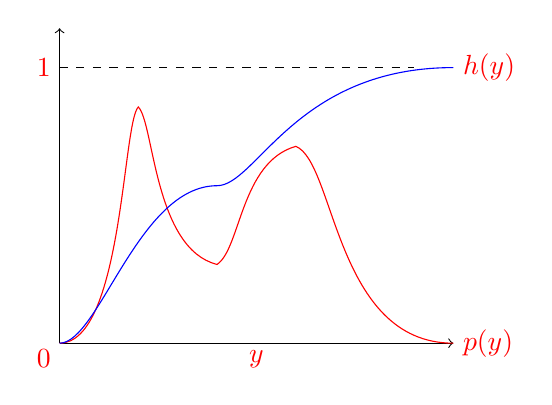
\begin{tikzpicture}
		\draw[->] (0,0) -- (5,0) node at (-0.2,3.5) {$1$};
		\draw[->] (0,0) -- (0,4) node at (-0.2,-0.2){$0$};
		\draw[dashed] (0,3.5) -- (4.5,3.5) node at (2.5,-0.2) {$y$};
		
		\draw[red]  
		(0,0) .. controls (0.8,0) and (0.8,2.8)  ..  (1,3) .. controls (1.2,2.8) and (1.2,1.2) .. (2,1) .. controls (2.3,1.2) and (2.3,2.3) .. (3,2.5) .. controls (3.5,2.3) and (3.5,0) .. (5,0) node[right] {$p(y)$};
		\draw[blue] (0,0) .. controls (0.5,0) and (1,2) .. (2,2) .. controls (2.5,2) and (3,3.5) ..(5,3.5) node[right] {$h(y)$};

	\end{tikzpicture}
\end{center}

考虑指数分布(exponential distribution)
\begin{equation}
	p(y)=\lambda \exp (-\lambda y)
\end{equation}
其中$0\leqslant y \leqslant \infty$。在这种情况下
\begin{equation}
	h(y)=\int_0^y f(y)dy=1-\exp (-\lambda y)
\end{equation}
从而,如果我们将均匀分布的变量$z$使用$y=-\lambda^{-1}\ln (1-z)$进行变换,那么$y$就会服从指数分布。
\begin{equation}
\begin{aligned}
	z&=h(y)=1-\exp (-\lambda y)\\
	y&=h^{-1}(z)\\
	 &\Rightarrow \exp(-\lambda y) = 1-z\\
	 &\Rightarrow -\lambda y = \ln (1-z)\\
	 &\Rightarrow y=-\frac{1}{\lambda}\ln (1-z)
\end{aligned}
\end{equation}

另一种可以应用变换方法的概率分布是柯西分布
\begin{equation}
	p(y)=\frac{1}{\pi}\frac{1}{1+y^2}
\end{equation}
这种情况下,不定积分的反函数可以用$\tan$函数表示。

对于多个变量情形的推广是很容易的,涉及到变量变化的Jacobian行列式,即
\begin{equation}
	p(y_1,\dots,y_M)=p(z_1,\dots,z_M)\bigg| \frac{\partial (z_1,\dots,z_M)}{\partial (y_1,\dots,y_M)}\bigg| 
\end{equation}

作为变换方法的最后一个例子,我们考虑Box-Muller方法,用于生成高斯概率分布的样本。首先我们生成一对均匀分布的随机变量$z_1,z_2\in (-1,1)$,我们可以这样生成:对$(0,1)$上的均匀分布的变量使用$z\to 2z -1$的方式进行变换。接下来,我们丢弃那些不满足$z_1^2+z_2^2\leqslant 1$的点对。这产生出单位圆内部的一个均匀分布,且$p(z_1,z_2)=\frac{1}{\pi}$。然后,对于每对$z_1,z_2$,我们计算 
\begin{flalign}
	y_1&=z_1\left(\frac{-2\ln r^2}{r^2} \right)^{\frac{1}{2}}\\
	y_2&=z_2\left(\frac{-2\ln r^2}{r^2} \right)^{\frac{1}{2}}
\end{flalign}
其中$r^2=z_1^2+z_2^2$。这样,$y_1$和$y_2$的联合概率分布为
\begin{equation}
	\begin{aligned}
		p(y_1,y_2)&=p(z_1,z_2)\bigg|\frac{\partial (z_1,z_2)}{\partial (y_1,y_2)} \bigg|\\
		&=\left[\frac{1}{\sqrt{2\pi}}\exp \left(\frac{-y_1^2}{2} \right) \right]\left[\frac{1}{\sqrt{2\pi}}\exp \left(\frac{-y_1^2}{2}\right) \right]
	\end{aligned}
\end{equation}
因此$y_1$和$y_2$是独立的,有每个都服从高斯分布,均值为零,方差为1。

\textbf{推导过程:}(Box-Muller变换原理)
\begin{enumerate}
	\item 目标
	\begin{equation}
	\begin{aligned}
		p(y_1,y_2)&=\left[\frac{1}{\sqrt{2\pi}}\exp \left(\frac{-y_1^2}{2} \right) \right]\left[\frac{1}{\sqrt{2\pi}}\exp \left(\frac{-y_1^2}{2}\right) \right]\\
		&=\frac{1}{2\pi}\exp \left(-\frac{y_1^2+y_2^2}{2} \right)
	\end{aligned}
	\end{equation}
	做极坐标变换,则$y_1=R\cos \theta,y_2=R\sin \theta$,则有
	\begin{equation}
		\frac{1}{2\pi}\exp \left(-\frac{y_1^2+y_2^2}{2} \right)=\frac{1}{2\pi}\exp \left(-\frac{R^2}{2} \right)
	\end{equation}
	可以看到这个结果可以看成是两个概率分布的密度函数的乘积,其中一个可以看成是$[0,2\pi]$上均匀分布,将其转换为标准均匀分布则有$\theta \sim U(0,2\pi)=2\pi z_1$,因为($z_1,z_2\sim U(0,1)$)。
	\item 求$h(y_1,y_2)$
	\begin{equation}
		\begin{aligned}
			z&=P(R\leqslant r)\\
			 &=\int_0^{2\pi} d\theta\int_0^r \frac{1}{2\pi}\exp \left(-\frac{\rho^2}{2} \right)\rho d\rho\\
			 &=-\exp\left(\frac{-\rho^2}{2}\right)\bigg|_0^r \\
			 &=-\exp \left(-\frac{r^2}{2}\right)+1
		\end{aligned}
	\end{equation}
	其中$r^2=z_1^2+z_2^2$。
	\item 求$y1,y2$
	\begin{equation}
		\begin{aligned}
			R&=h^{-1}(z)\\
			&=\sqrt{-2\ln (1-z)}
		\end{aligned}
	\end{equation}
	这里是二维联合分布,因此
	\begin{equation}
		\begin{aligned}
			y_1&=R\cos \theta = \frac{z_1}{r} \sqrt{-2\ln (r^2)}\\
			y_2&=R\sin \theta = \frac{z_2}{r} \sqrt{-2\ln (r^2)}
		\end{aligned}
	\end{equation}
\end{enumerate}

显然,变换方法依赖于它能够进行计算所需的概率分布,并且能够求所需的概率分布的不定积分的反函数。这样的计算只对于一些非常有限的简单的概率分布可行,因此我们必须寻找一些更加一般的方法。这里,我们考虑两种方法,即拒绝采样(rejection sampling)和重要采样(importance sampling)。虽然这些方法主要限制在单变量概率分布,因此无法直接应用于多维的复杂问题,但是这些方法确定是更一般的方法的重要成分。
\subsection*{拒绝采样}
拒绝采样框架使得我们能够在满足某些限制条件的情况下,从相对复杂的概率分布中采样。首先,我们考虑单变量分布,然后接下来讨论对于多维情形的推广。

假设我们希望从$p(\boldsymbol{z})$中采样,这个概率分布不是我们目前为止讨论过的简单的标准的概率分布中的一个,从而直接从$p(\boldsymbol{z})$中采样是很困难的。此外,我们假设我们能够很容易地计算对于任意给定的$\boldsymbol{z}$值的$p(\boldsymbol{z})$(不考虑归一化常数$Z$),即
\begin{equation}
	p(z)=\frac{1}{Z_p}\tilde{p}(z)
\end{equation}
其中$\tilde{p}(z)$可以很容易地计算,但是$Z_p$未知。

为了应用拒绝采样方法,我们需要一些简单的概率分布$q(z)$,有时被称为提议分布(proposal distribution),并且我们已经可以从提议分布中进行采样。接下来,我们引入一个常数k,它的值的选择满足下面的性质:对所有的z值,都有$kq(z)\geqslant \tilde{p}(z)$。函数$kq(z)$被称为比较函数。

拒绝采样器的每个步骤涉及到生成两个随机数。首先,我们从概率分布$q(z)$中生成一个数$z_0$。接下来,我们在区间$[0,kq(z)]$上的均匀分布中生成一个数$u_0$。这对随机数在函数$kq(z)$的曲线下方是均匀分布。最后,如果$u_0>\tilde{p}(z_0)$,那么样本被拒绝,否则$u_0$被保留。因此对应的$z$值服从概率分布$p(z)$,正如我们所需的那样。
\begin{center}
	\begin{tikzpicture}
		\filldraw[gray!50,line width=2] (-3,1) .. controls (-1,1) and (0,4).. (1,4) .. controls (2,4) and (3,1).. (5,1);
		\draw[pattern=north west lines,gray!50] (-3,0.1) rectangle (5,1);
		
		\filldraw[line width=2,draw=red,white] (-1.5,0.1) .. controls (-1,0.1) and (-0.7,2).. (0,2) .. controls (0.3,2) and (0.7,1).. (1,1).. controls (1.3,1) and (1.5,3).. (2,3) .. controls (2.5,3) and (2.5,0.1).. (4,0.1);
		
		\draw[->] (-3,0) -- (5,0) node[below] at (0,0){$z_0$};
		\draw[->] (0,0) -- (0,4);
		
		\node[fill,draw,circle,inner sep=0.5mm,black,label=left:$u_0$] at (0,1) {};
		\node[fill,draw,circle,inner sep=0.5mm,black,label=left:$kq(z_0)$] at (0,3.3) {};
		\node[label=left:$\tilde{p}(z)$] at (3,1) {};
		\node[black,label=left:$kq(z)$] at (3,4) {};
	\end{tikzpicture}
\end{center}
$z$的原始值从概率分布$q(z)$中生成,这些样本之后被接受的概率为$\frac{\tilde{p}(z)}{kq(z)}$,因此一个样本会被接受的概率为
\begin{equation}
	\begin{aligned}
		p(\text{接受})&=\int \left\{\frac{\tilde{p}(z)}{kq(z)} \right\}q(z)dz\\
		&=\frac{1}{k}\int \tilde{p}(z)dz
	\end{aligned}
\end{equation}
因此,被这种方法拒绝的点的比例依赖于曲线$kq(z)$下方的未归一化概率分布$\tilde{p}(z)$的面积的比例。于是,我们看到,常数k应该尽量小,同时满足下面的限制条件:$kq(z)$一定处处不小于$\tilde{p}(z)$。
\subsection*{可调节的拒绝采样}
在许多我们希望应用拒绝采样的情形中,确定概率分布$q(z)$的一个合适的解析形式是很困难的。另一种确定其函数形式的方法是基于概率分布$p(z)$的值直接构建函数形式。

对于$p(z)$是对数凹函数的情形,即$\ln p(z)$的导数是$z$的单调非增函数时,界限函数的构建是相当简单的。函数$\ln p(z)$和它的切线在某些初始的格点处进行计算,生成的切线的交点被用于构建界限函数。接下来,我们从界限分布中抽取一个样本值。因为界限函数的对数是一系列的线性函数,因此界限函数本身由一个分段指数分布组成,形式为
\begin{equation}
	q(z)=k_i\lambda_i\exp \{-\lambda_i(z-z_i) \}\quad \hat{z}_{i-1,i}<z\leqslant \hat{z}_{i,i+1}
\end{equation}
其中$\hat{z}_{i-1,i}$是在点$z_{i-1}$和$z_i$处的切线的交点,$\lambda_i$是切线在$z_i$处的斜率,$k_i$表示对应的偏移量。一旦一个样本点被抽取完毕,我们就可以应用通常的拒绝准则了。如果样本被接受,那么它就是所求的概率分布中的一个样本。然而,如果样本被拒绝,那么它被并入的集合中,计算出一条新的切线,从而界限函数被优化。随着格点数量的增加,界限函数对所求的概率分布的近似效果逐渐变好,拒绝的概率就会减小。

这个算法存在一种变体,这种变体中不用计算导数。可调节的拒绝采样的框架也可以扩展到不是对数凹函数的概率分布中,只需将每个拒绝采样的步骤中使用Metropolis-Hasting阶梯函数即可,这就产生了可调节拒绝Metropolis采样(adaptive rejection Metropolis sampling)方法。

显然,对于具有实际价值的拒绝采样来说,我们要求对比函数要接近所求的概率分布,从而拒绝率要保持一个最小值。对于更实际的例子来说,所求的概率分布可能是多峰的,并且具有尖峰,从而找到一个较好的提议分布和比较函数是一件相当困难的事情。此外,接受率随着维度的指数下降是拒绝采样的一个一般特征。虽然拒绝采样在一维或二维空间中是一个有用的方法,但是它不适用于高维空间。然而,对于高维空间中的更加复杂的算法来说,它起着子过程的作用。
\subsection*{重要采样}
想从复杂概率分布中采样的一个主要原因是能够使用公式$\ref{zhongyao}$计算期望。重要采样(importance sampling)的方法提供了直接近似期望的框架,但是它本身并没有提供从概率分布$p(z)$中采样的方法。

公式$\ref{youxian}$给出的期望的有限和近似依赖于能够从概率分布$p(z)$中采样。然而直接从$p(z)$中采样无法完成,但是对于任意给定的$z$值,我们可以很容易地计算$p(z)$。一种简单的计算期望的方法是将$z$空间离散化为均匀的格点,将被积函数使用求和的方式计算,形式为
\begin{equation}
	\mathbb{E}[f]\simeq \sum_{l=1}^{L}p(z^{(l)})f(z^{(l)})
\end{equation}
这种方法的一个明显的问题是求和式中的项的数量随着$z$的维度指数增长。此外,我们感兴趣的概率分布通常将它们的大部分质量限制在$z$空间的一个很小的区域,因此均匀地采样非常低效,因为在高维的问题中,只有非常小的一部分样本会对求和式产生巨大的贡献。我们希望从$p(z)$的值较大的区域中采样,或者理想情况下,从$p(z)f(z)$的值较大的区域中采样。

与拒绝采样的情形相同,重要采样基于的是对提议分布$q(z)$的使用,我们很容易从提议分布中采样。之后,我们可以通过$q(z)$中的样本$\{z^{(l)} \}$的有限和的形式来表示期望
\begin{equation}
	\begin{aligned}
		\mathbb{E}[f]&=\int f(z)p(z)dz\\
		&=\int f(z) \frac{p(z)}{q(z)}q(z)dz\\
		&\simeq \frac{1}{L}\sum_{l=1}^{L}\frac{p(z^{(l)})}{q(z^{(l)})}f(z^{(l)})
	\end{aligned}
\end{equation}
$r_l=\frac{p(z^{(l)})}{q(z^{(l)})}$被称为重要性权重(importance weights),修正了由于从错误的概率分布中采样引入的偏差。注意,与拒绝采样不同,所有生成的样本都被保留。

常见的情形是,概率分布$p(z)$的计算结果没有归一化,即$p(z)=\frac{\tilde{p}(z)}{Z_p}$,其中$\tilde{p}(z)$可以很容易地计算出来,而$Z_p$未知。类似地,我们可能希望使用重要采样分布$q(z)=\frac{\tilde{q}(z)}{Z_q}$,它具有相同的性质。于是我们有
\begin{equation}
	\begin{aligned}
		\mathbb{E}[f]&=\int f(z)p(z)dz\\
		&=\frac{Z_q}{Z_p}\int f(z)\frac{\tilde{p}(z)}{\tilde{q}(z)}q(z)dz\\
		&\simeq \frac{Z_q}{Z_p}\frac{1}{L}\sum_{l=1}^{L}\tilde{r}_l f(z^{(l)})
	\end{aligned}
\end{equation}
其中$\tilde{r}_l=\frac{\tilde{p}(z)}{\tilde{q}(z)}$。我们可以使用同样的样本集合来计算比值$\frac{Z_p}{Z_q}$,结果为
\begin{equation}
	\begin{aligned}
		\frac{Z_p}{Z_q}&=\int \frac{\tilde{p}(z)}{\tilde{q}(z)}q(z)dz\\
		&\simeq \frac{1}{L}\sum_{l=1}^{L}\tilde{r}_l
	\end{aligned}
\end{equation}
因此
\begin{equation}
	\mathbb{E}[f]\simeq \sum_{l=1}^{L}w_lf(z^{(l)})
\end{equation}
其中我们定义
\begin{equation}
	w_l=\frac{\tilde{r}_l}{\sum_m \tilde{r}_m}
\end{equation}
与拒绝采样的情形相同中,重要采样方法的成功严重依赖于采样分布$q(z)$与所求的概率分布$p(z)$的匹配程度。经常出现的情形是$p(z)$变化剧烈,并且大部分的质量集中于$z$空间的一个相对较小的区域中,此时重要权重$\{r_l\}$由几个具有圈套值的权值控制,剩余的权值相对较小。因此,有效的样本集大小会比表面上的样本集大小L小得多。如果没有样本落在$p(z)f(z)$圈套的区域中,那么问题会更加严重。此时,$r_l$和$r_lf(z^{(l)})$的表面上的方差可能很小,即使期望的估计可能错得离谱。因此,重要性采样方法的一个主要的缺点是它具有产生任意错误的结果的可能性,并且这种错误无法检测。这也强调 采样分布$q(z)$的一个关键的要求,即它不应该在$p(z)$可能圈套的区域中取得较小的值或者为零的值。
\subsection*{采样-重要性-重采样}
拒绝采样方法部分依赖于确定常数k的一个合适的值。对于许多对概率分布$p(z)$和$q(z)$来说,确定一个合适的k值是不现实的,因为任意的足够大的k值才能够保证产生所求的分布的上界,但是这会产生相当小的接受率。

与拒绝采样的情形相同,采样-重要性-重采样(sampling-importance-resampling,SIR)方法也使用采样$q(z)$,但是避免了必须确定常数$k$。这个方法有两个阶段,在第一个阶段,L个样本$z^{(1)},\dots,z^{(L)}$从$q(z)$中抽取。然后在第二个阶段,构建权值$w_1,\dots,w_L$。最后,L个样本的第二个集合从离散概率分布$(z^{(1)},\dots,z^{(L)})$中抽取,概率由权值$(w_1,\dots,w_L)$给定。
\subsection*{采样与EM算法}
蒙特卡罗方法除了为贝叶斯框架的直接实现提供了原理,还在频率学家的框架内起着重要的作用,例如寻找最大似然解。特别地,对于EM算法中的E步骤无法解析地计算的模型,采样方法也可以用来近似E步骤。

考虑一个模型,它的隐含变量为$Z$,可见(观测)变量为$X$,参数为$\theta$。在M步骤中关于$\theta$最大化的步骤为完整数据对数似然的期望,形式为
\begin{equation}
	Q(\theta,\theta^{\text{旧}})=\int p(Z|X,\theta^{\text{旧}})\ln p(Z,X|\theta)dZ
\end{equation}
我们可以使用采样的方法来近似这个积分,方法是计算样本$\{Z^{(l)} \}$上的有限和,这些样本是从当前的对后验概率分布$p(Z|X,\theta^{\text{旧}})$的估计中抽取的,即
\begin{equation}
	Q(\theta,\theta^{\text{旧}})\simeq \frac{1}{L}\sum_{l=1}^{L}\ln p(Z^{(l)},X|\theta)
\end{equation}
然后,Q函数在M步骤中使用通常的步骤进行优化。这个步骤被称为蒙特卡罗EM算法(Monte Carlo EM algorithm)。

现在假设我们从最大似然的方法转移到纯粹的贝叶斯方法,其中我们希望从参数向量$\theta$上的后验概率分布中进行采样。原则上,我们希望从联合后验分布$p(\boldsymbol{\theta},\boldsymbol{Z}|\boldsymbol{X})$中抽取样本,但是我们假设这个计算十分困难。进一步地,我们假设从完整数据参数的后验概率分布$p(\boldsymbol{\theta}|\boldsymbol{Z},\boldsymbol{X})$中进行采样相对简单。这就产生了数据增广算法(data augmentation algorithm),它在两个步骤之间交替进行,这两个步骤被称为I步骤(归咎(imputation)步骤,类似于E步骤)和P步骤(后验(posterior)步骤,类似于M步骤)。
\begin{enumerate}
	\item I步骤。我们希望从概率分布$p(\boldsymbol{Z}|\boldsymbol{X})$采样,但是我们不能直接进行。于是,我们注意到下面的关系
	\begin{equation}
		p(\boldsymbol{Z}|\boldsymbol{X})=\int p(\boldsymbol{Z}|\boldsymbol{\theta},\boldsymbol{X})p(\boldsymbol{\theta}|\boldsymbol{X})d\boldsymbol{X}
	\end{equation}
	因此对于$l=1,\dots,L$,我们首先从当前对$p(\boldsymbol{\theta}|\boldsymbol{X})$的估计中抽取样本$\boldsymbol{\theta}^{(l)}$,然后使用这个样本从$p(\boldsymbol{Z}|\boldsymbol{\theta}^{(l)},\boldsymbol{X})$中抽取样本$\boldsymbol{Z}^{(l)}$。
	\item P步骤。给定关系
	\begin{equation}
		p(\boldsymbol{\theta}|\boldsymbol{X})=\int p(\boldsymbol{\theta}|\boldsymbol{Z},\boldsymbol{X})p(\boldsymbol{Z}|\boldsymbol{X})d\boldsymbol{Z}
	\end{equation}
	我们使用从I步骤中得到的样本$\{\boldsymbol{Z}^{(l)} \}$,计算$\boldsymbol{\theta}$上的后验概率分布的修正后的估计,结果为
	\begin{equation}
		p(\boldsymbol{\theta}|\boldsymbol{X})\simeq \frac{1}{L}\sum_{l=1}^{L}p(\boldsymbol{\theta}|\boldsymbol{Z}^{(l)},\boldsymbol{X})
	\end{equation}
	根据假设,在I步骤中从这个近似分布中采样是可行的。
\end{enumerate}

注意,我们对参数$\boldsymbol{\theta}$和隐含变量$\boldsymbol{Z}$进行了区分。从现在开始,我们不进行这种区分,仅仅集中于从给定的后验概率分布中抽取样本的问题。
\section{马尔科夫链蒙特卡罗}
前一节中,我们讨论了计算函数期望的拒绝采样方法和重要采样方法,我们看到在高维空间中,这两种方法具有很大的局限性。因此,我们在本节中讨论一个非常一般的并且强大的框架,被称为马尔可夫链蒙特卡罗(Markov chain Monte Carlo,MCMC),它使得我们可以从一大类概率分布中进行采样,并且可以很好地应对空间维度的增长。

与拒绝采样和重要采样相同,我们再一次从提议分布中采样。但是这次我们记录下当前状态$z^{(\tau)}$,以及依赖于这个当前状态的提议分布$q(z|z^{(\tau)})$,从而样本序列$z^{(1)},z^{(2)},\dots,$组成了一个马尔可夫链。与之前一样,如果我们有$p(z)=\frac{\tilde{p}(z)}{Z_p}$,那么我们会假定对于任意的z值都可以计算$\tilde{p}(z)$,虽然$Z_p$的值可能未知。提议分布本身被选择为足够简单,从而直接采样很容易。在算法的每次迭代中,我们从提议分布中生成一个候选样本$z^*$,然后根据一个恰当的准则接受这个样本。

在基本的Metropolis算法中,我们假定提议分布是对称的,即$q(z_A|z_B)=q(z_B|z_A)$对于所有的$z_A$和$z_B$成立。这样,候选的样本被接受的概率为
\begin{equation}
	A(z^*,z^{(\tau)})=\mathrm{min}\left(1,\frac{\tilde{p}(z^*)}{\tilde{p}(z^{(\tau)})}\right)
\end{equation}
可以这样实现:在单位区间$(0,1)$上的均匀分布中随机选择一个数$u$,然后如果$A(z^*,z^{(\tau)})>u$就接受这个样本。注意,如果从$z^{\tau}$到$z^*$引起了$p(z)$的值的增大,那么这个候选样本当然会被保留。

如果候选样本被接受,那么$z^{(\tau+1)}=z^*$,否则候选样本点$z^*$被丢弃,$z^{(\tau+1)}$被设置为$z^{(\tau)}$,然后从概率分布$q(z|z^{(\tau+1)})$中再次抽取一个候选样本。

通过考察一个具体的例子,即简单的随机游走的例子,我们可以对马尔可夫链蒙特卡罗算法的本质得到更深刻的认识。考虑一个由整数组成的状态空间$z$,概率为
\begin{flalign}
	p(z^{(\tau+1)}&=z^{(\tau)})=0.5\\
	p(z^{(\tau+1)}&=z^{(\tau)}+1)=0.25\\
	p(z^{(\tau+1)}&=z^{(\tau)}-1)=0.25
\end{flalign}
其中$z^{(\tau)}$表示在步骤$\tau$的状态。如果初始状态是$z^{(0)}=0$,那么根据对称性,在时刻$\tau$的期望状态也是零,即$\mathbb{E}[z^{(\tau)}]=0$,类似地很容易看到$\mathbb{E}[(z^{(\tau)})]=\frac{\tau}{2}$。因此,在$\tau$步骤之后,随机游走所经过的平均距离正比于$\tau$的平方根。这个平方根依赖关系是随机游走行为的一个典型性质,表明了随机游走在探索状态空间时是很低效的。设计马尔可夫链蒙特卡罗方法的一个中心目标就是避免随机游走行为。

MCMC方法是使用马尔可夫链的蒙特卡罗积分,其基本思想是:构造一条Markov链使其平稳分布为待估参数的后验分布,通过这条马尔可夫链产生后验分布的样本,并基于马尔可夫链达到平稳分布时的样本(有效样本)进行蒙特卡罗积分。设为某一空间n为产生的总样本数m为链条达到平稳时的样本数则MCMC方法的基本思路可概括为:
\begin{enumerate}
	\item 构造Markov链。构造一条Markov链,使其收敛到平稳分布;
	\item 产生样本。由其中的某一点出发,用(1)中的Markov链进行抽样模拟,产生点序列;
	\item 蒙特卡罗积分。任一函数的期望估计为
\end{enumerate}
在采用MCMC方法时马尔可夫链转移核的构造至关重要,不同的转移核构造方法将产生不同的MCMC方法,当前常用的MCMC方法主要有两种Gibbs抽样和Metropo-Lis-Hastings算法。
\subsection*{马尔可夫链}
在详细讨论MCMC方法之前,仔细研究马尔可夫链的一些一般的性质是很有用的。特别地,我们考察在什么情况下马尔可夫链会收敛到所求的概率分布上。 

如果对于所有的时刻$m$,转移概率都相同,那么这个马尔可夫链被称为同质的(homogeneous)。对于一个特定的变量,边缘概率可以根据前一个变量的边缘概率用链式乘积的方式表示出来,形式为
\begin{equation}
	p(z^{(m+1)})=\sum_{z^{(m)}}p(z^{(m+1)}|z^{(m)})p(z^{(m)})
\end{equation}
对于一个概率分布来说,如果马尔可夫链中的每一步都让这个概率分布保持不变,那么我们说这个概率分布关于这个马尔可夫链是不变的,或者静止的。因此,对于一个转移概率为$T(z^{'},z)$的同质的马尔可夫链来说,如果
\begin{equation}
	p^*(z)=\sum_{z^{'}}T(z^{'},z)p^*(z^{'})
\end{equation}
那么概率分布$p^*(z)$是不变的。注意,一个给定的马尔可夫链可能有多个不变的概率分布。例如,如果转换概率由恒等变换给出,那么任意的概率分布都是不变的。

确保所求的概率分布$p(z)$不变的一个充分(非必要)条件是令转移概率满足细节平衡(detailed balance)性质,定义为
\begin{equation}
	p^*(z)T(z,z^{'})=p^*(z^{'})T(z^{'},z)
\end{equation}
对特定的概率分布$p^*(z)$成立。很容易看到,满足关于特定概率分布的细节平衡性质的转移概率会使得那个概率分布具有不变性,因为 
\begin{equation}
	\sum_{z^{'}}p^*(z^{'})T(z^{'},z)=\sum_{z^{'}}p^*(z)T(z,z^{'})=p^*(z)\sum_{z^{'}}p(z^{'}|z)=p^*(z)
\end{equation}
满足细节平衡性质的马尔可夫链被称为可翻转的(reversible)。

我们的目标是使用马尔可夫链从一个给定的概率分布中采样。如果我们构造一个马尔可夫链使得所求的概率分布是不变的,那么我们就可以达到这个目标。然而,我们还要要求对于$m\to \infty$,概率分布$p(z^{(m)})$收敛到所求的不变的概率分布$p^*(z)$,与初始概率分布$p(z^{(0)})$无关。这种性质被称为各态历经性(ergodicity),这个不变的概率分布被称为均衡(equilibrium)分布。很明显,一个具有各态历经性的马尔可夫链只能有唯一的一个均衡分布。可以证明,同质的马尔可夫链具有各态历经性,只需对不变的概率分布和转移概率做出较弱的限制即可。


\subsection*{Metropolis-Hastings算法}
在算法的步骤$\tau$中,当前状态为$z^{(\tau)}$,我们从概率分布$q_k(z^{(\tau)})$中抽取一个样本$z^*$,然后以概率$A_k(z^*,z^{(\tau)})$接受它,其中
\begin{equation}
	A_k(z^*,z^{(\tau)})=\mathrm{min}\left(1,\frac{\tilde{p}(z^*)q_k(z^{(\tau)}|z^*)}{\tilde{p}(z^{(\tau)})q_k(z^{(\tau)}|z^*)} \right) 
\end{equation}
这里,k标记出可能的转移集合中的成员。与之前一样,接受准则的计算不需要知道概率分布$p(z)=\frac{\tilde{p}(z)}{Z_p}$中的归一化常数$Z_p$。

我们现在证明$p(z)$对于由Metropolis-Hastings算法定义的马尔可夫链是一个不变的概率分布,方法是证明满足细节平衡。我们有
\begin{equation}
	\begin{aligned}
		p(z)q_k(z^{'}|z)A_k(z^{'},z)&=\mathrm{min}(p(z)q_k(z^{'}|z),p(z^{'})q_k(z|z^{'})\\
		&=p(z^{'})q_k(z|z^{'})\mathrm{min}(\frac{p(z)q_k(z^{'}|z)}{p(z^{'})q_k(z|z^{'})},1)\\
		&=p(z^{'})q_k(z|z^{'})A_k(z,z^{'})
	\end{aligned}
\end{equation}
证明完毕。


\section{吉布斯采样}

\section{切片采样}

\section{混合蒙特卡罗算法}
正如我们已经注意到的那样,Metropolis算法的一个主要的局限是它具有随机游走的行为,而在状态空间中遍历的距离与步骤数量只是平方根的关系。仅仅通过增大步长的方式是无法解决这个问题的,因为这会使得拒绝率变高。

本节中,我们介绍一类更加复杂的转移方法。这些方法基于对物理系统的一个类比,能够让系统发生较大的改变,同时让拒绝的概率较低。它适用于连续变量上的概率分布,对于连续变量,我们已经能够计算对数概率关于状态变量的梯度。我们会讨论动态系统框架,然后,我们会解释这个框架如何与Metroplolis算法结合,产生出一个强大的混合蒙特卡罗算法。
\subsection*{动态系统}
\subsection*{混合蒙特卡罗方法}
\section{估计划分函数}

\chapter{连续潜在变量}
我们讨论了具有离散潜在变量的概率模型,例如高斯混合模型。我们现在研究某些潜在变量或者全部潜在变量为连续变量的模型。研究这种模型的一个重要的动机是许多数据集具有下面的性质:数据点几乎全部位于比原始数据空间的维度低得多的流形中。

在实际应用中,数据点不会被精确限制在一个光滑的低维流形中,我们可以将数据点关于流形的偏移看做噪声。这就自然地引出了这种模型的生成式观点,其中我们首先根据某种潜在变量的概率分布在流形中选择一个点,然后通过添加噪声的方式生成观测数据点。噪声服从给定潜在变量下的数据变量的某个条件概率分布。

最简单的连续潜在变量模型对潜在变量和观测变量都作出了高斯分布的假设,并且使用了观测变量对于潜在变量状态的线性高斯依赖关系。这就引出了一个著名的技术——主成分分析(PCA)的概率表示形式,也引出了一个相关的模型,被称为因子分析。

本章中,我们首先介绍标准的、非概率的PCA方法,然后我们会说明,当求解线性高斯潜在变量模型的一种特别形式的最大似然解时,PCA如何自然地产生。这种概率形式的表示方法会带来很多好处,例如在参数估计时可以使用EM算法,对混合PCA模型的推广,以及主成分的数量可以从数据中自动确定的贝叶斯公式。最后,我们简短地讨论潜在变量概念的几个推广,使得潜在变量的概念不局限于线性高斯假设。这种推广包括非高斯潜在变量,它引出了独立成分分析(independent conponent analysis)的框架。这种推广还包括潜在变量与观测变量的关系是非线性关系的模型。
\section{主成分分析}
\section{概率PCA}
前一节讨论的PCA的形式所基于的是将数据线性投影到比原始数据空间维度更低的子空间内。PCA也可以被视为概率潜在变量模型的最大似然解。PCA的这种形式,被称为概率PCA(probabilistic PCA),与传统的PCA相比,会带来如下几个优势。
\begin{itemize}
	\item 概率PCA表示高斯分布的一个限制形式,其中自由参数的数量可以受到限制,同时仍然使得模型能够描述数据集的主要的相关关系。
	\item 我们可以为PCA推导一个EM算法,这个算法在只有几个主要的特征向量需要求出的情况下,计算效率比较高,并且避免了计算数据协方差的中间步骤。
	\item 概率模型与EM的结合使得我们能够处理数据集里缺失值的问题。
	\item 概率PCA混合模型可以用一种有理有据的方式进行形式化,并且可以使用EM算法进行训练。
	\item 概率PCA构成了PCA的贝叶斯方法的基础,其中主子空间的维度可以自动从数据中找到。
	\item 似然函数的存在使得直接与其他的概率密度模型进行对比成为可能。相反,传统的PCA会给接近主子空间的数据点分配一个较低的重建代价,即使这些数据点的位置距离训练数据任意远。
	\item 概率PCA可以被用来对类条件概率密度建模,因此可以应用于分类问题。
	\item 概率PCA模型可以用一种生成式的方式运行,从而可以按照某个概率分布生成样本。
\end{itemize}
这种概率模型形式的PCA由Tipping and Bishop和Roweis独立提出。它与因子分析(factor analysis)密切相关。

概率PCA是线性高斯框架的一个简单的例子,其中所有的边缘概率分布和条件概率分布都是高斯分布。我们可以按照下面的方式建立概率PCA模型。首先显式地引入潜在变量$\boldsymbol{z}$,对应于主成分子空间。接下来我们定义潜在变量上的一个高斯先验分布$p(z)$以及以潜在变量的值为条件,观测变量$\boldsymbol{x}$的高斯条件概率分布$p(\boldsymbol{x}|\boldsymbol{z})$。具体地说,$\boldsymbol{z}$上的先验概率分布是一个零均值单位协方差的高斯分布
\begin{equation}
	p(\boldsymbol{z})=\mathcal{N}(\boldsymbol{z}|0,\boldsymbol{I})
\end{equation}
类似地,以潜在变量$\boldsymbol{z}$的值为条件,观测变量$\boldsymbol{x}$的条件概率分布还是高斯分布,形式为
\begin{equation}
	p(\boldsymbol{x}|\boldsymbol{z})=\mathcal{N}(\boldsymbol{x}|\boldsymbol{W}\boldsymbol{z}+\boldsymbol{\mu},\sigma^2\boldsymbol{I})
\end{equation}
其中$\boldsymbol{x}$的均值是$\boldsymbol{z}$的一个一般的线性函数,由$D\times M$的矩阵$\boldsymbol{W}$和D维向量$\boldsymbol{\mu}$控制。注意,可以关于$\boldsymbol{x}$的各个元素进行分解,换句话说,这是朴素贝叶斯模型的一个例子。

我们可以从生成式的观点看待概率PCA模型,其中观测值的一个采样值通过下面的方式获得:首先为潜在变量选择一个值,然后以这个潜在变量的值为条件,对观测变量采样。具体来说,D维观测变量$\boldsymbol{x}$由M
维潜在变量$\boldsymbol{z}$的一个线性变换附加一个高斯“噪声”定义,即
\begin{equation}
\label{1233}
	\boldsymbol{x}=\boldsymbol{Wz}+\boldsymbol{\mu}+\boldsymbol{\epsilon}
\end{equation}
其中$\boldsymbol{z}$是一个M维高斯潜在变量,$\boldsymbol{\epsilon}$是一个D维零均值高斯分布的噪声变量,协方差为$\sigma^2\boldsymbol{I}$。注意,这个框架基于的是从潜在空间到数据空间的一个映射,这与之前讨论的PCA的传统观点不同。从数据空间到潜在空间的逆映射可以通过使用贝叶斯定理的方式得到。

假设我们希望使用最大似然的方式确定参数$\boldsymbol{W,\mu}$和$\sigma^2$的值。为了写出似然函数的表达式,我们需要观测变量的边缘概率分布$p(\boldsymbol{x})$的表达式。
\begin{equation}
	p(\boldsymbol{x})=\int p(\boldsymbol{x}|\boldsymbol{z})p(\boldsymbol{z})d\boldsymbol{z}
\end{equation}
由于这对应于一个线性高斯模型,因此边缘概率分布还是高斯分布,形式为
\begin{equation}
\label{1235}
	p(\boldsymbol{x})=\mathcal{N}(\boldsymbol{x}|\boldsymbol{\mu,C})
\end{equation}
其中$D\times D$协方差矩阵$C$被定义为
\begin{equation}
	\begin{aligned}
	C&=\mathrm{var}[\boldsymbol{x}]=\mathrm{var}[\boldsymbol{Wz}+\boldsymbol{\mu}+\boldsymbol{\epsilon}]\\
	&=\mathrm{var}[\boldsymbol{Wz}]+\mathrm{var}[\boldsymbol{\epsilon}]\\
	&=\boldsymbol{WIW}^T+\sigma^2\boldsymbol{I}\\
	&=\boldsymbol{WW}^T+\sigma^2\boldsymbol{I}
	\end{aligned}
\end{equation}
我们注意到预测概率分布是高斯分布,然后使用公式$\ref{1233}$计算它的均值和协方差,结果为
\begin{flalign}
	\mathbb{E}[\boldsymbol{x}]&=\mathbb{E}[\boldsymbol{Wz}+\boldsymbol{\mu}+\boldsymbol{\epsilon}]=\boldsymbol{\mu}\\
	\mathrm{var}[\boldsymbol{x}]&=\boldsymbol{WW}^T+\sigma^2\boldsymbol{I}
\end{flalign}
其中我们使用了下面的事实:$\boldsymbol{z}$和$\boldsymbol{\epsilon}$是独立的随机变量,因此非相关。

预测分布$p(\boldsymbol{x})$由参数$\boldsymbol{W,\mu}$和$\sigma^2$控制。然而,这些参数中存在冗余性,对应于潜在空间坐标的旋转。

与预测分布$p(\boldsymbol{x})$一样,我们也需要后验概率分布$p(\boldsymbol{z}|\boldsymbol{x})$,这可以直接使用公式给出的线性高斯模型的结果写出来,结果为
\begin{equation}
	p(\boldsymbol{z}|\boldsymbol{x})=\mathcal{N}(\boldsymbol{z}|\boldsymbol{M}^{-1}\boldsymbol{W}^T(\boldsymbol{x}-\boldsymbol{\mu}),\sigma^2\boldsymbol{M}^{-1})
\end{equation}
其中 
\begin{equation}
	\boldsymbol{M}=\sigma^2\boldsymbol{I}_M+\boldsymbol{W}^T\boldsymbol{W}
\end{equation}
注意,后验均值依赖于$\boldsymbol{x}$,而后验协方差与$\boldsymbol{x}$无关。
\subsection*{最大似然PCA}
我们接下来考虑使用最大似然法确定模型的参数,给定观测数据点的数据点$\boldsymbol{X}=\{\boldsymbol{x}_n\}$,概率PCA模型可以表示为一个有向图。
\begin{center}
	\begin{tikzpicture}[node distance=2cm]
		\tikzstyle{every node} = [color=red]
		
		\node[state] (A) {$Z_n$};
		\node[state,below of=A,fill=gray!25] (B) {$X_n$};
		
		\node[circle,inner sep=0.1cm,fill=red,left of=A,label=left:$\sigma^2$](C){}; 
		\node[circle,inner sep=0.1cm,fill=red,left of=B,label=left:$\boldsymbol{\mu}$](D){}; 
		\node[circle,inner sep=0.1cm,fill=red,right of=B,label=right:$\boldsymbol{W}$](E){}; 
		\node[right of=B,xshift=-1.4cm,yshift=-0.6cm,blue](G) {$N$};
		\node[draw,color=blue,inner sep=0.3cm,rectangle,fit=(A)(B),rounded corners](F){};
		
		\path (A) edge[->] (B)
		(C) edge[->] (B)
		(D) edge[->] (B)
		(E) edge[->] (B);
	\end{tikzpicture}
\end{center}
根据公式$\ref{1235}$,对应的对数似然函数为
\begin{equation}
	\begin{aligned}
		\ln p(\boldsymbol{X}|\boldsymbol{\mu},\boldsymbol{W},\sigma^2)&=\sum_{n=1}^{N}\ln p(\boldsymbol{x}_n|\boldsymbol{\mu},\boldsymbol{W},\sigma^2)\\
		&=-\frac{ND}{2}\ln (2\pi)-\frac{N}{2}\ln |C|-\frac{1}{2}\sum_{n=1}^{N}(\boldsymbol{x}_n-\boldsymbol{\mu})^TC^{-1}(\boldsymbol{x}_n-\boldsymbol{\mu})
	\end{aligned}
\end{equation}
令似然函数关于$\boldsymbol{\mu}$的导数等于零,可以得到预期的结果$\boldsymbol{\mu}=\bar{\boldsymbol{x}}$,代回到似然函数中,我们有
\begin{equation}
\begin{aligned}
	\ln p(\boldsymbol{X}|\boldsymbol{\mu},\boldsymbol{W},\sigma^2)&=-\frac{N}{2}\{D\ln (2\pi)+\ln |C|\}+\frac{N}{2}\mathrm{Tr}\left(C^{-1}\frac{1}{N}\sum_{n=1}^{N}(\boldsymbol{x}_n-\boldsymbol{\mu})^T(\boldsymbol{x}_n-\boldsymbol{\mu}) \right)\\
	&=-\frac{N}{2}\{D\ln (2\pi)+\ln |C|+\mathrm{Tr}(C^{-1}S) \}
\end{aligned}
\end{equation}
其中$S$是协方差矩阵。由于对数似然函数是$\boldsymbol{\mu}$的二次函数,因此解具有唯一的最大值,可以通过计算二阶导数的方式验证这一点。

\begin{proof}迹运算描述Frobenius范数
	
	设$A$是m行n列的矩阵,A的行向量是$\overrightarrow{b}_1^T,\dots,\overrightarrow{b}_m^T$。那么 
	\begin{equation}
		A=\begin{pmatrix}
			\overrightarrow{b}_1^T\\
			\overrightarrow{b}_2^T\\
			\vdots\\
			\overrightarrow{b}_m^T
		\end{pmatrix},\qquad 
		A^T=\begin{pmatrix}
			\overrightarrow{b}_1,
			\overrightarrow{b}_2,
			\dots
			\overrightarrow{b}_m^T
		\end{pmatrix}
	\end{equation}
	\begin{equation}
		AA^T=\begin{pmatrix}
			\overrightarrow{b}_1^T\\
			\overrightarrow{b}_2^T\\
			\vdots\\
			\overrightarrow{b}_m^T
		\end{pmatrix}\begin{pmatrix}
			\overrightarrow{b}_1,
			\overrightarrow{b}_2,
			\dots
			\overrightarrow{b}_m^T
		\end{pmatrix}=\begin{pmatrix}
			\overrightarrow{b}_1^T\overrightarrow{b}_1&\overrightarrow{b}_1^T\overrightarrow{b}_2&
			\dots&
			\overrightarrow{b}_1^T\overrightarrow{b}_m\\
			\overrightarrow{b}_2^T\overrightarrow{b}_1&\overrightarrow{b}_2^T\overrightarrow{b}_2&
			\dots&
			\overrightarrow{b}_2^T\overrightarrow{b}_m\\
			\vdots&\vdots&\ddots&\vdots\\
			\overrightarrow{b}_m^T\overrightarrow{b}_1&\overrightarrow{b}_m^T\overrightarrow{b}_2&
			\dots&
			\overrightarrow{b}_m^T\overrightarrow{b}_m			
		\end{pmatrix}
	\end{equation}
	因为迹运算返回的是矩阵对角线元素的和,所以:
	\begin{equation}
		\mathrm{Tr}(AA^T)=\sum_{i=1}^{m}\overrightarrow{b}_i^T\overrightarrow{b}_i
	\end{equation}
	$\overrightarrow{b}_i^T$是矩阵A的第i行。$\overrightarrow{b}_i^T=(A_{i,1},\dots,A_{i,n})$,$\overrightarrow{b}_i^T\overrightarrow{b}_i$是矩阵A第i行行向量的内积。那么
	\begin{equation}
		\overrightarrow{b}_i^T\overrightarrow{b}_i=\sum_{j=1}^{n}A_{ij}^2
	\end{equation}
	推出
	\begin{equation}
		\mathrm{Tr}(AA^T)=\sum_{i=1}^{m}\sum_{j=1}^{n}A_{ij}^2
	\end{equation}
	即
	\begin{equation}
		\lVert A \rVert_F=\sqrt{\sum_{i=1}^{m}\sum_{j=1}^{n}A_{ij}^2}=\sqrt{\mathrm{Tr}(AA^T)}
	\end{equation}
\end{proof}

令$F=-\ln p(\boldsymbol{X}|\boldsymbol{\mu},\boldsymbol{W},\sigma^2)$(忽略掉常数项)。
\begin{equation}
	F=\ln |C|-\mathrm{Tr}(C^{-1}S)
\end{equation}
\begin{enumerate}
	\item 令 $\frac{\mathrm{d}F}{\mathrm{d}\boldsymbol{W}}=0$求$\boldsymbol{W}$
	\begin{equation}
		\begin{aligned}
			\mathrm{d}F&=\mathrm{d}\ln |\boldsymbol{C}| +\mathrm{d}\mathrm{Tr}(\boldsymbol{C}^{-1}\boldsymbol{S})\\
			&=\mathrm{Tr}(\boldsymbol{C}^{-1}\mathrm{d}C)+\mathrm{Tr}(\mathrm{d}C^{-1}\boldsymbol{S})\\
			&=\mathrm{Tr}(\boldsymbol{C}^{-1}\mathrm{d}C)-\mathrm{Tr}(\boldsymbol{C}^{-1}\mathrm{d}\boldsymbol{C}\boldsymbol{C}^{-1}\boldsymbol{S})\\
			&=\mathrm{Tr}(\boldsymbol{C}^{-1}(\mathrm{d}\boldsymbol{WW}^T+\boldsymbol{W}\mathrm{d}\boldsymbol{W}^T))-\mathrm{Tr}(\boldsymbol{C}^{-1}(\mathrm{d}\boldsymbol{WW}^T+\boldsymbol{W}\mathrm{d}\boldsymbol{W}^T)\boldsymbol{C}^{-1}\boldsymbol{S})
		\end{aligned}
	\end{equation}
	根据迹的性质,有
	\begin{equation}
		\mathrm{Tr}(\boldsymbol{C}^{-1}\mathrm{d}\boldsymbol{WW}^T)=\mathrm{Tr}(\boldsymbol{W}\mathrm{d}\boldsymbol{W}^T\boldsymbol{C}^{-1})=\mathrm{Tr}(\boldsymbol{C}^{-1}\boldsymbol{W}\mathrm{d}\boldsymbol{W}^T)
	\end{equation}
	代入上式中,有
	\begin{equation}
		\begin{aligned}
			\mathrm{d}F&=2\mathrm{Tr}(\boldsymbol{C}^{-1}\boldsymbol{W}\mathrm{d}\boldsymbol{W}^T)-2\mathrm{Tr}(\boldsymbol{C}^{-1}\boldsymbol{SC}^{-1}\boldsymbol{W}\mathrm{d}\boldsymbol{W}^T)\\
			&=2\mathrm{Tr}[(\boldsymbol{C}^{-1}\boldsymbol{W}-\boldsymbol{C}^{-1}\boldsymbol{SC}^{-1}\boldsymbol{W})\mathrm{d}\boldsymbol{W}^T]
		\end{aligned}
	\end{equation}
	因此,
	\begin{equation}
		\frac{1}{2}\frac{\mathrm{d}F}{\mathrm{d}\boldsymbol{W}}=\boldsymbol{C}^{-1}\boldsymbol{W}-\boldsymbol{C}^{-1}\boldsymbol{SC}^{-1}\boldsymbol{W}
	\end{equation}
	令$\frac{\mathrm{d}F}{\mathrm{d}\boldsymbol{W}}=0$,可求得
	\begin{equation}
	\begin{aligned}
		\boldsymbol{W}&=\boldsymbol{SC}^{-1}\boldsymbol{W}\\
		&=\boldsymbol{S}(\sigma^2\boldsymbol{I}_D+\boldsymbol{WW}^T)^{-1}\boldsymbol{W}\\
		&=\boldsymbol{S}\boldsymbol{W}(\sigma^2\boldsymbol{I}_M+\boldsymbol{W}^T\boldsymbol{W})^{-1}
	\end{aligned}
	\end{equation}
	对$\boldsymbol{W}^T\boldsymbol{W}=\boldsymbol{V}\Lambda \boldsymbol{V}^T$作分解,代入有
	\begin{equation}
		\begin{aligned}
			&\boldsymbol{S}\boldsymbol{W}(\boldsymbol{V}\sigma^2\boldsymbol{I}_M\boldsymbol{V}^T+\boldsymbol{V}\Lambda \boldsymbol{V}^T)^{-1}=\boldsymbol{W}\\
			&\Rightarrow\boldsymbol{S}\boldsymbol{W}{(\boldsymbol{V}^T)}^{-1}(\sigma^2\boldsymbol{I}_M+\Lambda )^{-1}\boldsymbol{V}^{-1}=\boldsymbol{W}\\
			&\Rightarrow\boldsymbol{S}\boldsymbol{W}\boldsymbol{V}(\sigma^2\boldsymbol{I}_M+\Lambda )^{-1}=\boldsymbol{W}\boldsymbol{V}
		\end{aligned}
	\end{equation}
	对$\boldsymbol{WV}$正交化,有
	\begin{equation}
		\Lambda^{-\frac{1}{2}}\boldsymbol{V}^T\boldsymbol{W}^T\boldsymbol{W}\boldsymbol{V}\Lambda^{-\frac{1}{2}}=\Lambda^{-\frac{1}{2}}\boldsymbol{V}^T\boldsymbol{V}\Lambda \boldsymbol{V}^T\boldsymbol{V}\Lambda^{-\frac{1}{2}}=\boldsymbol{I}
	\end{equation}
	因此,我们有
	\begin{equation}
		\boldsymbol{S}\boldsymbol{W}\boldsymbol{V}\Lambda^{-\frac{1}{2}}=\boldsymbol{W}\boldsymbol{V}\Lambda^{-\frac{1}{2}}(\sigma^2\boldsymbol{I}+\Lambda )
	\end{equation}
	令$U_M=\boldsymbol{WV\Lambda}^{-\frac{1}{2}},L_M=\sigma^2\boldsymbol{I}_M+\Lambda$,我们有
	\begin{equation}
		\begin{aligned}
			\boldsymbol{S}U_M&=U_ML_M\\
			\Rightarrow \boldsymbol{W}_{ML}&=U_M\Lambda^{\frac{1}{2}}\boldsymbol{V}^T= U_M(L_M-\sigma^2\boldsymbol{I}_M)^{\frac{1}{2}}\boldsymbol{V}^T
		\end{aligned}
	\end{equation}
	
	
	\item 令$\frac{\mathrm{d}F}{\mathrm{d}\sigma^2}=0$求$\sigma^2$
	
	\begin{equation}
		\begin{aligned}
			\mathrm{d}F&=\mathrm{Tr}(\boldsymbol{C}^{-1}\mathrm{d}\sigma^2\boldsymbol{I})-\mathrm{Tr}(\boldsymbol{C}^{-1}\mathrm{d}\sigma^2\boldsymbol{C}^{-1}\boldsymbol{S})\\
			&=[\mathrm{Tr}(\boldsymbol{C}^{-1})-\mathrm{Tr}(\boldsymbol{C}^{-1}\boldsymbol{S}\boldsymbol{C}^{-1})]\mathrm{d}\sigma^2
		\end{aligned}
	\end{equation}
	令
	\begin{equation}
		\frac{\mathrm{d}F}{\mathrm{d}\sigma^2}=\mathrm{Tr}(\boldsymbol{C}^{-1}-\boldsymbol{C}^{-1}\boldsymbol{S}\boldsymbol{C}^{-1})=0
	\end{equation}
	计算$\boldsymbol{C}^{-1}$
	\begin{equation}
		\boldsymbol{C}^{-1}=(\sigma^2\boldsymbol{I}_D+\boldsymbol{WW}^T)^{-1}=\sigma^{-2}\boldsymbol{I}_D-\sigma^{-2}\boldsymbol{W}(\sigma^2\boldsymbol{I}_M+\boldsymbol{W}^T\boldsymbol{W})^{-1}\boldsymbol{W}^T
	\end{equation}
	等式两边同乘$\boldsymbol{S}$有
	\begin{equation}
		\begin{aligned}
			\boldsymbol{S}\boldsymbol{C}^{-1}&=\sigma^{-2}\boldsymbol{S}-\sigma^{-2}\boldsymbol{S}\boldsymbol{W}(\sigma^2\boldsymbol{I}_M+\boldsymbol{W}^T\boldsymbol{W})^{-1}\boldsymbol{W}^T\\
			&=\sigma^{-2}\boldsymbol{S}-\sigma^{-2}\boldsymbol{WW}^T\quad (\text{因为}\boldsymbol{S}\boldsymbol{W}(\sigma^2\boldsymbol{I}_M+\boldsymbol{W}^T\boldsymbol{W})^{-1}=\boldsymbol{W})
		\end{aligned}
	\end{equation}
	代入上式中,有
	\begin{equation}
	\begin{aligned}
		\boldsymbol{C}^{-1}\boldsymbol{S}\boldsymbol{C}^{-1}-\boldsymbol{C}^{-1}&=\boldsymbol{C}^{-1}\sigma^{-2}\boldsymbol{S}-\boldsymbol{C}^{-1}\sigma^{-2}\boldsymbol{WW}^T-\boldsymbol{C}^{-1}\\
		&=\sigma^{-2}\boldsymbol{C}^{-1}\boldsymbol{S}-\boldsymbol{C}^{-1}\sigma^{-2}\boldsymbol{WW}^T-\boldsymbol{C}^{-1}\\
		&=\sigma^{-2}(\sigma^{-2}\boldsymbol{S}-\sigma^{-2}\boldsymbol{WW}^T)-\boldsymbol{C}^{-1}\sigma^{-2}\boldsymbol{WW}^T-\boldsymbol{C}^{-1}\\
		&=\sigma^{-2}(\sigma^{-2}\boldsymbol{S}-\sigma^{-2}\boldsymbol{WW}^T)-\sigma^{-2}\boldsymbol{C}^{-1}(\boldsymbol{C}-\sigma^2\boldsymbol{I}_D)-\boldsymbol{C}^{-1}\\
		&=\sigma^{-2}(\sigma^{-2}\boldsymbol{S}-\sigma^{-2}\boldsymbol{WW}^T)-\sigma^{-2}\boldsymbol{I_D}\\
		&=\sigma^{-4}\boldsymbol{S}-\sigma^{-4}\boldsymbol{WW}^T-\sigma^{-2}\boldsymbol{I}_D\\
	\end{aligned}
	\end{equation}
	求得
	\begin{equation}
		\begin{aligned}
			\frac{\mathrm{d}F}{\mathrm{d}\sigma^2}=\mathrm{Tr}(\boldsymbol{C}^{-1}-\boldsymbol{C}^{-1}\boldsymbol{S}\boldsymbol{C}^{-1})=\sigma^{-4}\mathrm{Tr}(\boldsymbol{S}-\boldsymbol{WW}^T-\sigma^2\boldsymbol{I}_D)=0
		\end{aligned}
	\end{equation}
	我们有
	\begin{equation}
		\begin{aligned}
			\sigma^2\mathrm{Tr}(\boldsymbol{I}_D)&=\mathrm{Tr}(\boldsymbol{S})-\mathrm{Tr}(\boldsymbol{W}^T\boldsymbol{W})\\
			D\sigma^2&=\mathrm{Tr}(\boldsymbol{S})-\mathrm{Tr}(L-\sigma^2\boldsymbol{I}_M)\\
			&=\mathrm{Tr}(\boldsymbol{S})-\mathrm{Tr}(L_M)+M\sigma^2\\
			(D-M)\sigma^2&=\mathrm{Tr}(\boldsymbol{S})-\mathrm{Tr}(L_M)\\
			\sigma^2&=\frac{\mathrm{Tr}(\boldsymbol{S})-\mathrm{Tr}(L_M)}{D-M}\\
			&=\frac{1}{D-M}\sum_{i=M+1}^{D}\lambda_i
		\end{aligned}
	\end{equation}
\end{enumerate}
总结一下,
\begin{flalign}
	\boldsymbol{W}_{ML}&=U_M(L_M-\sigma^2\boldsymbol{I}_M)^{\frac{1}{2}}\boldsymbol{V}^T\\
	\sigma_{ML}^2&=\frac{1}{D-M}\sum_{i=M+1}^{D}\lambda_i
\end{flalign}
传统的PCA通常的形式是D维空间的数据点在M维线性子空间上的投影。然而,概率PCA可以很自然地表示为从潜在空间到数据空间的映射,由公式$\ref{1233}$给出。对于数据可视化和数据压缩之类的应用,我们可以使用贝叶斯定理将这个映射取逆。这样,任何在数据空间中的点$\boldsymbol{x}$都可以使用潜在空间中的后验均值和方差进行概括。最后,我们注意到,概率PCA模型在定义多元高斯分布时具有重要的作用,其中自由度的数量(即独立参数的数量)可以进行控制,同时仍然使得模型能够描述数据中的主要的相关关系。
\subsection*{用于PCA的EM算法}
概率PCA模型可以根据连续潜在空间$\boldsymbol{z}$上的积分或求和来表示,其中对于每个数据点$\boldsymbol{x}_n$,都存在一个对应的潜在变量$\boldsymbol{z}_n$。于是,我们可以使用EM算法来找到模型参数。这看起来似乎相当没有意义,因为我们已经得到了最大似然参数值的一个精确的解析解。然而,在高维空间中,使用迭代的EM算法而不是直接计算样本协方差矩阵可能会有一些计算上的优势。这个EM的求解步骤也可以推广到因子分析模型中,那里不存在解析解。最后,它使得我们可以用一种有理有据的方式处理缺失的数据。

我们可以使用一般的EM框架来推导用于概率PCA的EM算法。因此,我们写出完整数据对数似然函数,然后关于使用旧的参数值计算的潜在变量的后验概率分布求期望。最大化完整数据对数似然函数的期望就会产生新的参数值。因为我们假定数据点是独立的,因此完整数据对数似然函数的形式为
\begin{equation}
	L_c=\ln p(\boldsymbol{X},\boldsymbol{Z}|\boldsymbol{\mu},\boldsymbol{W},\sigma^2)=\sum_{n=1}^{N}\{\ln p(\boldsymbol{x}_n|\boldsymbol{z}_n)+\ln p(\boldsymbol{z}_n) \}
\end{equation}
这里,$\ln p(\boldsymbol{x}_n,\boldsymbol{z_n})$是
\begin{equation}
	\begin{aligned}
		\ln p(\boldsymbol{x}_n,\boldsymbol{z_n})&=\ln[p(\boldsymbol{x}_n|\boldsymbol{z}_n)p(\boldsymbol{z}_n)]\\
		&=\ln \left[\frac{1}{(2\pi)^{\frac{D}{2}}\sigma^D}\exp (-\frac{1}{\sigma^2}\lVert \boldsymbol{x}_n-\boldsymbol{\mu}-\boldsymbol{Wz}_n\rVert^2)\exp(-\frac{1}{2}\lVert\boldsymbol{z}_n\rVert^2) \right]\\
		&=-\frac{D}{2}\ln \sigma^2-\frac{1}{\sigma^2}\lVert \boldsymbol{x}_n-\boldsymbol{\mu}-\boldsymbol{Wz}_n\rVert^2-\frac{1}{2}\lVert\boldsymbol{z}_n\rVert^2\quad (\text{忽略了常系数})\\
		&=-\frac{D}{2}\ln \sigma^2-\frac{1}{\sigma^2}\lVert \boldsymbol{x}_n-\boldsymbol{\mu}\rVert^2-\frac{1}{\sigma^2}\lVert\boldsymbol{Wz}_n\rVert^2+\frac{1}{\sigma^2}(\boldsymbol{x}_n-\boldsymbol{\mu})^T(\boldsymbol{Wz}_n)-\frac{1}{2}\lVert\boldsymbol{z}_n\rVert^2
	\end{aligned}
\end{equation}
\begin{enumerate}
	\item E-步:$\boldsymbol{\theta}=(\sigma^2,\boldsymbol{W})$,求$L_c$关于$p(\boldsymbol{z}_n|\boldsymbol{\theta})$的期望
	
	\begin{equation}
		\begin{aligned}
			Q(\boldsymbol{\theta}|\boldsymbol{\theta}^{(t)})&=\sum_{n=1}^{N}\int (\ln p(\boldsymbol{x}_n,\boldsymbol{z}_n))p(\boldsymbol{z}_n|\boldsymbol{x}_n,\boldsymbol{\theta}^{(t)})\mathrm{d}\boldsymbol{z}_n\\
			&=\sum_{n=1}^{N}\left\{-\int \frac{D}{2}\ln \sigma^2p(\boldsymbol{z}_n|\theta^{(t)})\mathrm{d}\boldsymbol{z}_n\right.\\
			&\ \ -\int \frac{1}{2\sigma^2}\lVert \boldsymbol{x}_n-\boldsymbol{\mu}\rVert^2p(\boldsymbol{z}_n|\boldsymbol{x}_n,\boldsymbol{\theta}^{(t)})\mathrm{d}\boldsymbol{z}_n\\
			&\ \ -\int \frac{1}{2\sigma^2}\lVert \boldsymbol{Wz}_n\rVert^2p(\boldsymbol{z}_n|\boldsymbol{x}_n,\boldsymbol{\theta}^{(t)})\mathrm{d}\boldsymbol{z}_n\\
			&\ \ -\int \frac{1}{\sigma^2}(\boldsymbol{x}_n-\boldsymbol{\mu})^T(\boldsymbol{Wz}_n)p(\boldsymbol{z}_n|\boldsymbol{x}_n,\boldsymbol{\theta}^{(t)})\mathrm{d}\boldsymbol{z}_n\\
			&\ \ \left.-\int \frac{1}{2}\lVert \boldsymbol{z}_n\rVert^2p(\boldsymbol{z}_n|\boldsymbol{x}_n,\boldsymbol{\theta}^{(t)})\mathrm{d}\boldsymbol{z}_n\right\}\\
			&=-\frac{ND}{2}\ln \sigma^2-\frac{N}{2\sigma^2}\mathrm{Tr}(\boldsymbol{S})\\
			&\ \ -\sum_{n=1}^{N}\int \left[\frac{1}{2\sigma^2}\lVert\boldsymbol{Wz}_n\rVert^2-\frac{1}{\sigma^2}(\boldsymbol{x}_n-\boldsymbol{\mu})^T(\boldsymbol{Wz}_n)+\frac{1}{2}\lVert\boldsymbol{z}_n\rVert^2 \right]p(\boldsymbol{z}_n|\boldsymbol{x}_n,\boldsymbol{\theta}^{(t)})\mathrm{d}\boldsymbol{z}_n
		\end{aligned}
	\end{equation}
	其中我们用到了
	\begin{equation}
		\mathrm{Tr}(\boldsymbol{S})=\frac{1}{N}\sum_{n=1}^{N}\left((\boldsymbol{x}_n-\boldsymbol{\mu})(\boldsymbol{x}_n-\boldsymbol{\mu})^T\right)
	\end{equation}
	我们定义
	\begin{equation}
		\langle\boldsymbol{z}_n\rangle=\int \boldsymbol{z}_np(\boldsymbol{z}_n|\boldsymbol{x}_n,\boldsymbol{\theta}^{(t)})\mathrm{d}\boldsymbol{z}_n=\boldsymbol{M}^{-1}_{(t)}\boldsymbol{W}_{(t)}^T(\boldsymbol{x}_n-\boldsymbol{\mu})
	\end{equation}
	因为$		(\boldsymbol{z}|\boldsymbol{x}-\boldsymbol{\mu})\sim \mathcal{N}(\boldsymbol{M}^{-1}\boldsymbol{W}^T(\boldsymbol{x}_n-\boldsymbol{\mu}),\sigma^2\boldsymbol{M}^{-1}$,这里$\boldsymbol{M}=\sigma^2\boldsymbol{I}_M+\boldsymbol{W}^T\boldsymbol{W})$
	\begin{equation}
		\langle \boldsymbol{z}_n,\boldsymbol{z}_n^T\rangle=\int \boldsymbol{z}_n\boldsymbol{z}_n^Tp(\boldsymbol{z}_n|\boldsymbol{x}_n,\boldsymbol{\theta}^{(t)})\mathrm{d}\boldsymbol{z}_n=\sigma_{(t)}^2\boldsymbol{M}_{(t)}^{-1}+\langle\boldsymbol{z}_n\rangle\langle\boldsymbol{z}_n\rangle^T
	\end{equation}
	因为
	\begin{equation}
		\mathrm{Cov}(\boldsymbol{z}_n)=\mathbb{E}(\boldsymbol{z}_n\boldsymbol{z}_n^T)-\mathbb{E}(\boldsymbol{z}_n)\mathbb{E}(\boldsymbol{z}_n^T)
	\end{equation}
	因此,$Q(\boldsymbol{\theta}|\boldsymbol{\theta}^{(t)})$为
	\begin{equation}
	\begin{aligned}
		Q(\boldsymbol{\theta}|\boldsymbol{\theta}^{(t)})&=-\frac{ND}{2}\ln \sigma^2-\frac{N}{2\sigma^2}\mathrm{Tr}(\boldsymbol{S})\\
		&-\sum_{n=1}^{N}\left\{\frac{1}{2\sigma^2}\mathrm{Tr}(\boldsymbol{W}^T\boldsymbol{W}\langle \boldsymbol{z}_n,\boldsymbol{z}_n^T\rangle)-\frac{1}{\sigma^2}(\boldsymbol{x}_n-\boldsymbol{\mu})^T\boldsymbol{W}\langle\boldsymbol{z}_n\rangle+\frac{1}{2}\mathrm{Tr}(\langle \boldsymbol{z}_n,\boldsymbol{z}_n^T\rangle) \right\}
	\end{aligned}
	\end{equation}
	\item M-步:最大化$Q(\boldsymbol{\theta}|\boldsymbol{\theta}^{(t)})$
	\begin{enumerate}[(a)]
		\item 
		\begin{equation}
			\begin{aligned}
				&\frac{\mathrm{d}Q}{\mathrm{d}\boldsymbol{W}}=\frac{1}{\sigma^2}\sum_{n=1}^{N}(\boldsymbol{x}_n-\boldsymbol{\mu})\langle \boldsymbol{z}_n^T\rangle -\frac{1}{\sigma^2}\sum_{n=1}^{N}\boldsymbol{W}\langle \boldsymbol{z}_n,\boldsymbol{z}_n^T\rangle =0\\
				\Rightarrow&\boldsymbol{W}\sum_{n=1}^{N}\langle \boldsymbol{z}_n,\boldsymbol{z}_n^T\rangle =\sum_{n=1}^{N}(\boldsymbol{x}_n-\boldsymbol{\mu})\langle \boldsymbol{z}_n^T\rangle\\
				\Rightarrow&\boldsymbol{W}^{(t+1)}=\left(\sum_{n=1}^{N}(\boldsymbol{x}_n-\boldsymbol{\mu})\langle \boldsymbol{z}_n^T\rangle \right)\left(\sum_{n=1}^{N}\langle \boldsymbol{z}_n,\boldsymbol{z}_n^T\rangle \right)^{-1}
			\end{aligned}
		\end{equation}
		\item 
		\begin{equation}
			\begin{aligned}
				&\frac{\partial Q}{\partial \sigma^2}=-\frac{ND}{2}\frac{1}{\sigma^2}+\frac{N}{2\sigma^4}\mathrm{Tr}(\boldsymbol{S})+\frac{1}{2\sigma^4}\sum_{n=1}^{N}\mathrm{Tr}(\boldsymbol{W}^T\boldsymbol{W}\langle \boldsymbol{z}_n,\boldsymbol{z}_n^T\rangle)\\
				&\qquad -\frac{1}{\sigma^4}\sum_{n=1}^{N}(\boldsymbol{x}_n-\boldsymbol{\mu})^T\boldsymbol{W}\langle \boldsymbol{z}_n^T\rangle=0\\
				\Rightarrow&{\sigma^2}^{(t+1)}=\frac{1}{D}\left[\mathrm{Tr}(\boldsymbol{S})+\frac{1}{N}\sum_{n=1}^{N}\mathrm{Tr}(\boldsymbol{W}^T\boldsymbol{W}\langle \boldsymbol{z}_n,\boldsymbol{z}_n^T\rangle)-\frac{2}{N}(\boldsymbol{x}_n-\boldsymbol{\mu})^T\boldsymbol{W}\langle \boldsymbol{z}_n^T\rangle \right]
			\end{aligned}
		\end{equation}
		因为
		\begin{equation}
			\boldsymbol{W}\sum_{n=1}^{N}\langle \boldsymbol{z}_n,\boldsymbol{z}_n^T\rangle =\sum_{n=1}^{N}(\boldsymbol{x}_n-\boldsymbol{\mu})\langle \boldsymbol{z}_n^T\rangle 
		\end{equation}
		我们可以简化式子,得到 
		\begin{equation}
			{\sigma^2}^{(t+1)}=\frac{1}{D}\left[\mathrm{Tr}(\boldsymbol{S})+\frac{1}{N}\sum_{n=1}^{N}(\boldsymbol{x}_n-\boldsymbol{\mu})^T\boldsymbol{W}^{(t+1)}\langle\boldsymbol{z}_n\rangle \right]
		\end{equation}
	\end{enumerate}
\end{enumerate}

用于PCA的EM算法的一个好处是对于大规模应用的计算效率。与传统的基于样本协方差矩阵的特征向量分解的PCA不同,EM算法是迭代的,因此似乎没有什么吸引力,然而,在高维空间中,EM算法的每次迭代所需的计算量都要比传统的PCA小得多。注意,EM算法可以用一种在线的形式执行,其中每个D维数据点被读入、处理,然后在处理下一个数据点之前丢弃这个数据点。EM算法的另一个特征是,我们可以取极限$\sigma^2\to 0$,对应于标准的PCA,仍然可以得到一个合法的类似EM的算法。

\subsection*{贝叶斯PCA}
\subsection*{因子分析}
\input{./chapter/统计机器学习/连续潜在变量/核PCA}
\section{非线性隐变量模型}
%\chapter{组合模型}
%在之前的章节中,我们研究了一系列不同的模型用于解决分类问题和回归问题。经常发现的一件事情是,我们可以通过以某种方式将多个模型结合到一起的方法来提升性能,而不是独立地使用一个单独的模型。例如,我们可以训练L个不同的模型,然后使用每个模型给出的预测的平均值进行预测。这样的模型组合有时被称为委员会(committee)。

委员会方法的一个重要的变体,被称为提升方法(boosting)。这种方法按顺序训练多个模型,其中用来训练一个特定模型的误差函数依赖于前一个模型的表现。与单一模型相比,这个模型可以对性能产生显著的提升。

与对一组模型的预测求平均的方法不同,另一种形式的模型组合是选择一个模型进行预测,其中模型的选择是输入变量的一个函数。因此不同的模型用于对输入空间的不同的区域进行预测。这种方法的一种广泛使用的框架被称为决策树(decision tree),其中选择的过程可以被描述为一个二值选择的序列,对应于对树结构的遍历。这种情况下,各个单独的模型通常被选得非常简单,整体的模型灵活性产生于与输入相关的选择过程。决策树既可以应用于分类问题也可应用于回归问题。
%\section{贝叶斯模型平均}
将模型组合方法与贝叶斯模型平均区分开是很重要的,这两种方法经常被弄混淆。为了理解二者的差异,考虑使用高斯混合模型进行概率密度估计的例子,其中若干的高斯分量以概率的方式进行组合。
\begin{equation}
	p(\boldsymbol{x})=\sum_{k=1}^{K}\pi_k\mathcal{N}(\boldsymbol{x}|\boldsymbol{\mu}_k,\Sigma_k)
\end{equation}
这是模型组合的一个例子。

现在假设我们有若干个不同的模型,索引为$h=1,\dots,H$,先验概率分布为$p(h)$。例如一个模型可能是高斯混合模型,另一个模型可能是西分布的混合。数据集上的边缘概率分布为
\begin{equation}
	p(\boldsymbol{X})=\sum_{h=1}^{H}p(\boldsymbol{X}|h)p(h)
\end{equation}
这是贝叶斯模型平均的一个例子。这个在h上的求和式的意义是,只有一个模型用于生成整个数据集,h上的概率分布仅仅反映了我们对于究竟是哪个模型用于生成数据的不确定性。随着数据规模的增加,这个不确定性会减小,后验概率分布$p(h|\boldsymbol{X})$会逐渐集中于模型中的某一个。

这就强调了贝叶斯模型平均和模型组合的一个关键不同,因为在贝叶斯模型平均中,整个数据集由单一的模型生成。相反,当我们组合多个模型时,我们看到数据集中的不同的数据点可以由潜在变量$\boldsymbol{z}$的不同的值生成,即由不同的分量生成。
%\section{委员会}
构建一个委员会的最简单的方法是对一组独立的模型的预测取平均。这样的方法的动机可以从频率学家的观点看出来。这种观点考虑偏置和方差之间的折中,它将模型的误差分解为偏置分量和方差分量,其中偏置分量产生于模型和真实的需要预测的函数之间的差异,方差分量表示模型对于单独的数据点的敏感性。

在实际应用中,我们只有一个单独的数据集,因此我们必须寻找一种方式来表示委员会中不同模型之间的变化性。委员会预测为
\begin{equation}
	y_{COM}=\frac{1}{M}\sum_{m=1}^{M}y_m(\boldsymbol{x})
\end{equation}
这个方法被称为自助聚集(bootstrap aggregation)或者打包(bagging)。

假设我们试图预测的真实的回归函数为$h(\boldsymbol{x})$,从而每个模型的输出可以写成真实值加上误差的形式,即
\begin{equation}
	y_m(\boldsymbol{x})=h(\boldsymbol{x})+\epsilon_m(\boldsymbol{x})
\end{equation}
这样,平方和误差函数的形式为
\begin{equation}
	\mathbb{E}_{\boldsymbol{x}}[\{y_m(\boldsymbol{x})-h(\boldsymbol{x}) \}^2]=\mathbb{E}_{\boldsymbol{x}}[\epsilon_m(\boldsymbol{x})^2]
\end{equation}
其中$\mathbb{E}[\cdot]$表示关于输入向量$\boldsymbol{x}$的一个频率学家的期望。于是,各个模型独立预测的平均误差为
\begin{equation}
	E_{AV}=\frac{1}{M}\sum_{m=1}^{M}\mathbb{E}_{\boldsymbol{x}}[\epsilon_m(\boldsymbol{x})^2]
\end{equation}
类似地,委员会方法的预测的期望误差为
\begin{equation}
	\begin{aligned}
		E_{COM}&=\mathbb{E}_{\boldsymbol{x}}\left[\left\{\frac{1}{M}\sum_{m=1}^{M}y_m(\boldsymbol{x})-h(\boldsymbol{x}) \right\}^2 \right]\\
		&=\mathbb{E}_{\boldsymbol{x}}\left[\left\{\frac{1}{M}\sum_{m=1}^{M}\epsilon_m(\boldsymbol{x}) \right\}^2 \right]
	\end{aligned}
\end{equation}
如果我们假设误差的均值为零,且不具有相关性,即
\begin{flalign}
	\mathbb{E}_{\boldsymbol{x}}[\epsilon_m(\boldsymbol{x})]&=0\\
	\mathbb{E}_{\boldsymbol{x}}[\epsilon_m(\boldsymbol{x})\epsilon_l(\boldsymbol{x})]&=0,\quad m\ne l
\end{flalign}
那么我们有
\begin{equation}
	E_{COM}=\frac{1}{M}E_{AV}
\end{equation}
结果表明,一个模型的平均误差可以仅仅通过对模型的M个版本求平均的方式减小M倍。不幸的是,它依赖于我们的关键假设,即由各个单独的模型产生的误差是不相关的。在实际应用中,误差通常是高度相关的,因此整体的误差下降通常是很小的。然而,可以证明,委员会误差的期望不会超过各个分量模型的期望误差,即$E_{COM}\leq E_{AV}$。为了得到更显著的提升,我们转向一种更加复杂的构建委员会的方法,被称为提升方法。

%\section{提升方法}
提升(boosting)方法是一种常用的统计学习方法,应用广泛且有效。在分类问题中,它通过改变训练样本的权重,学习多个分类器,并将这些分类器进行线性组合,提高分类的性能。

提升方法基于这样一种思路:对于一个复杂任务来说,将多个专家的判断进行适当的综合所得出的判断,要比其中任何一个专家单独的判断好 。提升方法就是从弱学习算法出发,反复学习,得到一系列弱分类器(又称基本分类器),然后组合这些弱分类器,构成一个强分类器。对提升方法来说,有两个问题需要回答:
\begin{enumerate}
	\item 在每一轮如何改变训练数据的权值或概率分布;
	\item 如果将弱分类器组合成一个强分类器。
\end{enumerate}
AdaBoost的做法是,提高那些被前一轮弱分类器错误分类样本的权值,而降低那些被正确分类样本的权值。这样一来,那些没有得到正确分类的数据,由于其权值的加大而受到后一轮的弱分类器的更大关注。于是,分类问题被一系列的弱分类器“分而治之”。至于第2个问题,即弱分类器的组合,AdaBoost采取加权表决的方法。具体地,加大分类误差率小的弱分类器的权值,使其在表决中起较大作用,减小分类误差率大的弱分类器的权值,使其在表决中起较小的作用。AdaBoost的巧妙之外就在于它将这些想法自然且有效地实现在一种算法里。

\subsection*{AdaBoost算法}
输入:训练数据集$T=\{(x_1,y_1),(x_2,y_2),\dots,(x_N,y_N)\}$;弱学习算法;

输出:最终分类器$G(x)$
\begin{enumerate}[(1)]
	\item 初始化训练数据的权值分布
	\begin{equation}
		D_1=(w_{11},\dots,w_{1i},\dots, w_{1N}),w_{1i}=\frac{1}{N},i=1,2,\dots,N
	\end{equation}	
	假设训练数据集具有均匀的权值分布,即每个训练样本在基本分类器的学习中作用相同,这一假设保证第1步能够在原始数据上学习基本分类器$G_1(x)$。
	\item 对$m=1,2,\dots,M$
	\begin{enumerate}[a.]
		\item 使用具有权值分布$D_m$的训练数据集学习,得到基本分类器
		\begin{equation}
			G_m(x)X\to \{-1,+1\}
		\end{equation}
		\item 计算$G_m(x)$在训练数据集上的分类误差率
		\begin{equation}
		\label{ouran}
			e_m=\sum_{i=1}^NP(G_m(x_i)\ne y_i) = \sum_{i=1}^Nw_{mi}I(G_m(x_i)\ne y_i)
		\end{equation}
		这表明,$G_m(x)$在加权的训练数据集上的分类误差率是被$G_m(x)$误分类样本的权值之和。
		\item 计算$G_m(x)$的系数
		\begin{equation}
			a_m = \frac{1}{2}log\frac{1-e_m}{e_m}
		\end{equation}
		$a_m$表示$G_m(x)$在最终分类器中的重要性。
		\begin{center}
		\begin{tikzpicture}[xscale=2]
			\draw[->] (0,0) -- (2,0) node [right] {$x$};
			\draw[->] (0,-1) -- (0,2) node [left]{$y$};
			\draw plot [domain=0.1:0.9]	(\x,{0.5*ln(1-\x)-0.5*ln(\x)});
			\node at (0.5,0.3){$0.5$};
		\end{tikzpicture}
		\end{center}
		由上图可知,当$e_m\leqslant \frac{1}{2}$时,$a_m\geqslant 0$,并且$a_m$随着$e_m$的减小而增大,所以\textbf{分类误差率越小的基本分类器在最终分类器中的作用越大}。
		\item 更新训练数据集的权值分布
		\begin{flalign}
			\label{hhh}
			D_{m+1}&=(w_{m+1,1},\dots,m_{m+1,i},\dots, w_{m+1,N})\\
			\label{busan}
			w_{m+1,i} &= \frac{w_{mi}}{Z_m}exp(-a_my_iG_m(x_i)),i=1,2,\dots,N
		\end{flalign}
		这里,$Z_m$是规范化因子
		\begin{equation}
		\label{89}
		Z_m = \sum_{i=1}^N w_{mi}exp(-a_m y_iG_m(x_i))
		\end{equation}
		它使$D_{m+1}$成为一个概率分布。式$\ref{hhh}$可以写成
		\begin{equation}
			w_{m+1,i}=
			\begin{cases}
			\frac{w_{mi}}{Z_m}e^{-a_m},\qquad G_m(x_i)=y_i\\
			\frac{w_{mi}}{Z_m}e^{a_m},\qquad G_m(x_i)\ne y_i
			\end{cases}
		\end{equation}
		由此可知,\textbf{被基本分类器$G_m(x)$误分类样本的权值得以扩大,而被正确分类样本的权值却得以缩小}。因此,误分类样本在下一轮学习中起更大的作用。不改变所给的训练数据,而不断改变训练数据权值的分布,使得训练数据在基本分类器的学习中起不同的作用,这是AdaBoost的一个特点。
	\end{enumerate}
	\item 构建基本分类器的线性组合
	\begin{equation}
	\label{88}
		f(x) = \sum_{m=1}^Ma_mG_m(x)
	\end{equation}
	得到最终分类器
	\begin{equation}
	\label{87}
		G(x) = sign(f(x)) = sign\left( \sum_{m=1}^Ma_mG_m(x) \right)
	\end{equation}
	线性组合$f(x)$实现M个基本分类器的加权表决。系数$a_m$表示了基本分类器$G_m(x)$的重要性,这里,所有$a_m$之和并不为1.$f(x)$的符号决定实例$x$的类,$f(x)$的绝对值表示分类的确信度。利用基本分类器的线性组合构建最终分类器是AdaBoost的另一个特点。
\end{enumerate}

\subsection*{AdaBoost算法的训练误差分析}
AdaBoost最基本的性质是它能在学习过程中不断减少训练误差,即在训练数据集上的分类误差率。关于这个问题有下面的定理:
\begin{theorem}{AdaBoost的训练误差界}{}
	AdaBoost算法最终分类器的训练误差界为
	\begin{equation}
		\frac{1}{N}\sum_{i=1}^{N}I(G(x_i)\ne y_i)\leqslant \frac{1}{N}\sum_i\exp (-y_if(x_i))=\prod_mZ_m
	\end{equation}
	这里,$G(x)$,$f(x)$和$Z_m$分别由$\ref{87}$,\ref{88}和$\ref{89}$给出。
\end{theorem}
\begin{proof}
	
	当$G(x_i)\ne y_i$时,$y_if(x_i)<0$,因而$\exp(-y_if(x_i))\geqslant 1$。由此直接推导出前半部分。
	
	后半部分要用到$Z_m$的定义式$\ref{89}$及$\ref{busan}$的变形:
	\begin{equation}
		w_{mi}\exp(-\alpha_m y_iG_m(x_i))=Z_mw_{m+1,i}
	\end{equation}
	现推导如下
	\begin{equation}
		\begin{aligned}
			\frac{1}{N}&\sum_i\exp(-y_if(x_i))\\
			&=\frac{1}{N}\sum_i\exp\left(-\sum_{m=1}^{M}\alpha_my_iG_m(x_i)\right)\\
			&=\sum_iw_{1i}\prod_{m=1}^{M}\exp(-\alpha_my_iG_m(x_i))\\
			&=Z_1\sum_iw_{2i}\prod_{m=2}^{M}\exp(-\alpha_my_iG_m(x_i))\\
			&\dots\\
			&=Z_1Z_2\dots Z_{M-1}\sum_iw_{Mi}\exp(-\alpha_my_iG_m(x_i))\\
			&=\prod_{m=1}^{M}Z_m
		\end{aligned}
	\end{equation}
\end{proof}
这一定理说明,可以在每一轮选取适当的$G_m$使得$Z_m$最小,从而使训练误差下降最快。对二类分类问题,有如下结果:
\begin{theorem}{二类分类问题AdaBoost的训练误差界}{}
	\begin{equation}
		\prod_{m=1}^{M}Z_m=\prod_{m=1}^{M}[2\sqrt{e_m(1-e_m)}]=\prod_{m=1}^{M}\sqrt{(1-4\gamma_m^2)}\leqslant \exp\left(-2\sum_{m=1}^{M}\gamma_m^2 \right)
	\end{equation}
	这里,$\gamma_m=\frac{1}{2}-e_m$。
\end{theorem}
\begin{proof}
	由$Z_m$的定义式$\ref{89}$及$\ref{ouran}$得
	\begin{equation}
	\begin{aligned}
		Z_m&=\sum_{i=1}^{N}w_{mi}\exp(-\alpha_my_iG_m(x_i))\\
		&=\sum_{y_i=G_m(x_i)}w_{mi}e^{-\alpha_m}+\sum_{y\ne G_m(x_i)}w_{mi}e^{\alpha_m}\\
		&=(1-e_m)e^{-\alpha_m}+e_me^{\alpha_m}\\
		&=2\sqrt{e_m(1-e_m)}=\sqrt{1-4\gamma_m^2}
	\end{aligned}
	\end{equation}
	至于不等式
	\begin{equation}
		\prod_{m=1}^{M}\sqrt{(1-4\gamma_m^2)}\leqslant \exp\left(-2\sum_{m=1}^{M}\gamma_m^2 \right)
	\end{equation}
	则可由$e^x$和$\sqrt{1-x}$在点$x=0$的泰勒展开式推出不等式$\sqrt{(1-4\gamma_m^2)}\leqslant \exp(-2\gamma_m^2)$,进而得到。
\end{proof}
\subsection*{AdaBoost算法的解释}
AdaBoost算法还有另一个解释,即可以认为AdaBoost算法是模型为加法模型、损失函数为指数函数、学习算法为前向分步算法时的二类分类学习方法
%\section{基于树的模型}
有许多简单但广泛使用的模型,它们将输入空间划分为超立方体区域,超立方体的边与坐标轴对齐,然后为每个区域分配一个简单的模型(例如,一个常数)。这些模型可以被看成一种模型组合方法,其中只有一个模型对于输入空间中任意给定点的预测起作用。给定一个新的输入$\boldsymbol{x}$,选择一个具体的模型的过程可以由一个顺序决策的过程描述,这个过程对应于一个二叉树的遍历。决策树(decision tree)是一种基本的分类与回归方法。本节主要讨论用于分类的决策树。决策树模型呈树形结构,在分类问题中,表示基于特征对实例进行分类的过程。它可以认为是if-then规则的集合,也可以认为是定义在特征空间与类空间上的条件概率分布。其主要优点是模型具有可读性,分类速度快。学习时,利用训练数据,根据损失函数最小化的原则建立决策树模型。预测时,对新的数据,利用决策树模型进行分类。决策树学习通常包括3个步骤:特征选择、决策树的生成和决策树的修剪。这些决策树学习的思想主要源于由Quinlan在1986年提出的ID3算法和1993年提出的C4.5算法,以及由Breiman等人在1984年提出的CART算法。

本节首先介绍决策树的基本概念,然后通过ID3和C4.5介绍特征的选择、决策树的生成以及决策树的修剪,最后介绍CART算法。

\subsection*{决策树模型与学习}
分类决策树模型是一种描述对实例进行分类的树形结构。决策树由结点(node)和有向边(directed edge)组成。结点有两种类型:内部结点和叶结点。内部结点表示一个特征或属性,叶结点表示一个类。
\begin{enumerate}
	\item 可以将决策树看成一个it-then规则的集合。
	\item 决策树还表示给定特征条件下类的条件概率分布。这一条件概率分布定义在特征空间的一个划分(partition)上。
	\item 决策树学习本质上是从训练数据集中归纳出一组分类规则;从另一个角度看,决策树学习是由训练数据集估计条件概率模型。
\end{enumerate}

\subsection*{特征选择}
直观上,如果一个特征具有更好的分类能力,或者说,按照这一特征将训练数据集分割成子集,使得各个子集在当前条件下有最好的分类,那么就更应该选择这个特征。信息增益(information gain)就能够很好地表示这一直观的准则。

\textbf{信息增益}
特征A对训练数据集D的信息增益$g(D,A)$,定义为集合D的经验熵$H(D)$与特征$A$给定条件下$D$的经验条件熵$H(D|A)$之差,即
$$g(D,A) = H(D) - H(D|A)$$
一般地,熵$H(Y)$与条件熵$H(Y|X)$之差称为互信息(mutual information)。

\textbf{信息增益的算法}

输入:训练数据集D和特征A;

输出:特征A对训练数据集D的信息增益$g(D,A)$
\begin{enumerate}[(1)]
	\item 计算数据集D的经验熵$H(D)$
	\begin{equation}
		H(D)=-\sum_{k=1}^K\frac{|C_k|}{|D|}log_2\frac{|C_k|}{|D|}
	\end{equation}
	\item 计算特征A对数据集D的经验条件熵$H(D|A)$
	\begin{equation}
		H(D|A)=\sum_{i=1}^n\frac{|D_i|}{|D|}H(|D_i|) = -\sum_{i=1}^n\frac{|D_i|}{|D|}\sum_{k=1}^K\frac{D_{ik}}{D_i}log_2\frac{|D_{ik}|}{|D_i|}
	\end{equation}
	\item 计算信息增益
	\begin{equation}
		g(D,A) = H(D) - H(D|A)
	\end{equation}
\end{enumerate}
以信息增益作为划分训练数据集的特征,存在偏向选择取值较多的特征的问题。使用信息增益比(information gain ratio)可以对这一问题进行校正。这是特征选择的另一准则。

\textbf{信息增益比}
\begin{equation}
	g_R(D,A) = \frac{g(D,A)}{H_A(D)}
\end{equation}
其中,$H_A(D)=-\sum_{i=1}^n\frac{|D_i|}{D}log_2\frac{|D_i|}{|D|}$,n是特征A取值的个数。

\subsection*{决策树的生成}
\begin{enumerate}
	\item ID3算法
	
	输入:训练数据集D,特征集A,阈值$\epsilon$;
	
	输出:决策树T
	\begin{enumerate}[(1)]
		\item 若D中所有实例属于同一类$C_k$,则T为单结点树,并将类$C_k$作为该结点的类标记,返回T
		\item 若$A=\emptyset $,则T为单结点树,并将D中实例数最大的类$C_k$作为该结点的类标记,返回T
		\item 否则按信息增益算法计算A中各特征对D的信息增益,选择信息增益最大的特征$A_g$
		\item 如果$A_g$的信息增益小于阈值$\epsilon$,则置T为单结点树,并将D中实例数最大的类作为标记,返回T
		\item 否则,对$A_g$的每一可能值 $a_i$,依$A_g=a_i$将D分割为若干非空子集$D_i$,将$D_i$中实例数最大的类作为标记,构建子结点,由结点及其子结点构成树T,返回T
		\item 对第$i$个子结点,以$D_i$为训练集,以$A-\{A_g\}$为特征集,递归地调用(1)~(5),得到子树$T_i$,返回T
	\end{enumerate}
	\item C4.5的生成算法
	
	C4.5算法与ID3算法相似,C4.5算法对ID3算法进行了改进。C4.5在生成的过程中,用信息增益比来选择特征。
\end{enumerate}
\subsection*{决策树的剪枝}
决策树生成算法递归地产生决策树,直到不能继续下去为止。这样产生的树往往对训练数据的分类很准确,但对未知的测试数据的分类却没有那么准确,即出现过拟合现象。
\subsection*{CART算法}
分类回归树(classification and regression tree, CART),是在给定输入随机变量X条件下输出随机变量Y的条件概率分布的学习方法。CART假设决策树是二叉树,内部结点特征的取值为“是”和“否”,左分支是取值为“是”的分支,右分支是取值为“否”的分支。这样的决策树等价于递归地二分每个特征,将输入空间即特征空间划分为有限个单元,并在这些单元上确定预测的概率分布,也就是在输入给定的条件下输出的条件概率分布。
\begin{enumerate}
	\item 决策树生成:基于训练数据集生成决策树,生成的决策树要尽量大;决策树的生成就是递归地构建二叉决策树的过程。对回归树用平方误差最小化准则,对分类树用基尼指数(Gini index)最小化准则,进行特征选择,生成二叉树。
	\item 决策树剪枝:用验证数据集对已生成的树进行剪枝并选择最优子树,这时用损失函数最小作为剪枝的标准
	\begin{enumerate}[(1)]
		\item 剪枝,形成一个子树序列
		\item 在剪枝得到的子树序列$T_0,T_1,\dots, T_n$中通过交叉验证选取最优子树$T_a$
	\end{enumerate}
\end{enumerate}


%\section{条件混合模型}

%\section{logistic模型的混合}
